\documentclass[a4paper]{book}
\usepackage{makeidx}
\usepackage{natbib}
\usepackage{graphicx}
\usepackage{multicol}
\usepackage{float}
\usepackage{listings}
\usepackage{color}
\usepackage{ifthen}
\usepackage[table]{xcolor}
\usepackage{textcomp}
\usepackage{alltt}
\usepackage{ifpdf}
\ifpdf
\usepackage[pdftex,
            pagebackref=true,
            colorlinks=true,
            linkcolor=blue,
            unicode
           ]{hyperref}
\else
\usepackage[ps2pdf,
            pagebackref=true,
            colorlinks=true,
            linkcolor=blue,
            unicode
           ]{hyperref}
\usepackage{pspicture}
\fi
\usepackage[utf8]{inputenc}
\usepackage{mathptmx}
\usepackage[scaled=.90]{helvet}
\usepackage{courier}
\usepackage{sectsty}
\usepackage[titles]{tocloft}
\usepackage{doxygen}
\lstset{language=C++,inputencoding=utf8,basicstyle=\footnotesize,breaklines=true,breakatwhitespace=true,tabsize=4,numbers=left }
\makeindex
\setcounter{tocdepth}{3}
\renewcommand{\footrulewidth}{0.4pt}
\renewcommand{\familydefault}{\sfdefault}
\hfuzz=15pt
\setlength{\emergencystretch}{15pt}
\hbadness=750
\tolerance=750
\begin{document}
\hypersetup{pageanchor=false,citecolor=blue}
\begin{titlepage}
\vspace*{7cm}
\begin{center}
{\Large \-Seburo \\[1ex]\large 0.\-1 }\\
\vspace*{1cm}
{\large \-Generated by Doxygen 1.7.6.1}\\
\vspace*{0.5cm}
{\small Tue Oct 29 2013 10:02:49}\\
\end{center}
\end{titlepage}
\clearemptydoublepage
\pagenumbering{roman}
\tableofcontents
\clearemptydoublepage
\pagenumbering{arabic}
\hypersetup{pageanchor=true,citecolor=blue}
\chapter{\-Todo \-List}
\label{todo}
\hypertarget{todo}{}

\begin{DoxyRefList}
\item[\label{todo__todo000037}%
\hypertarget{todo__todo000037}{}%
Namespace \hyperlink{namespaces9}{s9} ]is G\-L\-M dependent on Open\-G\-L or not?  
\item[\label{todo__todo000018}%
\hypertarget{todo__todo000018}{}%
Class \hyperlink{classs9_1_1AllocationPolicyNew}{s9\-:\-:Allocation\-Policy\-New} ]override \mbox{[}\mbox{]} operators  
\item[\label{todo__todo000014}%
\hypertarget{todo__todo000014}{}%
Member \hyperlink{classs9_1_1Camera_aad4cde7320e0a12e13453bd5f4cef494}{s9\-:\-:Camera\-:\-:view\-\_\-matrix} ()]Could this be misleading? Its mostly used in setting shaders through a contract  
\item[\label{todo__todo000017}%
\hypertarget{todo__todo000017}{}%
Member \hyperlink{classs9_1_1compvis_1_1ProcessBlock_a2189359475f02db5e99e699a4a9a5fa0}{s9\-:\-:compvis\-:\-:Process\-Block\-:\-:get\-Value} (std\-::string tag)]wrong key should not fall over but warn  
\item[\label{todo__todo000019}%
\hypertarget{todo__todo000019}{}%
Member \hyperlink{classs9_1_1GeometryT_acde81a6b14f995e64ec5480dc1c3ad83}{s9\-:\-:Geometry\-T$<$ Vertex\-Type, Face\-Type, Allocation\-Policy $>$\-:\-:indices} () const ]one day, lets not use basic pointers? -\/ How does using pointers affect allocation policy?  
\item[\label{todo__todo000023}%
\hypertarget{todo__todo000023}{}%
Member \hyperlink{classs9_1_1gl_1_1Drawable_ac45a196466c96705860cff9f8898673f}{s9\-:\-:gl\-:\-:Drawable\-:\-:brew} (Geometry\-T$<$ Vertex\-Type, Face\-Type, Allocation\-Policy $>$ \&g, Brew\-Flags b=Brew\-Flags\-Default)]allow rebrewing with the same size 

non interleaved buffers  
\item[\label{todo__todo000021}%
\hypertarget{todo__todo000021}{}%
Member \hyperlink{classs9_1_1gl_1_1Drawable_a17009f367a17d45ac7f9245b15229c95}{s9\-:\-:gl\-:\-:Drawable\-:\-:draw} (Geometry\-T$<$ Vertex\-Type, Face\-Type, Allocation\-Policy $>$ \&g, Geometry\-Primitive gp)]unbrew method for cleaning data off the card Options for brewing that may need to be specified 

indices type matching G\-L\-\_\-\-U\-N\-S\-I\-G\-N\-E\-D\-\_\-\-I\-N\-T  
\item[\label{todo__todo000025}%
\hypertarget{todo__todo000025}{}%
Member \hyperlink{classs9_1_1gl_1_1Drawable_a82268b69a4127ccea73e20d14e9a4835}{s9\-:\-:gl\-:\-:Drawable\-:\-:set\-Pointers} (Geometry\-T$<$ Vertex4, Face4, Allocation\-Policy $>$ \&g, Brew\-Flags b)]G\-L\-\_\-\-U\-N\-S\-I\-G\-N\-E\-D\-\_\-\-I\-N\-T must match the Indicies\-Type  
\item[\label{todo__todo000026}%
\hypertarget{todo__todo000026}{}%
Member \hyperlink{classs9_1_1gl_1_1Drawable_ad1e1197c103a410e4a606dfda9e6810d}{s9\-:\-:gl\-:\-:Drawable\-:\-:set\-Pointers} (Geometry\-T$<$ Vertex3, Face3, Allocation\-Policy $>$ \&g, Brew\-Flags b)]G\-L\-\_\-\-U\-N\-S\-I\-G\-N\-E\-D\-\_\-\-I\-N\-T must match the Indicies\-Type  
\item[\label{todo__todo000028}%
\hypertarget{todo__todo000028}{}%
Member \hyperlink{classs9_1_1gl_1_1Shader_ae78a7518cbf2dace65cdef8d9ed07721}{s9\-:\-:gl\-:\-:Shader\-:\-:Shader} ()]shared object? Possibly? If we add caching then fo shure!  
\item[\label{todo__todo000029}%
\hypertarget{todo__todo000029}{}%
Member \hyperlink{classs9_1_1gl_1_1Shader_a5639704a27519dd9bba2faf9e3e6af34}{s9\-:\-:gl\-:\-:Shader\-:\-:Shader} (\hyperlink{classs9_1_1File}{s9\-::\-File} glsl)]not sure if we need all these constructors but hey  
\item[\label{todo__todo000027}%
\hypertarget{todo__todo000027}{}%
Class \hyperlink{structs9_1_1gl_1_1ShaderClause}{s9\-:\-:gl\-:\-:Shader\-Clause$<$ T $>$} ]Shader\-Library for our Uber\-Shader  
\item[\label{todo__todo000001}%
\hypertarget{todo__todo000001}{}%
Member \hyperlink{classs9_1_1gl_1_1Texture_a169bf6c0f7958eee33cf1d60ba0c7806}{s9\-:\-:gl\-:\-:Texture\-:\-:Texture} (const Image \&image)]assuming R\-G\-B here \-:S 

This affects global texture state \-:S 

B\-G\-R\-A or R\-G\-B\-A or what? 

also could do with the datatype as well  
\item[\label{todo__todo000005}%
\hypertarget{todo__todo000005}{}%
Member \hyperlink{classs9_1_1gl_1_1TextureStream_af480e3b1df190227d46215955824dcc0}{s9\-:\-:gl\-:\-:Texture\-Stream\-:\-:Texture\-Stream} (size\-\_\-t width, size\-\_\-t height, Colour\-Component format=R\-G\-B, Colour\-Type type=U\-N\-S\-I\-G\-N\-E\-D\-\_\-\-B\-Y\-T\-E, const byte\-\_\-t $\ast$data=nullptr)]assuming unsigned byte?  
\item[\label{todo__todo000006}%
\hypertarget{todo__todo000006}{}%
Member \hyperlink{classs9_1_1MD5Model_ae66dbcad9ce47515274dd0d31c58685f}{s9\-:\-:M\-D5\-Model\-:\-:parse} (const \hyperlink{classs9_1_1File}{s9\-::\-File} \&file)]this is not ideal for the memory usage I have to say \-:S  
\item[\label{todo__todo000009}%
\hypertarget{todo__todo000009}{}%
Member \hyperlink{classs9_1_1Node_ab5541e36644656e95fcd214dd47147f9}{s9\-:\-:Node\-:\-:\-\_\-init} ()]by using init here we have to call it when we make any add call or similar. Is this verbose or even nice?  
\item[\label{todo__todo000032}%
\hypertarget{todo__todo000032}{}%
Member \hyperlink{classs9_1_1Node_ac44580d62b43ded65eca763eb380eb9c}{s9\-:\-:Node\-:\-:add} (Shape \&s)]template these? We could do! \-:)  
\item[\label{todo__todo000010}%
\hypertarget{todo__todo000010}{}%
Member \hyperlink{classs9_1_1Node_af7943a5ef0029e3fcfdd63ef5c573ffc}{s9\-:\-:Node\-:\-:remove\-Child} (Node p)]test this function  
\item[\label{todo__todo000030}%
\hypertarget{todo__todo000030}{}%
Class \hyperlink{classs9_1_1NodeCamera}{s9\-:\-:Node\-Camera} ]camera is not a shared object so this {\itshape should} be a ref or camera should be changed  
\item[\label{todo__todo000031}%
\hypertarget{todo__todo000031}{}%
Member \hyperlink{classs9_1_1NodeMinimal_a80572ab845ddfd90f879333f4020d67e}{s9\-:\-:Node\-Minimal\-:\-:Node\-Minimal} ()]I have no idea how this constructor can even work! Find out!  
\item[\label{todo__todo000007}%
\hypertarget{todo__todo000007}{}%
Member \hyperlink{classs9_1_1NodeShape_a73adf5ca86fc1aee2d4f1d4ce8c5f411}{s9\-:\-:Node\-Shape\-:\-:draw} ()]pass to shader / contract 

allow passing of flags  
\item[\label{todo__todo000011}%
\hypertarget{todo__todo000011}{}%
Member \hyperlink{classs9_1_1oculus_1_1OculusBase_a574e05f1890877cd2eb77f8fbbd9c553}{s9\-:\-:oculus\-:\-:Oculus\-Base\-:\-:Oculus\-Base} (bool b)]-\/ pass in a window listener as window events will affect this  
\item[\label{todo__todo000033}%
\hypertarget{todo__todo000033}{}%
Class \hyperlink{classs9_1_1oni_1_1OpenNIBase}{s9\-:\-:oni\-:\-:Open\-N\-I\-Base} ]replace the byte\-\_\-t buffers with images when we advance the image class  
\item[\label{todo__todo000012}%
\hypertarget{todo__todo000012}{}%
Member \hyperlink{classs9_1_1oni_1_1OpenNIBase_a466d4d6f769490e0703490004d7e9dcc}{s9\-:\-:oni\-:\-:Open\-N\-I\-Base\-:\-:Open\-N\-I\-Base} (const char $\ast$device\-U\-R\-I)]dont always assume both streams  
\item[\label{todo__todo000034}%
\hypertarget{todo__todo000034}{}%
Member \hyperlink{classs9_1_1oni_1_1OpenNIBase_1_1SharedObj_a95bcc43c79c432a446a88784ff5d1cc4}{s9\-:\-:oni\-:\-:Open\-N\-I\-Base\-:\-:Shared\-Obj\-:\-:tex\-\_\-buffer\-\_\-colour\-\_\-} ]-\/ Depth could be a bit less?  
\item[\label{todo__todo000035}%
\hypertarget{todo__todo000035}{}%
Member \hyperlink{classs9_1_1oni_1_1OpenNISkeleton_af498eae1a18c58a6e85670d319392ca2}{s9\-:\-:oni\-:\-:Open\-N\-I\-Skeleton\-:\-:s\-Visible\-Users} \mbox{[}S9\-\_\-\-N\-I\-T\-E\-\_\-\-M\-A\-X\-\_\-\-U\-S\-E\-R\-S\mbox{]}]a const faster version for direct access?  
\item[\label{todo__todo000013}%
\hypertarget{todo__todo000013}{}%
Member \hyperlink{classs9_1_1oni_1_1OpenNISkeleton_1_1User_a9475f7e337cb55fdd051b6b8a577d523}{s9\-:\-:oni\-:\-:Open\-N\-I\-Skeleton\-:\-:User\-:\-:copy\-Skeleton} ()]confidence checking here? Do we want to add that or deal with it here?  
\item[\label{todo__todo000040}%
\hypertarget{todo__todo000040}{}%
Class \hyperlink{classs9_1_1Shape}{s9\-:\-:Shape} ]brew and draw go through a lot of calls -\/ worrying \-:S  
\item[\label{todo__todo000041}%
\hypertarget{todo__todo000041}{}%
Class \hyperlink{structs9_1_1Skin_1_1SkinIndex}{s9\-:\-:Skin\-:\-:Skin\-Index} ]alignment on boundaries?  
\item[\label{todo__todo000042}%
\hypertarget{todo__todo000042}{}%
Member \hyperlink{structs9_1_1Skin_1_1SkinWeight_a8f9650be7ec3144f2fef974d18ef2555}{s9\-:\-:Skin\-:\-:Skin\-Weight\-:\-:bias} ]Id has this but not sure why \-:S  
\item[\label{todo__todo000038}%
\hypertarget{todo__todo000038}{}%
Class \hyperlink{structs9_1_1VertexT}{s9\-:\-:Vertex\-T$<$ T, U $>$} ]using padding globally but that may interfere with G\-L\-M and not always be great 

this is tricky because this default is for the Vec3 type and we will need to override for Vertex2/4 
\end{DoxyRefList}
\chapter{\-Deprecated \-List}
\label{deprecated}
\hypertarget{deprecated}{}
\input{deprecated}
\chapter{\-Namespace \-Index}
\section{\-Namespace \-List}
\-Here is a list of all documented namespaces with brief descriptions\-:\begin{DoxyCompactList}
\item\contentsline{section}{\hyperlink{namespaces9}{s9} }{\pageref{namespaces9}}{}
\end{DoxyCompactList}

\chapter{\-Class \-Index}
\section{Class Hierarchy}
This inheritance list is sorted roughly, but not completely, alphabetically\-:\begin{DoxyCompactList}
\item \contentsline{section}{s9\-:\-:Allocation\-Policy\-New}{\pageref{classs9_1_1AllocationPolicyNew}}{}
\begin{DoxyCompactList}
\item \contentsline{section}{s9\-:\-:Geometry\-T$<$ s9\-:\-:Vertex\-T, s9\-:\-:Face\-T, s9\-:\-:Allocation\-Policy\-New $>$}{\pageref{classs9_1_1GeometryT}}{}
\end{DoxyCompactList}
\item Asset\begin{DoxyCompactList}
\item \contentsline{section}{s9\-:\-:gl\-:\-:Asset$<$ T $>$}{\pageref{classs9_1_1gl_1_1Asset}}{}
\end{DoxyCompactList}
\item \contentsline{section}{s9\-:\-:Asset\-Importer}{\pageref{classs9_1_1AssetImporter}}{}
\item \contentsline{section}{s9\-:\-:Bone}{\pageref{structs9_1_1Bone}}{}
\item \contentsline{section}{s9\-:\-:gl\-:\-:Brew\-Flags}{\pageref{structs9_1_1gl_1_1BrewFlags}}{}
\item \contentsline{section}{s9\-:\-:Camera}{\pageref{classs9_1_1Camera}}{}
\item \contentsline{section}{comp}{\pageref{structcomp}}{}
\item \contentsline{section}{s9\-:\-:Compile\-Time\-Checker$<$ bool $>$}{\pageref{structs9_1_1CompileTimeChecker}}{}
\item \contentsline{section}{s9\-:\-:Compile\-Time\-Checker$<$ false $>$}{\pageref{structs9_1_1CompileTimeChecker_3_01false_01_4}}{}
\item \contentsline{section}{dec\-\_\-hufftbl}{\pageref{structdec__hufftbl}}{}
\item \contentsline{section}{s9\-:\-:oculus\-:\-:Oculus\-Base\-:\-:Device\-Status\-Notification\-Desc}{\pageref{structs9_1_1oculus_1_1OculusBase_1_1DeviceStatusNotificationDesc}}{}
\item \contentsline{section}{s9\-:\-:gl\-:\-:Drawable}{\pageref{classs9_1_1gl_1_1Drawable}}{}
\item \contentsline{section}{s9\-:\-:Event}{\pageref{structs9_1_1Event}}{}
\begin{DoxyCompactList}
\item \contentsline{section}{s9\-:\-:Keyboard\-Event}{\pageref{structs9_1_1KeyboardEvent}}{}
\item \contentsline{section}{s9\-:\-:Mouse\-Event}{\pageref{structs9_1_1MouseEvent}}{}
\item \contentsline{section}{s9\-:\-:Resize\-Event}{\pageref{structs9_1_1ResizeEvent}}{}
\item \contentsline{section}{s9\-:\-:Scroll\-Event}{\pageref{structs9_1_1ScrollEvent}}{}
\end{DoxyCompactList}
\item \contentsline{section}{s9\-:\-:Face\-T$<$ T $>$}{\pageref{structs9_1_1FaceT}}{}
\item \contentsline{section}{s9\-:\-:gl\-:\-:F\-B\-O}{\pageref{classs9_1_1gl_1_1FBO}}{}
\item \contentsline{section}{s9\-:\-:File}{\pageref{classs9_1_1File}}{}
\item \contentsline{section}{G\-L\-Context\-Struct}{\pageref{structGLContextStruct}}{}
\item \contentsline{section}{hufftblp}{\pageref{unionhufftblp}}{}
\item \contentsline{section}{s9\-:\-:Image}{\pageref{classs9_1_1Image}}{}
\item \contentsline{section}{in}{\pageref{structin}}{}
\item \contentsline{section}{jpeg\-\_\-decdata}{\pageref{structjpeg__decdata}}{}
\item \contentsline{section}{jpginfo}{\pageref{structjpginfo}}{}
\item \contentsline{section}{md5\-\_\-vertex}{\pageref{structmd5__vertex}}{}
\item Message\-Handler\begin{DoxyCompactList}
\item \contentsline{section}{s9\-:\-:oculus\-:\-:Oculus\-Base}{\pageref{classs9_1_1oculus_1_1OculusBase}}{}
\end{DoxyCompactList}
\item \contentsline{section}{s9\-:\-:Node}{\pageref{classs9_1_1Node}}{}
\begin{DoxyCompactList}
\item \contentsline{section}{s9\-:\-:M\-D5\-Model}{\pageref{classs9_1_1MD5Model}}{}
\end{DoxyCompactList}
\item \contentsline{section}{s9\-:\-:Node\-Base}{\pageref{classs9_1_1NodeBase}}{}
\begin{DoxyCompactList}
\item \contentsline{section}{s9\-:\-:Node\-Camera}{\pageref{classs9_1_1NodeCamera}}{}
\item \contentsline{section}{s9\-:\-:Node\-Minimal}{\pageref{classs9_1_1NodeMinimal}}{}
\item \contentsline{section}{s9\-:\-:Node\-Shader}{\pageref{classs9_1_1NodeShader}}{}
\item \contentsline{section}{s9\-:\-:Node\-Shape}{\pageref{classs9_1_1NodeShape}}{}
\item \contentsline{section}{s9\-:\-:Node\-Skin}{\pageref{classs9_1_1NodeSkin}}{}
\end{DoxyCompactList}
\item \contentsline{section}{s9\-:\-:oni\-:\-:Open\-N\-I\-Base}{\pageref{classs9_1_1oni_1_1OpenNIBase}}{}
\item \contentsline{section}{s9\-:\-:oni\-:\-:Open\-N\-I\-Skeleton}{\pageref{classs9_1_1oni_1_1OpenNISkeleton}}{}
\item \contentsline{section}{s9\-:\-:compvis\-:\-:Process}{\pageref{classs9_1_1compvis_1_1Process}}{}
\item \contentsline{section}{s9\-:\-:compvis\-:\-:Process\-Block}{\pageref{classs9_1_1compvis_1_1ProcessBlock}}{}
\begin{DoxyCompactList}
\item \contentsline{section}{s9\-:\-:compvis\-:\-:Block\-Background}{\pageref{classs9_1_1compvis_1_1BlockBackground}}{}
\item \contentsline{section}{s9\-:\-:compvis\-:\-:Block\-Contours}{\pageref{classs9_1_1compvis_1_1BlockContours}}{}
\item \contentsline{section}{s9\-:\-:compvis\-:\-:Block\-Detect\-Point}{\pageref{classs9_1_1compvis_1_1BlockDetectPoint}}{}
\item \contentsline{section}{s9\-:\-:compvis\-:\-:Block\-Greyscale}{\pageref{classs9_1_1compvis_1_1BlockGreyscale}}{}
\item \contentsline{section}{s9\-:\-:compvis\-:\-:Block\-High\-Pass}{\pageref{classs9_1_1compvis_1_1BlockHighPass}}{}
\item \contentsline{section}{s9\-:\-:compvis\-:\-:Block\-Smooth}{\pageref{classs9_1_1compvis_1_1BlockSmooth}}{}
\item \contentsline{section}{s9\-:\-:compvis\-:\-:Block\-Threshold}{\pageref{classs9_1_1compvis_1_1BlockThreshold}}{}
\end{DoxyCompactList}
\item \contentsline{section}{s9\-:\-:Quicktime\-Camera}{\pageref{classs9_1_1QuicktimeCamera}}{}
\item \contentsline{section}{scan}{\pageref{structscan}}{}
\item \contentsline{section}{s9\-:\-:gl\-:\-:Shader}{\pageref{classs9_1_1gl_1_1Shader}}{}
\item \contentsline{section}{s9\-:\-:gl\-:\-:Shader\-Clause$<$ T $>$}{\pageref{structs9_1_1gl_1_1ShaderClause}}{}
\item \contentsline{section}{s9\-:\-:gl\-:\-:Shader\-Clause$<$ glm\-:\-:mat4 $>$}{\pageref{structs9_1_1gl_1_1ShaderClause}}{}
\item \contentsline{section}{s9\-:\-:gl\-:\-:Shader\-Visitor}{\pageref{classs9_1_1gl_1_1ShaderVisitor}}{}
\item \contentsline{section}{s9\-:\-:Shape}{\pageref{classs9_1_1Shape}}{}
\begin{DoxyCompactList}
\item \contentsline{section}{s9\-:\-:Cuboid}{\pageref{classs9_1_1Cuboid}}{}
\item \contentsline{section}{s9\-:\-:Quad}{\pageref{classs9_1_1Quad}}{}
\item \contentsline{section}{s9\-:\-:Tri\-Mesh}{\pageref{classs9_1_1TriMesh}}{}
\end{DoxyCompactList}
\item \contentsline{section}{s9\-:\-:Shape\-Obj}{\pageref{structs9_1_1ShapeObj}}{}
\begin{DoxyCompactList}
\item \contentsline{section}{s9\-:\-:Shape\-Obj\-Cuboid}{\pageref{structs9_1_1ShapeObjCuboid}}{}
\item \contentsline{section}{s9\-:\-:Shape\-Obj\-Quad}{\pageref{structs9_1_1ShapeObjQuad}}{}
\item \contentsline{section}{s9\-:\-:Shape\-Obj\-Tri\-Mesh}{\pageref{structs9_1_1ShapeObjTriMesh}}{}
\end{DoxyCompactList}
\item \contentsline{section}{s9\-:\-:oculus\-:\-:Oculus\-Base\-:\-:Shared\-Obj}{\pageref{structs9_1_1oculus_1_1OculusBase_1_1SharedObj}}{}
\item \contentsline{section}{s9\-:\-:oni\-:\-:Open\-N\-I\-Base\-:\-:Shared\-Obj}{\pageref{classs9_1_1oni_1_1OpenNIBase_1_1SharedObj}}{}
\item \contentsline{section}{s9\-:\-:compvis\-:\-:Process\-Block\-:\-:Shared\-Obj}{\pageref{structs9_1_1compvis_1_1ProcessBlock_1_1SharedObj}}{}
\item \contentsline{section}{s9\-:\-:compvis\-:\-:Process\-:\-:Shared\-Obj}{\pageref{structs9_1_1compvis_1_1Process_1_1SharedObj}}{}
\item \contentsline{section}{s9\-:\-:gl\-:\-:F\-B\-O\-:\-:Shared\-Obj}{\pageref{structs9_1_1gl_1_1FBO_1_1SharedObj}}{}
\item \contentsline{section}{s9\-:\-:X\-M\-L\-Settings\-:\-:Shared\-Obj}{\pageref{classs9_1_1XMLSettings_1_1SharedObj}}{}
\item \contentsline{section}{s9\-:\-:gl\-:\-:Texture\-Stream\-:\-:Shared\-Obj}{\pageref{structs9_1_1gl_1_1TextureStream_1_1SharedObj}}{}
\item \contentsline{section}{s9\-:\-:gl\-:\-:Vid\-Cam\-:\-:Shared\-Obj}{\pageref{structs9_1_1gl_1_1VidCam_1_1SharedObj}}{}
\item \contentsline{section}{s9\-:\-:Image\-:\-:Shared\-Obj}{\pageref{structs9_1_1Image_1_1SharedObj}}{}
\item \contentsline{section}{s9\-:\-:Camera\-:\-:Shared\-Object}{\pageref{structs9_1_1Camera_1_1SharedObject}}{}
\item \contentsline{section}{s9\-:\-:Node\-:\-:Shared\-Object}{\pageref{structs9_1_1Node_1_1SharedObject}}{}
\item \contentsline{section}{s9\-:\-:oni\-:\-:Open\-N\-I\-Skeleton\-:\-:Shared\-Object}{\pageref{structs9_1_1oni_1_1OpenNISkeleton_1_1SharedObject}}{}
\item \contentsline{section}{s9\-:\-:gl\-:\-:Shader\-:\-:Shared\-Object}{\pageref{structs9_1_1gl_1_1Shader_1_1SharedObject}}{}
\item \contentsline{section}{s9\-:\-:Skin\-:\-:Shared\-Object}{\pageref{structs9_1_1Skin_1_1SharedObject}}{}
\item \contentsline{section}{s9\-:\-:Skeleton\-:\-:Shared\-Object}{\pageref{structs9_1_1Skeleton_1_1SharedObject}}{}
\item \contentsline{section}{s9\-:\-:Skeleton}{\pageref{classs9_1_1Skeleton}}{}
\item \contentsline{section}{s9\-:\-:Skin}{\pageref{classs9_1_1Skin}}{}
\item \contentsline{section}{s9\-:\-:Skin\-:\-:Skin\-Index}{\pageref{structs9_1_1Skin_1_1SkinIndex}}{}
\item \contentsline{section}{s9\-:\-:Skin\-:\-:Skin\-Weight}{\pageref{structs9_1_1Skin_1_1SkinWeight}}{}
\item \contentsline{section}{s9\-:\-:Skin\-Weight}{\pageref{structs9_1_1SkinWeight}}{}
\item \contentsline{section}{s9\-:\-:Skin\-Weight\-Index}{\pageref{structs9_1_1SkinWeightIndex}}{}
\item \contentsline{section}{s9\-:\-:State}{\pageref{classs9_1_1State}}{}
\item \contentsline{section}{s9\-:\-:gl\-:\-:Texture}{\pageref{classs9_1_1gl_1_1Texture}}{}
\begin{DoxyCompactList}
\item \contentsline{section}{s9\-:\-:gl\-:\-:Texture\-Stream}{\pageref{classs9_1_1gl_1_1TextureStream}}{}
\end{DoxyCompactList}
\item \contentsline{section}{Ti\-Xml\-Attribute\-Set}{\pageref{classTiXmlAttributeSet}}{}
\item \contentsline{section}{Ti\-Xml\-Base}{\pageref{classTiXmlBase}}{}
\begin{DoxyCompactList}
\item \contentsline{section}{Ti\-Xml\-Attribute}{\pageref{classTiXmlAttribute}}{}
\item \contentsline{section}{Ti\-Xml\-Node}{\pageref{classTiXmlNode}}{}
\begin{DoxyCompactList}
\item \contentsline{section}{Ti\-Xml\-Comment}{\pageref{classTiXmlComment}}{}
\item \contentsline{section}{Ti\-Xml\-Declaration}{\pageref{classTiXmlDeclaration}}{}
\item \contentsline{section}{Ti\-Xml\-Document}{\pageref{classTiXmlDocument}}{}
\item \contentsline{section}{Ti\-Xml\-Element}{\pageref{classTiXmlElement}}{}
\item \contentsline{section}{Ti\-Xml\-Text}{\pageref{classTiXmlText}}{}
\item \contentsline{section}{Ti\-Xml\-Unknown}{\pageref{classTiXmlUnknown}}{}
\end{DoxyCompactList}
\end{DoxyCompactList}
\item \contentsline{section}{Ti\-Xml\-Cursor}{\pageref{structTiXmlCursor}}{}
\item \contentsline{section}{Ti\-Xml\-Handle}{\pageref{classTiXmlHandle}}{}
\item \contentsline{section}{Ti\-Xml\-Parsing\-Data}{\pageref{classTiXmlParsingData}}{}
\item \contentsline{section}{Ti\-Xml\-String}{\pageref{classTiXmlString}}{}
\begin{DoxyCompactList}
\item \contentsline{section}{Ti\-Xml\-Out\-Stream}{\pageref{classTiXmlOutStream}}{}
\end{DoxyCompactList}
\item \contentsline{section}{Ti\-Xml\-Visitor}{\pageref{classTiXmlVisitor}}{}
\begin{DoxyCompactList}
\item \contentsline{section}{Ti\-Xml\-Printer}{\pageref{classTiXmlPrinter}}{}
\end{DoxyCompactList}
\item \contentsline{section}{s9\-:\-:oni\-:\-:Open\-N\-I\-Skeleton\-:\-:User}{\pageref{classs9_1_1oni_1_1OpenNISkeleton_1_1User}}{}
\item \contentsline{section}{U\-V\-C\-Video}{\pageref{classUVCVideo}}{}
\item \contentsline{section}{glf\-:\-:vertex\-\_\-v2fc4f}{\pageref{structglf_1_1vertex__v2fc4f}}{}
\item \contentsline{section}{glf\-:\-:vertex\-\_\-v2fc4ub}{\pageref{structglf_1_1vertex__v2fc4ub}}{}
\item \contentsline{section}{glf\-:\-:vertex\-\_\-v2fv2f}{\pageref{structglf_1_1vertex__v2fv2f}}{}
\item \contentsline{section}{glf\-:\-:vertex\-\_\-v2fv2fv4ub}{\pageref{structglf_1_1vertex__v2fv2fv4ub}}{}
\item \contentsline{section}{glf\-:\-:vertex\-\_\-v3fv2f}{\pageref{structglf_1_1vertex__v3fv2f}}{}
\item \contentsline{section}{glf\-:\-:vertex\-\_\-v4fc4f}{\pageref{structglf_1_1vertex__v4fc4f}}{}
\item \contentsline{section}{glf\-:\-:vertex\-\_\-v4fv2f}{\pageref{structglf_1_1vertex__v4fv2f}}{}
\item \contentsline{section}{glf\-:\-:vertexattrib}{\pageref{structglf_1_1vertexattrib}}{}
\item \contentsline{section}{s9\-:\-:Vertex\-P\-N\-U\-T$<$ T, U $>$}{\pageref{structs9_1_1VertexPNUT}}{}
\item \contentsline{section}{s9\-:\-:Vertex\-P\-T$<$ T $>$}{\pageref{structs9_1_1VertexPT}}{}
\item \contentsline{section}{s9\-:\-:Vertex\-T$<$ T, U $>$}{\pageref{structs9_1_1VertexT}}{}
\item \contentsline{section}{s9\-:\-:gl\-:\-:Vid\-Cam}{\pageref{classs9_1_1gl_1_1VidCam}}{}
\item \contentsline{section}{glf\-:\-:window}{\pageref{structglf_1_1window}}{}
\item \contentsline{section}{s9\-:\-:Window\-App}{\pageref{classs9_1_1WindowApp}}{}
\item \contentsline{section}{s9\-:\-:Window\-Responder}{\pageref{classs9_1_1WindowResponder}}{}
\item \contentsline{section}{s9\-:\-:Windows\-Camera}{\pageref{classs9_1_1WindowsCamera}}{}
\item \contentsline{section}{s9\-:\-:Window\-System}{\pageref{classs9_1_1WindowSystem}}{}
\begin{DoxyCompactList}
\item \contentsline{section}{s9\-:\-:gl\-:\-:G\-L\-F\-W\-App}{\pageref{classs9_1_1gl_1_1GLFWApp}}{}
\end{DoxyCompactList}
\item \contentsline{section}{s9\-:\-:X\-M\-L\-Iterator}{\pageref{classs9_1_1XMLIterator}}{}
\item \contentsline{section}{s9\-:\-:X\-M\-L\-Settings}{\pageref{classs9_1_1XMLSettings}}{}
\item Allocation\-Policy\begin{DoxyCompactList}
\item \contentsline{section}{s9\-:\-:Geometry\-T$<$ Vertex\-Type, Face\-Type, Allocation\-Policy $>$}{\pageref{classs9_1_1GeometryT}}{}
\end{DoxyCompactList}
\end{DoxyCompactList}

\chapter{\-Class \-Index}
\section{\-Class \-List}
\-Here are the classes, structs, unions and interfaces with brief descriptions\-:\begin{DoxyCompactList}
\item\contentsline{section}{\hyperlink{classs9_1_1AllocationPolicyNew}{s9\-::\-Allocation\-Policy\-New} }{\pageref{classs9_1_1AllocationPolicyNew}}{}
\item\contentsline{section}{\hyperlink{classs9_1_1gl_1_1Asset}{s9\-::gl\-::\-Asset$<$ T $>$} }{\pageref{classs9_1_1gl_1_1Asset}}{}
\item\contentsline{section}{\hyperlink{classs9_1_1AssetImporter}{s9\-::\-Asset\-Importer} }{\pageref{classs9_1_1AssetImporter}}{}
\item\contentsline{section}{\hyperlink{classs9_1_1compvis_1_1BlockBackground}{s9\-::compvis\-::\-Block\-Background} }{\pageref{classs9_1_1compvis_1_1BlockBackground}}{}
\item\contentsline{section}{\hyperlink{classs9_1_1compvis_1_1BlockContours}{s9\-::compvis\-::\-Block\-Contours} }{\pageref{classs9_1_1compvis_1_1BlockContours}}{}
\item\contentsline{section}{\hyperlink{classs9_1_1compvis_1_1BlockDetectPoint}{s9\-::compvis\-::\-Block\-Detect\-Point} }{\pageref{classs9_1_1compvis_1_1BlockDetectPoint}}{}
\item\contentsline{section}{\hyperlink{classs9_1_1compvis_1_1BlockGreyscale}{s9\-::compvis\-::\-Block\-Greyscale} }{\pageref{classs9_1_1compvis_1_1BlockGreyscale}}{}
\item\contentsline{section}{\hyperlink{classs9_1_1compvis_1_1BlockHighPass}{s9\-::compvis\-::\-Block\-High\-Pass} }{\pageref{classs9_1_1compvis_1_1BlockHighPass}}{}
\item\contentsline{section}{\hyperlink{classs9_1_1compvis_1_1BlockSmooth}{s9\-::compvis\-::\-Block\-Smooth} }{\pageref{classs9_1_1compvis_1_1BlockSmooth}}{}
\item\contentsline{section}{\hyperlink{classs9_1_1compvis_1_1BlockThreshold}{s9\-::compvis\-::\-Block\-Threshold} }{\pageref{classs9_1_1compvis_1_1BlockThreshold}}{}
\item\contentsline{section}{\hyperlink{structs9_1_1gl_1_1BrewFlags}{s9\-::gl\-::\-Brew\-Flags} \\*\hyperlink{structs9_1_1gl_1_1BrewFlags}{\-Brew\-Flags} -\/ user defined flags for drawing }{\pageref{structs9_1_1gl_1_1BrewFlags}}{}
\item\contentsline{section}{\hyperlink{classs9_1_1Camera}{s9\-::\-Camera} }{\pageref{classs9_1_1Camera}}{}
\item\contentsline{section}{\hyperlink{structcomp}{comp} }{\pageref{structcomp}}{}
\item\contentsline{section}{\hyperlink{structs9_1_1CompileTimeChecker}{s9\-::\-Compile\-Time\-Checker$<$ bool $>$} }{\pageref{structs9_1_1CompileTimeChecker}}{}
\item\contentsline{section}{\hyperlink{structs9_1_1CompileTimeChecker_3_01false_01_4}{s9\-::\-Compile\-Time\-Checker$<$ false $>$} }{\pageref{structs9_1_1CompileTimeChecker_3_01false_01_4}}{}
\item\contentsline{section}{\hyperlink{classs9_1_1Cuboid}{s9\-::\-Cuboid} }{\pageref{classs9_1_1Cuboid}}{}
\item\contentsline{section}{\hyperlink{structdec__hufftbl}{dec\-\_\-hufftbl} }{\pageref{structdec__hufftbl}}{}
\item\contentsline{section}{\hyperlink{structs9_1_1oculus_1_1OculusBase_1_1DeviceStatusNotificationDesc}{s9\-::oculus\-::\-Oculus\-Base\-::\-Device\-Status\-Notification\-Desc} }{\pageref{structs9_1_1oculus_1_1OculusBase_1_1DeviceStatusNotificationDesc}}{}
\item\contentsline{section}{\hyperlink{classs9_1_1gl_1_1Drawable}{s9\-::gl\-::\-Drawable} }{\pageref{classs9_1_1gl_1_1Drawable}}{}
\item\contentsline{section}{\hyperlink{structs9_1_1Event}{s9\-::\-Event} }{\pageref{structs9_1_1Event}}{}
\item\contentsline{section}{\hyperlink{structs9_1_1FaceT}{s9\-::\-Face\-T$<$ T $>$} }{\pageref{structs9_1_1FaceT}}{}
\item\contentsline{section}{\hyperlink{classs9_1_1gl_1_1FBO}{s9\-::gl\-::\-F\-B\-O} }{\pageref{classs9_1_1gl_1_1FBO}}{}
\item\contentsline{section}{\hyperlink{classs9_1_1File}{s9\-::\-File} }{\pageref{classs9_1_1File}}{}
\item\contentsline{section}{\hyperlink{classs9_1_1GeometryT}{s9\-::\-Geometry\-T$<$ Vertex\-Type, Face\-Type, Allocation\-Policy $>$} }{\pageref{classs9_1_1GeometryT}}{}
\item\contentsline{section}{\hyperlink{structGLContextStruct}{\-G\-L\-Context\-Struct} }{\pageref{structGLContextStruct}}{}
\item\contentsline{section}{\hyperlink{classs9_1_1gl_1_1GLFWApp}{s9\-::gl\-::\-G\-L\-F\-W\-App} }{\pageref{classs9_1_1gl_1_1GLFWApp}}{}
\item\contentsline{section}{\hyperlink{unionhufftblp}{hufftblp} }{\pageref{unionhufftblp}}{}
\item\contentsline{section}{\hyperlink{classs9_1_1Image}{s9\-::\-Image} }{\pageref{classs9_1_1Image}}{}
\item\contentsline{section}{\hyperlink{structin}{in} }{\pageref{structin}}{}
\item\contentsline{section}{\hyperlink{classs9_1_1InertiaCam}{s9\-::\-Inertia\-Cam} }{\pageref{classs9_1_1InertiaCam}}{}
\item\contentsline{section}{\hyperlink{structjpeg__decdata}{jpeg\-\_\-decdata} }{\pageref{structjpeg__decdata}}{}
\item\contentsline{section}{\hyperlink{structjpginfo}{jpginfo} }{\pageref{structjpginfo}}{}
\item\contentsline{section}{\hyperlink{structs9_1_1KeyboardEvent}{s9\-::\-Keyboard\-Event} }{\pageref{structs9_1_1KeyboardEvent}}{}
\item\contentsline{section}{\hyperlink{structs9_1_1MouseEvent}{s9\-::\-Mouse\-Event} }{\pageref{structs9_1_1MouseEvent}}{}
\item\contentsline{section}{\hyperlink{classs9_1_1Node}{s9\-::\-Node} }{\pageref{classs9_1_1Node}}{}
\item\contentsline{section}{\hyperlink{classs9_1_1oculus_1_1OculusBase}{s9\-::oculus\-::\-Oculus\-Base} }{\pageref{classs9_1_1oculus_1_1OculusBase}}{}
\item\contentsline{section}{\hyperlink{classs9_1_1oni_1_1OpenNIBase}{s9\-::oni\-::\-Open\-N\-I\-Base} }{\pageref{classs9_1_1oni_1_1OpenNIBase}}{}
\item\contentsline{section}{\hyperlink{classs9_1_1oni_1_1OpenNISkeleton}{s9\-::oni\-::\-Open\-N\-I\-Skeleton} }{\pageref{classs9_1_1oni_1_1OpenNISkeleton}}{}
\item\contentsline{section}{\hyperlink{classs9_1_1compvis_1_1Process}{s9\-::compvis\-::\-Process} }{\pageref{classs9_1_1compvis_1_1Process}}{}
\item\contentsline{section}{\hyperlink{classs9_1_1compvis_1_1ProcessBlock}{s9\-::compvis\-::\-Process\-Block} }{\pageref{classs9_1_1compvis_1_1ProcessBlock}}{}
\item\contentsline{section}{\hyperlink{classs9_1_1Quad}{s9\-::\-Quad} }{\pageref{classs9_1_1Quad}}{}
\item\contentsline{section}{\hyperlink{classs9_1_1QuicktimeCamera}{s9\-::\-Quicktime\-Camera} }{\pageref{classs9_1_1QuicktimeCamera}}{}
\item\contentsline{section}{\hyperlink{structs9_1_1ResizeEvent}{s9\-::\-Resize\-Event} }{\pageref{structs9_1_1ResizeEvent}}{}
\item\contentsline{section}{\hyperlink{structscan}{scan} }{\pageref{structscan}}{}
\item\contentsline{section}{\hyperlink{structs9_1_1ScrollEvent}{s9\-::\-Scroll\-Event} }{\pageref{structs9_1_1ScrollEvent}}{}
\item\contentsline{section}{\hyperlink{classs9_1_1gl_1_1Shader}{s9\-::gl\-::\-Shader} }{\pageref{classs9_1_1gl_1_1Shader}}{}
\item\contentsline{section}{\hyperlink{classs9_1_1Shape}{s9\-::\-Shape} }{\pageref{classs9_1_1Shape}}{}
\item\contentsline{section}{\hyperlink{structs9_1_1ShapeObj}{s9\-::\-Shape\-Obj} }{\pageref{structs9_1_1ShapeObj}}{}
\item\contentsline{section}{\hyperlink{structs9_1_1ShapeObjCuboid}{s9\-::\-Shape\-Obj\-Cuboid} }{\pageref{structs9_1_1ShapeObjCuboid}}{}
\item\contentsline{section}{\hyperlink{structs9_1_1ShapeObjQuad}{s9\-::\-Shape\-Obj\-Quad} }{\pageref{structs9_1_1ShapeObjQuad}}{}
\item\contentsline{section}{\hyperlink{structs9_1_1compvis_1_1ProcessBlock_1_1SharedObj}{s9\-::compvis\-::\-Process\-Block\-::\-Shared\-Obj} }{\pageref{structs9_1_1compvis_1_1ProcessBlock_1_1SharedObj}}{}
\item\contentsline{section}{\hyperlink{structs9_1_1compvis_1_1Process_1_1SharedObj}{s9\-::compvis\-::\-Process\-::\-Shared\-Obj} }{\pageref{structs9_1_1compvis_1_1Process_1_1SharedObj}}{}
\item\contentsline{section}{\hyperlink{structs9_1_1gl_1_1FBO_1_1SharedObj}{s9\-::gl\-::\-F\-B\-O\-::\-Shared\-Obj} }{\pageref{structs9_1_1gl_1_1FBO_1_1SharedObj}}{}
\item\contentsline{section}{\hyperlink{structs9_1_1gl_1_1TextureStream_1_1SharedObj}{s9\-::gl\-::\-Texture\-Stream\-::\-Shared\-Obj} }{\pageref{structs9_1_1gl_1_1TextureStream_1_1SharedObj}}{}
\item\contentsline{section}{\hyperlink{structs9_1_1gl_1_1VidCam_1_1SharedObj}{s9\-::gl\-::\-Vid\-Cam\-::\-Shared\-Obj} }{\pageref{structs9_1_1gl_1_1VidCam_1_1SharedObj}}{}
\item\contentsline{section}{\hyperlink{structs9_1_1Image_1_1SharedObj}{s9\-::\-Image\-::\-Shared\-Obj} }{\pageref{structs9_1_1Image_1_1SharedObj}}{}
\item\contentsline{section}{\hyperlink{structs9_1_1oculus_1_1OculusBase_1_1SharedObj}{s9\-::oculus\-::\-Oculus\-Base\-::\-Shared\-Obj} }{\pageref{structs9_1_1oculus_1_1OculusBase_1_1SharedObj}}{}
\item\contentsline{section}{\hyperlink{classs9_1_1XMLSettings_1_1SharedObj}{s9\-::\-X\-M\-L\-Settings\-::\-Shared\-Obj} }{\pageref{classs9_1_1XMLSettings_1_1SharedObj}}{}
\item\contentsline{section}{\hyperlink{classs9_1_1oni_1_1OpenNIBase_1_1SharedObj}{s9\-::oni\-::\-Open\-N\-I\-Base\-::\-Shared\-Obj} }{\pageref{classs9_1_1oni_1_1OpenNIBase_1_1SharedObj}}{}
\item\contentsline{section}{\hyperlink{structs9_1_1oni_1_1OpenNISkeleton_1_1SharedObject}{s9\-::oni\-::\-Open\-N\-I\-Skeleton\-::\-Shared\-Object} }{\pageref{structs9_1_1oni_1_1OpenNISkeleton_1_1SharedObject}}{}
\item\contentsline{section}{\hyperlink{classs9_1_1State}{s9\-::\-State} }{\pageref{classs9_1_1State}}{}
\item\contentsline{section}{\hyperlink{classs9_1_1gl_1_1Texture}{s9\-::gl\-::\-Texture} }{\pageref{classs9_1_1gl_1_1Texture}}{}
\item\contentsline{section}{\hyperlink{classs9_1_1gl_1_1TextureStream}{s9\-::gl\-::\-Texture\-Stream} }{\pageref{classs9_1_1gl_1_1TextureStream}}{}
\item\contentsline{section}{\hyperlink{classTiXmlAttribute}{\-Ti\-Xml\-Attribute} }{\pageref{classTiXmlAttribute}}{}
\item\contentsline{section}{\hyperlink{classTiXmlAttributeSet}{\-Ti\-Xml\-Attribute\-Set} }{\pageref{classTiXmlAttributeSet}}{}
\item\contentsline{section}{\hyperlink{classTiXmlBase}{\-Ti\-Xml\-Base} }{\pageref{classTiXmlBase}}{}
\item\contentsline{section}{\hyperlink{classTiXmlComment}{\-Ti\-Xml\-Comment} }{\pageref{classTiXmlComment}}{}
\item\contentsline{section}{\hyperlink{structTiXmlCursor}{\-Ti\-Xml\-Cursor} }{\pageref{structTiXmlCursor}}{}
\item\contentsline{section}{\hyperlink{classTiXmlDeclaration}{\-Ti\-Xml\-Declaration} }{\pageref{classTiXmlDeclaration}}{}
\item\contentsline{section}{\hyperlink{classTiXmlDocument}{\-Ti\-Xml\-Document} }{\pageref{classTiXmlDocument}}{}
\item\contentsline{section}{\hyperlink{classTiXmlElement}{\-Ti\-Xml\-Element} }{\pageref{classTiXmlElement}}{}
\item\contentsline{section}{\hyperlink{classTiXmlHandle}{\-Ti\-Xml\-Handle} }{\pageref{classTiXmlHandle}}{}
\item\contentsline{section}{\hyperlink{classTiXmlNode}{\-Ti\-Xml\-Node} }{\pageref{classTiXmlNode}}{}
\item\contentsline{section}{\hyperlink{classTiXmlOutStream}{\-Ti\-Xml\-Out\-Stream} }{\pageref{classTiXmlOutStream}}{}
\item\contentsline{section}{\hyperlink{classTiXmlParsingData}{\-Ti\-Xml\-Parsing\-Data} }{\pageref{classTiXmlParsingData}}{}
\item\contentsline{section}{\hyperlink{classTiXmlPrinter}{\-Ti\-Xml\-Printer} }{\pageref{classTiXmlPrinter}}{}
\item\contentsline{section}{\hyperlink{classTiXmlString}{\-Ti\-Xml\-String} }{\pageref{classTiXmlString}}{}
\item\contentsline{section}{\hyperlink{classTiXmlText}{\-Ti\-Xml\-Text} }{\pageref{classTiXmlText}}{}
\item\contentsline{section}{\hyperlink{classTiXmlUnknown}{\-Ti\-Xml\-Unknown} }{\pageref{classTiXmlUnknown}}{}
\item\contentsline{section}{\hyperlink{classTiXmlVisitor}{\-Ti\-Xml\-Visitor} }{\pageref{classTiXmlVisitor}}{}
\item\contentsline{section}{\hyperlink{structs9_1_1oni_1_1OpenNISkeleton_1_1User}{s9\-::oni\-::\-Open\-N\-I\-Skeleton\-::\-User} }{\pageref{structs9_1_1oni_1_1OpenNISkeleton_1_1User}}{}
\item\contentsline{section}{\hyperlink{classUVCVideo}{\-U\-V\-C\-Video} }{\pageref{classUVCVideo}}{}
\item\contentsline{section}{\hyperlink{structglf_1_1vertex__v2fc4f}{glf\-::vertex\-\_\-v2fc4f} }{\pageref{structglf_1_1vertex__v2fc4f}}{}
\item\contentsline{section}{\hyperlink{structglf_1_1vertex__v2fc4ub}{glf\-::vertex\-\_\-v2fc4ub} }{\pageref{structglf_1_1vertex__v2fc4ub}}{}
\item\contentsline{section}{\hyperlink{structglf_1_1vertex__v2fv2f}{glf\-::vertex\-\_\-v2fv2f} }{\pageref{structglf_1_1vertex__v2fv2f}}{}
\item\contentsline{section}{\hyperlink{structglf_1_1vertex__v2fv2fv4ub}{glf\-::vertex\-\_\-v2fv2fv4ub} }{\pageref{structglf_1_1vertex__v2fv2fv4ub}}{}
\item\contentsline{section}{\hyperlink{structglf_1_1vertex__v3fv2f}{glf\-::vertex\-\_\-v3fv2f} }{\pageref{structglf_1_1vertex__v3fv2f}}{}
\item\contentsline{section}{\hyperlink{structglf_1_1vertex__v4fc4f}{glf\-::vertex\-\_\-v4fc4f} }{\pageref{structglf_1_1vertex__v4fc4f}}{}
\item\contentsline{section}{\hyperlink{structglf_1_1vertex__v4fv2f}{glf\-::vertex\-\_\-v4fv2f} }{\pageref{structglf_1_1vertex__v4fv2f}}{}
\item\contentsline{section}{\hyperlink{structglf_1_1vertexattrib}{glf\-::vertexattrib} }{\pageref{structglf_1_1vertexattrib}}{}
\item\contentsline{section}{\hyperlink{structs9_1_1VertexPNUT}{s9\-::\-Vertex\-P\-N\-U\-T$<$ T, U $>$} }{\pageref{structs9_1_1VertexPNUT}}{}
\item\contentsline{section}{\hyperlink{structs9_1_1VertexPT}{s9\-::\-Vertex\-P\-T$<$ T $>$} }{\pageref{structs9_1_1VertexPT}}{}
\item\contentsline{section}{\hyperlink{structs9_1_1VertexT}{s9\-::\-Vertex\-T$<$ T, U $>$} }{\pageref{structs9_1_1VertexT}}{}
\item\contentsline{section}{\hyperlink{classs9_1_1gl_1_1VidCam}{s9\-::gl\-::\-Vid\-Cam} }{\pageref{classs9_1_1gl_1_1VidCam}}{}
\item\contentsline{section}{\hyperlink{structglf_1_1window}{glf\-::window} }{\pageref{structglf_1_1window}}{}
\item\contentsline{section}{\hyperlink{classs9_1_1WindowApp}{s9\-::\-Window\-App} }{\pageref{classs9_1_1WindowApp}}{}
\item\contentsline{section}{\hyperlink{classs9_1_1WindowResponder}{s9\-::\-Window\-Responder} }{\pageref{classs9_1_1WindowResponder}}{}
\item\contentsline{section}{\hyperlink{classs9_1_1WindowsCamera}{s9\-::\-Windows\-Camera} }{\pageref{classs9_1_1WindowsCamera}}{}
\item\contentsline{section}{\hyperlink{classs9_1_1WindowSystem}{s9\-::\-Window\-System} }{\pageref{classs9_1_1WindowSystem}}{}
\item\contentsline{section}{\hyperlink{classs9_1_1XMLIterator}{s9\-::\-X\-M\-L\-Iterator} }{\pageref{classs9_1_1XMLIterator}}{}
\item\contentsline{section}{\hyperlink{classs9_1_1XMLSettings}{s9\-::\-X\-M\-L\-Settings} }{\pageref{classs9_1_1XMLSettings}}{}
\end{DoxyCompactList}

\chapter{\-File \-Index}
\section{\-File \-List}
\-Here is a list of all documented files with brief descriptions\-:\begin{DoxyCompactList}
\item\contentsline{section}{include/glf/{\bfseries glf.\-hpp} }{\pageref{glf_8hpp}}{}
\item\contentsline{section}{include/s9/{\bfseries asset.\-hpp} }{\pageref{asset_8hpp}}{}
\item\contentsline{section}{include/s9/\hyperlink{camera_8hpp}{camera.\-hpp} \\*\-Camera \-Classes }{\pageref{camera_8hpp}}{}
\item\contentsline{section}{include/s9/{\bfseries colorspaces.\-h} }{\pageref{colorspaces_8h}}{}
\item\contentsline{section}{include/s9/{\bfseries common.\-hpp} }{\pageref{common_8hpp}}{}
\item\contentsline{section}{include/s9/\hyperlink{cvprocess_8hpp}{cvprocess.\-hpp} \\*\-A pipeline for \-Open\-C\-V image processing }{\pageref{cvprocess_8hpp}}{}
\item\contentsline{section}{include/s9/{\bfseries defs.\-h} }{\pageref{defs_8h}}{}
\item\contentsline{section}{include/s9/{\bfseries events.\-hpp} }{\pageref{events_8hpp}}{}
\item\contentsline{section}{include/s9/\hyperlink{file_8hpp}{file.\-hpp} \\*\-Cross \-Platform \-File \-Sharing }{\pageref{file_8hpp}}{}
\item\contentsline{section}{include/s9/\hyperlink{geometry_8hpp}{geometry.\-hpp} \\*\-Geometry \-Classes -\/ \-Basic placeholders for geometry }{\pageref{geometry_8hpp}}{}
\item\contentsline{section}{include/s9/{\bfseries huffman.\-h} }{\pageref{huffman_8h}}{}
\item\contentsline{section}{include/s9/\hyperlink{image_8hpp}{image.\-hpp} \\*\-Underlying \-Image loading code -\/ relies on \-O\-S libs (\-G\-D\-I+, \-Core\-Image, \-S\-D\-L\-\_\-\-Image? ) }{\pageref{image_8hpp}}{}
\item\contentsline{section}{include/s9/{\bfseries jpeg.\-h} }{\pageref{jpeg_8h}}{}
\item\contentsline{section}{include/s9/{\bfseries node.\-hpp} }{\pageref{node_8hpp}}{}
\item\contentsline{section}{include/s9/{\bfseries primitives.\-hpp} }{\pageref{primitives_8hpp}}{}
\item\contentsline{section}{include/s9/\hyperlink{s9xml_8hpp}{s9xml.\-hpp} \\*\-G\-T\-K \-Functions }{\pageref{s9xml_8hpp}}{}
\item\contentsline{section}{include/s9/\hyperlink{shapes_8hpp}{shapes.\-hpp} \\*\-Open\-G\-L \-Specfic \-Primitives and such }{\pageref{shapes_8hpp}}{}
\item\contentsline{section}{include/s9/{\bfseries state.\-hpp} }{\pageref{state_8hpp}}{}
\item\contentsline{section}{include/s9/{\bfseries tinystr.\-h} }{\pageref{tinystr_8h}}{}
\item\contentsline{section}{include/s9/{\bfseries tinyxml.\-h} }{\pageref{tinyxml_8h}}{}
\item\contentsline{section}{include/s9/{\bfseries utils.\-hpp} }{\pageref{utils_8hpp}}{}
\item\contentsline{section}{include/s9/\hyperlink{visualapp_8hpp}{visualapp.\-hpp} \\*\-An \-Application that draws to the screen at some point }{\pageref{visualapp_8hpp}}{}
\item\contentsline{section}{include/s9/gl/{\bfseries asset.\-hpp} }{\pageref{gl_2asset_8hpp}}{}
\item\contentsline{section}{include/s9/gl/\hyperlink{gl_2common_8hpp}{common.\-hpp} \\*\-Common \-Headers that are external for \-Open\-G\-L }{\pageref{gl_2common_8hpp}}{}
\item\contentsline{section}{include/s9/gl/\hyperlink{drawable_8hpp}{drawable.\-hpp} \\*\-Drawable\-Class. \-Takes geometry and creates \-Open\-G\-L }{\pageref{drawable_8hpp}}{}
\item\contentsline{section}{include/s9/gl/\hyperlink{fbo_8hpp}{fbo.\-hpp} \\*\-F\-B\-O \-Classes }{\pageref{fbo_8hpp}}{}
\item\contentsline{section}{include/s9/gl/{\bfseries glfw\-\_\-app.\-hpp} }{\pageref{glfw__app_8hpp}}{}
\item\contentsline{section}{include/s9/gl/\hyperlink{shader_8hpp}{shader.\-hpp} \\*\-Shader \-Classes }{\pageref{shader_8hpp}}{}
\item\contentsline{section}{include/s9/gl/\hyperlink{texture_8hpp}{texture.\-hpp} \\*\-Texture class for \-Open\-G\-L and similar }{\pageref{texture_8hpp}}{}
\item\contentsline{section}{include/s9/gl/{\bfseries utils.\-hpp} }{\pageref{gl_2utils_8hpp}}{}
\item\contentsline{section}{include/s9/gl/\hyperlink{video_8hpp}{video.\-hpp} \\*\-Video solution for \-Open\-G\-L }{\pageref{video_8hpp}}{}
\item\contentsline{section}{include/s9/linux/{\bfseries defines.\-hpp} }{\pageref{defines_8hpp}}{}
\item\contentsline{section}{include/s9/linux/{\bfseries gtk\-\_\-functions.\-hpp} }{\pageref{gtk__functions_8hpp}}{}
\item\contentsline{section}{include/s9/linux/\hyperlink{uvc__camera_8hpp}{uvc\-\_\-camera.\-hpp} \\*\-U\-V\-C \-Camera controller for \-Linux }{\pageref{uvc__camera_8hpp}}{}
\item\contentsline{section}{include/s9/oculus/\hyperlink{oculus_8hpp}{oculus.\-hpp} \\*\-Oculus \-Helper \-Classes }{\pageref{oculus_8hpp}}{}
\item\contentsline{section}{include/s9/openni/\hyperlink{openni_8hpp}{openni.\-hpp} \\*\-Open\-N\-I2 \-Helper \-Classes }{\pageref{openni_8hpp}}{}
\item\contentsline{section}{include/s9/osx/\hyperlink{quicktime__camera_8hpp}{quicktime\-\_\-camera.\-hpp} \\*\-Quicktime \-Camera controller for \-Linux }{\pageref{quicktime__camera_8hpp}}{}
\item\contentsline{section}{include/s9/win32/{\bfseries s9win32.\-hpp} }{\pageref{s9win32_8hpp}}{}
\item\contentsline{section}{include/s9/win32/\hyperlink{windows__camera_8hpp}{windows\-\_\-camera.\-hpp} \\*\-Windows \-Based \-Camera }{\pageref{windows__camera_8hpp}}{}
\item\contentsline{section}{src/\hyperlink{camera_8cpp}{camera.\-cpp} \\*\-Camera \-Classes }{\pageref{camera_8cpp}}{}
\item\contentsline{section}{src/\hyperlink{file_8cpp}{file.\-cpp} \\*\-Cross \-Platform \-File \-Handling }{\pageref{file_8cpp}}{}
\item\contentsline{section}{src/\hyperlink{image_8cpp}{image.\-cpp} \\*\-Image \-Class }{\pageref{image_8cpp}}{}
\item\contentsline{section}{src/\hyperlink{node_8cpp}{node.\-cpp} \\*\-Node \-Class }{\pageref{node_8cpp}}{}
\item\contentsline{section}{src/\hyperlink{shapes_8cpp}{shapes.\-cpp} \\*\-Shapes \-Classes }{\pageref{shapes_8cpp}}{}
\item\contentsline{section}{src/gl/\hyperlink{fbo_8cpp}{fbo.\-cpp} \\*\-F\-B\-O \-Basic \-Class }{\pageref{fbo_8cpp}}{}
\item\contentsline{section}{src/gl/\hyperlink{shader_8cpp}{shader.\-cpp} \\*\-Shader \-Classes }{\pageref{shader_8cpp}}{}
\item\contentsline{section}{src/gl/\hyperlink{texture_8cpp}{texture.\-cpp} \\*\-Basic \-Textures }{\pageref{texture_8cpp}}{}
\item\contentsline{section}{src/openni/\hyperlink{openni_8cpp}{openni.\-cpp} \\*\-Oculus \-Basic helper classes }{\pageref{openni_8cpp}}{}
\end{DoxyCompactList}

\chapter{\-Namespace \-Documentation}
\hypertarget{namespaces9}{\section{s9 Namespace Reference}
\label{namespaces9}\index{s9@{s9}}
}
\subsection*{Classes}
\begin{DoxyCompactItemize}
\item 
class \hyperlink{classs9_1_1AssetImporter}{Asset\-Importer}
\item 
class \hyperlink{classs9_1_1Camera}{Camera}
\item 
struct \hyperlink{structs9_1_1Event}{Event}
\item 
struct \hyperlink{structs9_1_1MouseEvent}{Mouse\-Event}
\item 
struct \hyperlink{structs9_1_1KeyboardEvent}{Keyboard\-Event}
\item 
struct \hyperlink{structs9_1_1ResizeEvent}{Resize\-Event}
\item 
struct \hyperlink{structs9_1_1ScrollEvent}{Scroll\-Event}
\item 
class \hyperlink{classs9_1_1File}{File}
\item 
class \hyperlink{classs9_1_1AllocationPolicyNew}{Allocation\-Policy\-New}
\item 
class \hyperlink{classs9_1_1GeometryT}{Geometry\-T}
\item 
class \hyperlink{classs9_1_1Image}{Image}
\item 
struct \hyperlink{structs9_1_1SkinWeight}{Skin\-Weight}
\begin{DoxyCompactList}\small\item\em Defines a skin weight for vertices. \end{DoxyCompactList}\item 
struct \hyperlink{structs9_1_1SkinWeightIndex}{Skin\-Weight\-Index}
\begin{DoxyCompactList}\small\item\em Given a vertex we want the weight attached. \end{DoxyCompactList}\item 
class \hyperlink{classs9_1_1MD5Model}{M\-D5\-Model}
\item 
class \hyperlink{classs9_1_1NodeBase}{Node\-Base}
\item 
class \hyperlink{classs9_1_1NodeMinimal}{Node\-Minimal}
\item 
class \hyperlink{classs9_1_1NodeCamera}{Node\-Camera}
\item 
class \hyperlink{classs9_1_1NodeShape}{Node\-Shape}
\item 
class \hyperlink{classs9_1_1NodeSkin}{Node\-Skin}
\item 
class \hyperlink{classs9_1_1NodeShader}{Node\-Shader}
\item 
class \hyperlink{classs9_1_1Node}{Node}
\item 
class \hyperlink{classs9_1_1QuicktimeCamera}{Quicktime\-Camera}
\item 
struct \hyperlink{structs9_1_1VertexT}{Vertex\-T}
\item 
struct \hyperlink{structs9_1_1VertexPT}{Vertex\-P\-T}
\item 
struct \hyperlink{structs9_1_1VertexPNUT}{Vertex\-P\-N\-U\-T}
\item 
struct \hyperlink{structs9_1_1FaceT}{Face\-T}
\item 
class \hyperlink{classs9_1_1XMLIterator}{X\-M\-L\-Iterator}
\item 
class \hyperlink{classs9_1_1XMLSettings}{X\-M\-L\-Settings}
\item 
struct \hyperlink{structs9_1_1ShapeObj}{Shape\-Obj}
\item 
class \hyperlink{classs9_1_1Shape}{Shape}
\item 
struct \hyperlink{structs9_1_1ShapeObjQuad}{Shape\-Obj\-Quad}
\item 
class \hyperlink{classs9_1_1Quad}{Quad}
\item 
struct \hyperlink{structs9_1_1ShapeObjCuboid}{Shape\-Obj\-Cuboid}
\item 
class \hyperlink{classs9_1_1Cuboid}{Cuboid}
\item 
struct \hyperlink{structs9_1_1ShapeObjTriMesh}{Shape\-Obj\-Tri\-Mesh}
\item 
class \hyperlink{classs9_1_1TriMesh}{Tri\-Mesh}
\item 
struct \hyperlink{structs9_1_1Bone}{Bone}
\begin{DoxyCompactList}\small\item\em A bone represents a rotation, held as a quaternion in this case. \end{DoxyCompactList}\item 
class \hyperlink{classs9_1_1Skin}{Skin}
\item 
class \hyperlink{classs9_1_1Skeleton}{Skeleton}
\item 
class \hyperlink{classs9_1_1State}{State}
\item 
struct \hyperlink{structs9_1_1CompileTimeChecker}{Compile\-Time\-Checker}
\item 
struct \hyperlink{structs9_1_1CompileTimeChecker_3_01false_01_4}{Compile\-Time\-Checker$<$ false $>$}
\item 
class \hyperlink{classs9_1_1WindowResponder}{Window\-Responder}
\item 
class \hyperlink{classs9_1_1WindowApp}{Window\-App}
\item 
class \hyperlink{classs9_1_1WindowSystem}{Window\-System}
\item 
class \hyperlink{classs9_1_1WindowsCamera}{Windows\-Camera}
\end{DoxyCompactItemize}
\subsection*{Typedefs}
\begin{DoxyCompactItemize}
\item 
\hypertarget{namespaces9_a1a4285937536b279241df77bf0280883}{typedef uint32\-\_\-t {\bfseries Indices\-Type}}\label{namespaces9_a1a4285937536b279241df77bf0280883}

\item 
\hypertarget{namespaces9_a0d2599cef0f80878b639d24d9d56f867}{typedef std\-::shared\-\_\-ptr$<$ \hyperlink{classs9_1_1NodeBase}{Node\-Base} $>$ {\bfseries Node\-Base\-Ptr}}\label{namespaces9_a0d2599cef0f80878b639d24d9d56f867}

\item 
\hypertarget{namespaces9_a92ead42bcd1533932fe88ad2bee13e69}{typedef \hyperlink{structs9_1_1VertexT}{Vertex\-T}$<$ glm\-::vec2, \\*
glm\-::vec2 $>$ {\bfseries Vertex2}}\label{namespaces9_a92ead42bcd1533932fe88ad2bee13e69}

\item 
\hypertarget{namespaces9_ac01a104c4bb68376b72b325cc7e74a56}{typedef \hyperlink{structs9_1_1VertexT}{Vertex\-T}$<$ glm\-::vec3, \\*
glm\-::vec2 $>$ {\bfseries Vertex3}}\label{namespaces9_ac01a104c4bb68376b72b325cc7e74a56}

\item 
\hypertarget{namespaces9_ad533b413e437b87b03e117165cb1fc26}{typedef \hyperlink{structs9_1_1VertexT}{Vertex\-T}$<$ glm\-::vec4, \\*
glm\-::vec2 $>$ {\bfseries Vertex4}}\label{namespaces9_ad533b413e437b87b03e117165cb1fc26}

\item 
\hypertarget{namespaces9_ab06db9240c7a88660643ec1fee659275}{typedef \hyperlink{structs9_1_1VertexPT}{Vertex\-P\-T}$<$ glm\-::vec2 $>$ {\bfseries Vertex2\-P}}\label{namespaces9_ab06db9240c7a88660643ec1fee659275}

\item 
\hypertarget{namespaces9_a665382c44c782ae380543be532857b68}{typedef \hyperlink{structs9_1_1VertexPT}{Vertex\-P\-T}$<$ glm\-::vec3 $>$ {\bfseries Vertex3\-P}}\label{namespaces9_a665382c44c782ae380543be532857b68}

\item 
\hypertarget{namespaces9_a39f5546e9e5eadc1abf8b53896e0a7f6}{typedef \hyperlink{structs9_1_1VertexPT}{Vertex\-P\-T}$<$ glm\-::vec4 $>$ {\bfseries Vertex4\-P}}\label{namespaces9_a39f5546e9e5eadc1abf8b53896e0a7f6}

\item 
\hypertarget{namespaces9_ab5a9c090c1e3fd178d6f09a83c811ff4}{typedef \hyperlink{structs9_1_1VertexPNUT}{Vertex\-P\-N\-U\-T}$<$ glm\-::vec2, \\*
glm\-::vec2 $>$ {\bfseries Vertex2\-P\-N\-U}}\label{namespaces9_ab5a9c090c1e3fd178d6f09a83c811ff4}

\item 
\hypertarget{namespaces9_a6f3356fbc3161269963998a8016353df}{typedef \hyperlink{structs9_1_1VertexPNUT}{Vertex\-P\-N\-U\-T}$<$ glm\-::vec3, \\*
glm\-::vec2 $>$ {\bfseries Vertex3\-P\-N\-U}}\label{namespaces9_a6f3356fbc3161269963998a8016353df}

\item 
\hypertarget{namespaces9_a151a22b38cb7288bbc5c61f3e8ff74b5}{typedef \hyperlink{structs9_1_1VertexPNUT}{Vertex\-P\-N\-U\-T}$<$ glm\-::vec4, \\*
glm\-::vec2 $>$ {\bfseries Vertex4\-P\-N\-U}}\label{namespaces9_a151a22b38cb7288bbc5c61f3e8ff74b5}

\item 
\hypertarget{namespaces9_a9c60e164ad51e9ec83e2859caad3a75e}{typedef \hyperlink{structs9_1_1FaceT}{Face\-T}$<$ glm\-::vec3 $>$ {\bfseries Face3}}\label{namespaces9_a9c60e164ad51e9ec83e2859caad3a75e}

\item 
\hypertarget{namespaces9_ac92f5920c4e35bc4298ed5f0874cdd3e}{typedef \hyperlink{structs9_1_1FaceT}{Face\-T}$<$ glm\-::vec4 $>$ {\bfseries Face4}}\label{namespaces9_ac92f5920c4e35bc4298ed5f0874cdd3e}

\item 
\hypertarget{namespaces9_a0fc41616c998e93ef3bf9ba690b7433f}{typedef \hyperlink{classs9_1_1State}{State} $\ast$ {\bfseries State\-Internal\-Ptr}}\label{namespaces9_a0fc41616c998e93ef3bf9ba690b7433f}

\item 
\hypertarget{namespaces9_ac9ab56b7fa41e5d9da243b098dd8d51c}{typedef std\-::shared\-\_\-ptr$<$ \hyperlink{classs9_1_1State}{State} $>$ {\bfseries State\-Ptr}}\label{namespaces9_ac9ab56b7fa41e5d9da243b098dd8d51c}

\end{DoxyCompactItemize}
\subsection*{Enumerations}
\begin{DoxyCompactItemize}
\item 
enum {\bfseries Event\-Type} \{ {\bfseries E\-V\-E\-N\-T\-\_\-\-M\-O\-U\-S\-E}, 
{\bfseries E\-V\-E\-N\-T\-\_\-\-K\-E\-Y}, 
{\bfseries E\-V\-E\-N\-T\-\_\-\-R\-E\-S\-I\-Z\-E}, 
{\bfseries E\-V\-E\-N\-T\-\_\-\-S\-C\-R\-O\-L\-L}
 \}
\item 
enum {\bfseries Mouse\-Action} \{ \\*
{\bfseries M\-O\-U\-S\-E\-\_\-\-L\-E\-F\-T\-\_\-\-D\-O\-W\-N} = 0x01, 
{\bfseries M\-O\-U\-S\-E\-\_\-\-R\-I\-G\-H\-T\-\_\-\-D\-O\-W\-N} = 0x02, 
{\bfseries M\-O\-U\-S\-E\-\_\-\-M\-I\-D\-D\-L\-E\-\_\-\-D\-O\-W\-N} = 0x04, 
{\bfseries M\-O\-U\-S\-E\-\_\-\-W\-H\-E\-E\-L\-\_\-\-U\-P} = 0x08, 
\\*
{\bfseries M\-O\-U\-S\-E\-\_\-\-W\-H\-E\-E\-L\-\_\-\-D\-O\-W\-N} = 0x10, 
{\bfseries M\-O\-U\-S\-E\-\_\-\-L\-E\-F\-T\-\_\-\-U\-P} = 0x20, 
{\bfseries M\-O\-U\-S\-E\-\_\-\-R\-I\-G\-H\-T\-\_\-\-U\-P} = 0x40, 
{\bfseries M\-O\-U\-S\-E\-\_\-\-M\-I\-D\-D\-L\-E\-\_\-\-U\-P} = 0x80
 \}
\item 
enum \hyperlink{namespaces9_ad57d1332f8fd67d23f6a1d3520ab785c}{Geometry\-Primitive} \{ \\*
{\bfseries T\-R\-I\-A\-N\-G\-L\-E\-S}, 
{\bfseries T\-R\-I\-A\-N\-G\-L\-E\-\_\-\-S\-T\-R\-I\-P}, 
{\bfseries T\-R\-I\-A\-N\-G\-L\-E\-\_\-\-F\-A\-N}, 
{\bfseries P\-O\-I\-N\-T\-S}, 
\\*
{\bfseries N\-O\-N\-E}
 \}
\item 
enum {\bfseries Colour\-Component} \{ \\*
{\bfseries R\-E\-D}, 
{\bfseries G\-R\-E\-Y}, 
{\bfseries R\-G\-B}, 
{\bfseries B\-G\-R}, 
\\*
{\bfseries R\-G\-B\-A}, 
{\bfseries B\-G\-R\-A}
 \}
\item 
enum {\bfseries Colour\-Type} \{ {\bfseries U\-N\-S\-I\-G\-N\-E\-D\-\_\-\-B\-Y\-T\-E}, 
{\bfseries F\-L\-O\-A\-T}
 \}
\item 
enum \hyperlink{namespaces9_a5c291cd938e865ef990a7f53eec62f36}{Node\-Responsibility} \{ \\*
{\bfseries S\-H\-A\-D\-E\-R}, 
{\bfseries P\-O\-I\-N\-T\-\_\-\-L\-I\-G\-H\-T\-S}, 
{\bfseries S\-K\-I\-N\-\_\-\-W\-E\-I\-G\-H\-T\-S}, 
{\bfseries S\-K\-E\-L\-E\-T\-O\-N}, 
\\*
{\bfseries C\-A\-M\-E\-R\-A}, 
{\bfseries M\-A\-T\-R\-I\-X}, 
{\bfseries G\-E\-O\-M\-E\-T\-R\-Y}
 \}
\item 
enum \hyperlink{namespaces9_a4b242c485a2df431daccfd4a6876cc11}{Skeleton\-Type} \{ {\bfseries O\-P\-E\-N\-N\-I\-\_\-\-S\-K\-E\-L\-E\-T\-O\-N}, 
{\bfseries C\-U\-S\-T\-O\-M\-\_\-\-S\-K\-E\-L\-E\-T\-O\-N}
 \}
\begin{DoxyCompactList}\small\item\em Types for the skeleton. We can have one created if we like. \end{DoxyCompactList}\end{DoxyCompactItemize}
\subsection*{Functions}
\begin{DoxyCompactItemize}
\item 
\hypertarget{namespaces9_a8b8b5ca9317d5e9a7026dc03d2fd1866}{bool {\bfseries find\-Chessboard} (cv\-::\-Mat \&cam0, std\-::vector$<$ cv\-::\-Point2f $>$ \&corners, cv\-::\-Mat \&board, cv\-::\-Size \&size)}\label{namespaces9_a8b8b5ca9317d5e9a7026dc03d2fd1866}

\item 
\hypertarget{namespaces9_ab92b827da3590481367cdc0160f7ffa3}{std\-::ostream \& {\bfseries operator$<$$<$} (std\-::ostream \&os, const \hyperlink{structs9_1_1Event}{Event} \&obj)}\label{namespaces9_ab92b827da3590481367cdc0160f7ffa3}

\item 
\hypertarget{namespaces9_a22238f71c73bc70713c0bc8575658fe0}{std\-::ostream \& \hyperlink{namespaces9_a22238f71c73bc70713c0bc8575658fe0}{operator$<$$<$} (std\-::ostream \&os, const \hyperlink{classs9_1_1MD5Model}{M\-D5\-Model} \&obj)}\label{namespaces9_a22238f71c73bc70713c0bc8575658fe0}

\begin{DoxyCompactList}\small\item\em friend function that actually prints an M\-D5 Mesh for debugging or other purposes \end{DoxyCompactList}\item 
\hypertarget{namespaces9_a4311eb92382fa0ebb25d71fc798b1787}{std\-::ostream \& {\bfseries operator$<$$<$} (std\-::ostream \&os, const \hyperlink{classs9_1_1Node}{Node} \&obj)}\label{namespaces9_a4311eb92382fa0ebb25d71fc798b1787}

\item 
\hypertarget{namespaces9_a7aa9ff947c7ee19298bdcfe04120cf18}{std\-::ostream \& {\bfseries operator$<$$<$} (std\-::ostream \&os, const \hyperlink{structs9_1_1Bone}{Bone} \&obj)}\label{namespaces9_a7aa9ff947c7ee19298bdcfe04120cf18}

\item 
\hypertarget{namespaces9_a9fcae181176ed7f71d77bb3231fdf72c}{std\-::ostream \& {\bfseries operator$<$$<$} (std\-::ostream \&os, const \hyperlink{classs9_1_1Skeleton}{Skeleton} \&obj)}\label{namespaces9_a9fcae181176ed7f71d77bb3231fdf72c}

\item 
\hypertarget{namespaces9_ae0355e1e3080fef4ecc00e2d56e68485}{{\footnotesize template$<$class T $>$ }\\std\-::string {\bfseries to\-String\-S9} (const T \&t)}\label{namespaces9_ae0355e1e3080fef4ecc00e2d56e68485}

\item 
\hypertarget{namespaces9_ad07b19d428eddf62cd78b9188b714178}{{\footnotesize template$<$class T $>$ }\\T {\bfseries from\-String\-S9} (const std\-::string \&s)}\label{namespaces9_ad07b19d428eddf62cd78b9188b714178}

\item 
\hypertarget{namespaces9_a59dc39969cfc135e714655dcbd685cd2}{std\-::string {\bfseries text\-File\-Read} (std\-::string filename)}\label{namespaces9_a59dc39969cfc135e714655dcbd685cd2}

\item 
\hypertarget{namespaces9_a23dbe14204162b4e6204035bc48b3bb0}{char $\ast$ {\bfseries itob} (int x)}\label{namespaces9_a23dbe14204162b4e6204035bc48b3bb0}

\end{DoxyCompactItemize}


\subsection{Detailed Description}
\hyperlink{classs9_1_1Camera}{Camera} Class A perspective camera that provides the usual functions a camera model may want such as pitch, pan, zoom, resize etc. Shared\-Object as it is passed around between nodes often

\begin{DoxyRefDesc}{Todo}
\item[\hyperlink{todo__todo000037}{Todo}]is G\-L\-M dependent on Open\-G\-L or not? \end{DoxyRefDesc}


\subsection{Enumeration Type Documentation}
\hypertarget{namespaces9_ad57d1332f8fd67d23f6a1d3520ab785c}{\index{s9@{s9}!Geometry\-Primitive@{Geometry\-Primitive}}
\index{Geometry\-Primitive@{Geometry\-Primitive}!s9@{s9}}
\subsubsection[{Geometry\-Primitive}]{\setlength{\rightskip}{0pt plus 5cm}enum {\bf s9\-::\-Geometry\-Primitive}}}\label{namespaces9_ad57d1332f8fd67d23f6a1d3520ab785c}
Typedef hint for Geometry Ultimately, we have per face data but quads/triangle/fans are implict structures from indices \hypertarget{namespaces9_a5c291cd938e865ef990a7f53eec62f36}{\index{s9@{s9}!Node\-Responsibility@{Node\-Responsibility}}
\index{Node\-Responsibility@{Node\-Responsibility}!s9@{s9}}
\subsubsection[{Node\-Responsibility}]{\setlength{\rightskip}{0pt plus 5cm}enum {\bf s9\-::\-Node\-Responsibility}}}\label{namespaces9_a5c291cd938e865ef990a7f53eec62f36}
Responsibilities that a node has -\/ allows some casting Order here is important as objects are drawn in order -\/ lowest first 
\chapter{\-Class \-Documentation}
\hypertarget{classs9_1_1AllocationPolicyNew}{\section{s9\-:\-:Allocation\-Policy\-New Class Reference}
\label{classs9_1_1AllocationPolicyNew}\index{s9\-::\-Allocation\-Policy\-New@{s9\-::\-Allocation\-Policy\-New}}
}


{\ttfamily \#include $<$geometry.\-hpp$>$}

Inheritance diagram for s9\-:\-:Allocation\-Policy\-New\-:\begin{figure}[H]
\begin{center}
\leavevmode
\includegraphics[height=2.000000cm]{classs9_1_1AllocationPolicyNew}
\end{center}
\end{figure}
\subsection*{Protected Member Functions}
\begin{DoxyCompactItemize}
\item 
\hypertarget{classs9_1_1AllocationPolicyNew_aaaa439b82aff0401c8e8e9e5e59b4a53}{{\footnotesize template$<$typename Vertex\-Type $>$ }\\bool {\bfseries allocate\-Vertices} (std\-::unique\-\_\-ptr$<$ Vertex\-Type\mbox{[}$\,$\mbox{]}$>$ \&vp, Indices\-Type size) const }\label{classs9_1_1AllocationPolicyNew_aaaa439b82aff0401c8e8e9e5e59b4a53}

\item 
\hypertarget{classs9_1_1AllocationPolicyNew_ac4f40e98e06df1689cf24c3a7de288d0}{bool {\bfseries allocate\-Indices} (std\-::unique\-\_\-ptr$<$ Indices\-Type\mbox{[}$\,$\mbox{]}$>$ \&ip, Indices\-Type size) const }\label{classs9_1_1AllocationPolicyNew_ac4f40e98e06df1689cf24c3a7de288d0}

\item 
\hypertarget{classs9_1_1AllocationPolicyNew_a3bc2deceba78201f4c0a17567f28cb1f}{{\footnotesize template$<$typename Face\-Type $>$ }\\bool {\bfseries allocate\-Faces} (std\-::unique\-\_\-ptr$<$ Face\-Type\mbox{[}$\,$\mbox{]}$>$ \&fp, Indices\-Type size\-\_\-faces, \hyperlink{namespaces9_ad57d1332f8fd67d23f6a1d3520ab785c}{Geometry\-Primitive} type) const }\label{classs9_1_1AllocationPolicyNew_a3bc2deceba78201f4c0a17567f28cb1f}

\end{DoxyCompactItemize}


\subsection{Detailed Description}
\hyperlink{classs9_1_1AllocationPolicyNew}{Allocation\-Policy\-New} -\/ default allocation policy using the heap and new A Policy for the allocation of vertices \& indices to vertices We can have other policies should we need to in order to streamline allocation later Modern C++ Design\-: Applied Generic and Design Patterns (C++ in Depth) For some reason, we can't return types -\/ is that a template function thing?

\begin{DoxyRefDesc}{Todo}
\item[\hyperlink{todo__todo000018}{Todo}]override \mbox{[}\mbox{]} operators \end{DoxyRefDesc}


The documentation for this class was generated from the following file\-:\begin{DoxyCompactItemize}
\item 
include/s9/\hyperlink{geometry_8hpp}{geometry.\-hpp}\end{DoxyCompactItemize}

\hypertarget{classs9_1_1gl_1_1Asset}{\section{s9\-:\-:gl\-:\-:Asset$<$ T $>$ Class Template Reference}
\label{classs9_1_1gl_1_1Asset}\index{s9\-::gl\-::\-Asset$<$ T $>$@{s9\-::gl\-::\-Asset$<$ T $>$}}
}
Inheritance diagram for s9\-:\-:gl\-:\-:Asset$<$ T $>$\-:\begin{figure}[H]
\begin{center}
\leavevmode
\includegraphics[height=2.000000cm]{classs9_1_1gl_1_1Asset}
\end{center}
\end{figure}
\subsection*{Public Member Functions}
\begin{DoxyCompactItemize}
\item 
\hypertarget{classs9_1_1gl_1_1Asset_afdaf55d0932c489fb66dd37f23e4e1ea}{{\bfseries Asset} (T a)}\label{classs9_1_1gl_1_1Asset_afdaf55d0932c489fb66dd37f23e4e1ea}

\item 
\hypertarget{classs9_1_1gl_1_1Asset_a1fae98d00dcab688cffb2af3953b7a90}{{\bfseries Asset} (s9\-::\-Asset$<$ T $>$ b)}\label{classs9_1_1gl_1_1Asset_a1fae98d00dcab688cffb2af3953b7a90}

\item 
\hypertarget{classs9_1_1gl_1_1Asset_acd9db6e18f15e14e660061cacffa5f1a}{T {\bfseries get\-Geometry} ()}\label{classs9_1_1gl_1_1Asset_acd9db6e18f15e14e660061cacffa5f1a}

\item 
\hypertarget{classs9_1_1gl_1_1Asset_a249ce98e359d6edfd1ebacde2a0b9f11}{void {\bfseries bind} ()}\label{classs9_1_1gl_1_1Asset_a249ce98e359d6edfd1ebacde2a0b9f11}

\item 
\hypertarget{classs9_1_1gl_1_1Asset_a8efec5de94c4873764c37799a3247532}{void {\bfseries unbind} ()}\label{classs9_1_1gl_1_1Asset_a8efec5de94c4873764c37799a3247532}

\item 
\hypertarget{classs9_1_1gl_1_1Asset_ac6cefb6744aafd2454260ce40309ea34}{virtual void {\bfseries draw} (G\-Lint type=G\-L\-\_\-\-T\-R\-I\-A\-N\-G\-L\-E\-S)}\label{classs9_1_1gl_1_1Asset_ac6cefb6744aafd2454260ce40309ea34}

\end{DoxyCompactItemize}
\subsection*{Protected Member Functions}
\begin{DoxyCompactItemize}
\item 
\hypertarget{classs9_1_1gl_1_1Asset_ad03fd53ceb41290c7a90a2c3ab9fab8f}{virtual void {\bfseries \-\_\-gen} ()}\label{classs9_1_1gl_1_1Asset_ad03fd53ceb41290c7a90a2c3ab9fab8f}

\item 
\hypertarget{classs9_1_1gl_1_1Asset_a53948833da532bbd04c75063f631e799}{virtual void {\bfseries \-\_\-allocate} ()}\label{classs9_1_1gl_1_1Asset_a53948833da532bbd04c75063f631e799}

\item 
\hypertarget{classs9_1_1gl_1_1Asset_a4c9866e331f83db5b26342339a26aad5}{virtual void {\bfseries \-\_\-update} ()}\label{classs9_1_1gl_1_1Asset_a4c9866e331f83db5b26342339a26aad5}

\item 
\hypertarget{classs9_1_1gl_1_1Asset_a90e0ab0337352cdd2a2cb5267c7f5b9f}{{\footnotesize template$<$$>$ }\\void {\bfseries \-\_\-gen} ()}\label{classs9_1_1gl_1_1Asset_a90e0ab0337352cdd2a2cb5267c7f5b9f}

\item 
\hypertarget{classs9_1_1gl_1_1Asset_a317ae66dfcf4518582d8c0c219c2e721}{{\footnotesize template$<$$>$ }\\void {\bfseries \-\_\-gen} ()}\label{classs9_1_1gl_1_1Asset_a317ae66dfcf4518582d8c0c219c2e721}

\item 
\hypertarget{classs9_1_1gl_1_1Asset_ab99c6a86c744446056b6c6b14385547b}{{\footnotesize template$<$$>$ }\\void {\bfseries \-\_\-gen} ()}\label{classs9_1_1gl_1_1Asset_ab99c6a86c744446056b6c6b14385547b}

\item 
\hypertarget{classs9_1_1gl_1_1Asset_a484420b3d6bf8f5824f9e2ae5deb2e4c}{{\footnotesize template$<$$>$ }\\void {\bfseries \-\_\-gen} ()}\label{classs9_1_1gl_1_1Asset_a484420b3d6bf8f5824f9e2ae5deb2e4c}

\end{DoxyCompactItemize}
\subsection*{Protected Attributes}
\begin{DoxyCompactItemize}
\item 
\hypertarget{classs9_1_1gl_1_1Asset_a081a30bb6bb16cfebbee2e76e5447f31}{G\-Luint {\bfseries \-\_\-vao}}\label{classs9_1_1gl_1_1Asset_a081a30bb6bb16cfebbee2e76e5447f31}

\item 
\hypertarget{classs9_1_1gl_1_1Asset_abd42fcd8610f1429f0e94ad24b1a9db9}{unsigned int $\ast$ {\bfseries \-\_\-handle}}\label{classs9_1_1gl_1_1Asset_abd42fcd8610f1429f0e94ad24b1a9db9}

\end{DoxyCompactItemize}


The documentation for this class was generated from the following file\-:\begin{DoxyCompactItemize}
\item 
include/s9/gl/asset.\-hpp\end{DoxyCompactItemize}

\hypertarget{classs9_1_1AssetImporter}{\section{s9\-:\-:Asset\-Importer Class Reference}
\label{classs9_1_1AssetImporter}\index{s9\-::\-Asset\-Importer@{s9\-::\-Asset\-Importer}}
}
\subsection*{Static Public Member Functions}
\begin{DoxyCompactItemize}
\item 
\hypertarget{classs9_1_1AssetImporter_a3aed72cd6c982c40a4002a96f9825777}{static Asset\-Basic {\bfseries load} (std\-::string filename)}\label{classs9_1_1AssetImporter_a3aed72cd6c982c40a4002a96f9825777}

\end{DoxyCompactItemize}
\subsection*{Static Protected Member Functions}
\begin{DoxyCompactItemize}
\item 
\hypertarget{classs9_1_1AssetImporter_a46925d052ba1f12b487610fcb1f1e70b}{static Asset\-Ptr {\bfseries \-\_\-load} (const struct ai\-Scene $\ast$sc, const struct ai\-Node $\ast$nd, Asset\-Ptr p)}\label{classs9_1_1AssetImporter_a46925d052ba1f12b487610fcb1f1e70b}

\end{DoxyCompactItemize}
\subsection*{Static Protected Attributes}
\begin{DoxyCompactItemize}
\item 
\hypertarget{classs9_1_1AssetImporter_a6c0a48dbb30f5dd3dd887b7f50db5f27}{static struct ai\-Scene $\ast$ {\bfseries p\-Scene}}\label{classs9_1_1AssetImporter_a6c0a48dbb30f5dd3dd887b7f50db5f27}

\end{DoxyCompactItemize}


The documentation for this class was generated from the following file\-:\begin{DoxyCompactItemize}
\item 
include/s9/asset.\-hpp\end{DoxyCompactItemize}

\hypertarget{classs9_1_1compvis_1_1BlockBackground}{\section{s9\-:\-:compvis\-:\-:\-Block\-Background \-Class \-Reference}
\label{classs9_1_1compvis_1_1BlockBackground}\index{s9\-::compvis\-::\-Block\-Background@{s9\-::compvis\-::\-Block\-Background}}
}
\-Inheritance diagram for s9\-:\-:compvis\-:\-:\-Block\-Background\-:\begin{figure}[H]
\begin{center}
\leavevmode
\includegraphics[height=2.000000cm]{classs9_1_1compvis_1_1BlockBackground}
\end{center}
\end{figure}
\subsection*{\-Protected \-Member \-Functions}
\begin{DoxyCompactItemize}
\item 
\hypertarget{classs9_1_1compvis_1_1BlockBackground_add7e518540385a836985c6946e59e5c6}{cv\-::\-Mat \& {\bfseries \-\_\-process} (cv\-::\-Mat \&\hyperlink{structin}{in})}\label{classs9_1_1compvis_1_1BlockBackground_add7e518540385a836985c6946e59e5c6}

\item 
\hypertarget{classs9_1_1compvis_1_1BlockBackground_ab6c5cfd547301eecabac428e42a5278c}{void {\bfseries \-\_\-init} ()}\label{classs9_1_1compvis_1_1BlockBackground_ab6c5cfd547301eecabac428e42a5278c}

\end{DoxyCompactItemize}
\subsection*{\-Protected \-Attributes}
\begin{DoxyCompactItemize}
\item 
\hypertarget{classs9_1_1compvis_1_1BlockBackground_a0e1dcdd35cb7453741b7144845ba14b9}{cv\-::\-Background\-Subtractor\-M\-O\-G {\bfseries \-\_\-subtractor}}\label{classs9_1_1compvis_1_1BlockBackground_a0e1dcdd35cb7453741b7144845ba14b9}

\end{DoxyCompactItemize}


\-The documentation for this class was generated from the following file\-:\begin{DoxyCompactItemize}
\item 
include/s9/\hyperlink{cvprocess_8hpp}{cvprocess.\-hpp}\end{DoxyCompactItemize}

\hypertarget{classs9_1_1compvis_1_1BlockContours}{\section{s9\-:\-:compvis\-:\-:\-Block\-Contours \-Class \-Reference}
\label{classs9_1_1compvis_1_1BlockContours}\index{s9\-::compvis\-::\-Block\-Contours@{s9\-::compvis\-::\-Block\-Contours}}
}
\-Inheritance diagram for s9\-:\-:compvis\-:\-:\-Block\-Contours\-:\begin{figure}[H]
\begin{center}
\leavevmode
\includegraphics[height=2.000000cm]{classs9_1_1compvis_1_1BlockContours}
\end{center}
\end{figure}
\subsection*{\-Protected \-Member \-Functions}
\begin{DoxyCompactItemize}
\item 
\hypertarget{classs9_1_1compvis_1_1BlockContours_ad54b70506555865959a9ac7604591683}{cv\-::\-Mat \& {\bfseries \-\_\-process} (cv\-::\-Mat \&\hyperlink{structin}{in})}\label{classs9_1_1compvis_1_1BlockContours_ad54b70506555865959a9ac7604591683}

\item 
\hypertarget{classs9_1_1compvis_1_1BlockContours_a922e1ee73321dc1915c3aff43aff5e90}{void {\bfseries \-\_\-init} ()}\label{classs9_1_1compvis_1_1BlockContours_a922e1ee73321dc1915c3aff43aff5e90}

\end{DoxyCompactItemize}


\-The documentation for this class was generated from the following file\-:\begin{DoxyCompactItemize}
\item 
include/s9/\hyperlink{cvprocess_8hpp}{cvprocess.\-hpp}\end{DoxyCompactItemize}

\hypertarget{classs9_1_1compvis_1_1BlockDetectPoint}{\section{s9\-:\-:compvis\-:\-:Block\-Detect\-Point Class Reference}
\label{classs9_1_1compvis_1_1BlockDetectPoint}\index{s9\-::compvis\-::\-Block\-Detect\-Point@{s9\-::compvis\-::\-Block\-Detect\-Point}}
}
Inheritance diagram for s9\-:\-:compvis\-:\-:Block\-Detect\-Point\-:\begin{figure}[H]
\begin{center}
\leavevmode
\includegraphics[height=2.000000cm]{classs9_1_1compvis_1_1BlockDetectPoint}
\end{center}
\end{figure}
\subsection*{Protected Member Functions}
\begin{DoxyCompactItemize}
\item 
\hypertarget{classs9_1_1compvis_1_1BlockDetectPoint_ab7006a8233569879bf998aa4e0d0c540}{cv\-::\-Mat \& {\bfseries \-\_\-process} (cv\-::\-Mat \&\hyperlink{structin}{in})}\label{classs9_1_1compvis_1_1BlockDetectPoint_ab7006a8233569879bf998aa4e0d0c540}

\item 
\hypertarget{classs9_1_1compvis_1_1BlockDetectPoint_a5194bc6948d4efe3679a236e7a651a60}{void {\bfseries \-\_\-init} ()}\label{classs9_1_1compvis_1_1BlockDetectPoint_a5194bc6948d4efe3679a236e7a651a60}

\end{DoxyCompactItemize}
\subsection*{Additional Inherited Members}


The documentation for this class was generated from the following file\-:\begin{DoxyCompactItemize}
\item 
include/s9/\hyperlink{cvprocess_8hpp}{cvprocess.\-hpp}\end{DoxyCompactItemize}

\hypertarget{classs9_1_1compvis_1_1BlockGreyscale}{\section{s9\-:\-:compvis\-:\-:\-Block\-Greyscale \-Class \-Reference}
\label{classs9_1_1compvis_1_1BlockGreyscale}\index{s9\-::compvis\-::\-Block\-Greyscale@{s9\-::compvis\-::\-Block\-Greyscale}}
}
\-Inheritance diagram for s9\-:\-:compvis\-:\-:\-Block\-Greyscale\-:\begin{figure}[H]
\begin{center}
\leavevmode
\includegraphics[height=2.000000cm]{classs9_1_1compvis_1_1BlockGreyscale}
\end{center}
\end{figure}
\subsection*{\-Protected \-Member \-Functions}
\begin{DoxyCompactItemize}
\item 
\hypertarget{classs9_1_1compvis_1_1BlockGreyscale_a54a28970664d2f1f9817797731408caf}{cv\-::\-Mat \& {\bfseries \-\_\-process} (cv\-::\-Mat \&\hyperlink{structin}{in})}\label{classs9_1_1compvis_1_1BlockGreyscale_a54a28970664d2f1f9817797731408caf}

\end{DoxyCompactItemize}


\-The documentation for this class was generated from the following file\-:\begin{DoxyCompactItemize}
\item 
include/s9/\hyperlink{cvprocess_8hpp}{cvprocess.\-hpp}\end{DoxyCompactItemize}

\hypertarget{classs9_1_1compvis_1_1BlockHighPass}{\section{s9\-:\-:compvis\-:\-:Block\-High\-Pass Class Reference}
\label{classs9_1_1compvis_1_1BlockHighPass}\index{s9\-::compvis\-::\-Block\-High\-Pass@{s9\-::compvis\-::\-Block\-High\-Pass}}
}
Inheritance diagram for s9\-:\-:compvis\-:\-:Block\-High\-Pass\-:\begin{figure}[H]
\begin{center}
\leavevmode
\includegraphics[height=2.000000cm]{classs9_1_1compvis_1_1BlockHighPass}
\end{center}
\end{figure}
\subsection*{Protected Member Functions}
\begin{DoxyCompactItemize}
\item 
\hypertarget{classs9_1_1compvis_1_1BlockHighPass_a1d1703a6b19b42712c5cb235a5d9acf1}{cv\-::\-Mat \& {\bfseries \-\_\-process} (cv\-::\-Mat \&\hyperlink{structin}{in})}\label{classs9_1_1compvis_1_1BlockHighPass_a1d1703a6b19b42712c5cb235a5d9acf1}

\item 
\hypertarget{classs9_1_1compvis_1_1BlockHighPass_a19b60ec4b79ced34b5b48c0e6b98809c}{void {\bfseries \-\_\-init} ()}\label{classs9_1_1compvis_1_1BlockHighPass_a19b60ec4b79ced34b5b48c0e6b98809c}

\end{DoxyCompactItemize}
\subsection*{Additional Inherited Members}


The documentation for this class was generated from the following file\-:\begin{DoxyCompactItemize}
\item 
include/s9/\hyperlink{cvprocess_8hpp}{cvprocess.\-hpp}\end{DoxyCompactItemize}

\hypertarget{classs9_1_1compvis_1_1BlockSmooth}{\section{s9\-:\-:compvis\-:\-:Block\-Smooth Class Reference}
\label{classs9_1_1compvis_1_1BlockSmooth}\index{s9\-::compvis\-::\-Block\-Smooth@{s9\-::compvis\-::\-Block\-Smooth}}
}
Inheritance diagram for s9\-:\-:compvis\-:\-:Block\-Smooth\-:\begin{figure}[H]
\begin{center}
\leavevmode
\includegraphics[height=2.000000cm]{classs9_1_1compvis_1_1BlockSmooth}
\end{center}
\end{figure}
\subsection*{Protected Member Functions}
\begin{DoxyCompactItemize}
\item 
\hypertarget{classs9_1_1compvis_1_1BlockSmooth_aca7037ceb9993dc9d809f14367f1318b}{cv\-::\-Mat \& {\bfseries \-\_\-process} (cv\-::\-Mat \&\hyperlink{structin}{in})}\label{classs9_1_1compvis_1_1BlockSmooth_aca7037ceb9993dc9d809f14367f1318b}

\item 
\hypertarget{classs9_1_1compvis_1_1BlockSmooth_a16c965bc021eb6e91e36989ebdd69236}{void {\bfseries \-\_\-init} ()}\label{classs9_1_1compvis_1_1BlockSmooth_a16c965bc021eb6e91e36989ebdd69236}

\end{DoxyCompactItemize}
\subsection*{Additional Inherited Members}


The documentation for this class was generated from the following file\-:\begin{DoxyCompactItemize}
\item 
include/s9/\hyperlink{cvprocess_8hpp}{cvprocess.\-hpp}\end{DoxyCompactItemize}

\hypertarget{classs9_1_1compvis_1_1BlockThreshold}{\section{s9\-:\-:compvis\-:\-:\-Block\-Threshold \-Class \-Reference}
\label{classs9_1_1compvis_1_1BlockThreshold}\index{s9\-::compvis\-::\-Block\-Threshold@{s9\-::compvis\-::\-Block\-Threshold}}
}
\-Inheritance diagram for s9\-:\-:compvis\-:\-:\-Block\-Threshold\-:\begin{figure}[H]
\begin{center}
\leavevmode
\includegraphics[height=2.000000cm]{classs9_1_1compvis_1_1BlockThreshold}
\end{center}
\end{figure}
\subsection*{\-Public \-Member \-Functions}
\begin{DoxyCompactItemize}
\item 
\hypertarget{classs9_1_1compvis_1_1BlockThreshold_a5351e7d65bb6cc9e0b4fb34e82e25fe7}{void {\bfseries set\-Lower} (int val)}\label{classs9_1_1compvis_1_1BlockThreshold_a5351e7d65bb6cc9e0b4fb34e82e25fe7}

\item 
\hypertarget{classs9_1_1compvis_1_1BlockThreshold_acc999ee27694a40272d1c3ce1f880c73}{void {\bfseries set\-Upper} (int val)}\label{classs9_1_1compvis_1_1BlockThreshold_acc999ee27694a40272d1c3ce1f880c73}

\end{DoxyCompactItemize}
\subsection*{\-Protected \-Member \-Functions}
\begin{DoxyCompactItemize}
\item 
\hypertarget{classs9_1_1compvis_1_1BlockThreshold_a8de7c478f270ad3e4a96034763b479bf}{cv\-::\-Mat \& {\bfseries \-\_\-process} (cv\-::\-Mat \&\hyperlink{structin}{in})}\label{classs9_1_1compvis_1_1BlockThreshold_a8de7c478f270ad3e4a96034763b479bf}

\item 
\hypertarget{classs9_1_1compvis_1_1BlockThreshold_a6827d75bf8fda3f7f7356f38103752b6}{void {\bfseries \-\_\-init} ()}\label{classs9_1_1compvis_1_1BlockThreshold_a6827d75bf8fda3f7f7356f38103752b6}

\end{DoxyCompactItemize}


\-The documentation for this class was generated from the following file\-:\begin{DoxyCompactItemize}
\item 
include/s9/\hyperlink{cvprocess_8hpp}{cvprocess.\-hpp}\end{DoxyCompactItemize}

\hypertarget{structs9_1_1gl_1_1BrewFlags}{\section{s9\-:\-:gl\-:\-:Brew\-Flags Struct Reference}
\label{structs9_1_1gl_1_1BrewFlags}\index{s9\-::gl\-::\-Brew\-Flags@{s9\-::gl\-::\-Brew\-Flags}}
}


\hyperlink{structs9_1_1gl_1_1BrewFlags}{Brew\-Flags} -\/ user defined flags for drawing.  




{\ttfamily \#include $<$drawable.\-hpp$>$}

\subsection*{Public Member Functions}
\begin{DoxyCompactItemize}
\item 
\hypertarget{structs9_1_1gl_1_1BrewFlags_a8f20f1596ca40dad59a6d5ea9cb0e355}{{\bfseries Brew\-Flags} (bool b, G\-Lint a)}\label{structs9_1_1gl_1_1BrewFlags_a8f20f1596ca40dad59a6d5ea9cb0e355}

\end{DoxyCompactItemize}
\subsection*{Public Attributes}
\begin{DoxyCompactItemize}
\item 
\hypertarget{structs9_1_1gl_1_1BrewFlags_a1fa68bb0fd7f35028a713ab0e2d0ba12}{bool {\bfseries interleaved} = true}\label{structs9_1_1gl_1_1BrewFlags_a1fa68bb0fd7f35028a713ab0e2d0ba12}

\item 
\hypertarget{structs9_1_1gl_1_1BrewFlags_a630a185fcd8038fb6c3b3669fb2e169b}{G\-Lint {\bfseries access} = G\-L\-\_\-\-S\-T\-A\-T\-I\-C\-\_\-\-D\-R\-A\-W}\label{structs9_1_1gl_1_1BrewFlags_a630a185fcd8038fb6c3b3669fb2e169b}

\end{DoxyCompactItemize}


\subsection{Detailed Description}
\hyperlink{structs9_1_1gl_1_1BrewFlags}{Brew\-Flags} -\/ user defined flags for drawing. 

The documentation for this struct was generated from the following file\-:\begin{DoxyCompactItemize}
\item 
include/s9/gl/\hyperlink{drawable_8hpp}{drawable.\-hpp}\end{DoxyCompactItemize}

\hypertarget{classs9_1_1Camera}{\section{s9\-:\-:\-Camera \-Class \-Reference}
\label{classs9_1_1Camera}\index{s9\-::\-Camera@{s9\-::\-Camera}}
}
\-Inheritance diagram for s9\-:\-:\-Camera\-:\begin{figure}[H]
\begin{center}
\leavevmode
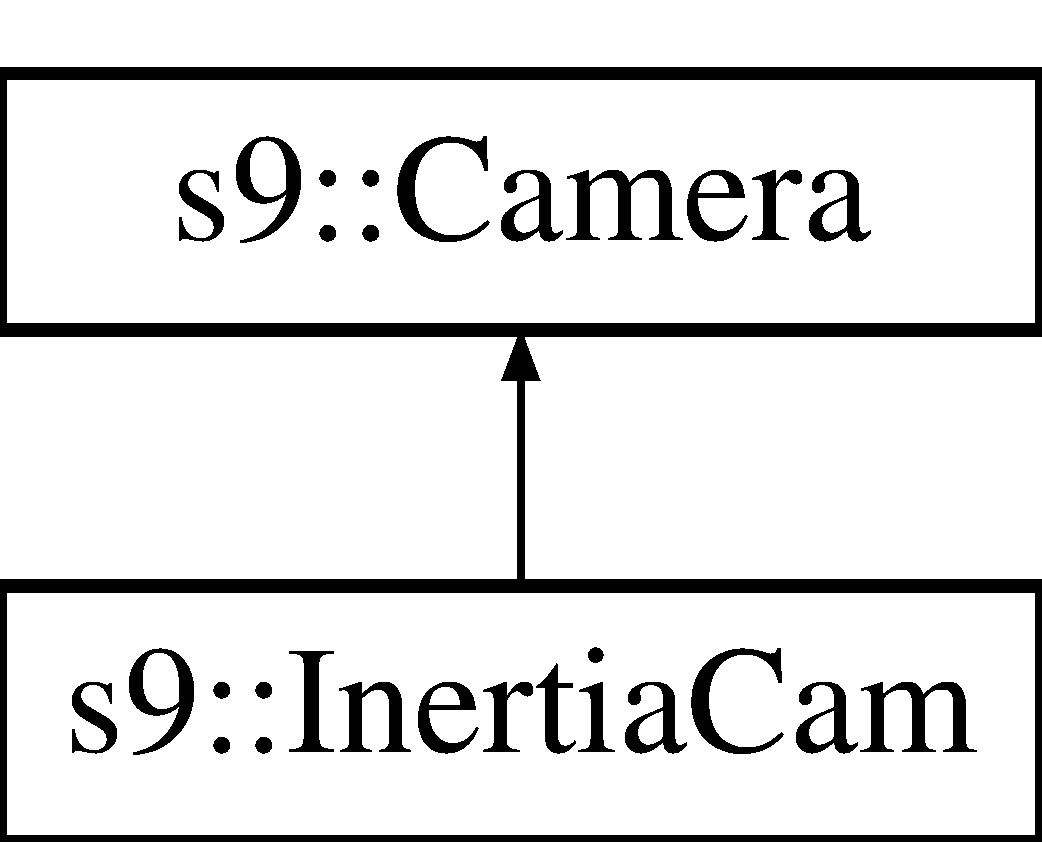
\includegraphics[height=2.000000cm]{classs9_1_1Camera}
\end{center}
\end{figure}
\subsection*{\-Public \-Member \-Functions}
\begin{DoxyCompactItemize}
\item 
\hypertarget{classs9_1_1Camera_a6eff9242a0e38236d26c0b5b8934c23e}{void {\bfseries resize} (size\-\_\-t w, size\-\_\-t h)}\label{classs9_1_1Camera_a6eff9242a0e38236d26c0b5b8934c23e}

\item 
\hypertarget{classs9_1_1Camera_a187249f6840355e90385d77c07139541}{void {\bfseries set\-\_\-near} (float n)}\label{classs9_1_1Camera_a187249f6840355e90385d77c07139541}

\item 
\hypertarget{classs9_1_1Camera_a495b9d2c12ab823c3f0d5fc60ccd9037}{void {\bfseries set\-\_\-far} (float n)}\label{classs9_1_1Camera_a495b9d2c12ab823c3f0d5fc60ccd9037}

\item 
\hypertarget{classs9_1_1Camera_a1bb91a852163fe9ddf31468abcf0813e}{void {\bfseries set\-\_\-ratio} (float r)}\label{classs9_1_1Camera_a1bb91a852163fe9ddf31468abcf0813e}

\item 
\hypertarget{classs9_1_1Camera_a738b170a72c097cc5c834335f06dd641}{void {\bfseries set\-\_\-field} (float a)}\label{classs9_1_1Camera_a738b170a72c097cc5c834335f06dd641}

\item 
\hypertarget{classs9_1_1Camera_a03479cc99295b235cbab0c019e68660d}{glm\-::vec3 {\bfseries pos} ()}\label{classs9_1_1Camera_a03479cc99295b235cbab0c019e68660d}

\item 
\hypertarget{classs9_1_1Camera_a8a0711b866e4278587c0d2e65c0f510e}{glm\-::vec3 {\bfseries look} ()}\label{classs9_1_1Camera_a8a0711b866e4278587c0d2e65c0f510e}

\item 
\hypertarget{classs9_1_1Camera_a1e2bd41a35c04d3b067f81838fe97020}{glm\-::vec3 {\bfseries up} ()}\label{classs9_1_1Camera_a1e2bd41a35c04d3b067f81838fe97020}

\item 
\hypertarget{classs9_1_1Camera_ae3fe7ead9bd092788f2a6e03059d0c44}{void {\bfseries zoom} (float z)}\label{classs9_1_1Camera_ae3fe7ead9bd092788f2a6e03059d0c44}

\item 
\hypertarget{classs9_1_1Camera_a91f4d7b8eeead328fc7f7032ca65028d}{void {\bfseries shift} (glm\-::vec2 s)}\label{classs9_1_1Camera_a91f4d7b8eeead328fc7f7032ca65028d}

\item 
\hypertarget{classs9_1_1Camera_a91306d514cfb18f27a5738db7fa333fe}{void {\bfseries yaw} (float a)}\label{classs9_1_1Camera_a91306d514cfb18f27a5738db7fa333fe}

\item 
\hypertarget{classs9_1_1Camera_abdb854cd3faba278f3f8ce3557fb659a}{void {\bfseries pitch} (float a)}\label{classs9_1_1Camera_abdb854cd3faba278f3f8ce3557fb659a}

\item 
\hypertarget{classs9_1_1Camera_aed1349816f0b99f6afe44aeea0d176a2}{void {\bfseries roll} (float a)}\label{classs9_1_1Camera_aed1349816f0b99f6afe44aeea0d176a2}

\item 
\hypertarget{classs9_1_1Camera_adfd093ba7497106216056072c3204218}{void {\bfseries set\-\_\-orthographic} (bool b)}\label{classs9_1_1Camera_adfd093ba7497106216056072c3204218}

\item 
\hypertarget{classs9_1_1Camera_aee4419400067cfcfc26f9864328d7cbd}{bool {\bfseries orthographic} ()}\label{classs9_1_1Camera_aee4419400067cfcfc26f9864328d7cbd}

\item 
\hypertarget{classs9_1_1Camera_a02be8aa0dbef77e02dddc715a726fb67}{void {\bfseries reset} ()}\label{classs9_1_1Camera_a02be8aa0dbef77e02dddc715a726fb67}

\item 
\hypertarget{classs9_1_1Camera_a06254a1642d663e024e1b34c8e5f59ca}{void {\bfseries set\-\_\-pos} (glm\-::vec3 p)}\label{classs9_1_1Camera_a06254a1642d663e024e1b34c8e5f59ca}

\item 
\hypertarget{classs9_1_1Camera_afc53e7e53b952e36dc55a355dfb81958}{void {\bfseries set\-\_\-look} (glm\-::vec3 p)}\label{classs9_1_1Camera_afc53e7e53b952e36dc55a355dfb81958}

\item 
\hypertarget{classs9_1_1Camera_a02b59733a720549bdc955d48a1b3ff97}{void {\bfseries set\-\_\-up} (glm\-::vec3 p)}\label{classs9_1_1Camera_a02b59733a720549bdc955d48a1b3ff97}

\item 
\hypertarget{classs9_1_1Camera_a059cec22aa650e270b95b322bc5aa9a7}{void {\bfseries set\-\_\-left} (size\-\_\-t p)}\label{classs9_1_1Camera_a059cec22aa650e270b95b322bc5aa9a7}

\item 
\hypertarget{classs9_1_1Camera_a0d40f3e9b239cf6979a34b1df0a9764d}{void {\bfseries set\-\_\-top} (size\-\_\-t p)}\label{classs9_1_1Camera_a0d40f3e9b239cf6979a34b1df0a9764d}

\item 
\hypertarget{classs9_1_1Camera_a2c164ccc92ccca8ea2bb81d8eb779023}{void {\bfseries set\-\_\-right} (size\-\_\-t p)}\label{classs9_1_1Camera_a2c164ccc92ccca8ea2bb81d8eb779023}

\item 
\hypertarget{classs9_1_1Camera_ad1e6a888b424e32632ff4a795e0f2c8d}{void {\bfseries set\-\_\-bottom} (size\-\_\-t p)}\label{classs9_1_1Camera_ad1e6a888b424e32632ff4a795e0f2c8d}

\item 
\hypertarget{classs9_1_1Camera_a7e9cc98105e567636c4eebca453b5d9d}{glm\-::mat4 {\bfseries view\-\_\-matrix} ()}\label{classs9_1_1Camera_a7e9cc98105e567636c4eebca453b5d9d}

\item 
\hypertarget{classs9_1_1Camera_a9ee97b1396546c43115190de8405cf27}{glm\-::mat4 {\bfseries projection\-\_\-matrix} ()}\label{classs9_1_1Camera_a9ee97b1396546c43115190de8405cf27}

\item 
\hypertarget{classs9_1_1Camera_a42cda7239981a5618660d04bd5893556}{virtual void {\bfseries update} ()}\label{classs9_1_1Camera_a42cda7239981a5618660d04bd5893556}

\item 
\hypertarget{classs9_1_1Camera_a4367ec82119e3fe249d744d420875f3d}{virtual void {\bfseries update} (double\-\_\-t dt)}\label{classs9_1_1Camera_a4367ec82119e3fe249d744d420875f3d}

\end{DoxyCompactItemize}
\subsection*{\-Protected \-Attributes}
\begin{DoxyCompactItemize}
\item 
\hypertarget{classs9_1_1Camera_aa14bf0dbfe9f292b4841c647f328dd76}{glm\-::mat4 {\bfseries view\-\_\-matrix\-\_\-}}\label{classs9_1_1Camera_aa14bf0dbfe9f292b4841c647f328dd76}

\item 
\hypertarget{classs9_1_1Camera_aab7a588b390fa05250f25b5538e46b86}{glm\-::mat4 {\bfseries projection\-\_\-matrix\-\_\-}}\label{classs9_1_1Camera_aab7a588b390fa05250f25b5538e46b86}

\item 
\hypertarget{classs9_1_1Camera_a71665686599a0151fad513544fa21230}{bool {\bfseries orthographic\-\_\-}}\label{classs9_1_1Camera_a71665686599a0151fad513544fa21230}

\item 
\hypertarget{classs9_1_1Camera_a0344aaaadb55b0d81800b51f2c7b2815}{float {\bfseries ratio\-\_\-}}\label{classs9_1_1Camera_a0344aaaadb55b0d81800b51f2c7b2815}

\item 
\hypertarget{classs9_1_1Camera_a3756d83d24d11222efa0130e95ff903e}{float {\bfseries far\-\_\-}}\label{classs9_1_1Camera_a3756d83d24d11222efa0130e95ff903e}

\item 
\hypertarget{classs9_1_1Camera_a214dd980fd5f99f272e1aef1646e45e4}{float {\bfseries near\-\_\-}}\label{classs9_1_1Camera_a214dd980fd5f99f272e1aef1646e45e4}

\item 
\hypertarget{classs9_1_1Camera_a88cb54b968bf47fea6a536fba0ab52e8}{float {\bfseries field\-\_\-}}\label{classs9_1_1Camera_a88cb54b968bf47fea6a536fba0ab52e8}

\item 
\hypertarget{classs9_1_1Camera_aae3f13ab7467694c6b38175e1df84a76}{size\-\_\-t {\bfseries left\-\_\-}}\label{classs9_1_1Camera_aae3f13ab7467694c6b38175e1df84a76}

\item 
\hypertarget{classs9_1_1Camera_aff5887222b004435324ef1d37a2b20d6}{size\-\_\-t {\bfseries top\-\_\-}}\label{classs9_1_1Camera_aff5887222b004435324ef1d37a2b20d6}

\item 
\hypertarget{classs9_1_1Camera_a39f17ec5ca1d58c0e91c544f6aa4e38b}{size\-\_\-t {\bfseries bottom\-\_\-}}\label{classs9_1_1Camera_a39f17ec5ca1d58c0e91c544f6aa4e38b}

\item 
\hypertarget{classs9_1_1Camera_ad56ce0d5e3a1bc7ccd0e993ef93ae171}{size\-\_\-t {\bfseries right\-\_\-}}\label{classs9_1_1Camera_ad56ce0d5e3a1bc7ccd0e993ef93ae171}

\item 
\hypertarget{classs9_1_1Camera_ad0e9f3951aea84ed9dcf22391d123f35}{glm\-::vec3 {\bfseries pos\-\_\-}}\label{classs9_1_1Camera_ad0e9f3951aea84ed9dcf22391d123f35}

\item 
\hypertarget{classs9_1_1Camera_ab7be66338e1ed45f7e7721089c7644ef}{glm\-::vec3 {\bfseries look\-\_\-}}\label{classs9_1_1Camera_ab7be66338e1ed45f7e7721089c7644ef}

\item 
\hypertarget{classs9_1_1Camera_a193b633a02c7c6dd1055d97d8f09baa4}{glm\-::vec3 {\bfseries up\-\_\-}}\label{classs9_1_1Camera_a193b633a02c7c6dd1055d97d8f09baa4}

\end{DoxyCompactItemize}


\-The documentation for this class was generated from the following files\-:\begin{DoxyCompactItemize}
\item 
include/s9/\hyperlink{camera_8hpp}{camera.\-hpp}\item 
src/\hyperlink{camera_8cpp}{camera.\-cpp}\end{DoxyCompactItemize}

\hypertarget{structcomp}{\section{comp Struct Reference}
\label{structcomp}\index{comp@{comp}}
}
\subsection*{Public Attributes}
\begin{DoxyCompactItemize}
\item 
\hypertarget{structcomp_a8a13b7d6171a6411afc68ab9c6cd792d}{int {\bfseries cid}}\label{structcomp_a8a13b7d6171a6411afc68ab9c6cd792d}

\item 
\hypertarget{structcomp_ae9b94231445da3c4fce322ae12cd82a8}{int {\bfseries hv}}\label{structcomp_ae9b94231445da3c4fce322ae12cd82a8}

\item 
\hypertarget{structcomp_a4fb10c419453e686d29787651ba299dc}{int {\bfseries tq}}\label{structcomp_a4fb10c419453e686d29787651ba299dc}

\end{DoxyCompactItemize}


The documentation for this struct was generated from the following file\-:\begin{DoxyCompactItemize}
\item 
src/linux/jpeg.\-c\end{DoxyCompactItemize}

\hypertarget{structs9_1_1CompileTimeChecker}{\section{s9\-:\-:Compile\-Time\-Checker$<$ bool $>$ Struct Template Reference}
\label{structs9_1_1CompileTimeChecker}\index{s9\-::\-Compile\-Time\-Checker$<$ bool $>$@{s9\-::\-Compile\-Time\-Checker$<$ bool $>$}}
}


{\ttfamily \#include $<$utils.\-hpp$>$}

\subsection*{Public Member Functions}
\begin{DoxyCompactItemize}
\item 
\hypertarget{structs9_1_1CompileTimeChecker_a53515adf153a125605e1df2e41f31e6d}{{\bfseries Compile\-Time\-Checker} (...)}\label{structs9_1_1CompileTimeChecker_a53515adf153a125605e1df2e41f31e6d}

\end{DoxyCompactItemize}


\subsection{Detailed Description}
\subsubsection*{template$<$bool$>$struct s9\-::\-Compile\-Time\-Checker$<$ bool $>$}

Checking at Compile Time Modern C++ Design\-: Applied Generic and Design Patterns (C++ in Depth) 

The documentation for this struct was generated from the following file\-:\begin{DoxyCompactItemize}
\item 
include/s9/utils.\-hpp\end{DoxyCompactItemize}

\hypertarget{structs9_1_1CompileTimeChecker_3_01false_01_4}{\section{s9\-:\-:\-Compile\-Time\-Checker$<$ false $>$ \-Struct \-Template \-Reference}
\label{structs9_1_1CompileTimeChecker_3_01false_01_4}\index{s9\-::\-Compile\-Time\-Checker$<$ false $>$@{s9\-::\-Compile\-Time\-Checker$<$ false $>$}}
}
\subsubsection*{template$<$$>$ struct s9\-::\-Compile\-Time\-Checker$<$ false $>$}



\-The documentation for this struct was generated from the following file\-:\begin{DoxyCompactItemize}
\item 
include/s9/utils.\-hpp\end{DoxyCompactItemize}

\hypertarget{classs9_1_1Cuboid}{\section{s9\-:\-:Cuboid Class Reference}
\label{classs9_1_1Cuboid}\index{s9\-::\-Cuboid@{s9\-::\-Cuboid}}
}
Inheritance diagram for s9\-:\-:Cuboid\-:\begin{figure}[H]
\begin{center}
\leavevmode
\includegraphics[height=2.000000cm]{classs9_1_1Cuboid}
\end{center}
\end{figure}
\subsection*{Public Member Functions}
\begin{DoxyCompactItemize}
\item 
\hyperlink{classs9_1_1Cuboid_a26c36d171baec9aaa7dfac6a78d125b7}{Cuboid} (float w, float h, float d)
\item 
\hypertarget{classs9_1_1Cuboid_a407f0775eb66c4d3932f9b1c256386f5}{const \hyperlink{classs9_1_1GeometryT}{Geometry\-T}$<$ \hyperlink{structs9_1_1VertexT}{Vertex4}, \\*
\hyperlink{structs9_1_1FaceT}{Face4}, \hyperlink{classs9_1_1AllocationPolicyNew}{Allocation\-Policy\-New} $>$ $\ast$ {\bfseries geometry} ()}\label{classs9_1_1Cuboid_a407f0775eb66c4d3932f9b1c256386f5}

\end{DoxyCompactItemize}
\subsection*{Additional Inherited Members}


\subsection{Constructor \& Destructor Documentation}
\hypertarget{classs9_1_1Cuboid_a26c36d171baec9aaa7dfac6a78d125b7}{\index{s9\-::\-Cuboid@{s9\-::\-Cuboid}!Cuboid@{Cuboid}}
\index{Cuboid@{Cuboid}!s9::Cuboid@{s9\-::\-Cuboid}}
\subsubsection[{Cuboid}]{\setlength{\rightskip}{0pt plus 5cm}Cuboid\-::\-Cuboid (
\begin{DoxyParamCaption}
\item[{float}]{w, }
\item[{float}]{h, }
\item[{float}]{d}
\end{DoxyParamCaption}
)}}\label{classs9_1_1Cuboid_a26c36d171baec9aaa7dfac6a78d125b7}
Build a \hyperlink{classs9_1_1Cuboid}{Cuboid} with w,h,d centred at the origin 

The documentation for this class was generated from the following files\-:\begin{DoxyCompactItemize}
\item 
include/s9/\hyperlink{shapes_8hpp}{shapes.\-hpp}\item 
src/\hyperlink{shapes_8cpp}{shapes.\-cpp}\end{DoxyCompactItemize}

\hypertarget{structdec__hufftbl}{\section{dec\-\_\-hufftbl Struct Reference}
\label{structdec__hufftbl}\index{dec\-\_\-hufftbl@{dec\-\_\-hufftbl}}
}
\subsection*{Public Attributes}
\begin{DoxyCompactItemize}
\item 
\hypertarget{structdec__hufftbl_a8b500876289dda1731ca4360ed8dc4e6}{int {\bfseries maxcode} \mbox{[}17\mbox{]}}\label{structdec__hufftbl_a8b500876289dda1731ca4360ed8dc4e6}

\item 
\hypertarget{structdec__hufftbl_a4011f65e72d693639c5a353c386a7519}{int {\bfseries valptr} \mbox{[}16\mbox{]}}\label{structdec__hufftbl_a4011f65e72d693639c5a353c386a7519}

\item 
\hypertarget{structdec__hufftbl_a91e35217d39149d2f98b896f65d0bc33}{B\-Y\-T\-E {\bfseries vals} \mbox{[}256\mbox{]}}\label{structdec__hufftbl_a91e35217d39149d2f98b896f65d0bc33}

\item 
\hypertarget{structdec__hufftbl_a286111323bdb40b2032f7c441f9c311d}{D\-W\-O\-R\-D {\bfseries llvals} \mbox{[}1$<$$<$ D\-E\-C\-B\-I\-T\-S\mbox{]}}\label{structdec__hufftbl_a286111323bdb40b2032f7c441f9c311d}

\end{DoxyCompactItemize}


The documentation for this struct was generated from the following file\-:\begin{DoxyCompactItemize}
\item 
include/s9/jpeg.\-h\end{DoxyCompactItemize}

\hypertarget{structs9_1_1oculus_1_1OculusBase_1_1DeviceStatusNotificationDesc}{\section{s9\-:\-:oculus\-:\-:Oculus\-Base\-:\-:Device\-Status\-Notification\-Desc Struct Reference}
\label{structs9_1_1oculus_1_1OculusBase_1_1DeviceStatusNotificationDesc}\index{s9\-::oculus\-::\-Oculus\-Base\-::\-Device\-Status\-Notification\-Desc@{s9\-::oculus\-::\-Oculus\-Base\-::\-Device\-Status\-Notification\-Desc}}
}
\subsection*{Public Member Functions}
\begin{DoxyCompactItemize}
\item 
\hypertarget{structs9_1_1oculus_1_1OculusBase_1_1DeviceStatusNotificationDesc_ab9ba774f4572708770ad28dfafeb84dc}{{\bfseries Device\-Status\-Notification\-Desc} (O\-V\-R\-::\-Message\-Type mt, const O\-V\-R\-::\-Device\-Handle \&dev)}\label{structs9_1_1oculus_1_1OculusBase_1_1DeviceStatusNotificationDesc_ab9ba774f4572708770ad28dfafeb84dc}

\end{DoxyCompactItemize}
\subsection*{Public Attributes}
\begin{DoxyCompactItemize}
\item 
\hypertarget{structs9_1_1oculus_1_1OculusBase_1_1DeviceStatusNotificationDesc_a64c6d955e46160eb5e0b31e5cd769b22}{O\-V\-R\-::\-Device\-Handle {\bfseries Handle}}\label{structs9_1_1oculus_1_1OculusBase_1_1DeviceStatusNotificationDesc_a64c6d955e46160eb5e0b31e5cd769b22}

\item 
\hypertarget{structs9_1_1oculus_1_1OculusBase_1_1DeviceStatusNotificationDesc_a2a4e88e7c6ff451ee9cb6f6212509923}{O\-V\-R\-::\-Message\-Type {\bfseries Action}}\label{structs9_1_1oculus_1_1OculusBase_1_1DeviceStatusNotificationDesc_a2a4e88e7c6ff451ee9cb6f6212509923}

\end{DoxyCompactItemize}


The documentation for this struct was generated from the following file\-:\begin{DoxyCompactItemize}
\item 
include/s9/oculus/\hyperlink{oculus_8hpp}{oculus.\-hpp}\end{DoxyCompactItemize}

\hypertarget{classs9_1_1gl_1_1Drawable}{\section{s9\-:\-:gl\-:\-:\-Drawable \-Class \-Reference}
\label{classs9_1_1gl_1_1Drawable}\index{s9\-::gl\-::\-Drawable@{s9\-::gl\-::\-Drawable}}
}


{\ttfamily \#include $<$drawable.\-hpp$>$}

\subsection*{\-Public \-Member \-Functions}
\begin{DoxyCompactItemize}
\item 
{\footnotesize template$<$typename Vertex\-Type , typename Face\-Type , typename Allocation\-Policy $>$ }\\void \hyperlink{classs9_1_1gl_1_1Drawable_a17009f367a17d45ac7f9245b15229c95}{draw} (\hyperlink{classs9_1_1GeometryT}{\-Geometry\-T}$<$ \-Vertex\-Type, \-Face\-Type, \-Allocation\-Policy $>$ \&g, \hyperlink{namespaces9_ad57d1332f8fd67d23f6a1d3520ab785c}{\-Geometry\-Primitive} gp)
\item 
{\footnotesize template$<$typename Vertex\-Type , typename Face\-Type , typename Allocation\-Policy $>$ }\\void \hyperlink{classs9_1_1gl_1_1Drawable_ac45a196466c96705860cff9f8898673f}{brew} (\hyperlink{classs9_1_1GeometryT}{\-Geometry\-T}$<$ \-Vertex\-Type, \-Face\-Type, \-Allocation\-Policy $>$ \&g, \hyperlink{structs9_1_1gl_1_1BrewFlags}{\-Brew\-Flags} b=\-Brew\-Flags\-Default)
\item 
\hypertarget{classs9_1_1gl_1_1Drawable_ae616cb10c8f213e08914acb760e0a087}{void {\bfseries bind} ()}\label{classs9_1_1gl_1_1Drawable_ae616cb10c8f213e08914acb760e0a087}

\item 
\hypertarget{classs9_1_1gl_1_1Drawable_a6a55c040167e67f808adce694ae425f5}{void {\bfseries unbind} ()}\label{classs9_1_1gl_1_1Drawable_a6a55c040167e67f808adce694ae425f5}

\end{DoxyCompactItemize}
\subsection*{\-Protected \-Member \-Functions}
\begin{DoxyCompactItemize}
\item 
{\footnotesize template$<$typename Vertex\-Type , typename Face\-Type , typename Allocation\-Policy $>$ }\\void \hyperlink{classs9_1_1gl_1_1Drawable_ad9c83ff9377dfd128a32e2bb005d257f}{allocate} (\hyperlink{classs9_1_1GeometryT}{\-Geometry\-T}$<$ \-Vertex\-Type, \-Face\-Type, \-Allocation\-Policy $>$ \&g, \hyperlink{structs9_1_1gl_1_1BrewFlags}{\-Brew\-Flags} b)
\item 
\hypertarget{classs9_1_1gl_1_1Drawable_a262ce388ff43ede822f61c96272c7747}{{\footnotesize template$<$typename Allocation\-Policy $>$ }\\void {\bfseries allocate} (\hyperlink{classs9_1_1GeometryT}{\-Geometry\-T}$<$ \hyperlink{structs9_1_1VertexT}{\-Vertex2}, \hyperlink{structs9_1_1FaceT}{\-Face3}, \-Allocation\-Policy $>$ \&g, \hyperlink{structs9_1_1gl_1_1BrewFlags}{\-Brew\-Flags} b)}\label{classs9_1_1gl_1_1Drawable_a262ce388ff43ede822f61c96272c7747}

\item 
\hypertarget{classs9_1_1gl_1_1Drawable_a4489c6f70638b5d75558349225cd43a8}{{\footnotesize template$<$typename Allocation\-Policy $>$ }\\void {\bfseries allocate} (\hyperlink{classs9_1_1GeometryT}{\-Geometry\-T}$<$ \hyperlink{structs9_1_1VertexT}{\-Vertex3}, \hyperlink{structs9_1_1FaceT}{\-Face3}, \-Allocation\-Policy $>$ \&g, \hyperlink{structs9_1_1gl_1_1BrewFlags}{\-Brew\-Flags} b)}\label{classs9_1_1gl_1_1Drawable_a4489c6f70638b5d75558349225cd43a8}

\item 
\hypertarget{classs9_1_1gl_1_1Drawable_a17ad8176a4295ec65e12ef4bb316581a}{{\footnotesize template$<$typename Allocation\-Policy $>$ }\\void {\bfseries allocate} (\hyperlink{classs9_1_1GeometryT}{\-Geometry\-T}$<$ \hyperlink{structs9_1_1VertexT}{\-Vertex4}, \hyperlink{structs9_1_1FaceT}{\-Face3}, \-Allocation\-Policy $>$ \&g, \hyperlink{structs9_1_1gl_1_1BrewFlags}{\-Brew\-Flags} b)}\label{classs9_1_1gl_1_1Drawable_a17ad8176a4295ec65e12ef4bb316581a}

\item 
\hypertarget{classs9_1_1gl_1_1Drawable_ac984e096084672fd0ffcef1560ab8b11}{{\footnotesize template$<$typename Allocation\-Policy $>$ }\\void {\bfseries allocate} (\hyperlink{classs9_1_1GeometryT}{\-Geometry\-T}$<$ \hyperlink{structs9_1_1VertexT}{\-Vertex2}, \hyperlink{structs9_1_1FaceT}{\-Face4}, \-Allocation\-Policy $>$ \&g, \hyperlink{structs9_1_1gl_1_1BrewFlags}{\-Brew\-Flags} b)}\label{classs9_1_1gl_1_1Drawable_ac984e096084672fd0ffcef1560ab8b11}

\item 
\hypertarget{classs9_1_1gl_1_1Drawable_a9df92ec26ccfddc5a49b9f440e62c69f}{{\footnotesize template$<$typename Allocation\-Policy $>$ }\\void {\bfseries allocate} (\hyperlink{classs9_1_1GeometryT}{\-Geometry\-T}$<$ \hyperlink{structs9_1_1VertexT}{\-Vertex3}, \hyperlink{structs9_1_1FaceT}{\-Face4}, \-Allocation\-Policy $>$ \&g, \hyperlink{structs9_1_1gl_1_1BrewFlags}{\-Brew\-Flags} b)}\label{classs9_1_1gl_1_1Drawable_a9df92ec26ccfddc5a49b9f440e62c69f}

\item 
\hypertarget{classs9_1_1gl_1_1Drawable_a6033b5801d330cd6fa2994fc8a77fab6}{{\footnotesize template$<$typename Allocation\-Policy $>$ }\\void {\bfseries allocate} (\hyperlink{classs9_1_1GeometryT}{\-Geometry\-T}$<$ \hyperlink{structs9_1_1VertexT}{\-Vertex4}, \hyperlink{structs9_1_1FaceT}{\-Face4}, \-Allocation\-Policy $>$ \&g, \hyperlink{structs9_1_1gl_1_1BrewFlags}{\-Brew\-Flags} b)}\label{classs9_1_1gl_1_1Drawable_a6033b5801d330cd6fa2994fc8a77fab6}

\item 
\hypertarget{classs9_1_1gl_1_1Drawable_a9cf81e2a6d53700488217b215a5d741f}{{\footnotesize template$<$typename Vertex\-Type , typename Face\-Type , typename Allocation\-Policy $>$ }\\void {\bfseries set\-Pointers} (\hyperlink{classs9_1_1GeometryT}{\-Geometry\-T}$<$ \-Vertex\-Type, \-Face\-Type, \-Allocation\-Policy $>$ \&g, \hyperlink{structs9_1_1gl_1_1BrewFlags}{\-Brew\-Flags} b)}\label{classs9_1_1gl_1_1Drawable_a9cf81e2a6d53700488217b215a5d741f}

\item 
{\footnotesize template$<$typename Allocation\-Policy $>$ }\\void \hyperlink{classs9_1_1gl_1_1Drawable_a82268b69a4127ccea73e20d14e9a4835}{set\-Pointers} (\hyperlink{classs9_1_1GeometryT}{\-Geometry\-T}$<$ \hyperlink{structs9_1_1VertexT}{\-Vertex4}, \hyperlink{structs9_1_1FaceT}{\-Face4}, \-Allocation\-Policy $>$ \&g, \hyperlink{structs9_1_1gl_1_1BrewFlags}{\-Brew\-Flags} b)
\end{DoxyCompactItemize}
\subsection*{\-Protected \-Attributes}
\begin{DoxyCompactItemize}
\item 
\hypertarget{classs9_1_1gl_1_1Drawable_af6cf679ad222fb978916db2d2123b6ad}{\-G\-Luint {\bfseries vao\-\_\-}}\label{classs9_1_1gl_1_1Drawable_af6cf679ad222fb978916db2d2123b6ad}

\item 
\hypertarget{classs9_1_1gl_1_1Drawable_a8fb7244c60f78807837526c482e8965b}{std\-::vector$<$ unsigned int $>$ {\bfseries handles\-\_\-}}\label{classs9_1_1gl_1_1Drawable_a8fb7244c60f78807837526c482e8965b}

\end{DoxyCompactItemize}


\subsection{\-Detailed \-Description}
\hyperlink{classs9_1_1gl_1_1Drawable}{\-Drawable} \-Class -\/ \-Provides functionality to the \hyperlink{classs9_1_1Shape}{\-Shape} class, allowing it to be drawn to the screen. \-Keeps track of buffers but only holds primitive types \-This is loosely coupled with its geometry, only at brew time. 

\subsection{\-Member \-Function \-Documentation}
\hypertarget{classs9_1_1gl_1_1Drawable_ad9c83ff9377dfd128a32e2bb005d257f}{\index{s9\-::gl\-::\-Drawable@{s9\-::gl\-::\-Drawable}!allocate@{allocate}}
\index{allocate@{allocate}!s9::gl::Drawable@{s9\-::gl\-::\-Drawable}}
\subsubsection[{allocate}]{\setlength{\rightskip}{0pt plus 5cm}template$<$typename Vertex\-Type , typename Face\-Type , typename Allocation\-Policy $>$ void {\bf s9\-::gl\-::\-Drawable\-::allocate} (
\begin{DoxyParamCaption}
\item[{{\bf \-Geometry\-T}$<$ \-Vertex\-Type, \-Face\-Type, \-Allocation\-Policy $>$ \&}]{g, }
\item[{{\bf \-Brew\-Flags}}]{b}
\end{DoxyParamCaption}
)\hspace{0.3cm}{\ttfamily  \mbox{[}inline, protected\mbox{]}}}}\label{classs9_1_1gl_1_1Drawable_ad9c83ff9377dfd128a32e2bb005d257f}
allocation of the data into the buffer -\/ copy to the card default template function should never be called. \hypertarget{classs9_1_1gl_1_1Drawable_ac45a196466c96705860cff9f8898673f}{\index{s9\-::gl\-::\-Drawable@{s9\-::gl\-::\-Drawable}!brew@{brew}}
\index{brew@{brew}!s9::gl::Drawable@{s9\-::gl\-::\-Drawable}}
\subsubsection[{brew}]{\setlength{\rightskip}{0pt plus 5cm}template$<$typename Vertex\-Type , typename Face\-Type , typename Allocation\-Policy $>$ void {\bf s9\-::gl\-::\-Drawable\-::brew} (
\begin{DoxyParamCaption}
\item[{{\bf \-Geometry\-T}$<$ \-Vertex\-Type, \-Face\-Type, \-Allocation\-Policy $>$ \&}]{g, }
\item[{{\bf \-Brew\-Flags}}]{b = {\ttfamily \-Brew\-Flags\-Default}}
\end{DoxyParamCaption}
)\hspace{0.3cm}{\ttfamily  \mbox{[}inline\mbox{]}}}}\label{classs9_1_1gl_1_1Drawable_ac45a196466c96705860cff9f8898673f}
\begin{DoxyRefDesc}{\-Todo}
\item[\hyperlink{todo__todo000018}{\-Todo}]non interleaved buffers \end{DoxyRefDesc}


\-Last handle is always the indices \hypertarget{classs9_1_1gl_1_1Drawable_a17009f367a17d45ac7f9245b15229c95}{\index{s9\-::gl\-::\-Drawable@{s9\-::gl\-::\-Drawable}!draw@{draw}}
\index{draw@{draw}!s9::gl::Drawable@{s9\-::gl\-::\-Drawable}}
\subsubsection[{draw}]{\setlength{\rightskip}{0pt plus 5cm}template$<$typename Vertex\-Type , typename Face\-Type , typename Allocation\-Policy $>$ void {\bf s9\-::gl\-::\-Drawable\-::draw} (
\begin{DoxyParamCaption}
\item[{{\bf \-Geometry\-T}$<$ \-Vertex\-Type, \-Face\-Type, \-Allocation\-Policy $>$ \&}]{g, }
\item[{{\bf \-Geometry\-Primitive}}]{gp}
\end{DoxyParamCaption}
)\hspace{0.3cm}{\ttfamily  \mbox{[}inline\mbox{]}}}}\label{classs9_1_1gl_1_1Drawable_a17009f367a17d45ac7f9245b15229c95}
\begin{DoxyRefDesc}{\-Todo}
\item[\hyperlink{todo__todo000016}{\-Todo}]unbrew method for cleaning data off the card \-Options for brewing that may need to be specified \end{DoxyRefDesc}
\begin{DoxyRefDesc}{\-Todo}
\item[\hyperlink{todo__todo000017}{\-Todo}]indices type matching \-G\-L\-\_\-\-U\-N\-S\-I\-G\-N\-E\-D\-\_\-\-I\-N\-T \end{DoxyRefDesc}
\hypertarget{classs9_1_1gl_1_1Drawable_a82268b69a4127ccea73e20d14e9a4835}{\index{s9\-::gl\-::\-Drawable@{s9\-::gl\-::\-Drawable}!set\-Pointers@{set\-Pointers}}
\index{set\-Pointers@{set\-Pointers}!s9::gl::Drawable@{s9\-::gl\-::\-Drawable}}
\subsubsection[{set\-Pointers}]{\setlength{\rightskip}{0pt plus 5cm}template$<$typename Allocation\-Policy $>$ void s9\-::gl\-::\-Drawable\-::set\-Pointers (
\begin{DoxyParamCaption}
\item[{{\bf \-Geometry\-T}$<$ {\bf \-Vertex4}, {\bf \-Face4}, \-Allocation\-Policy $>$ \&}]{g, }
\item[{{\bf \-Brew\-Flags}}]{b}
\end{DoxyParamCaption}
)\hspace{0.3cm}{\ttfamily  \mbox{[}inline, protected\mbox{]}}}}\label{classs9_1_1gl_1_1Drawable_a82268b69a4127ccea73e20d14e9a4835}
\begin{DoxyRefDesc}{\-Todo}
\item[\hyperlink{todo__todo000019}{\-Todo}]\-G\-L\-\_\-\-U\-N\-S\-I\-G\-N\-E\-D\-\_\-\-I\-N\-T must match the \-Indicies\-Type \end{DoxyRefDesc}


\-The documentation for this class was generated from the following file\-:\begin{DoxyCompactItemize}
\item 
include/s9/gl/\hyperlink{drawable_8hpp}{drawable.\-hpp}\end{DoxyCompactItemize}

\hypertarget{structs9_1_1Event}{\section{s9\-:\-:Event Struct Reference}
\label{structs9_1_1Event}\index{s9\-::\-Event@{s9\-::\-Event}}
}
Inheritance diagram for s9\-:\-:Event\-:\begin{figure}[H]
\begin{center}
\leavevmode
\includegraphics[height=2.000000cm]{structs9_1_1Event}
\end{center}
\end{figure}
\subsection*{Public Attributes}
\begin{DoxyCompactItemize}
\item 
\hypertarget{structs9_1_1Event_ac6d2a02aeab6cd0c5ffd05d67fcb71f0}{Event\-Type {\bfseries type}}\label{structs9_1_1Event_ac6d2a02aeab6cd0c5ffd05d67fcb71f0}

\item 
\hypertarget{structs9_1_1Event_a600210822b48f7a2f88c9acb3f0d2088}{double\-\_\-t {\bfseries t}}\label{structs9_1_1Event_a600210822b48f7a2f88c9acb3f0d2088}

\end{DoxyCompactItemize}
\subsection*{Friends}
\begin{DoxyCompactItemize}
\item 
\hypertarget{structs9_1_1Event_a7789ff8e8663c0ff98d2758bbf41116e}{std\-::ostream \& {\bfseries operator$<$$<$} (std\-::ostream \&out, const \hyperlink{structs9_1_1Event}{Event} \&o)}\label{structs9_1_1Event_a7789ff8e8663c0ff98d2758bbf41116e}

\end{DoxyCompactItemize}


The documentation for this struct was generated from the following file\-:\begin{DoxyCompactItemize}
\item 
include/s9/events.\-hpp\end{DoxyCompactItemize}

\hypertarget{structs9_1_1FaceT}{\section{s9\-:\-:Face\-T$<$ T $>$ Struct Template Reference}
\label{structs9_1_1FaceT}\index{s9\-::\-Face\-T$<$ T $>$@{s9\-::\-Face\-T$<$ T $>$}}
}


{\ttfamily \#include $<$primitives.\-hpp$>$}

\subsection*{Public Member Functions}
\begin{DoxyCompactItemize}
\item 
\hypertarget{structs9_1_1FaceT_aea08fe5c720cb7583848e6b607e08578}{{\bfseries Face\-T} (const T pn=T(1.\-0f), const T pc=\-T(1.\-0f))}\label{structs9_1_1FaceT_aea08fe5c720cb7583848e6b607e08578}

\end{DoxyCompactItemize}
\subsection*{Public Attributes}
\begin{DoxyCompactItemize}
\item 
\hypertarget{structs9_1_1FaceT_a7d09b990558cead182390f8682bccced}{T {\bfseries normal}}\label{structs9_1_1FaceT_a7d09b990558cead182390f8682bccced}

\item 
\hypertarget{structs9_1_1FaceT_aefc4be377e283e8e51400853d5ab193d}{T {\bfseries colour}}\label{structs9_1_1FaceT_aefc4be377e283e8e51400853d5ab193d}

\end{DoxyCompactItemize}


\subsection{Detailed Description}
\subsubsection*{template$<$class T = glm\-::vec3$>$struct s9\-::\-Face\-T$<$ T $>$}

Template for basic face data 

The documentation for this struct was generated from the following file\-:\begin{DoxyCompactItemize}
\item 
include/s9/primitives.\-hpp\end{DoxyCompactItemize}

\hypertarget{classs9_1_1gl_1_1FBO}{\section{s9\-:\-:gl\-:\-:F\-B\-O Class Reference}
\label{classs9_1_1gl_1_1FBO}\index{s9\-::gl\-::\-F\-B\-O@{s9\-::gl\-::\-F\-B\-O}}
}


{\ttfamily \#include $<$fbo.\-hpp$>$}

\subsection*{Classes}
\begin{DoxyCompactItemize}
\item 
struct \hyperlink{structs9_1_1gl_1_1FBO_1_1SharedObj}{Shared\-Obj}
\end{DoxyCompactItemize}
\subsection*{Public Member Functions}
\begin{DoxyCompactItemize}
\item 
\hypertarget{classs9_1_1gl_1_1FBO_a55274f6a63e821b1ef6c80b1542c7dec}{{\bfseries F\-B\-O} (size\-\_\-t w, size\-\_\-t h)}\label{classs9_1_1gl_1_1FBO_a55274f6a63e821b1ef6c80b1542c7dec}

\item 
\hypertarget{classs9_1_1gl_1_1FBO_a46630d29923eff743c661be36b982656}{virtual {\bfseries operator int} () const }\label{classs9_1_1gl_1_1FBO_a46630d29923eff743c661be36b982656}

\item 
\hypertarget{classs9_1_1gl_1_1FBO_a8f800eef24f630b8a9afaaad3b3e6dd1}{void {\bfseries bind} ()}\label{classs9_1_1gl_1_1FBO_a8f800eef24f630b8a9afaaad3b3e6dd1}

\item 
\hypertarget{classs9_1_1gl_1_1FBO_aaa4e2eaacd8cb31bfd17eb584f86c1a1}{void {\bfseries unbind} ()}\label{classs9_1_1gl_1_1FBO_aaa4e2eaacd8cb31bfd17eb584f86c1a1}

\item 
\hypertarget{classs9_1_1gl_1_1FBO_a0758d3810e5cc455da7ac794ba96f53c}{bool {\bfseries check\-Status} ()}\label{classs9_1_1gl_1_1FBO_a0758d3810e5cc455da7ac794ba96f53c}

\item 
\hypertarget{classs9_1_1gl_1_1FBO_a7da5399c0bc7f99e2ce83b0b32196d9f}{void {\bfseries print\-Framebuffer\-Info} ()}\label{classs9_1_1gl_1_1FBO_a7da5399c0bc7f99e2ce83b0b32196d9f}

\item 
\hypertarget{classs9_1_1gl_1_1FBO_aead6dc20c20846784542db33adc407be}{void {\bfseries resize} (size\-\_\-t w, size\-\_\-t h)}\label{classs9_1_1gl_1_1FBO_aead6dc20c20846784542db33adc407be}

\item 
\hypertarget{classs9_1_1gl_1_1FBO_a86f9a325000288e8a550691e478d973b}{void {\bfseries bind\-Colour} ()}\label{classs9_1_1gl_1_1FBO_a86f9a325000288e8a550691e478d973b}

\item 
\hypertarget{classs9_1_1gl_1_1FBO_a348b1dedd7b71389ab3f38e9ead4323a}{void {\bfseries unbind\-Colour} ()}\label{classs9_1_1gl_1_1FBO_a348b1dedd7b71389ab3f38e9ead4323a}

\item 
\hypertarget{classs9_1_1gl_1_1FBO_ab6ecb75558762badfa8b36fd2985ec48}{void {\bfseries bind\-Depth} ()}\label{classs9_1_1gl_1_1FBO_ab6ecb75558762badfa8b36fd2985ec48}

\item 
\hypertarget{classs9_1_1gl_1_1FBO_af8f11487eabd27072d1a2189537deb96}{void {\bfseries unbind\-Depth} ()}\label{classs9_1_1gl_1_1FBO_af8f11487eabd27072d1a2189537deb96}

\item 
\hypertarget{classs9_1_1gl_1_1FBO_a7e167bec508bd08b77c0fd1086b887af}{glm\-::vec2 {\bfseries size} ()}\label{classs9_1_1gl_1_1FBO_a7e167bec508bd08b77c0fd1086b887af}

\item 
\hypertarget{classs9_1_1gl_1_1FBO_a871216289af220e56d59b49ac788b588}{G\-Luint {\bfseries get\-Width} ()}\label{classs9_1_1gl_1_1FBO_a871216289af220e56d59b49ac788b588}

\item 
\hypertarget{classs9_1_1gl_1_1FBO_aa17e9cf870cf5eb0b2fb780482d1c0da}{G\-Luint {\bfseries get\-Height} ()}\label{classs9_1_1gl_1_1FBO_aa17e9cf870cf5eb0b2fb780482d1c0da}

\end{DoxyCompactItemize}
\subsection*{Protected Attributes}
\begin{DoxyCompactItemize}
\item 
\hypertarget{classs9_1_1gl_1_1FBO_a467391f5bd87d1dfaa68aff17c9647c9}{std\-::shared\-\_\-ptr$<$ \hyperlink{structs9_1_1gl_1_1FBO_1_1SharedObj}{Shared\-Obj} $>$ {\bfseries \-\_\-obj}}\label{classs9_1_1gl_1_1FBO_a467391f5bd87d1dfaa68aff17c9647c9}

\end{DoxyCompactItemize}


\subsection{Detailed Description}
Basic \hyperlink{classs9_1_1gl_1_1FBO}{F\-B\-O} Class with depth buffer and colour texture attachments  -\/ needs more options! Many more options 

The documentation for this class was generated from the following files\-:\begin{DoxyCompactItemize}
\item 
include/s9/gl/\hyperlink{fbo_8hpp}{fbo.\-hpp}\item 
src/gl/\hyperlink{fbo_8cpp}{fbo.\-cpp}\end{DoxyCompactItemize}

\hypertarget{classs9_1_1File}{\section{s9\-:\-:File Class Reference}
\label{classs9_1_1File}\index{s9\-::\-File@{s9\-::\-File}}
}
\subsection*{Public Member Functions}
\begin{DoxyCompactItemize}
\item 
\hypertarget{classs9_1_1File_a4901fbf2e6cebd0adea4ea0cf998530f}{{\bfseries File} (std\-::string path)}\label{classs9_1_1File_a4901fbf2e6cebd0adea4ea0cf998530f}

\item 
\hypertarget{classs9_1_1File_a790a68737993d4bf74f1f2ea6fb20c6f}{std\-::string {\bfseries path} () const }\label{classs9_1_1File_a790a68737993d4bf74f1f2ea6fb20c6f}

\item 
\hypertarget{classs9_1_1File_a41104d6cac0537b05129614fc9ead481}{const bool {\bfseries exists} () const }\label{classs9_1_1File_a41104d6cac0537b05129614fc9ead481}

\item 
\hypertarget{classs9_1_1File_ac6a98e3f3076eebfa23c6e5ef0864b10}{std\-::string {\bfseries extension} () const }\label{classs9_1_1File_ac6a98e3f3076eebfa23c6e5ef0864b10}

\item 
\hypertarget{classs9_1_1File_aa225d57e4cd07d1b1178a00ff24797b2}{std\-::string {\bfseries filename} () const }\label{classs9_1_1File_aa225d57e4cd07d1b1178a00ff24797b2}

\end{DoxyCompactItemize}
\subsection*{Protected Attributes}
\begin{DoxyCompactItemize}
\item 
\hypertarget{classs9_1_1File_ab7a13e2f6ee59e974ff7b192dd6ea188}{std\-::string {\bfseries \-\_\-final\-Path}}\label{classs9_1_1File_ab7a13e2f6ee59e974ff7b192dd6ea188}

\end{DoxyCompactItemize}


The documentation for this class was generated from the following files\-:\begin{DoxyCompactItemize}
\item 
include/s9/\hyperlink{file_8hpp}{file.\-hpp}\item 
src/\hyperlink{file_8cpp}{file.\-cpp}\end{DoxyCompactItemize}

\hypertarget{classs9_1_1GeometryT}{\section{s9\-:\-:Geometry\-T$<$ Vertex\-Type, Face\-Type, Allocation\-Policy $>$ Class Template Reference}
\label{classs9_1_1GeometryT}\index{s9\-::\-Geometry\-T$<$ Vertex\-Type, Face\-Type, Allocation\-Policy $>$@{s9\-::\-Geometry\-T$<$ Vertex\-Type, Face\-Type, Allocation\-Policy $>$}}
}


{\ttfamily \#include $<$geometry.\-hpp$>$}

Inheritance diagram for s9\-:\-:Geometry\-T$<$ Vertex\-Type, Face\-Type, Allocation\-Policy $>$\-:\begin{figure}[H]
\begin{center}
\leavevmode
\includegraphics[height=2.000000cm]{classs9_1_1GeometryT}
\end{center}
\end{figure}
\subsection*{Public Member Functions}
\begin{DoxyCompactItemize}
\item 
\hypertarget{classs9_1_1GeometryT_aa795fcee546fdcee413e11b47e910c12}{{\bfseries Geometry\-T} (Indices\-Type num\-\_\-verts, Indices\-Type num\-\_\-indices, \hyperlink{namespaces9_ad57d1332f8fd67d23f6a1d3520ab785c}{Geometry\-Primitive} prim\-\_\-type)}\label{classs9_1_1GeometryT_aa795fcee546fdcee413e11b47e910c12}

\item 
Vertex\-Type \& \hyperlink{classs9_1_1GeometryT_a8326983bbd778d6433a4f83bab3bf555}{operator\mbox{[}$\,$\mbox{]}} (Indices\-Type idx)
\item 
\hypertarget{classs9_1_1GeometryT_afad1786f6a50bdf2818a47a3e21c6979}{const Vertex\-Type \& {\bfseries operator\mbox{[}$\,$\mbox{]}} (Indices\-Type idx) const }\label{classs9_1_1GeometryT_afad1786f6a50bdf2818a47a3e21c6979}

\item 
\hypertarget{classs9_1_1GeometryT_a368f92e77aea92cf3acf97d7a894cd00}{void {\bfseries set\-Vertex} (Indices\-Type idx, Vertex\-Type v)}\label{classs9_1_1GeometryT_a368f92e77aea92cf3acf97d7a894cd00}

\item 
\hypertarget{classs9_1_1GeometryT_a6629dd7b2419ad8dde4ade6c3118c79e}{void {\bfseries set\-Index} (Indices\-Type idx, Indices\-Type v)}\label{classs9_1_1GeometryT_a6629dd7b2419ad8dde4ade6c3118c79e}

\item 
\hypertarget{classs9_1_1GeometryT_ae81510a4200bd090ca7b05f79510b62e}{void {\bfseries set\-Indices} (Indices\-Type $\ast$a)}\label{classs9_1_1GeometryT_ae81510a4200bd090ca7b05f79510b62e}

\item 
const std\-::unique\-\_\-ptr\\*
$<$ Indices\-Type\mbox{[}$\,$\mbox{]}$>$ \& \hyperlink{classs9_1_1GeometryT_acde81a6b14f995e64ec5480dc1c3ad83}{indices} () const 
\item 
\hypertarget{classs9_1_1GeometryT_af02621434de2b7049fa47ee98251b8a5}{const std\-::unique\-\_\-ptr\\*
$<$ Vertex\-Type\mbox{[}$\,$\mbox{]}$>$ \& {\bfseries vertices} () const }\label{classs9_1_1GeometryT_af02621434de2b7049fa47ee98251b8a5}

\item 
\hypertarget{classs9_1_1GeometryT_af49b1eb83498b23afa8fe211f8af3609}{const std\-::unique\-\_\-ptr\\*
$<$ Face\-Type\mbox{[}$\,$\mbox{]}$>$ \& {\bfseries faces} () const }\label{classs9_1_1GeometryT_af49b1eb83498b23afa8fe211f8af3609}

\item 
\hypertarget{classs9_1_1GeometryT_a63255c1b8248a1ce1e3aad9b924d90b6}{bool {\bfseries indexed} ()}\label{classs9_1_1GeometryT_a63255c1b8248a1ce1e3aad9b924d90b6}

\item 
\hypertarget{classs9_1_1GeometryT_a4affed4db41968df07e30005bce6b754}{const Indices\-Type {\bfseries size\-\_\-vertices} () const }\label{classs9_1_1GeometryT_a4affed4db41968df07e30005bce6b754}

\item 
\hypertarget{classs9_1_1GeometryT_a77c3429162e8fd19e30f098c0d8e3c1f}{const Indices\-Type {\bfseries size\-\_\-indices} () const }\label{classs9_1_1GeometryT_a77c3429162e8fd19e30f098c0d8e3c1f}

\item 
\hypertarget{classs9_1_1GeometryT_aaccec9d5e613235e7254f72d76aca63a}{const Indices\-Type {\bfseries size\-\_\-faces} () const }\label{classs9_1_1GeometryT_aaccec9d5e613235e7254f72d76aca63a}

\item 
\hypertarget{classs9_1_1GeometryT_afd32dac6b5dc6174153ef7c7adc6580c}{const \hyperlink{namespaces9_ad57d1332f8fd67d23f6a1d3520ab785c}{Geometry\-Primitive} {\bfseries prim\-\_\-type} () const }\label{classs9_1_1GeometryT_afd32dac6b5dc6174153ef7c7adc6580c}

\end{DoxyCompactItemize}
\subsection*{Protected Member Functions}
\begin{DoxyCompactItemize}
\item 
\hypertarget{classs9_1_1GeometryT_a832204ccd5846aaecfc1f6bb6df1d8a9}{void {\bfseries allocate} (Indices\-Type num\-\_\-verts, Indices\-Type num\-\_\-indices, \hyperlink{namespaces9_ad57d1332f8fd67d23f6a1d3520ab785c}{Geometry\-Primitive} prim\-\_\-type)}\label{classs9_1_1GeometryT_a832204ccd5846aaecfc1f6bb6df1d8a9}

\end{DoxyCompactItemize}
\subsection*{Protected Attributes}
\begin{DoxyCompactItemize}
\item 
\hypertarget{classs9_1_1GeometryT_a10b48b6234990345813be8f2bba06f5b}{Indices\-Type {\bfseries size\-\_\-indices\-\_\-} = 0}\label{classs9_1_1GeometryT_a10b48b6234990345813be8f2bba06f5b}

\item 
\hypertarget{classs9_1_1GeometryT_a5c8c77b4471c67dc0724aac81a48e1ed}{Indices\-Type {\bfseries size\-\_\-vertices\-\_\-} = 0}\label{classs9_1_1GeometryT_a5c8c77b4471c67dc0724aac81a48e1ed}

\item 
\hypertarget{classs9_1_1GeometryT_accd218b227dec0ac31e9f67c19a20134}{Indices\-Type {\bfseries size\-\_\-faces\-\_\-} = 0}\label{classs9_1_1GeometryT_accd218b227dec0ac31e9f67c19a20134}

\item 
\hypertarget{classs9_1_1GeometryT_a8e5406e46993016893e3052614d291e4}{std\-::unique\-\_\-ptr$<$ Vertex\-Type\mbox{[}$\,$\mbox{]}$>$ {\bfseries vertices\-\_\-} = nullptr}\label{classs9_1_1GeometryT_a8e5406e46993016893e3052614d291e4}

\item 
\hypertarget{classs9_1_1GeometryT_a99d11cc160942e577030647b550a330d}{std\-::unique\-\_\-ptr$<$ Indices\-Type\mbox{[}$\,$\mbox{]}$>$ {\bfseries indices\-\_\-} = nullptr}\label{classs9_1_1GeometryT_a99d11cc160942e577030647b550a330d}

\item 
\hypertarget{classs9_1_1GeometryT_ac75a7c8e606158d28a0b515422cec893}{bool {\bfseries indexed\-\_\-} = false}\label{classs9_1_1GeometryT_ac75a7c8e606158d28a0b515422cec893}

\item 
\hypertarget{classs9_1_1GeometryT_af914c304f37ae7d4ac03da66e0c63bb8}{\hyperlink{namespaces9_ad57d1332f8fd67d23f6a1d3520ab785c}{Geometry\-Primitive} {\bfseries prim\-\_\-type\-\_\-} = T\-R\-I\-A\-N\-G\-L\-E\-S}\label{classs9_1_1GeometryT_af914c304f37ae7d4ac03da66e0c63bb8}

\item 
\hypertarget{classs9_1_1GeometryT_a4997414fb135d25c66717fdd551467b7}{std\-::unique\-\_\-ptr$<$ Face\-Type\mbox{[}$\,$\mbox{]}$>$ {\bfseries faces\-\_\-} = nullptr}\label{classs9_1_1GeometryT_a4997414fb135d25c66717fdd551467b7}

\end{DoxyCompactItemize}


\subsection{Detailed Description}
\subsubsection*{template$<$typename Vertex\-Type, typename Face\-Type, typename Allocation\-Policy$>$class s9\-::\-Geometry\-T$<$ Vertex\-Type, Face\-Type, Allocation\-Policy $>$}

\hyperlink{classs9_1_1GeometryT}{Geometry\-T} is the template for the basic class that forms geometry. Geometry is a static collection of vertices and indices in memory. It had a policy class to allocate its various 

\subsection{Member Function Documentation}
\hypertarget{classs9_1_1GeometryT_acde81a6b14f995e64ec5480dc1c3ad83}{\index{s9\-::\-Geometry\-T@{s9\-::\-Geometry\-T}!indices@{indices}}
\index{indices@{indices}!s9::GeometryT@{s9\-::\-Geometry\-T}}
\subsubsection[{indices}]{\setlength{\rightskip}{0pt plus 5cm}template$<$typename Vertex\-Type, typename Face\-Type, typename Allocation\-Policy$>$ const std\-::unique\-\_\-ptr$<$Indices\-Type\mbox{[}$\,$\mbox{]}$>$\& {\bf s9\-::\-Geometry\-T}$<$ Vertex\-Type, Face\-Type, Allocation\-Policy $>$\-::indices (
\begin{DoxyParamCaption}
{}
\end{DoxyParamCaption}
) const\hspace{0.3cm}{\ttfamily [inline]}}}\label{classs9_1_1GeometryT_acde81a6b14f995e64ec5480dc1c3ad83}
\begin{DoxyRefDesc}{Todo}
\item[\hyperlink{todo__todo000019}{Todo}]one day, lets not use basic pointers? -\/ How does using pointers affect allocation policy? \end{DoxyRefDesc}
\hypertarget{classs9_1_1GeometryT_a8326983bbd778d6433a4f83bab3bf555}{\index{s9\-::\-Geometry\-T@{s9\-::\-Geometry\-T}!operator\mbox{[}$\,$\mbox{]}@{operator[]}}
\index{operator\mbox{[}$\,$\mbox{]}@{operator[]}!s9::GeometryT@{s9\-::\-Geometry\-T}}
\subsubsection[{operator[]}]{\setlength{\rightskip}{0pt plus 5cm}template$<$typename Vertex\-Type, typename Face\-Type, typename Allocation\-Policy$>$ Vertex\-Type\& {\bf s9\-::\-Geometry\-T}$<$ Vertex\-Type, Face\-Type, Allocation\-Policy $>$\-::operator\mbox{[}$\,$\mbox{]} (
\begin{DoxyParamCaption}
\item[{Indices\-Type}]{idx}
\end{DoxyParamCaption}
)\hspace{0.3cm}{\ttfamily [inline]}}}\label{classs9_1_1GeometryT_a8326983bbd778d6433a4f83bab3bf555}
operator\mbox{[}\mbox{]} will return the vertex at the position given, ignoring indices 

The documentation for this class was generated from the following file\-:\begin{DoxyCompactItemize}
\item 
include/s9/\hyperlink{geometry_8hpp}{geometry.\-hpp}\end{DoxyCompactItemize}

\hypertarget{structGLContextStruct}{\section{G\-L\-Context\-Struct Struct Reference}
\label{structGLContextStruct}\index{G\-L\-Context\-Struct@{G\-L\-Context\-Struct}}
}
\subsection*{Public Attributes}
\begin{DoxyCompactItemize}
\item 
\hypertarget{structGLContextStruct_a4740e9cec4473ab98a0bead1b0245d15}{Display $\ast$ {\bfseries dpy}}\label{structGLContextStruct_a4740e9cec4473ab98a0bead1b0245d15}

\item 
\hypertarget{structGLContextStruct_ab8436ee7e3e2fbabd21ffd051eda24e0}{X\-Visual\-Info $\ast$ {\bfseries vi}}\label{structGLContextStruct_ab8436ee7e3e2fbabd21ffd051eda24e0}

\item 
\hypertarget{structGLContextStruct_a57d6c9e8460fc914e21ef9dfa5178055}{G\-L\-X\-Context {\bfseries ctx}}\label{structGLContextStruct_a57d6c9e8460fc914e21ef9dfa5178055}

\item 
\hypertarget{structGLContextStruct_a9c9abd3d56d1751c1e79bd8f2f225d2e}{Window {\bfseries wnd}}\label{structGLContextStruct_a9c9abd3d56d1751c1e79bd8f2f225d2e}

\item 
\hypertarget{structGLContextStruct_a802b98c1b8ef3d2191dc6a41e1bbc786}{Colormap {\bfseries cmap}}\label{structGLContextStruct_a802b98c1b8ef3d2191dc6a41e1bbc786}

\end{DoxyCompactItemize}


The documentation for this struct was generated from the following file\-:\begin{DoxyCompactItemize}
\item 
src/gl/utils/visualinfo.\-c\end{DoxyCompactItemize}

\hypertarget{classs9_1_1gl_1_1GLFWApp}{\section{s9\-:\-:gl\-:\-:\-G\-L\-F\-W\-App \-Class \-Reference}
\label{classs9_1_1gl_1_1GLFWApp}\index{s9\-::gl\-::\-G\-L\-F\-W\-App@{s9\-::gl\-::\-G\-L\-F\-W\-App}}
}


{\ttfamily \#include $<$glfw\-\_\-app.\-hpp$>$}

\-Inheritance diagram for s9\-:\-:gl\-:\-:\-G\-L\-F\-W\-App\-:\begin{figure}[H]
\begin{center}
\leavevmode
\includegraphics[height=2.000000cm]{classs9_1_1gl_1_1GLFWApp}
\end{center}
\end{figure}
\subsection*{\-Public \-Member \-Functions}
\begin{DoxyCompactItemize}
\item 
\hypertarget{classs9_1_1gl_1_1GLFWApp_a1f6e231130c4731c20d98207b7deda8d}{{\bfseries \-G\-L\-F\-W\-App} (\hyperlink{classs9_1_1WindowApp}{\-Window\-App} \&app, const size\-\_\-t w=800, const size\-\_\-t h=600, bool fullscreen=false, int argc=0, const char $\ast$argv\mbox{[}$\,$\mbox{]}=\-N\-U\-L\-L, const char $\ast$title=\char`\"{}\-S\-E\-B\-U\-R\-O\char`\"{}, const int major=-\/1, const int minor=-\/1, const int depthbits=16)}\label{classs9_1_1gl_1_1GLFWApp_a1f6e231130c4731c20d98207b7deda8d}

\end{DoxyCompactItemize}
\subsection*{\-Static \-Public \-Member \-Functions}
\begin{DoxyCompactItemize}
\item 
\hypertarget{classs9_1_1gl_1_1GLFWApp_a0b5b32a2b20b7ce8eeaf4afd3094eae4}{static \-G\-L\-F\-Wwindow $\ast$ {\bfseries create\-Window} (const char $\ast$title, int w, int h)}\label{classs9_1_1gl_1_1GLFWApp_a0b5b32a2b20b7ce8eeaf4afd3094eae4}

\end{DoxyCompactItemize}
\subsection*{\-Static \-Protected \-Member \-Functions}
\begin{DoxyCompactItemize}
\item 
\hypertarget{classs9_1_1gl_1_1GLFWApp_a66c45346df5e95068043478056a47b4d}{static void {\bfseries init\-G\-L} (const size\-\_\-t w, const size\-\_\-t h, const int major, const int minor, const int depthbits)}\label{classs9_1_1gl_1_1GLFWApp_a66c45346df5e95068043478056a47b4d}

\item 
\hypertarget{classs9_1_1gl_1_1GLFWApp_a1c57eeeda2370c71d767439650e7b066}{static void {\bfseries \-\_\-error\-\_\-callback} (int error, const char $\ast$description)}\label{classs9_1_1gl_1_1GLFWApp_a1c57eeeda2370c71d767439650e7b066}

\item 
\hypertarget{classs9_1_1gl_1_1GLFWApp_ae04abf149f8f13e9872fd3de6e39ca06}{static void {\bfseries \-\_\-shutdown} ()}\label{classs9_1_1gl_1_1GLFWApp_ae04abf149f8f13e9872fd3de6e39ca06}

\item 
\hypertarget{classs9_1_1gl_1_1GLFWApp_a267576d5ae88b0fa2d8393b1ffa358f4}{static void {\bfseries main\-Loop} ()}\label{classs9_1_1gl_1_1GLFWApp_a267576d5ae88b0fa2d8393b1ffa358f4}

\item 
\hypertarget{classs9_1_1gl_1_1GLFWApp_ae845753b4761741ca259aa7135b0b8ef}{static void {\bfseries \-\_\-update} ()}\label{classs9_1_1gl_1_1GLFWApp_ae845753b4761741ca259aa7135b0b8ef}

\item 
\hypertarget{classs9_1_1gl_1_1GLFWApp_a3cd3b3db888c3b5f4758b3cf19101382}{static void {\bfseries \-\_\-reshape} (\-G\-L\-F\-Wwindow $\ast$window, int w, int h)}\label{classs9_1_1gl_1_1GLFWApp_a3cd3b3db888c3b5f4758b3cf19101382}

\item 
\hypertarget{classs9_1_1gl_1_1GLFWApp_a26677932d0d6e7d70c13074e80ccf0fa}{static void {\bfseries \-\_\-display} (\-G\-L\-F\-Wwindow $\ast$window)}\label{classs9_1_1gl_1_1GLFWApp_a26677932d0d6e7d70c13074e80ccf0fa}

\item 
\hypertarget{classs9_1_1gl_1_1GLFWApp_a50f938d530b1a8a10e024c8b96d26144}{static void {\bfseries \-\_\-display} ()}\label{classs9_1_1gl_1_1GLFWApp_a50f938d530b1a8a10e024c8b96d26144}

\item 
\hypertarget{classs9_1_1gl_1_1GLFWApp_ab1a639c24d823ce4b429081cd8735acd}{static void {\bfseries \-\_\-key\-Callback} (\-G\-L\-F\-Wwindow $\ast$window, int key, int scancode, int action, int mods)}\label{classs9_1_1gl_1_1GLFWApp_ab1a639c24d823ce4b429081cd8735acd}

\item 
\hypertarget{classs9_1_1gl_1_1GLFWApp_a81f28369aa7f3eb53d4c457e507cadb9}{static void {\bfseries \-\_\-mouse\-Button\-Callback} (\-G\-L\-F\-Wwindow $\ast$window, int button, int action, int mods)}\label{classs9_1_1gl_1_1GLFWApp_a81f28369aa7f3eb53d4c457e507cadb9}

\item 
\hypertarget{classs9_1_1gl_1_1GLFWApp_acd21fd6f732e56001c1a8a8241f0efdf}{static void {\bfseries \-\_\-scroll\-Callback} (\-G\-L\-F\-Wwindow $\ast$window, double xoffset, double yoffset)}\label{classs9_1_1gl_1_1GLFWApp_acd21fd6f732e56001c1a8a8241f0efdf}

\item 
\hypertarget{classs9_1_1gl_1_1GLFWApp_a88be880204b5ac067636e99e9a928cf8}{static void {\bfseries \-\_\-window\-\_\-close\-\_\-callback} (\-G\-L\-F\-Wwindow $\ast$window)}\label{classs9_1_1gl_1_1GLFWApp_a88be880204b5ac067636e99e9a928cf8}

\item 
\hypertarget{classs9_1_1gl_1_1GLFWApp_a82338f06db610bfee909c1b5709c1f73}{static void {\bfseries \-\_\-mouse\-Position\-Callback} (\-G\-L\-F\-Wwindow $\ast$window, double x, double y)}\label{classs9_1_1gl_1_1GLFWApp_a82338f06db610bfee909c1b5709c1f73}

\item 
\hypertarget{classs9_1_1gl_1_1GLFWApp_a4b62f8fb529ab17da6fd549e18e7113c}{static void {\bfseries \-\_\-mouse\-Wheel\-Callback} (\-G\-L\-F\-Wwindow $\ast$window, double xpos, double ypos)}\label{classs9_1_1gl_1_1GLFWApp_a4b62f8fb529ab17da6fd549e18e7113c}

\end{DoxyCompactItemize}
\subsection*{\-Protected \-Attributes}
\begin{DoxyCompactItemize}
\item 
\hypertarget{classs9_1_1gl_1_1GLFWApp_aed2a0d772c56e7ffdedf8d5eddd157bf}{bool {\bfseries running\-\_\-}}\label{classs9_1_1gl_1_1GLFWApp_aed2a0d772c56e7ffdedf8d5eddd157bf}

\item 
\hypertarget{classs9_1_1gl_1_1GLFWApp_a72ad3e0eb17c0a522c4023934dee81a4}{std\-::vector$<$ \-G\-L\-F\-Wwindow $\ast$ $>$ {\bfseries windows\-\_\-}}\label{classs9_1_1gl_1_1GLFWApp_a72ad3e0eb17c0a522c4023934dee81a4}

\item 
\hypertarget{classs9_1_1gl_1_1GLFWApp_a1c478d7892232e2e3395f925fbc9a842}{double\-\_\-t {\bfseries dt\-\_\-}}\label{classs9_1_1gl_1_1GLFWApp_a1c478d7892232e2e3395f925fbc9a842}

\item 
\hypertarget{classs9_1_1gl_1_1GLFWApp_a162114e838ccfd5b3f5a840992ff32d9}{size\-\_\-t {\bfseries mx\-\_\-}}\label{classs9_1_1gl_1_1GLFWApp_a162114e838ccfd5b3f5a840992ff32d9}

\item 
\hypertarget{classs9_1_1gl_1_1GLFWApp_a23f7e95cfbb96fbc77fa360dde26ca35}{size\-\_\-t {\bfseries my\-\_\-}}\label{classs9_1_1gl_1_1GLFWApp_a23f7e95cfbb96fbc77fa360dde26ca35}

\item 
\hypertarget{classs9_1_1gl_1_1GLFWApp_a5b23726188fde50271b9847fe811399c}{uint16\-\_\-t {\bfseries flag\-\_\-}}\label{classs9_1_1gl_1_1GLFWApp_a5b23726188fde50271b9847fe811399c}

\end{DoxyCompactItemize}


\subsection{\-Detailed \-Description}
\-A static wrapper around a \-C++ style class for \-G\-L\-F\-W -\/ delgates to app class \-Calls \-G\-L\-E\-W to setup the context \-Considered a template but the static, \-C-\/\-Like nature of \-G\-L\-F\-W made this more annoying 

\-The documentation for this class was generated from the following files\-:\begin{DoxyCompactItemize}
\item 
include/s9/gl/glfw\-\_\-app.\-hpp\item 
src/gl/glfw\-\_\-app.\-cpp\end{DoxyCompactItemize}

\hypertarget{unionhufftblp}{\section{hufftblp \-Union \-Reference}
\label{unionhufftblp}\index{hufftblp@{hufftblp}}
}
\subsection*{\-Public \-Attributes}
\begin{DoxyCompactItemize}
\item 
\hypertarget{unionhufftblp_a5b28307fa2aee035f813db499a48dfe4}{struct \hyperlink{structdec__hufftbl}{dec\-\_\-hufftbl} $\ast$ {\bfseries dhuff}}\label{unionhufftblp_a5b28307fa2aee035f813db499a48dfe4}

\end{DoxyCompactItemize}


\-The documentation for this union was generated from the following file\-:\begin{DoxyCompactItemize}
\item 
include/s9/jpeg.\-h\end{DoxyCompactItemize}

\hypertarget{classs9_1_1Image}{\section{s9\-:\-:Image Class Reference}
\label{classs9_1_1Image}\index{s9\-::\-Image@{s9\-::\-Image}}
}
\subsection*{Classes}
\begin{DoxyCompactItemize}
\item 
struct \hyperlink{structs9_1_1Image_1_1SharedObj}{Shared\-Obj}
\end{DoxyCompactItemize}
\subsection*{Public Member Functions}
\begin{DoxyCompactItemize}
\item 
\hypertarget{classs9_1_1Image_a7c2e9a204423991339471d21f600991c}{{\bfseries Image} (const \hyperlink{classs9_1_1File}{File} \&f)}\label{classs9_1_1Image_a7c2e9a204423991339471d21f600991c}

\item 
\hypertarget{classs9_1_1Image_a01c509df1fffa5c45530945984b630b8}{byte\-\_\-t $\ast$ {\bfseries image\-\_\-data} () const }\label{classs9_1_1Image_a01c509df1fffa5c45530945984b630b8}

\item 
\hypertarget{classs9_1_1Image_a7768e8b4f933636d3e8b9801d016a062}{size\-\_\-t {\bfseries width} () const }\label{classs9_1_1Image_a7768e8b4f933636d3e8b9801d016a062}

\item 
\hypertarget{classs9_1_1Image_ad8e048d7ddeb624b04a1ea6dae579864}{size\-\_\-t {\bfseries height} () const }\label{classs9_1_1Image_ad8e048d7ddeb624b04a1ea6dae579864}

\item 
\hypertarget{classs9_1_1Image_a3f2ec088481af73e3e02e1199a61d5a8}{size\-\_\-t {\bfseries bits\-\_\-per\-\_\-component} () const }\label{classs9_1_1Image_a3f2ec088481af73e3e02e1199a61d5a8}

\item 
\hypertarget{classs9_1_1Image_af2ed2ea23a330d7b0670b776177daac8}{size\-\_\-t {\bfseries bits\-\_\-per\-\_\-pixel} () const }\label{classs9_1_1Image_af2ed2ea23a330d7b0670b776177daac8}

\item 
\hypertarget{classs9_1_1Image_ac9c622542c8e5a4654d1dcbf0d6b782f}{size\-\_\-t {\bfseries bytes\-\_\-per\-\_\-row} () const }\label{classs9_1_1Image_ac9c622542c8e5a4654d1dcbf0d6b782f}

\item 
\hypertarget{classs9_1_1Image_add82953593874088ce6d70a8d0c108f9}{Colour\-Component {\bfseries component} () const }\label{classs9_1_1Image_add82953593874088ce6d70a8d0c108f9}

\item 
\hypertarget{classs9_1_1Image_afba64c4b0e15b0133d62f02956de3261}{Colour\-Type {\bfseries colour\-\_\-type} () const }\label{classs9_1_1Image_afba64c4b0e15b0133d62f02956de3261}

\end{DoxyCompactItemize}
\subsection*{Protected Attributes}
\begin{DoxyCompactItemize}
\item 
\hypertarget{classs9_1_1Image_ad7fd39badfa7de65327282ee8967a1f4}{std\-::shared\-\_\-ptr$<$ \hyperlink{structs9_1_1Image_1_1SharedObj}{Shared\-Obj} $>$ {\bfseries obj\-\_\-}}\label{classs9_1_1Image_ad7fd39badfa7de65327282ee8967a1f4}

\item 
\hypertarget{classs9_1_1Image_a3daf79df2c18728af8c20027d1f975ea}{size\-\_\-t {\bfseries width\-\_\-}}\label{classs9_1_1Image_a3daf79df2c18728af8c20027d1f975ea}

\item 
\hypertarget{classs9_1_1Image_aeccf42f901665ac318f94724e8d957cb}{size\-\_\-t {\bfseries height\-\_\-}}\label{classs9_1_1Image_aeccf42f901665ac318f94724e8d957cb}

\item 
\hypertarget{classs9_1_1Image_ac520093e8730e13c29566bbdf6053da4}{size\-\_\-t {\bfseries bits\-\_\-per\-\_\-component\-\_\-}}\label{classs9_1_1Image_ac520093e8730e13c29566bbdf6053da4}

\item 
\hypertarget{classs9_1_1Image_a63b8344df6cf2a31480f3e2efa0a36f7}{size\-\_\-t {\bfseries bits\-\_\-per\-\_\-pixel\-\_\-}}\label{classs9_1_1Image_a63b8344df6cf2a31480f3e2efa0a36f7}

\item 
\hypertarget{classs9_1_1Image_a72fbed37956796f45b7a5f3983f14c33}{size\-\_\-t {\bfseries bytes\-\_\-per\-\_\-row\-\_\-}}\label{classs9_1_1Image_a72fbed37956796f45b7a5f3983f14c33}

\item 
\hypertarget{classs9_1_1Image_abb58fd4298e606f2e0e8a769fda3a627}{Colour\-Component {\bfseries component\-\_\-}}\label{classs9_1_1Image_abb58fd4298e606f2e0e8a769fda3a627}

\item 
\hypertarget{classs9_1_1Image_a38a9158ee0dbabaee5b30429b35c9685}{Colour\-Type {\bfseries colour\-\_\-type\-\_\-}}\label{classs9_1_1Image_a38a9158ee0dbabaee5b30429b35c9685}

\end{DoxyCompactItemize}


The documentation for this class was generated from the following file\-:\begin{DoxyCompactItemize}
\item 
include/s9/\hyperlink{image_8hpp}{image.\-hpp}\end{DoxyCompactItemize}

\hypertarget{structin}{\section{in Struct Reference}
\label{structin}\index{in@{in}}
}
\subsection*{Public Member Functions}
\begin{DoxyCompactItemize}
\item 
\hypertarget{structin_a5b579d0bc7c628f2f54c830588870bde}{int func {\bfseries \-\_\-\-\_\-\-P} ((void $\ast$))}\label{structin_a5b579d0bc7c628f2f54c830588870bde}

\end{DoxyCompactItemize}
\subsection*{Public Attributes}
\begin{DoxyCompactItemize}
\item 
\hypertarget{structin_a473dfe1bcb6314abd17d50c61a83ec80}{B\-Y\-T\-E $\ast$ {\bfseries p}}\label{structin_a473dfe1bcb6314abd17d50c61a83ec80}

\item 
\hypertarget{structin_a1a5143f47a3260569f20a5df3c2b9af2}{D\-W\-O\-R\-D {\bfseries bits}}\label{structin_a1a5143f47a3260569f20a5df3c2b9af2}

\item 
\hypertarget{structin_ae936267e9dc755c6603765fe3a24c6b7}{int {\bfseries left}}\label{structin_ae936267e9dc755c6603765fe3a24c6b7}

\item 
\hypertarget{structin_a18f3590ff3e1875cb36250d51eb1860d}{int {\bfseries marker}}\label{structin_a18f3590ff3e1875cb36250d51eb1860d}

\item 
\hypertarget{structin_a7d0698d52948ac4427e4133655fc47cc}{void $\ast$ {\bfseries data}}\label{structin_a7d0698d52948ac4427e4133655fc47cc}

\end{DoxyCompactItemize}


The documentation for this struct was generated from the following file\-:\begin{DoxyCompactItemize}
\item 
include/s9/jpeg.\-h\end{DoxyCompactItemize}

\hypertarget{classs9_1_1InertiaCam}{\section{s9\-:\-:\-Inertia\-Cam \-Class \-Reference}
\label{classs9_1_1InertiaCam}\index{s9\-::\-Inertia\-Cam@{s9\-::\-Inertia\-Cam}}
}
\-Inheritance diagram for s9\-:\-:\-Inertia\-Cam\-:\begin{figure}[H]
\begin{center}
\leavevmode
\includegraphics[height=2.000000cm]{classs9_1_1InertiaCam}
\end{center}
\end{figure}
\subsection*{\-Public \-Member \-Functions}
\begin{DoxyCompactItemize}
\item 
\hypertarget{classs9_1_1InertiaCam_a0a3aa66f0981d664e5eecca25bdfddc1}{void {\bfseries mouse\-Event} (\hyperlink{structs9_1_1MouseEvent}{\-Mouse\-Event} e)}\label{classs9_1_1InertiaCam_a0a3aa66f0981d664e5eecca25bdfddc1}

\item 
\hypertarget{classs9_1_1InertiaCam_abddce161fce68fba9b7a8b3bfe132a03}{void {\bfseries update} (double\-\_\-t dt)}\label{classs9_1_1InertiaCam_abddce161fce68fba9b7a8b3bfe132a03}

\end{DoxyCompactItemize}
\subsection*{\-Protected \-Attributes}
\begin{DoxyCompactItemize}
\item 
\hypertarget{classs9_1_1InertiaCam_a64fd764e8f91e0545c21bd7bfeebd23c}{glm\-::vec3 {\bfseries now\-\_\-}}\label{classs9_1_1InertiaCam_a64fd764e8f91e0545c21bd7bfeebd23c}

\item 
\hypertarget{classs9_1_1InertiaCam_a5096a8120888426c6ce2bf1d256b644c}{glm\-::vec3 {\bfseries prev\-\_\-}}\label{classs9_1_1InertiaCam_a5096a8120888426c6ce2bf1d256b644c}

\item 
\hypertarget{classs9_1_1InertiaCam_a7a1a89dd5723ceea7df32cc9c64e3225}{float {\bfseries angle\-\_\-}}\label{classs9_1_1InertiaCam_a7a1a89dd5723ceea7df32cc9c64e3225}

\item 
\hypertarget{classs9_1_1InertiaCam_ad461b3ac8f8a4d7859b32cc4c8b3531c}{float {\bfseries degrade\-\_\-}}\label{classs9_1_1InertiaCam_ad461b3ac8f8a4d7859b32cc4c8b3531c}

\item 
\hypertarget{classs9_1_1InertiaCam_a09501b0d8bf3f4489480f2637a672b22}{glm\-::vec3 {\bfseries p\-\_\-}}\label{classs9_1_1InertiaCam_a09501b0d8bf3f4489480f2637a672b22}

\item 
\hypertarget{classs9_1_1InertiaCam_ae699b94a6bd9d71e1e91af54da4e74d2}{double\-\_\-t {\bfseries dt\-\_\-}}\label{classs9_1_1InertiaCam_ae699b94a6bd9d71e1e91af54da4e74d2}

\item 
\hypertarget{classs9_1_1InertiaCam_abe5f832335b7a55da7d90a1dadf70c22}{bool {\bfseries held\-\_\-}}\label{classs9_1_1InertiaCam_abe5f832335b7a55da7d90a1dadf70c22}

\item 
\hypertarget{classs9_1_1InertiaCam_a47c244d385bfc0283bbaa73a637cdb6e}{float {\bfseries zoom\-\_\-}}\label{classs9_1_1InertiaCam_a47c244d385bfc0283bbaa73a637cdb6e}

\item 
\hypertarget{classs9_1_1InertiaCam_a3b3ad7d4caca93e8af230cc25a19040f}{float {\bfseries shift\-\_\-}}\label{classs9_1_1InertiaCam_a3b3ad7d4caca93e8af230cc25a19040f}

\end{DoxyCompactItemize}


\-The documentation for this class was generated from the following file\-:\begin{DoxyCompactItemize}
\item 
include/s9/\hyperlink{camera_8hpp}{camera.\-hpp}\end{DoxyCompactItemize}

\hypertarget{structjpeg__decdata}{\section{jpeg\-\_\-decdata Struct Reference}
\label{structjpeg__decdata}\index{jpeg\-\_\-decdata@{jpeg\-\_\-decdata}}
}
\subsection*{Public Attributes}
\begin{DoxyCompactItemize}
\item 
\hypertarget{structjpeg__decdata_a165326c644e86f3548801f1d6fae9ec3}{int {\bfseries dcts} \mbox{[}6 $\ast$64+16\mbox{]}}\label{structjpeg__decdata_a165326c644e86f3548801f1d6fae9ec3}

\item 
\hypertarget{structjpeg__decdata_adb74d2eebb2bb629808ed94779612f8f}{int {\bfseries out} \mbox{[}64 $\ast$6\mbox{]}}\label{structjpeg__decdata_adb74d2eebb2bb629808ed94779612f8f}

\item 
\hypertarget{structjpeg__decdata_a18f535c0ce912b8e9d04aa4aed9c4d1c}{int {\bfseries dquant} \mbox{[}3\mbox{]}\mbox{[}64\mbox{]}}\label{structjpeg__decdata_a18f535c0ce912b8e9d04aa4aed9c4d1c}

\end{DoxyCompactItemize}


The documentation for this struct was generated from the following file\-:\begin{DoxyCompactItemize}
\item 
include/s9/jpeg.\-h\end{DoxyCompactItemize}

\hypertarget{structjpginfo}{\section{jpginfo Struct Reference}
\label{structjpginfo}\index{jpginfo@{jpginfo}}
}
\subsection*{Public Attributes}
\begin{DoxyCompactItemize}
\item 
\hypertarget{structjpginfo_a591a92da5251b01e7d4a77b7cf8de9a4}{int {\bfseries nc}}\label{structjpginfo_a591a92da5251b01e7d4a77b7cf8de9a4}

\item 
\hypertarget{structjpginfo_abd9691c1d18a5c9dbf731ba17b0ef345}{int {\bfseries ns}}\label{structjpginfo_abd9691c1d18a5c9dbf731ba17b0ef345}

\item 
\hypertarget{structjpginfo_aa91f749c3118de0e080c7f1bcd9322c4}{int {\bfseries dri}}\label{structjpginfo_aa91f749c3118de0e080c7f1bcd9322c4}

\item 
\hypertarget{structjpginfo_a6686c5a530ab2888cf5987cbefb0123a}{int {\bfseries nm}}\label{structjpginfo_a6686c5a530ab2888cf5987cbefb0123a}

\item 
\hypertarget{structjpginfo_a4b5fae8fa04eacd730eb6ebec7670ec8}{int {\bfseries rm}}\label{structjpginfo_a4b5fae8fa04eacd730eb6ebec7670ec8}

\end{DoxyCompactItemize}


The documentation for this struct was generated from the following file\-:\begin{DoxyCompactItemize}
\item 
src/linux/jpeg.\-c\end{DoxyCompactItemize}

\hypertarget{structs9_1_1KeyboardEvent}{\section{s9\-:\-:Keyboard\-Event Struct Reference}
\label{structs9_1_1KeyboardEvent}\index{s9\-::\-Keyboard\-Event@{s9\-::\-Keyboard\-Event}}
}
Inheritance diagram for s9\-:\-:Keyboard\-Event\-:\begin{figure}[H]
\begin{center}
\leavevmode
\includegraphics[height=2.000000cm]{structs9_1_1KeyboardEvent}
\end{center}
\end{figure}
\subsection*{Public Member Functions}
\begin{DoxyCompactItemize}
\item 
\hypertarget{structs9_1_1KeyboardEvent_a7d598c3b9f046fb45b1ffe13995e5ca8}{{\bfseries Keyboard\-Event} (int keyp, int actionp, double\-\_\-t tp=0)}\label{structs9_1_1KeyboardEvent_a7d598c3b9f046fb45b1ffe13995e5ca8}

\end{DoxyCompactItemize}
\subsection*{Public Attributes}
\begin{DoxyCompactItemize}
\item 
\hypertarget{structs9_1_1KeyboardEvent_ab1e7504602fbcf65946537704eef6b4b}{int {\bfseries key}}\label{structs9_1_1KeyboardEvent_ab1e7504602fbcf65946537704eef6b4b}

\item 
\hypertarget{structs9_1_1KeyboardEvent_ae166447666118a6289b25527003af9c3}{int {\bfseries action}}\label{structs9_1_1KeyboardEvent_ae166447666118a6289b25527003af9c3}

\end{DoxyCompactItemize}


The documentation for this struct was generated from the following file\-:\begin{DoxyCompactItemize}
\item 
include/s9/events.\-hpp\end{DoxyCompactItemize}

\hypertarget{structs9_1_1MouseEvent}{\section{s9\-:\-:\-Mouse\-Event \-Struct \-Reference}
\label{structs9_1_1MouseEvent}\index{s9\-::\-Mouse\-Event@{s9\-::\-Mouse\-Event}}
}
\-Inheritance diagram for s9\-:\-:\-Mouse\-Event\-:\begin{figure}[H]
\begin{center}
\leavevmode
\includegraphics[height=2.000000cm]{structs9_1_1MouseEvent}
\end{center}
\end{figure}
\subsection*{\-Public \-Member \-Functions}
\begin{DoxyCompactItemize}
\item 
\hypertarget{structs9_1_1MouseEvent_a6c322745d37eff9f2630966a441864a9}{{\bfseries \-Mouse\-Event} (int xp, int yp, uint16\-\_\-t flagp, double\-\_\-t tp=0)}\label{structs9_1_1MouseEvent_a6c322745d37eff9f2630966a441864a9}

\end{DoxyCompactItemize}
\subsection*{\-Public \-Attributes}
\begin{DoxyCompactItemize}
\item 
\hypertarget{structs9_1_1MouseEvent_a0b106ab9a2d2accf265133ae7c586eea}{uint16\-\_\-t {\bfseries flag}}\label{structs9_1_1MouseEvent_a0b106ab9a2d2accf265133ae7c586eea}

\item 
\hypertarget{structs9_1_1MouseEvent_a75da38ef356413ed9c3d4c18a75158dc}{int {\bfseries x}}\label{structs9_1_1MouseEvent_a75da38ef356413ed9c3d4c18a75158dc}

\item 
\hypertarget{structs9_1_1MouseEvent_a485ee096b9dc3569db470172a5b8f015}{int {\bfseries y}}\label{structs9_1_1MouseEvent_a485ee096b9dc3569db470172a5b8f015}

\end{DoxyCompactItemize}


\-The documentation for this struct was generated from the following file\-:\begin{DoxyCompactItemize}
\item 
include/s9/events.\-hpp\end{DoxyCompactItemize}

\hypertarget{classs9_1_1Node}{\section{s9\-:\-:\-Node \-Class \-Reference}
\label{classs9_1_1Node}\index{s9\-::\-Node@{s9\-::\-Node}}
}
\subsection*{\-Public \-Member \-Functions}
\begin{DoxyCompactItemize}
\item 
\hyperlink{classs9_1_1Node}{\-Node} \& \hyperlink{classs9_1_1Node_ae75a24d598fed1d8cb265d7bd1f250a6}{add} (\hyperlink{classs9_1_1Shape}{\-Shape} \&shape)
\item 
\hypertarget{classs9_1_1Node_ac117bf8d7dbe445240a54a58b71d02fb}{\hyperlink{classs9_1_1Node}{\-Node} \& {\bfseries add} (\-Node\-Ptr p)}\label{classs9_1_1Node_ac117bf8d7dbe445240a54a58b71d02fb}

\item 
\hypertarget{classs9_1_1Node_a7ef334d59ddd6f2e0db167d955f00419}{\hyperlink{classs9_1_1Node}{\-Node} \& {\bfseries translate} (glm\-::vec3 p)}\label{classs9_1_1Node_a7ef334d59ddd6f2e0db167d955f00419}

\item 
\hypertarget{classs9_1_1Node_a0226fc806528f8a13d72589d97b35048}{\hyperlink{classs9_1_1Node}{\-Node} \& {\bfseries rotate} (glm\-::vec3 r)}\label{classs9_1_1Node_a0226fc806528f8a13d72589d97b35048}

\item 
\hypertarget{classs9_1_1Node_a9a558e14ea69bc090749140bc416ac63}{\hyperlink{classs9_1_1Node}{\-Node} \& {\bfseries add\-Child} (\-Node\-Ptr p)}\label{classs9_1_1Node_a9a558e14ea69bc090749140bc416ac63}

\item 
\hypertarget{classs9_1_1Node_a3f9b1b74aa4d81cabd30e54e3fbcc463}{\hyperlink{classs9_1_1Node}{\-Node} \& {\bfseries remove\-Child} (\-Node\-Ptr p)}\label{classs9_1_1Node_a3f9b1b74aa4d81cabd30e54e3fbcc463}

\item 
\hyperlink{classs9_1_1Node}{\-Node} \& \hyperlink{classs9_1_1Node_abf84276da34f295abef63302b530951c}{yaw} (float a)
\item 
\hyperlink{classs9_1_1Node}{\-Node} \& \hyperlink{classs9_1_1Node_a3227e4a745619e0f44a19df3576b8e65}{pitch} (float a)
\item 
\hyperlink{classs9_1_1Node}{\-Node} \& \hyperlink{classs9_1_1Node_a9ce12695e88691b8e8e0689347e0ced6}{roll} (float a)
\item 
\hypertarget{classs9_1_1Node_af568af42d07be9eee5bb77d637686125}{glm\-::mat4 {\bfseries matrix} ()}\label{classs9_1_1Node_af568af42d07be9eee5bb77d637686125}

\item 
\hypertarget{classs9_1_1Node_aca2590950f64f43f37b7999cd4e26bcf}{void {\bfseries set\-\_\-matrix} (const glm\-::mat4 \&matrix)}\label{classs9_1_1Node_aca2590950f64f43f37b7999cd4e26bcf}

\item 
void \hyperlink{classs9_1_1Node_ab88c83ced58700a56de568f5b1e3c473}{draw} ()
\end{DoxyCompactItemize}
\subsection*{\-Protected \-Member \-Functions}
\begin{DoxyCompactItemize}
\item 
\hypertarget{classs9_1_1Node_ad6633dd1b9e4603da3762be17255fba2}{virtual void {\bfseries draw\-To\-Screen} ()}\label{classs9_1_1Node_ad6633dd1b9e4603da3762be17255fba2}

\end{DoxyCompactItemize}
\subsection*{\-Protected \-Attributes}
\begin{DoxyCompactItemize}
\item 
\hypertarget{classs9_1_1Node_a00b308a9c2fbd493a835bc4b3c7b9aaa}{glm\-::mat4 {\bfseries matrix\-\_\-}}\label{classs9_1_1Node_a00b308a9c2fbd493a835bc4b3c7b9aaa}

\item 
\hypertarget{classs9_1_1Node_a2f74e3b79b870b7eeec0c35bb7859fbe}{std\-::vector$<$ \-Node\-Ptr $>$ {\bfseries children\-\_\-}}\label{classs9_1_1Node_a2f74e3b79b870b7eeec0c35bb7859fbe}

\item 
\hypertarget{classs9_1_1Node_ae63d2d14dcb745d31000ef8136119295}{\hyperlink{classs9_1_1Camera}{\-Camera} {\bfseries camera\-\_\-}}\label{classs9_1_1Node_ae63d2d14dcb745d31000ef8136119295}

\item 
\hypertarget{classs9_1_1Node_a916d78aba871fce8b054b9d2a7e03121}{\hyperlink{classs9_1_1Shape}{\-Shape} {\bfseries geometry\-\_\-}}\label{classs9_1_1Node_a916d78aba871fce8b054b9d2a7e03121}

\end{DoxyCompactItemize}


\subsection{\-Member \-Function \-Documentation}
\hypertarget{classs9_1_1Node_ae75a24d598fed1d8cb265d7bd1f250a6}{\index{s9\-::\-Node@{s9\-::\-Node}!add@{add}}
\index{add@{add}!s9::Node@{s9\-::\-Node}}
\subsubsection[{add}]{\setlength{\rightskip}{0pt plus 5cm}{\bf \-Node} \& {\bf \-Node\-::add} (
\begin{DoxyParamCaption}
\item[{{\bf \-Shape} \&}]{shape}
\end{DoxyParamCaption}
)}}\label{classs9_1_1Node_ae75a24d598fed1d8cb265d7bd1f250a6}
\-Add the drawable for this node -\/ shape (shape being a shared object) \hypertarget{classs9_1_1Node_ab88c83ced58700a56de568f5b1e3c473}{\index{s9\-::\-Node@{s9\-::\-Node}!draw@{draw}}
\index{draw@{draw}!s9::Node@{s9\-::\-Node}}
\subsubsection[{draw}]{\setlength{\rightskip}{0pt plus 5cm}void {\bf \-Node\-::draw} (
\begin{DoxyParamCaption}
{}
\end{DoxyParamCaption}
)}}\label{classs9_1_1Node_ab88c83ced58700a56de568f5b1e3c473}
\-Draw -\/ recursive function that composes a final node that is actually drawn \begin{DoxyRefDesc}{\-Todo}
\item[\hyperlink{todo__todo000006}{\-Todo}]
\begin{DoxyItemize}
\item allow the settings of flags here 
\end{DoxyItemize}\end{DoxyRefDesc}


\begin{DoxyRefDesc}{\-Todo}
\item[\hyperlink{todo__todo000007}{\-Todo}]
\begin{DoxyItemize}
\item allow brew flags here 
\end{DoxyItemize}\end{DoxyRefDesc}
\hypertarget{classs9_1_1Node_a3227e4a745619e0f44a19df3576b8e65}{\index{s9\-::\-Node@{s9\-::\-Node}!pitch@{pitch}}
\index{pitch@{pitch}!s9::Node@{s9\-::\-Node}}
\subsubsection[{pitch}]{\setlength{\rightskip}{0pt plus 5cm}{\bf \-Node} \& {\bf \-Node\-::pitch} (
\begin{DoxyParamCaption}
\item[{float}]{a}
\end{DoxyParamCaption}
)}}\label{classs9_1_1Node_a3227e4a745619e0f44a19df3576b8e65}
\-Pitch around global x axis \hypertarget{classs9_1_1Node_a9ce12695e88691b8e8e0689347e0ced6}{\index{s9\-::\-Node@{s9\-::\-Node}!roll@{roll}}
\index{roll@{roll}!s9::Node@{s9\-::\-Node}}
\subsubsection[{roll}]{\setlength{\rightskip}{0pt plus 5cm}{\bf \-Node} \& {\bf \-Node\-::roll} (
\begin{DoxyParamCaption}
\item[{float}]{a}
\end{DoxyParamCaption}
)}}\label{classs9_1_1Node_a9ce12695e88691b8e8e0689347e0ced6}
\-Pitch around global z axis \hypertarget{classs9_1_1Node_abf84276da34f295abef63302b530951c}{\index{s9\-::\-Node@{s9\-::\-Node}!yaw@{yaw}}
\index{yaw@{yaw}!s9::Node@{s9\-::\-Node}}
\subsubsection[{yaw}]{\setlength{\rightskip}{0pt plus 5cm}{\bf \-Node} \& {\bf \-Node\-::yaw} (
\begin{DoxyParamCaption}
\item[{float}]{a}
\end{DoxyParamCaption}
)}}\label{classs9_1_1Node_abf84276da34f295abef63302b530951c}
\-Pitch around global y axis 

\-The documentation for this class was generated from the following files\-:\begin{DoxyCompactItemize}
\item 
include/s9/node.\-hpp\item 
src/\hyperlink{node_8cpp}{node.\-cpp}\end{DoxyCompactItemize}

\hypertarget{classs9_1_1oculus_1_1OculusBase}{\section{s9\-:\-:oculus\-:\-:\-Oculus\-Base \-Class \-Reference}
\label{classs9_1_1oculus_1_1OculusBase}\index{s9\-::oculus\-::\-Oculus\-Base@{s9\-::oculus\-::\-Oculus\-Base}}
}


{\ttfamily \#include $<$oculus.\-hpp$>$}

\subsection*{\-Classes}
\begin{DoxyCompactItemize}
\item 
struct \hyperlink{structs9_1_1oculus_1_1OculusBase_1_1DeviceStatusNotificationDesc}{\-Device\-Status\-Notification\-Desc}
\item 
struct \hyperlink{structs9_1_1oculus_1_1OculusBase_1_1SharedObj}{\-Shared\-Obj}
\end{DoxyCompactItemize}
\subsection*{\-Public \-Member \-Functions}
\begin{DoxyCompactItemize}
\item 
\hyperlink{classs9_1_1oculus_1_1OculusBase_a574e05f1890877cd2eb77f8fbbd9c553}{\-Oculus\-Base} (bool b)
\item 
\hypertarget{classs9_1_1oculus_1_1OculusBase_a27692440805e1d7d2703a4e6888d4b80}{void {\bfseries update} (double\-\_\-t dt)}\label{classs9_1_1oculus_1_1OculusBase_a27692440805e1d7d2703a4e6888d4b80}

\item 
\hypertarget{classs9_1_1oculus_1_1OculusBase_aefe5b29e90ed850e13c659afcae4c2b1}{glm\-::quat {\bfseries orientation} ()}\label{classs9_1_1oculus_1_1OculusBase_aefe5b29e90ed850e13c659afcae4c2b1}

\end{DoxyCompactItemize}
\subsection*{\-Protected \-Member \-Functions}
\begin{DoxyCompactItemize}
\item 
\hypertarget{classs9_1_1oculus_1_1OculusBase_ae907d2afb62302ecc58b10736112400f}{void {\bfseries on\-Message} (const \-O\-V\-R\-::\-Message \&msg)}\label{classs9_1_1oculus_1_1OculusBase_ae907d2afb62302ecc58b10736112400f}

\end{DoxyCompactItemize}
\subsection*{\-Protected \-Attributes}
\begin{DoxyCompactItemize}
\item 
\hypertarget{classs9_1_1oculus_1_1OculusBase_aa86cf22b1cf3a3b7d79b02ba3bbe5a9b}{std\-::shared\-\_\-ptr$<$ \hyperlink{structs9_1_1oculus_1_1OculusBase_1_1SharedObj}{\-Shared\-Obj} $>$ {\bfseries obj\-\_\-} = nullptr}\label{classs9_1_1oculus_1_1OculusBase_aa86cf22b1cf3a3b7d79b02ba3bbe5a9b}

\item 
\hypertarget{classs9_1_1oculus_1_1OculusBase_a4777cb190dba8a41bc30b460355f269f}{glm\-::quat {\bfseries orientation\-\_\-}}\label{classs9_1_1oculus_1_1OculusBase_a4777cb190dba8a41bc30b460355f269f}

\end{DoxyCompactItemize}


\subsection{\-Detailed \-Description}
\-Basic \-Oculus \-Entry class that deals with config it listens for messages also. 

\subsection{\-Constructor \& \-Destructor \-Documentation}
\hypertarget{classs9_1_1oculus_1_1OculusBase_a574e05f1890877cd2eb77f8fbbd9c553}{\index{s9\-::oculus\-::\-Oculus\-Base@{s9\-::oculus\-::\-Oculus\-Base}!\-Oculus\-Base@{\-Oculus\-Base}}
\index{\-Oculus\-Base@{\-Oculus\-Base}!s9::oculus::OculusBase@{s9\-::oculus\-::\-Oculus\-Base}}
\subsubsection[{\-Oculus\-Base}]{\setlength{\rightskip}{0pt plus 5cm}\-Oculus\-Base\-::\-Oculus\-Base (
\begin{DoxyParamCaption}
\item[{bool}]{b}
\end{DoxyParamCaption}
)}}\label{classs9_1_1oculus_1_1OculusBase_a574e05f1890877cd2eb77f8fbbd9c553}
\begin{DoxyRefDesc}{\-Todo}
\item[\hyperlink{todo__todo000008}{\-Todo}]
\begin{DoxyItemize}
\item pass in a window listener as window events will affect this 
\end{DoxyItemize}\end{DoxyRefDesc}


\-The documentation for this class was generated from the following files\-:\begin{DoxyCompactItemize}
\item 
include/s9/oculus/\hyperlink{oculus_8hpp}{oculus.\-hpp}\item 
src/oculus/oculus.\-cpp\end{DoxyCompactItemize}

\hypertarget{classs9_1_1oni_1_1OpenNIBase}{\section{s9\-:\-:oni\-:\-:Open\-N\-I\-Base Class Reference}
\label{classs9_1_1oni_1_1OpenNIBase}\index{s9\-::oni\-::\-Open\-N\-I\-Base@{s9\-::oni\-::\-Open\-N\-I\-Base}}
}


{\ttfamily \#include $<$openni.\-hpp$>$}

\subsection*{Classes}
\begin{DoxyCompactItemize}
\item 
class \hyperlink{classs9_1_1oni_1_1OpenNIBase_1_1SharedObj}{Shared\-Obj}
\end{DoxyCompactItemize}
\subsection*{Public Member Functions}
\begin{DoxyCompactItemize}
\item 
\hyperlink{classs9_1_1oni_1_1OpenNIBase_a466d4d6f769490e0703490004d7e9dcc}{Open\-N\-I\-Base} (const char $\ast$device\-U\-R\-I)
\item 
\hypertarget{classs9_1_1oni_1_1OpenNIBase_a5b4ca88fa0300b69767f2f467c8eba6b}{void {\bfseries update} ()}\label{classs9_1_1oni_1_1OpenNIBase_a5b4ca88fa0300b69767f2f467c8eba6b}

\item 
\hypertarget{classs9_1_1oni_1_1OpenNIBase_a085e86dde9db808bad3c50f4e01beaaa}{void {\bfseries update\-\_\-textures} ()}\label{classs9_1_1oni_1_1OpenNIBase_a085e86dde9db808bad3c50f4e01beaaa}

\item 
\hypertarget{classs9_1_1oni_1_1OpenNIBase_a61e7dc25e52512b03f3bee5982313ecf}{bool {\bfseries ready} () const }\label{classs9_1_1oni_1_1OpenNIBase_a61e7dc25e52512b03f3bee5982313ecf}

\item 
\hypertarget{classs9_1_1oni_1_1OpenNIBase_ad6e2e4869b43c422a282dfe353b08cba}{const openni\-::\-Device \& {\bfseries device} () const }\label{classs9_1_1oni_1_1OpenNIBase_ad6e2e4869b43c422a282dfe353b08cba}

\item 
\hypertarget{classs9_1_1oni_1_1OpenNIBase_a1b611add3bff1206156c944c2d4f26fa}{\hyperlink{classs9_1_1gl_1_1TextureStream}{gl\-::\-Texture\-Stream} {\bfseries texture\-\_\-depth} ()}\label{classs9_1_1oni_1_1OpenNIBase_a1b611add3bff1206156c944c2d4f26fa}

\item 
\hypertarget{classs9_1_1oni_1_1OpenNIBase_a050f094eb69f9097e341b2f78ac8c995}{\hyperlink{classs9_1_1gl_1_1TextureStream}{gl\-::\-Texture\-Stream} {\bfseries texture\-\_\-colour} ()}\label{classs9_1_1oni_1_1OpenNIBase_a050f094eb69f9097e341b2f78ac8c995}

\end{DoxyCompactItemize}
\subsection*{Static Public Member Functions}
\begin{DoxyCompactItemize}
\item 
\hypertarget{classs9_1_1oni_1_1OpenNIBase_a0b76d331951505046de6a696219ecb3e}{static void {\bfseries calculate\-Histogram} (float $\ast$p\-Histogram, int histogram\-Size, const openni\-::\-Video\-Frame\-Ref \&frame)}\label{classs9_1_1oni_1_1OpenNIBase_a0b76d331951505046de6a696219ecb3e}

\end{DoxyCompactItemize}
\subsection*{Protected Attributes}
\begin{DoxyCompactItemize}
\item 
\hypertarget{classs9_1_1oni_1_1OpenNIBase_aa4fd20c82372228f9dd7505077b352e4}{std\-::shared\-\_\-ptr$<$ \hyperlink{classs9_1_1oni_1_1OpenNIBase_1_1SharedObj}{Shared\-Obj} $>$ {\bfseries obj\-\_\-}}\label{classs9_1_1oni_1_1OpenNIBase_aa4fd20c82372228f9dd7505077b352e4}

\end{DoxyCompactItemize}


\subsection{Detailed Description}
Basic Open\-N\-I Entry class that deals with config and middleware  -\/ needs more options! Many more options \begin{DoxyRefDesc}{Todo}
\item[\hyperlink{todo__todo000033}{Todo}]replace the byte\-\_\-t buffers with images when we advance the image class \end{DoxyRefDesc}


\subsection{Constructor \& Destructor Documentation}
\hypertarget{classs9_1_1oni_1_1OpenNIBase_a466d4d6f769490e0703490004d7e9dcc}{\index{s9\-::oni\-::\-Open\-N\-I\-Base@{s9\-::oni\-::\-Open\-N\-I\-Base}!Open\-N\-I\-Base@{Open\-N\-I\-Base}}
\index{Open\-N\-I\-Base@{Open\-N\-I\-Base}!s9::oni::OpenNIBase@{s9\-::oni\-::\-Open\-N\-I\-Base}}
\subsubsection[{Open\-N\-I\-Base}]{\setlength{\rightskip}{0pt plus 5cm}Open\-N\-I\-Base\-::\-Open\-N\-I\-Base (
\begin{DoxyParamCaption}
\item[{const char $\ast$}]{device\-U\-R\-I}
\end{DoxyParamCaption}
)}}\label{classs9_1_1oni_1_1OpenNIBase_a466d4d6f769490e0703490004d7e9dcc}
\begin{DoxyRefDesc}{Todo}
\item[\hyperlink{todo__todo000012}{Todo}]dont always assume both streams \end{DoxyRefDesc}


The documentation for this class was generated from the following files\-:\begin{DoxyCompactItemize}
\item 
include/s9/openni/\hyperlink{openni_8hpp}{openni.\-hpp}\item 
src/openni/\hyperlink{openni_8cpp}{openni.\-cpp}\end{DoxyCompactItemize}

\hypertarget{classs9_1_1oni_1_1OpenNISkeleton}{\section{s9\-:\-:oni\-:\-:Open\-N\-I\-Skeleton Class Reference}
\label{classs9_1_1oni_1_1OpenNISkeleton}\index{s9\-::oni\-::\-Open\-N\-I\-Skeleton@{s9\-::oni\-::\-Open\-N\-I\-Skeleton}}
}


{\ttfamily \#include $<$openni.\-hpp$>$}

\subsection*{Classes}
\begin{DoxyCompactItemize}
\item 
struct \hyperlink{structs9_1_1oni_1_1OpenNISkeleton_1_1SharedObject}{Shared\-Object}
\item 
class \hyperlink{classs9_1_1oni_1_1OpenNISkeleton_1_1User}{User}
\end{DoxyCompactItemize}
\subsection*{Public Types}
\begin{DoxyCompactItemize}
\item 
enum \hyperlink{classs9_1_1oni_1_1OpenNISkeleton_a542f12d04d50a5cd8ec5484e1e75f16c}{User\-State} \{ {\bfseries B\-L\-A\-N\-K} = 0, 
{\bfseries V\-I\-S\-I\-B\-L\-E} = 1, 
{\bfseries N\-E\-W} = 2, 
{\bfseries L\-O\-S\-T} = 4
 \}
\begin{DoxyCompactList}\small\item\em A basic typedef that shows the state of the user. \end{DoxyCompactList}\end{DoxyCompactItemize}
\subsection*{Public Member Functions}
\begin{DoxyCompactItemize}
\item 
\hyperlink{classs9_1_1oni_1_1OpenNISkeleton_a24c6f7cccbc8d0c319e977f17bd2109c}{Open\-N\-I\-Skeleton} (const \hyperlink{classs9_1_1oni_1_1OpenNIBase}{Open\-N\-I\-Base} \&base)
\item 
void \hyperlink{classs9_1_1oni_1_1OpenNISkeleton_a785d6e82ac21748116fccec0967b6533}{update} ()
\item 
\hyperlink{classs9_1_1oni_1_1OpenNISkeleton_1_1User}{User} \hyperlink{classs9_1_1oni_1_1OpenNISkeleton_ae817361f4eda6a95d22abdaa382aa899}{user} (int id)
\end{DoxyCompactItemize}
\subsection*{Protected Member Functions}
\begin{DoxyCompactItemize}
\item 
nite\-::\-Status \hyperlink{classs9_1_1oni_1_1OpenNISkeleton_ab7d1842749a0e1b9c89cd91386c73fd0}{read\-Frame} ()
\item 
\hypertarget{classs9_1_1oni_1_1OpenNISkeleton_ab2b0cb54da4a043508423203b5669181}{nite\-::\-Status {\bfseries convert\-Joint\-Coordinates\-To\-Depth} (float x, float y, float z, float $\ast$p\-Out\-X, float $\ast$p\-Out\-Y) const }\label{classs9_1_1oni_1_1OpenNISkeleton_ab2b0cb54da4a043508423203b5669181}

\item 
\hypertarget{classs9_1_1oni_1_1OpenNISkeleton_a5375c4641f41211cb518777372101ca7}{nite\-::\-Status {\bfseries convert\-Depth\-Coordinates\-To\-Joint} (int x, int y, int z, float $\ast$p\-Out\-X, float $\ast$p\-Out\-Y) const }\label{classs9_1_1oni_1_1OpenNISkeleton_a5375c4641f41211cb518777372101ca7}

\item 
\hypertarget{classs9_1_1oni_1_1OpenNISkeleton_a5eeb8a84e335678e69c97d5a9ce9d34c}{float {\bfseries get\-Skeleton\-Smoothing\-Factor} () const }\label{classs9_1_1oni_1_1OpenNISkeleton_a5eeb8a84e335678e69c97d5a9ce9d34c}

\item 
\hypertarget{classs9_1_1oni_1_1OpenNISkeleton_a111290aca126cb6ba2562396a0a28c58}{nite\-::\-Status {\bfseries set\-Skeleton\-Smoothing\-Factor} (float factor)}\label{classs9_1_1oni_1_1OpenNISkeleton_a111290aca126cb6ba2562396a0a28c58}

\item 
void \hyperlink{classs9_1_1oni_1_1OpenNISkeleton_a741c8c2998d95615d658fc394c24f504}{update\-Users\-State} (const \hyperlink{classs9_1_1oni_1_1OpenNISkeleton_1_1User}{User} \&\hyperlink{classs9_1_1oni_1_1OpenNISkeleton_ae817361f4eda6a95d22abdaa382aa899}{user}, unsigned long long ts)
\item 
\hypertarget{classs9_1_1oni_1_1OpenNISkeleton_a37b53b8b779b64e973c7e3c7bf35f877}{void {\bfseries set\-S9\-Skeleton} (const \hyperlink{classs9_1_1oni_1_1OpenNISkeleton_1_1User}{User} \&\hyperlink{classs9_1_1oni_1_1OpenNISkeleton_ae817361f4eda6a95d22abdaa382aa899}{user})}\label{classs9_1_1oni_1_1OpenNISkeleton_a37b53b8b779b64e973c7e3c7bf35f877}

\end{DoxyCompactItemize}
\subsection*{Protected Attributes}
\begin{DoxyCompactItemize}
\item 
\hypertarget{classs9_1_1oni_1_1OpenNISkeleton_a5e24753efe4c7c86bff349a30264b39d}{std\-::shared\-\_\-ptr$<$ \hyperlink{structs9_1_1oni_1_1OpenNISkeleton_1_1SharedObject}{Shared\-Object} $>$ {\bfseries obj\-\_\-} = nullptr}\label{classs9_1_1oni_1_1OpenNISkeleton_a5e24753efe4c7c86bff349a30264b39d}

\end{DoxyCompactItemize}
\subsection*{Static Protected Attributes}
\begin{DoxyCompactItemize}
\item 
static bool \hyperlink{classs9_1_1oni_1_1OpenNISkeleton_af498eae1a18c58a6e85670d319392ca2}{s\-Visible\-Users} \mbox{[}S9\-\_\-\-N\-I\-T\-E\-\_\-\-M\-A\-X\-\_\-\-U\-S\-E\-R\-S\mbox{]} = \{false\}
\item 
\hypertarget{classs9_1_1oni_1_1OpenNISkeleton_a25dcf4c455ea86f97b50a10e0a421e38}{static nite\-::\-Skeleton\-State {\bfseries s\-Skeleton\-States} \mbox{[}S9\-\_\-\-N\-I\-T\-E\-\_\-\-M\-A\-X\-\_\-\-U\-S\-E\-R\-S\mbox{]} = \{nite\-::\-S\-K\-E\-L\-E\-T\-O\-N\-\_\-\-N\-O\-N\-E\}}\label{classs9_1_1oni_1_1OpenNISkeleton_a25dcf4c455ea86f97b50a10e0a421e38}

\end{DoxyCompactItemize}


\subsection{Detailed Description}
Relevent data structures from Ni\-T\-E typedef struct \{ float x, y, z; \} Nite\-Point3f;

typedef struct \{ float x, y, z, w; \} Nite\-Quaternion;

typedef struct \{ Nite\-Joint\-Type joint\-Type; Nite\-Point3f position; float position\-Confidence; Nite\-Quaternion orientation; float orientation\-Confidence; \} Nite\-Skeleton\-Joint;

typedef struct \{ Nite\-Point3f min; Nite\-Point3f max; \} Nite\-Bounding\-Box;

typedef struct\{ Nite\-Pose\-Type type; int state; \} Nite\-Pose\-Data;

typedef struct \{ Nite\-Skeleton\-Joint joints\mbox{[}N\-I\-T\-E\-\_\-\-J\-O\-I\-N\-T\-\_\-\-C\-O\-U\-N\-T\mbox{]}; Nite\-Skeleton\-State state; \} Nite\-Skeleton;

typedef struct \{ Nite\-User\-Id id; Nite\-Bounding\-Box bounding\-Box; Nite\-Point3f center\-Of\-Mass;

int state;

Nite\-Skeleton skeleton;

Nite\-Pose\-Data poses\mbox{[}N\-I\-T\-E\-\_\-\-P\-O\-S\-E\-\_\-\-C\-O\-U\-N\-T\mbox{]}; \} Nite\-User\-Data;

typedef struct\{ Nite\-User\-Id$\ast$ pixels;

int width; int height;

int stride; \} Nite\-User\-Map;

typedef struct \{ Nite\-Point3f point; Nite\-Point3f normal; \} Nite\-Plane;

typedef struct \{ int user\-Count; Nite\-User\-Data$\ast$ p\-User; Nite\-User\-Map user\-Map; Oni\-Frame$\ast$ p\-Depth\-Frame; unsigned long long timestamp; int frame\-Index; float floor\-Confidence; Nite\-Plane floor; \} Nite\-User\-Tracker\-Frame; Ni\-T\-E 2 Tracker that works with the base in order to track skeletons Would have extended the nite User\-Tracker class but decided to poll instead This class combines the Ni\-T\-E skeleton with our more general \hyperlink{classs9_1_1Skeleton}{s9\-::\-Skeleton} 

\subsection{Constructor \& Destructor Documentation}
\hypertarget{classs9_1_1oni_1_1OpenNISkeleton_a24c6f7cccbc8d0c319e977f17bd2109c}{\index{s9\-::oni\-::\-Open\-N\-I\-Skeleton@{s9\-::oni\-::\-Open\-N\-I\-Skeleton}!Open\-N\-I\-Skeleton@{Open\-N\-I\-Skeleton}}
\index{Open\-N\-I\-Skeleton@{Open\-N\-I\-Skeleton}!s9::oni::OpenNISkeleton@{s9\-::oni\-::\-Open\-N\-I\-Skeleton}}
\subsubsection[{Open\-N\-I\-Skeleton}]{\setlength{\rightskip}{0pt plus 5cm}Open\-N\-I\-Skeleton\-::\-Open\-N\-I\-Skeleton (
\begin{DoxyParamCaption}
\item[{const {\bf Open\-N\-I\-Base} \&}]{base}
\end{DoxyParamCaption}
)}}\label{classs9_1_1oni_1_1OpenNISkeleton_a24c6f7cccbc8d0c319e977f17bd2109c}
The Open\-N\-I \hyperlink{classs9_1_1Skeleton}{Skeleton} -\/ Given an \hyperlink{classs9_1_1oni_1_1OpenNIBase}{Open\-N\-I\-Base}, start tracking skeletons 

\subsection{Member Function Documentation}
\hypertarget{classs9_1_1oni_1_1OpenNISkeleton_ab7d1842749a0e1b9c89cd91386c73fd0}{\index{s9\-::oni\-::\-Open\-N\-I\-Skeleton@{s9\-::oni\-::\-Open\-N\-I\-Skeleton}!read\-Frame@{read\-Frame}}
\index{read\-Frame@{read\-Frame}!s9::oni::OpenNISkeleton@{s9\-::oni\-::\-Open\-N\-I\-Skeleton}}
\subsubsection[{read\-Frame}]{\setlength{\rightskip}{0pt plus 5cm}nite\-::\-Status Open\-N\-I\-Skeleton\-::read\-Frame (
\begin{DoxyParamCaption}
{}
\end{DoxyParamCaption}
)\hspace{0.3cm}{\ttfamily [protected]}}}\label{classs9_1_1oni_1_1OpenNISkeleton_ab7d1842749a0e1b9c89cd91386c73fd0}
Read a frame from Ni\-T\-E and read the C data into our C++ Vector \hypertarget{classs9_1_1oni_1_1OpenNISkeleton_a785d6e82ac21748116fccec0967b6533}{\index{s9\-::oni\-::\-Open\-N\-I\-Skeleton@{s9\-::oni\-::\-Open\-N\-I\-Skeleton}!update@{update}}
\index{update@{update}!s9::oni::OpenNISkeleton@{s9\-::oni\-::\-Open\-N\-I\-Skeleton}}
\subsubsection[{update}]{\setlength{\rightskip}{0pt plus 5cm}void Open\-N\-I\-Skeleton\-::update (
\begin{DoxyParamCaption}
{}
\end{DoxyParamCaption}
)}}\label{classs9_1_1oni_1_1OpenNISkeleton_a785d6e82ac21748116fccec0967b6533}
Called as often as possible to grab a new frame and update the user data \hypertarget{classs9_1_1oni_1_1OpenNISkeleton_a741c8c2998d95615d658fc394c24f504}{\index{s9\-::oni\-::\-Open\-N\-I\-Skeleton@{s9\-::oni\-::\-Open\-N\-I\-Skeleton}!update\-Users\-State@{update\-Users\-State}}
\index{update\-Users\-State@{update\-Users\-State}!s9::oni::OpenNISkeleton@{s9\-::oni\-::\-Open\-N\-I\-Skeleton}}
\subsubsection[{update\-Users\-State}]{\setlength{\rightskip}{0pt plus 5cm}void Open\-N\-I\-Skeleton\-::update\-Users\-State (
\begin{DoxyParamCaption}
\item[{const {\bf User} \&}]{user, }
\item[{unsigned long long}]{ts}
\end{DoxyParamCaption}
)\hspace{0.3cm}{\ttfamily [protected]}}}\label{classs9_1_1oni_1_1OpenNISkeleton_a741c8c2998d95615d658fc394c24f504}
Keep a static set of bools and states for the all users here \hypertarget{classs9_1_1oni_1_1OpenNISkeleton_ae817361f4eda6a95d22abdaa382aa899}{\index{s9\-::oni\-::\-Open\-N\-I\-Skeleton@{s9\-::oni\-::\-Open\-N\-I\-Skeleton}!user@{user}}
\index{user@{user}!s9::oni::OpenNISkeleton@{s9\-::oni\-::\-Open\-N\-I\-Skeleton}}
\subsubsection[{user}]{\setlength{\rightskip}{0pt plus 5cm}{\bf Open\-N\-I\-Skeleton\-::\-User} Open\-N\-I\-Skeleton\-::user (
\begin{DoxyParamCaption}
\item[{int}]{id}
\end{DoxyParamCaption}
)}}\label{classs9_1_1oni_1_1OpenNISkeleton_ae817361f4eda6a95d22abdaa382aa899}
Given a \hyperlink{classs9_1_1oni_1_1OpenNISkeleton_1_1User}{User} I\-D, return a copy of that user, if they exist. 

\subsection{Member Data Documentation}
\hypertarget{classs9_1_1oni_1_1OpenNISkeleton_af498eae1a18c58a6e85670d319392ca2}{\index{s9\-::oni\-::\-Open\-N\-I\-Skeleton@{s9\-::oni\-::\-Open\-N\-I\-Skeleton}!s\-Visible\-Users@{s\-Visible\-Users}}
\index{s\-Visible\-Users@{s\-Visible\-Users}!s9::oni::OpenNISkeleton@{s9\-::oni\-::\-Open\-N\-I\-Skeleton}}
\subsubsection[{s\-Visible\-Users}]{\setlength{\rightskip}{0pt plus 5cm}bool Open\-N\-I\-Skeleton\-::s\-Visible\-Users = \{false\}\hspace{0.3cm}{\ttfamily [static]}, {\ttfamily [protected]}}}\label{classs9_1_1oni_1_1OpenNISkeleton_af498eae1a18c58a6e85670d319392ca2}
\begin{DoxyRefDesc}{Todo}
\item[\hyperlink{todo__todo000035}{Todo}]a const faster version for direct access? \end{DoxyRefDesc}


The documentation for this class was generated from the following files\-:\begin{DoxyCompactItemize}
\item 
include/s9/openni/\hyperlink{openni_8hpp}{openni.\-hpp}\item 
src/openni/\hyperlink{openni_8cpp}{openni.\-cpp}\end{DoxyCompactItemize}

\hypertarget{classs9_1_1compvis_1_1Process}{\section{s9\-:\-:compvis\-:\-:Process Class Reference}
\label{classs9_1_1compvis_1_1Process}\index{s9\-::compvis\-::\-Process@{s9\-::compvis\-::\-Process}}
}
\subsection*{Classes}
\begin{DoxyCompactItemize}
\item 
struct \hyperlink{structs9_1_1compvis_1_1Process_1_1SharedObj}{Shared\-Obj}
\end{DoxyCompactItemize}
\subsection*{Public Member Functions}
\begin{DoxyCompactItemize}
\item 
\hypertarget{classs9_1_1compvis_1_1Process_a95bedc8cef212cd12c5d4dfbf68026b8}{virtual {\bfseries operator int} () const }\label{classs9_1_1compvis_1_1Process_a95bedc8cef212cd12c5d4dfbf68026b8}

\item 
\hypertarget{classs9_1_1compvis_1_1Process_a96f6cf110357fa65d344079744598a9e}{cv\-::\-Mat {\bfseries process} (cv\-::\-Mat \&\hyperlink{structin}{in})}\label{classs9_1_1compvis_1_1Process_a96f6cf110357fa65d344079744598a9e}

\item 
\hypertarget{classs9_1_1compvis_1_1Process_a79625b1be630b1447390cd62e07cfe62}{cv\-::\-Mat \& {\bfseries get\-Result} ()}\label{classs9_1_1compvis_1_1Process_a79625b1be630b1447390cd62e07cfe62}

\item 
\hypertarget{classs9_1_1compvis_1_1Process_ab729de1f8ea74ec662692d9e9e369e03}{{\footnotesize template$<$class T $>$ }\\\hyperlink{classs9_1_1compvis_1_1Process}{Process} \& {\bfseries add\-Block} ()}\label{classs9_1_1compvis_1_1Process_ab729de1f8ea74ec662692d9e9e369e03}

\item 
\hypertarget{classs9_1_1compvis_1_1Process_a238d5278ffd8749ea31621edc14593ae}{void {\bfseries add\-Block} (\hyperlink{classs9_1_1compvis_1_1ProcessBlock}{Process\-Block} block, int pos)}\label{classs9_1_1compvis_1_1Process_a238d5278ffd8749ea31621edc14593ae}

\item 
\hypertarget{classs9_1_1compvis_1_1Process_a2c8222a1f0005a540abe4fa841fa97ed}{void {\bfseries remove\-Block} (int pos)}\label{classs9_1_1compvis_1_1Process_a2c8222a1f0005a540abe4fa841fa97ed}

\item 
\hypertarget{classs9_1_1compvis_1_1Process_a9df4c25c176e8f77e5af15ab6c6e7c6b}{\hyperlink{classs9_1_1compvis_1_1ProcessBlock}{Process\-Block} {\bfseries get\-Block} (int pos)}\label{classs9_1_1compvis_1_1Process_a9df4c25c176e8f77e5af15ab6c6e7c6b}

\end{DoxyCompactItemize}
\subsection*{Protected Attributes}
\begin{DoxyCompactItemize}
\item 
\hypertarget{classs9_1_1compvis_1_1Process_a3c7111cbde85ba9a894a7613d1fbb24e}{std\-::shared\-\_\-ptr$<$ \hyperlink{structs9_1_1compvis_1_1Process_1_1SharedObj}{Shared\-Obj} $>$ {\bfseries \-\_\-obj}}\label{classs9_1_1compvis_1_1Process_a3c7111cbde85ba9a894a7613d1fbb24e}

\end{DoxyCompactItemize}


The documentation for this class was generated from the following file\-:\begin{DoxyCompactItemize}
\item 
include/s9/\hyperlink{cvprocess_8hpp}{cvprocess.\-hpp}\end{DoxyCompactItemize}

\hypertarget{classs9_1_1compvis_1_1ProcessBlock}{\section{s9\-:\-:compvis\-:\-:Process\-Block Class Reference}
\label{classs9_1_1compvis_1_1ProcessBlock}\index{s9\-::compvis\-::\-Process\-Block@{s9\-::compvis\-::\-Process\-Block}}
}
Inheritance diagram for s9\-:\-:compvis\-:\-:Process\-Block\-:\begin{figure}[H]
\begin{center}
\leavevmode
\includegraphics[height=0.842105cm]{classs9_1_1compvis_1_1ProcessBlock}
\end{center}
\end{figure}
\subsection*{Classes}
\begin{DoxyCompactItemize}
\item 
struct \hyperlink{structs9_1_1compvis_1_1ProcessBlock_1_1SharedObj}{Shared\-Obj}
\end{DoxyCompactItemize}
\subsection*{Public Member Functions}
\begin{DoxyCompactItemize}
\item 
\hypertarget{classs9_1_1compvis_1_1ProcessBlock_ac17fb013ecbc90008daeea97502540d2}{cv\-::\-Mat \& {\bfseries process} (cv\-::\-Mat \&\hyperlink{structin}{in})}\label{classs9_1_1compvis_1_1ProcessBlock_ac17fb013ecbc90008daeea97502540d2}

\item 
\hypertarget{classs9_1_1compvis_1_1ProcessBlock_a95e7672ada69c3f846380b2be57f193d}{{\footnotesize template$<$class T $>$ }\\void {\bfseries set\-Value} (std\-::string tag, T value)}\label{classs9_1_1compvis_1_1ProcessBlock_a95e7672ada69c3f846380b2be57f193d}

\item 
\hypertarget{classs9_1_1compvis_1_1ProcessBlock_ac5174987a6d59e389e95b8435fa57687}{cv\-::\-Mat \& {\bfseries get\-Result} ()}\label{classs9_1_1compvis_1_1ProcessBlock_ac5174987a6d59e389e95b8435fa57687}

\item 
{\footnotesize template$<$class T $>$ }\\T \hyperlink{classs9_1_1compvis_1_1ProcessBlock_a2189359475f02db5e99e699a4a9a5fa0}{get\-Value} (std\-::string tag)
\end{DoxyCompactItemize}
\subsection*{Protected Member Functions}
\begin{DoxyCompactItemize}
\item 
\hypertarget{classs9_1_1compvis_1_1ProcessBlock_acab5d2b56bde92aa973567b3eded1a31}{virtual void {\bfseries \-\_\-init} ()}\label{classs9_1_1compvis_1_1ProcessBlock_acab5d2b56bde92aa973567b3eded1a31}

\item 
\hypertarget{classs9_1_1compvis_1_1ProcessBlock_a7765b466423cb62ad33391f96fc2490f}{virtual cv\-::\-Mat \& {\bfseries \-\_\-process} (cv\-::\-Mat \&\hyperlink{structin}{in})}\label{classs9_1_1compvis_1_1ProcessBlock_a7765b466423cb62ad33391f96fc2490f}

\end{DoxyCompactItemize}
\subsection*{Protected Attributes}
\begin{DoxyCompactItemize}
\item 
\hypertarget{classs9_1_1compvis_1_1ProcessBlock_a19eb31603bfc96501b668474d442f7e7}{std\-::shared\-\_\-ptr$<$ \hyperlink{structs9_1_1compvis_1_1ProcessBlock_1_1SharedObj}{Shared\-Obj} $>$ {\bfseries \-\_\-obj}}\label{classs9_1_1compvis_1_1ProcessBlock_a19eb31603bfc96501b668474d442f7e7}

\end{DoxyCompactItemize}
\subsection*{Friends}
\begin{DoxyCompactItemize}
\item 
\hypertarget{classs9_1_1compvis_1_1ProcessBlock_a7a4d413df5afafea63a3532759beeaa7}{class {\bfseries Process}}\label{classs9_1_1compvis_1_1ProcessBlock_a7a4d413df5afafea63a3532759beeaa7}

\end{DoxyCompactItemize}


\subsection{Member Function Documentation}
\hypertarget{classs9_1_1compvis_1_1ProcessBlock_a2189359475f02db5e99e699a4a9a5fa0}{\index{s9\-::compvis\-::\-Process\-Block@{s9\-::compvis\-::\-Process\-Block}!get\-Value@{get\-Value}}
\index{get\-Value@{get\-Value}!s9::compvis::ProcessBlock@{s9\-::compvis\-::\-Process\-Block}}
\subsubsection[{get\-Value}]{\setlength{\rightskip}{0pt plus 5cm}template$<$class T $>$ T s9\-::compvis\-::\-Process\-Block\-::get\-Value (
\begin{DoxyParamCaption}
\item[{std\-::string}]{tag}
\end{DoxyParamCaption}
)\hspace{0.3cm}{\ttfamily [inline]}}}\label{classs9_1_1compvis_1_1ProcessBlock_a2189359475f02db5e99e699a4a9a5fa0}
\begin{DoxyRefDesc}{Todo}
\item[\hyperlink{todo__todo000017}{Todo}]wrong key should not fall over but warn \end{DoxyRefDesc}


The documentation for this class was generated from the following file\-:\begin{DoxyCompactItemize}
\item 
include/s9/\hyperlink{cvprocess_8hpp}{cvprocess.\-hpp}\end{DoxyCompactItemize}

\hypertarget{classs9_1_1Quad}{\section{s9\-:\-:Quad Class Reference}
\label{classs9_1_1Quad}\index{s9\-::\-Quad@{s9\-::\-Quad}}
}
Inheritance diagram for s9\-:\-:Quad\-:\begin{figure}[H]
\begin{center}
\leavevmode
\includegraphics[height=2.000000cm]{classs9_1_1Quad}
\end{center}
\end{figure}
\subsection*{Public Member Functions}
\begin{DoxyCompactItemize}
\item 
\hyperlink{classs9_1_1Quad_a101da1c3dcd5121a68e9c1aa85e92bc0}{Quad} (float w, float h)
\item 
\hypertarget{classs9_1_1Quad_a9e2041c4951c53fbdee5188e4a357841}{const \hyperlink{classs9_1_1GeometryT}{Geometry\-T}$<$ \hyperlink{structs9_1_1VertexT}{Vertex4}, \\*
\hyperlink{structs9_1_1FaceT}{Face4}, \hyperlink{classs9_1_1AllocationPolicyNew}{Allocation\-Policy\-New} $>$ $\ast$ {\bfseries geometry} ()}\label{classs9_1_1Quad_a9e2041c4951c53fbdee5188e4a357841}

\end{DoxyCompactItemize}
\subsection*{Additional Inherited Members}


\subsection{Constructor \& Destructor Documentation}
\hypertarget{classs9_1_1Quad_a101da1c3dcd5121a68e9c1aa85e92bc0}{\index{s9\-::\-Quad@{s9\-::\-Quad}!Quad@{Quad}}
\index{Quad@{Quad}!s9::Quad@{s9\-::\-Quad}}
\subsubsection[{Quad}]{\setlength{\rightskip}{0pt plus 5cm}Quad\-::\-Quad (
\begin{DoxyParamCaption}
\item[{float}]{w, }
\item[{float}]{h}
\end{DoxyParamCaption}
)}}\label{classs9_1_1Quad_a101da1c3dcd5121a68e9c1aa85e92bc0}
Build a \hyperlink{classs9_1_1Quad}{Quad} with w,h 

The documentation for this class was generated from the following files\-:\begin{DoxyCompactItemize}
\item 
include/s9/\hyperlink{shapes_8hpp}{shapes.\-hpp}\item 
src/\hyperlink{shapes_8cpp}{shapes.\-cpp}\end{DoxyCompactItemize}

\hypertarget{classs9_1_1QuicktimeCamera}{\section{s9\-:\-:\-Quicktime\-Camera \-Class \-Reference}
\label{classs9_1_1QuicktimeCamera}\index{s9\-::\-Quicktime\-Camera@{s9\-::\-Quicktime\-Camera}}
}
\subsection*{\-Public \-Member \-Functions}
\begin{DoxyCompactItemize}
\item 
\hypertarget{classs9_1_1QuicktimeCamera_a5197756dd0a9546ffd3c6cc71db20ff0}{bool {\bfseries start\-Capture} (std\-::string devname, unsigned int width, unsigned int height, unsigned int fps)}\label{classs9_1_1QuicktimeCamera_a5197756dd0a9546ffd3c6cc71db20ff0}

\item 
\hypertarget{classs9_1_1QuicktimeCamera_ab51ba5fdf5594b0eb7bce5426a2d9961}{void {\bfseries stop} ()}\label{classs9_1_1QuicktimeCamera_ab51ba5fdf5594b0eb7bce5426a2d9961}

\item 
\hypertarget{classs9_1_1QuicktimeCamera_a44ecb32ada15b8f59d26da29e2db38d6}{unsigned char $\ast$ {\bfseries get\-Buffer} ()}\label{classs9_1_1QuicktimeCamera_a44ecb32ada15b8f59d26da29e2db38d6}

\item 
\hypertarget{classs9_1_1QuicktimeCamera_a7b1eaae3c1a9e12fd4cb77283caa9650}{void {\bfseries video\-\_\-list\-\_\-controls} (int dev)}\label{classs9_1_1QuicktimeCamera_a7b1eaae3c1a9e12fd4cb77283caa9650}

\item 
\hypertarget{classs9_1_1QuicktimeCamera_aed4ce05bafb61cbe74341131cb4de85b}{void {\bfseries set\-\_\-control} (unsigned int id, int value)}\label{classs9_1_1QuicktimeCamera_aed4ce05bafb61cbe74341131cb4de85b}

\end{DoxyCompactItemize}


\-The documentation for this class was generated from the following files\-:\begin{DoxyCompactItemize}
\item 
include/s9/osx/\hyperlink{quicktime__camera_8hpp}{quicktime\-\_\-camera.\-hpp}\item 
src/osx/quicktime\-\_\-capture.\-cpp\end{DoxyCompactItemize}

\hypertarget{structs9_1_1ResizeEvent}{\section{s9\-:\-:Resize\-Event Struct Reference}
\label{structs9_1_1ResizeEvent}\index{s9\-::\-Resize\-Event@{s9\-::\-Resize\-Event}}
}
Inheritance diagram for s9\-:\-:Resize\-Event\-:\begin{figure}[H]
\begin{center}
\leavevmode
\includegraphics[height=2.000000cm]{structs9_1_1ResizeEvent}
\end{center}
\end{figure}
\subsection*{Public Member Functions}
\begin{DoxyCompactItemize}
\item 
\hypertarget{structs9_1_1ResizeEvent_a951885563e1fffa3c84691feb0ffe430}{{\bfseries Resize\-Event} (size\-\_\-t wp, size\-\_\-t hp, double\-\_\-t tp=0)}\label{structs9_1_1ResizeEvent_a951885563e1fffa3c84691feb0ffe430}

\end{DoxyCompactItemize}
\subsection*{Public Attributes}
\begin{DoxyCompactItemize}
\item 
\hypertarget{structs9_1_1ResizeEvent_a3d550f893627c92f770895e2b03572fd}{size\-\_\-t {\bfseries w}}\label{structs9_1_1ResizeEvent_a3d550f893627c92f770895e2b03572fd}

\item 
\hypertarget{structs9_1_1ResizeEvent_ac0e84e02ec037d1bbbd206a276365e27}{size\-\_\-t {\bfseries h}}\label{structs9_1_1ResizeEvent_ac0e84e02ec037d1bbbd206a276365e27}

\end{DoxyCompactItemize}


The documentation for this struct was generated from the following file\-:\begin{DoxyCompactItemize}
\item 
include/s9/events.\-hpp\end{DoxyCompactItemize}

\hypertarget{structscan}{\section{scan Struct Reference}
\label{structscan}\index{scan@{scan}}
}
\subsection*{Public Attributes}
\begin{DoxyCompactItemize}
\item 
\hypertarget{structscan_a20d568126824e658b8d2a6db9dc875d1}{int {\bfseries dc}}\label{structscan_a20d568126824e658b8d2a6db9dc875d1}

\item 
\hypertarget{structscan_a4b18d515c95ecc74e15817074b051c4a}{union \hyperlink{unionhufftblp}{hufftblp} {\bfseries hudc}}\label{structscan_a4b18d515c95ecc74e15817074b051c4a}

\item 
\hypertarget{structscan_a39a7e1934b1342b6ff7ebf4f534d3577}{union \hyperlink{unionhufftblp}{hufftblp} {\bfseries huac}}\label{structscan_a39a7e1934b1342b6ff7ebf4f534d3577}

\item 
\hypertarget{structscan_a8fd802c04255c5f43e0f32fcfff92347}{int {\bfseries next}}\label{structscan_a8fd802c04255c5f43e0f32fcfff92347}

\item 
\hypertarget{structscan_a7df1db52d97afc270327e9eafdc65389}{int {\bfseries cid}}\label{structscan_a7df1db52d97afc270327e9eafdc65389}

\item 
\hypertarget{structscan_ad6747bd586ec218de4d8dc7ee08c0204}{int {\bfseries hv}}\label{structscan_ad6747bd586ec218de4d8dc7ee08c0204}

\item 
\hypertarget{structscan_ac3b43ed80ff59736df9f7d63c68048fc}{int {\bfseries tq}}\label{structscan_ac3b43ed80ff59736df9f7d63c68048fc}

\end{DoxyCompactItemize}


The documentation for this struct was generated from the following file\-:\begin{DoxyCompactItemize}
\item 
include/s9/jpeg.\-h\end{DoxyCompactItemize}

\hypertarget{structs9_1_1ScrollEvent}{\section{s9\-:\-:Scroll\-Event Struct Reference}
\label{structs9_1_1ScrollEvent}\index{s9\-::\-Scroll\-Event@{s9\-::\-Scroll\-Event}}
}
Inheritance diagram for s9\-:\-:Scroll\-Event\-:\begin{figure}[H]
\begin{center}
\leavevmode
\includegraphics[height=2.000000cm]{structs9_1_1ScrollEvent}
\end{center}
\end{figure}
\subsection*{Public Member Functions}
\begin{DoxyCompactItemize}
\item 
\hypertarget{structs9_1_1ScrollEvent_ae2ff405583c9c4075f527e808010ba1d}{{\bfseries Scroll\-Event} (double\-\_\-t xoffset, double\-\_\-t yoffset, double\-\_\-t tp=0)}\label{structs9_1_1ScrollEvent_ae2ff405583c9c4075f527e808010ba1d}

\end{DoxyCompactItemize}
\subsection*{Public Attributes}
\begin{DoxyCompactItemize}
\item 
\hypertarget{structs9_1_1ScrollEvent_a80ecdcca53e776f2314cfdf903a40af7}{double\-\_\-t {\bfseries xd}}\label{structs9_1_1ScrollEvent_a80ecdcca53e776f2314cfdf903a40af7}

\item 
\hypertarget{structs9_1_1ScrollEvent_aadd801ed8c3da29c8504c63953cb7b9f}{double\-\_\-t {\bfseries yd}}\label{structs9_1_1ScrollEvent_aadd801ed8c3da29c8504c63953cb7b9f}

\end{DoxyCompactItemize}


The documentation for this struct was generated from the following file\-:\begin{DoxyCompactItemize}
\item 
include/s9/events.\-hpp\end{DoxyCompactItemize}

\hypertarget{classs9_1_1gl_1_1Shader}{\section{s9\-:\-:gl\-:\-:Shader Class Reference}
\label{classs9_1_1gl_1_1Shader}\index{s9\-::gl\-::\-Shader@{s9\-::gl\-::\-Shader}}
}
\subsection*{Classes}
\begin{DoxyCompactItemize}
\item 
struct \hyperlink{structs9_1_1gl_1_1Shader_1_1SharedObject}{Shared\-Object}
\end{DoxyCompactItemize}
\subsection*{Public Member Functions}
\begin{DoxyCompactItemize}
\item 
\hyperlink{classs9_1_1gl_1_1Shader_ae78a7518cbf2dace65cdef8d9ed07721}{Shader} ()
\item 
\hyperlink{classs9_1_1gl_1_1Shader_a5639704a27519dd9bba2faf9e3e6af34}{Shader} (\hyperlink{classs9_1_1File}{s9\-::\-File} glsl)
\item 
\hypertarget{classs9_1_1gl_1_1Shader_a8d5ca92954778e90c900141f275d6931}{{\bfseries Shader} (\hyperlink{classs9_1_1File}{s9\-::\-File} vert, \hyperlink{classs9_1_1File}{s9\-::\-File} frag)}\label{classs9_1_1gl_1_1Shader_a8d5ca92954778e90c900141f275d6931}

\item 
\hypertarget{classs9_1_1gl_1_1Shader_a5f12b4e09c98c89b4436954c2327ccd3}{{\bfseries Shader} (\hyperlink{classs9_1_1File}{s9\-::\-File} vert, \hyperlink{classs9_1_1File}{s9\-::\-File} frag, \hyperlink{classs9_1_1File}{s9\-::\-File} geom)}\label{classs9_1_1gl_1_1Shader_a5f12b4e09c98c89b4436954c2327ccd3}

\item 
\hypertarget{classs9_1_1gl_1_1Shader_a30fc9a4b419341c60bb6590f02562040}{{\bfseries Shader} (std\-::string glsl\-\_\-string)}\label{classs9_1_1gl_1_1Shader_a30fc9a4b419341c60bb6590f02562040}

\item 
\hypertarget{classs9_1_1gl_1_1Shader_aee79b4e09b2a40410d668be930c1734f}{{\bfseries Shader} (std\-::string vert\-\_\-string, std\-::string frag\-\_\-string)}\label{classs9_1_1gl_1_1Shader_aee79b4e09b2a40410d668be930c1734f}

\item 
\hypertarget{classs9_1_1gl_1_1Shader_ab447bae4cbc69454ab40533673b096fe}{{\bfseries Shader} (std\-::string vert\-\_\-string, std\-::string frag\-\_\-string, std\-::string geom\-\_\-string)}\label{classs9_1_1gl_1_1Shader_ab447bae4cbc69454ab40533673b096fe}

\item 
\hypertarget{classs9_1_1gl_1_1Shader_a8ae3cdbcf4c492cba50841534a8135c7}{G\-Luint {\bfseries get\-Program} ()}\label{classs9_1_1gl_1_1Shader_a8ae3cdbcf4c492cba50841534a8135c7}

\item 
\hypertarget{classs9_1_1gl_1_1Shader_a9b6dc107bbc1715e937e577e9e11ec11}{G\-Lint {\bfseries location} (const char $\ast$name)}\label{classs9_1_1gl_1_1Shader_a9b6dc107bbc1715e937e577e9e11ec11}

\item 
\hypertarget{classs9_1_1gl_1_1Shader_a63ec6fd47885a61249bd498132e2ae7e}{\hyperlink{classs9_1_1gl_1_1Shader}{Shader} \& {\bfseries s} (const char $\ast$name, glm\-::vec3 v)}\label{classs9_1_1gl_1_1Shader_a63ec6fd47885a61249bd498132e2ae7e}

\item 
\hypertarget{classs9_1_1gl_1_1Shader_af51d74294db62051f4ca5ee7882fe6ae}{\hyperlink{classs9_1_1gl_1_1Shader}{Shader} \& {\bfseries s} (const char $\ast$name, glm\-::vec4 v)}\label{classs9_1_1gl_1_1Shader_af51d74294db62051f4ca5ee7882fe6ae}

\item 
\hypertarget{classs9_1_1gl_1_1Shader_a6e690397a8d663132b15e863b2a39821}{\hyperlink{classs9_1_1gl_1_1Shader}{Shader} \& {\bfseries s} (const char $\ast$name, glm\-::mat4 v)}\label{classs9_1_1gl_1_1Shader_a6e690397a8d663132b15e863b2a39821}

\item 
\hypertarget{classs9_1_1gl_1_1Shader_a2728b38fb018d9238697fbf5b3300b8b}{\hyperlink{classs9_1_1gl_1_1Shader}{Shader} \& {\bfseries s} (const char $\ast$name, float f)}\label{classs9_1_1gl_1_1Shader_a2728b38fb018d9238697fbf5b3300b8b}

\item 
\hypertarget{classs9_1_1gl_1_1Shader_a997847a1445032738c7ec6f3c4e6b78b}{\hyperlink{classs9_1_1gl_1_1Shader}{Shader} \& {\bfseries s} (const char $\ast$name, int i)}\label{classs9_1_1gl_1_1Shader_a997847a1445032738c7ec6f3c4e6b78b}

\item 
\hypertarget{classs9_1_1gl_1_1Shader_aa093f3ad27b49cc62950faa98343b974}{void \hyperlink{classs9_1_1gl_1_1Shader_aa093f3ad27b49cc62950faa98343b974}{bind} ()}\label{classs9_1_1gl_1_1Shader_aa093f3ad27b49cc62950faa98343b974}

\begin{DoxyCompactList}\small\item\em Bind this shader to the current context, saving the current shader. \end{DoxyCompactList}\item 
\hypertarget{classs9_1_1gl_1_1Shader_a10c6c9ee752aab4e531536917cc558fe}{void \hyperlink{classs9_1_1gl_1_1Shader_a10c6c9ee752aab4e531536917cc558fe}{unbind} ()}\label{classs9_1_1gl_1_1Shader_a10c6c9ee752aab4e531536917cc558fe}

\begin{DoxyCompactList}\small\item\em Restore the previous shader. \end{DoxyCompactList}\end{DoxyCompactItemize}
\subsection*{Protected Member Functions}
\begin{DoxyCompactItemize}
\item 
bool \hyperlink{classs9_1_1gl_1_1Shader_a752c27cedbd57e19e221d7a249d483c8}{parse} (std\-::string \&glsl, std\-::string \&vs, std\-::string \&fs, std\-::string \&gs)
\item 
\hypertarget{classs9_1_1gl_1_1Shader_a482aa342af89d39643a0121a124dd96e}{bool {\bfseries create\-Shader} (G\-Lenum type, G\-Luint \&handle, std\-::string \&data)}\label{classs9_1_1gl_1_1Shader_a482aa342af89d39643a0121a124dd96e}

\item 
\hypertarget{classs9_1_1gl_1_1Shader_a910abe17f79bc3a369989c6b9a1629e2}{bool {\bfseries create\-And\-Link} ()}\label{classs9_1_1gl_1_1Shader_a910abe17f79bc3a369989c6b9a1629e2}

\end{DoxyCompactItemize}
\subsection*{Protected Attributes}
\begin{DoxyCompactItemize}
\item 
\hypertarget{classs9_1_1gl_1_1Shader_a2a7e5ef155add0af188c64d9f73be3cf}{std\-::shared\-\_\-ptr$<$ \hyperlink{structs9_1_1gl_1_1Shader_1_1SharedObject}{Shared\-Object} $>$ {\bfseries obj\-\_\-} = nullptr}\label{classs9_1_1gl_1_1Shader_a2a7e5ef155add0af188c64d9f73be3cf}

\end{DoxyCompactItemize}


\subsection{Constructor \& Destructor Documentation}
\hypertarget{classs9_1_1gl_1_1Shader_ae78a7518cbf2dace65cdef8d9ed07721}{\index{s9\-::gl\-::\-Shader@{s9\-::gl\-::\-Shader}!Shader@{Shader}}
\index{Shader@{Shader}!s9::gl::Shader@{s9\-::gl\-::\-Shader}}
\subsubsection[{Shader}]{\setlength{\rightskip}{0pt plus 5cm}s9\-::gl\-::\-Shader\-::\-Shader (
\begin{DoxyParamCaption}
{}
\end{DoxyParamCaption}
)\hspace{0.3cm}{\ttfamily [inline]}}}\label{classs9_1_1gl_1_1Shader_ae78a7518cbf2dace65cdef8d9ed07721}
\begin{DoxyRefDesc}{Todo}
\item[\hyperlink{todo__todo000028}{Todo}]shared object? Possibly? If we add caching then fo shure! \end{DoxyRefDesc}
\hypertarget{classs9_1_1gl_1_1Shader_a5639704a27519dd9bba2faf9e3e6af34}{\index{s9\-::gl\-::\-Shader@{s9\-::gl\-::\-Shader}!Shader@{Shader}}
\index{Shader@{Shader}!s9::gl::Shader@{s9\-::gl\-::\-Shader}}
\subsubsection[{Shader}]{\setlength{\rightskip}{0pt plus 5cm}Shader\-::\-Shader (
\begin{DoxyParamCaption}
\item[{{\bf s9\-::\-File}}]{glsl}
\end{DoxyParamCaption}
)}}\label{classs9_1_1gl_1_1Shader_a5639704a27519dd9bba2faf9e3e6af34}
\begin{DoxyRefDesc}{Todo}
\item[\hyperlink{todo__todo000029}{Todo}]not sure if we need all these constructors but hey \end{DoxyRefDesc}


\subsection{Member Function Documentation}
\hypertarget{classs9_1_1gl_1_1Shader_a752c27cedbd57e19e221d7a249d483c8}{\index{s9\-::gl\-::\-Shader@{s9\-::gl\-::\-Shader}!parse@{parse}}
\index{parse@{parse}!s9::gl::Shader@{s9\-::gl\-::\-Shader}}
\subsubsection[{parse}]{\setlength{\rightskip}{0pt plus 5cm}bool Shader\-::parse (
\begin{DoxyParamCaption}
\item[{std\-::string \&}]{glsl, }
\item[{std\-::string \&}]{vs, }
\item[{std\-::string \&}]{fs, }
\item[{std\-::string \&}]{gs}
\end{DoxyParamCaption}
)\hspace{0.3cm}{\ttfamily [protected]}}}\label{classs9_1_1gl_1_1Shader_a752c27cedbd57e19e221d7a249d483c8}
Given a single G\-L\-S\-L file, read this in and split into its two or three shader components 

The documentation for this class was generated from the following files\-:\begin{DoxyCompactItemize}
\item 
include/s9/gl/\hyperlink{shader_8hpp}{shader.\-hpp}\item 
src/gl/\hyperlink{shader_8cpp}{shader.\-cpp}\end{DoxyCompactItemize}

\hypertarget{classs9_1_1Shape}{\section{s9\-:\-:\-Shape \-Class \-Reference}
\label{classs9_1_1Shape}\index{s9\-::\-Shape@{s9\-::\-Shape}}
}


{\ttfamily \#include $<$shapes.\-hpp$>$}

\-Inheritance diagram for s9\-:\-:\-Shape\-:\begin{figure}[H]
\begin{center}
\leavevmode
\includegraphics[height=2.000000cm]{classs9_1_1Shape}
\end{center}
\end{figure}
\subsection*{\-Public \-Member \-Functions}
\begin{DoxyCompactItemize}
\item 
\hypertarget{classs9_1_1Shape_a10576eb7d1cf65ddca211b45aeed79fa}{{\bfseries \-Shape} (bool drawable)}\label{classs9_1_1Shape_a10576eb7d1cf65ddca211b45aeed79fa}

\item 
\hypertarget{classs9_1_1Shape_ae9ef06c2ced4223d73d089b0a86c1425}{virtual void {\bfseries draw} (\hyperlink{namespaces9_ad57d1332f8fd67d23f6a1d3520ab785c}{\-Geometry\-Primitive} g=\-T\-R\-I\-A\-N\-G\-L\-E\-S)}\label{classs9_1_1Shape_ae9ef06c2ced4223d73d089b0a86c1425}

\item 
\hypertarget{classs9_1_1Shape_a46eee9a8b5e93f0824dbc5a2ab09ef9d}{virtual void {\bfseries brew} (\hyperlink{structs9_1_1gl_1_1BrewFlags}{gl\-::\-Brew\-Flags} b=gl\-::\-Brew\-Flags\-Default)}\label{classs9_1_1Shape_a46eee9a8b5e93f0824dbc5a2ab09ef9d}

\item 
\hypertarget{classs9_1_1Shape_a7a466911ab12c422e97afd09e3dd0477}{virtual bool {\bfseries brewed} ()}\label{classs9_1_1Shape_a7a466911ab12c422e97afd09e3dd0477}

\item 
\hypertarget{classs9_1_1Shape_a16c71939d79069aa8c58d59a069c392c}{virtual bool {\bfseries drawable} ()}\label{classs9_1_1Shape_a16c71939d79069aa8c58d59a069c392c}

\item 
\hypertarget{classs9_1_1Shape_a54e221bed4dbe4ba444a9a64dc53ca04}{const \hyperlink{classs9_1_1Shape}{\-Shape} \& {\bfseries operator=} (const \hyperlink{classs9_1_1Shape}{\-Shape} \&s)}\label{classs9_1_1Shape_a54e221bed4dbe4ba444a9a64dc53ca04}

\end{DoxyCompactItemize}
\subsection*{\-Protected \-Attributes}
\begin{DoxyCompactItemize}
\item 
\hypertarget{classs9_1_1Shape_a16fce1e6a6920342f9da0ef0d611e3b2}{bool {\bfseries brewed\-\_\-}}\label{classs9_1_1Shape_a16fce1e6a6920342f9da0ef0d611e3b2}

\item 
\hypertarget{classs9_1_1Shape_ae986a572bf5750844c1d243e620ff02a}{bool {\bfseries drawable\-\_\-}}\label{classs9_1_1Shape_ae986a572bf5750844c1d243e620ff02a}

\item 
\hypertarget{classs9_1_1Shape_ace0e8a8ee82a37014630fd7b91cfcc66}{std\-::shared\-\_\-ptr$<$ \hyperlink{structs9_1_1ShapeObj}{\-Shape\-Obj} $>$ {\bfseries obj\-\_\-} = nullptr}\label{classs9_1_1Shape_ace0e8a8ee82a37014630fd7b91cfcc66}

\end{DoxyCompactItemize}


\subsection{\-Detailed \-Description}
\-Basic interface to shapes \begin{DoxyRefDesc}{\-Todo}
\item[\hyperlink{todo__todo000026}{\-Todo}]brew and draw go through a lot of calls -\/ worrying \-:\-S \end{DoxyRefDesc}


\-The documentation for this class was generated from the following file\-:\begin{DoxyCompactItemize}
\item 
include/s9/\hyperlink{shapes_8hpp}{shapes.\-hpp}\end{DoxyCompactItemize}

\hypertarget{structs9_1_1ShapeObj}{\section{s9\-:\-:\-Shape\-Obj \-Struct \-Reference}
\label{structs9_1_1ShapeObj}\index{s9\-::\-Shape\-Obj@{s9\-::\-Shape\-Obj}}
}


{\ttfamily \#include $<$shapes.\-hpp$>$}

\-Inheritance diagram for s9\-:\-:\-Shape\-Obj\-:\begin{figure}[H]
\begin{center}
\leavevmode
\includegraphics[height=2.000000cm]{structs9_1_1ShapeObj}
\end{center}
\end{figure}
\subsection*{\-Public \-Member \-Functions}
\begin{DoxyCompactItemize}
\item 
\hypertarget{structs9_1_1ShapeObj_aed1b4221696bfd60d22eeda7ddaf7d5f}{virtual void {\bfseries brew} (\hyperlink{structs9_1_1gl_1_1BrewFlags}{gl\-::\-Brew\-Flags} b)=0}\label{structs9_1_1ShapeObj_aed1b4221696bfd60d22eeda7ddaf7d5f}

\item 
\hypertarget{structs9_1_1ShapeObj_a8bba4a53945515203ade6683e5f1f8a6}{virtual void {\bfseries draw} (\hyperlink{namespaces9_ad57d1332f8fd67d23f6a1d3520ab785c}{\-Geometry\-Primitive} g)=0}\label{structs9_1_1ShapeObj_a8bba4a53945515203ade6683e5f1f8a6}

\end{DoxyCompactItemize}
\subsection*{\-Public \-Attributes}
\begin{DoxyCompactItemize}
\item 
\hypertarget{structs9_1_1ShapeObj_a5d118dcbb724b552f9e1038d67a8deef}{\hyperlink{classs9_1_1gl_1_1Drawable}{gl\-::\-Drawable} {\bfseries gl\-\_\-drawable}}\label{structs9_1_1ShapeObj_a5d118dcbb724b552f9e1038d67a8deef}

\end{DoxyCompactItemize}


\subsection{\-Detailed \-Description}
\-Shared \-Object container for basic shape geometries -\/ \-Open\-G\-L at present 

\-The documentation for this struct was generated from the following file\-:\begin{DoxyCompactItemize}
\item 
include/s9/\hyperlink{shapes_8hpp}{shapes.\-hpp}\end{DoxyCompactItemize}

\hypertarget{structs9_1_1ShapeObjCuboid}{\section{s9\-:\-:\-Shape\-Obj\-Cuboid \-Struct \-Reference}
\label{structs9_1_1ShapeObjCuboid}\index{s9\-::\-Shape\-Obj\-Cuboid@{s9\-::\-Shape\-Obj\-Cuboid}}
}


{\ttfamily \#include $<$shapes.\-hpp$>$}

\-Inheritance diagram for s9\-:\-:\-Shape\-Obj\-Cuboid\-:\begin{figure}[H]
\begin{center}
\leavevmode
\includegraphics[height=2.000000cm]{structs9_1_1ShapeObjCuboid}
\end{center}
\end{figure}
\subsection*{\-Public \-Member \-Functions}
\begin{DoxyCompactItemize}
\item 
\hypertarget{structs9_1_1ShapeObjCuboid_a69b663f6e00bed55efa5863b86f6a5f9}{void {\bfseries brew} (\hyperlink{structs9_1_1gl_1_1BrewFlags}{gl\-::\-Brew\-Flags} b)}\label{structs9_1_1ShapeObjCuboid_a69b663f6e00bed55efa5863b86f6a5f9}

\item 
\hypertarget{structs9_1_1ShapeObjCuboid_a85f82e721e5fd48270da15adbd66c93c}{void {\bfseries draw} (\hyperlink{namespaces9_ad57d1332f8fd67d23f6a1d3520ab785c}{\-Geometry\-Primitive} g=\-T\-R\-I\-A\-N\-G\-L\-E\-S)}\label{structs9_1_1ShapeObjCuboid_a85f82e721e5fd48270da15adbd66c93c}

\end{DoxyCompactItemize}
\subsection*{\-Public \-Attributes}
\begin{DoxyCompactItemize}
\item 
\hypertarget{structs9_1_1ShapeObjCuboid_af475e3bceaba7566b8d7614e9218bad4}{\hyperlink{classs9_1_1GeometryT}{\-Geometry\-T}$<$ \hyperlink{structs9_1_1VertexT}{\-Vertex4}, \hyperlink{structs9_1_1FaceT}{\-Face4}, \*
\hyperlink{classs9_1_1AllocationPolicyNew}{\-Allocation\-Policy\-New} $>$ {\bfseries geometry}}\label{structs9_1_1ShapeObjCuboid_af475e3bceaba7566b8d7614e9218bad4}

\end{DoxyCompactItemize}


\subsection{\-Detailed \-Description}
\-A basic \hyperlink{classs9_1_1Cuboid}{\-Cuboid}, made up of \-Quads with the underlying \-Vec4 type 

\-The documentation for this struct was generated from the following file\-:\begin{DoxyCompactItemize}
\item 
include/s9/\hyperlink{shapes_8hpp}{shapes.\-hpp}\end{DoxyCompactItemize}

\hypertarget{structs9_1_1ShapeObjQuad}{\section{s9\-:\-:\-Shape\-Obj\-Quad \-Struct \-Reference}
\label{structs9_1_1ShapeObjQuad}\index{s9\-::\-Shape\-Obj\-Quad@{s9\-::\-Shape\-Obj\-Quad}}
}


{\ttfamily \#include $<$shapes.\-hpp$>$}

\-Inheritance diagram for s9\-:\-:\-Shape\-Obj\-Quad\-:\begin{figure}[H]
\begin{center}
\leavevmode
\includegraphics[height=2.000000cm]{structs9_1_1ShapeObjQuad}
\end{center}
\end{figure}
\subsection*{\-Public \-Member \-Functions}
\begin{DoxyCompactItemize}
\item 
\hypertarget{structs9_1_1ShapeObjQuad_aac2368d50d2a0d14dd189dd100337f9e}{void {\bfseries brew} (\hyperlink{structs9_1_1gl_1_1BrewFlags}{gl\-::\-Brew\-Flags} b)}\label{structs9_1_1ShapeObjQuad_aac2368d50d2a0d14dd189dd100337f9e}

\item 
\hypertarget{structs9_1_1ShapeObjQuad_a515e13a9b5872d62fa0793b2bbb0908e}{void {\bfseries draw} (\hyperlink{namespaces9_ad57d1332f8fd67d23f6a1d3520ab785c}{\-Geometry\-Primitive} g=\-T\-R\-I\-A\-N\-G\-L\-E\-S)}\label{structs9_1_1ShapeObjQuad_a515e13a9b5872d62fa0793b2bbb0908e}

\end{DoxyCompactItemize}
\subsection*{\-Public \-Attributes}
\begin{DoxyCompactItemize}
\item 
\hypertarget{structs9_1_1ShapeObjQuad_ae7f0e624eac50f40414e33f633696a15}{\hyperlink{classs9_1_1GeometryT}{\-Geometry\-T}$<$ \hyperlink{structs9_1_1VertexT}{\-Vertex4}, \hyperlink{structs9_1_1FaceT}{\-Face4}, \*
\hyperlink{classs9_1_1AllocationPolicyNew}{\-Allocation\-Policy\-New} $>$ {\bfseries geometry}}\label{structs9_1_1ShapeObjQuad_ae7f0e624eac50f40414e33f633696a15}

\end{DoxyCompactItemize}


\subsection{\-Detailed \-Description}
\-A basic \hyperlink{classs9_1_1Quad}{\-Quad} with no indexing. \hyperlink{classs9_1_1Quad}{\-Quad} provides a basic contructor that does little more than build the \-Shape\-Object\-Quad 

\-The documentation for this struct was generated from the following file\-:\begin{DoxyCompactItemize}
\item 
include/s9/\hyperlink{shapes_8hpp}{shapes.\-hpp}\end{DoxyCompactItemize}

\hypertarget{structs9_1_1compvis_1_1ProcessBlock_1_1SharedObj}{\section{s9\-:\-:compvis\-:\-:\-Process\-Block\-:\-:\-Shared\-Obj \-Struct \-Reference}
\label{structs9_1_1compvis_1_1ProcessBlock_1_1SharedObj}\index{s9\-::compvis\-::\-Process\-Block\-::\-Shared\-Obj@{s9\-::compvis\-::\-Process\-Block\-::\-Shared\-Obj}}
}
\subsection*{\-Public \-Attributes}
\begin{DoxyCompactItemize}
\item 
\hypertarget{structs9_1_1compvis_1_1ProcessBlock_1_1SharedObj_aee9aef39ed555070c195ea8cdaa10e6e}{cv\-::\-Mat {\bfseries \-\_\-result}}\label{structs9_1_1compvis_1_1ProcessBlock_1_1SharedObj_aee9aef39ed555070c195ea8cdaa10e6e}

\item 
\hypertarget{structs9_1_1compvis_1_1ProcessBlock_1_1SharedObj_a7219cae77fd4bcc82c185fc49947a0eb}{std\-::map$<$ std\-::string, \*
std\-::shared\-\_\-ptr$<$ void $>$ $>$ {\bfseries \-\_\-values}}\label{structs9_1_1compvis_1_1ProcessBlock_1_1SharedObj_a7219cae77fd4bcc82c185fc49947a0eb}

\end{DoxyCompactItemize}


\-The documentation for this struct was generated from the following file\-:\begin{DoxyCompactItemize}
\item 
include/s9/\hyperlink{cvprocess_8hpp}{cvprocess.\-hpp}\end{DoxyCompactItemize}

\hypertarget{structs9_1_1compvis_1_1Process_1_1SharedObj}{\section{s9\-:\-:compvis\-:\-:\-Process\-:\-:\-Shared\-Obj \-Struct \-Reference}
\label{structs9_1_1compvis_1_1Process_1_1SharedObj}\index{s9\-::compvis\-::\-Process\-::\-Shared\-Obj@{s9\-::compvis\-::\-Process\-::\-Shared\-Obj}}
}
\subsection*{\-Public \-Attributes}
\begin{DoxyCompactItemize}
\item 
\hypertarget{structs9_1_1compvis_1_1Process_1_1SharedObj_a24b21fbf48c1277a6c233e9e47e0c3de}{std\-::vector$<$ std\-::shared\-\_\-ptr\*
$<$ \hyperlink{classs9_1_1compvis_1_1ProcessBlock}{\-Process\-Block} $>$ $>$ {\bfseries \-\_\-blocks}}\label{structs9_1_1compvis_1_1Process_1_1SharedObj_a24b21fbf48c1277a6c233e9e47e0c3de}

\item 
\hypertarget{structs9_1_1compvis_1_1Process_1_1SharedObj_a9a81f3d2f6a292d40f49b7ded0acebb1}{bool {\bfseries \-\_\-processed}}\label{structs9_1_1compvis_1_1Process_1_1SharedObj_a9a81f3d2f6a292d40f49b7ded0acebb1}

\end{DoxyCompactItemize}


\-The documentation for this struct was generated from the following file\-:\begin{DoxyCompactItemize}
\item 
include/s9/\hyperlink{cvprocess_8hpp}{cvprocess.\-hpp}\end{DoxyCompactItemize}

\hypertarget{structs9_1_1gl_1_1FBO_1_1SharedObj}{\section{s9\-:\-:gl\-:\-:\-F\-B\-O\-:\-:\-Shared\-Obj \-Struct \-Reference}
\label{structs9_1_1gl_1_1FBO_1_1SharedObj}\index{s9\-::gl\-::\-F\-B\-O\-::\-Shared\-Obj@{s9\-::gl\-::\-F\-B\-O\-::\-Shared\-Obj}}
}
\subsection*{\-Public \-Attributes}
\begin{DoxyCompactItemize}
\item 
\hypertarget{structs9_1_1gl_1_1FBO_1_1SharedObj_a1769db4f71c3aabfebc3d272143dc27c}{\-G\-Luint {\bfseries m\-W}}\label{structs9_1_1gl_1_1FBO_1_1SharedObj_a1769db4f71c3aabfebc3d272143dc27c}

\item 
\hypertarget{structs9_1_1gl_1_1FBO_1_1SharedObj_a7e37881e9449deac72414da64b9482d5}{\-G\-Luint {\bfseries m\-H}}\label{structs9_1_1gl_1_1FBO_1_1SharedObj_a7e37881e9449deac72414da64b9482d5}

\item 
\hypertarget{structs9_1_1gl_1_1FBO_1_1SharedObj_aed218d736734e682410d189841843bbc}{\-G\-Luint {\bfseries m\-I\-D}}\label{structs9_1_1gl_1_1FBO_1_1SharedObj_aed218d736734e682410d189841843bbc}

\item 
\hypertarget{structs9_1_1gl_1_1FBO_1_1SharedObj_a8f81f21a29c6364e54a7aa3f29a2e8b9}{\-G\-Luint {\bfseries m\-Depth}}\label{structs9_1_1gl_1_1FBO_1_1SharedObj_a8f81f21a29c6364e54a7aa3f29a2e8b9}

\item 
\hypertarget{structs9_1_1gl_1_1FBO_1_1SharedObj_a6c95f7df608290573e56d7378ac98943}{\hyperlink{classs9_1_1gl_1_1Texture}{\-Texture} {\bfseries \-\_\-colour}}\label{structs9_1_1gl_1_1FBO_1_1SharedObj_a6c95f7df608290573e56d7378ac98943}

\item 
\hypertarget{structs9_1_1gl_1_1FBO_1_1SharedObj_a1efa7049eb9b8f72cefd4980ad5c1535}{bool {\bfseries m\-Ok}}\label{structs9_1_1gl_1_1FBO_1_1SharedObj_a1efa7049eb9b8f72cefd4980ad5c1535}

\end{DoxyCompactItemize}


\-The documentation for this struct was generated from the following file\-:\begin{DoxyCompactItemize}
\item 
include/s9/gl/\hyperlink{fbo_8hpp}{fbo.\-hpp}\end{DoxyCompactItemize}

\hypertarget{structs9_1_1gl_1_1TextureStream_1_1SharedObj}{\section{s9\-:\-:gl\-:\-:Texture\-Stream\-:\-:Shared\-Obj Struct Reference}
\label{structs9_1_1gl_1_1TextureStream_1_1SharedObj}\index{s9\-::gl\-::\-Texture\-Stream\-::\-Shared\-Obj@{s9\-::gl\-::\-Texture\-Stream\-::\-Shared\-Obj}}
}
\subsection*{Public Attributes}
\begin{DoxyCompactItemize}
\item 
\hypertarget{structs9_1_1gl_1_1TextureStream_1_1SharedObj_aa9821dd241dc81f893e44313d414d721}{byte\-\_\-t $\ast$ {\bfseries tex\-\_\-data}}\label{structs9_1_1gl_1_1TextureStream_1_1SharedObj_aa9821dd241dc81f893e44313d414d721}

\item 
\hypertarget{structs9_1_1gl_1_1TextureStream_1_1SharedObj_a02e0b37aa3bd21f35c91a3141b5593ae}{G\-Lvoid $\ast$ {\bfseries pbo\-\_\-memory}}\label{structs9_1_1gl_1_1TextureStream_1_1SharedObj_a02e0b37aa3bd21f35c91a3141b5593ae}

\end{DoxyCompactItemize}


The documentation for this struct was generated from the following file\-:\begin{DoxyCompactItemize}
\item 
include/s9/gl/\hyperlink{texture_8hpp}{texture.\-hpp}\end{DoxyCompactItemize}

\hypertarget{structs9_1_1gl_1_1VidCam_1_1SharedObj}{\section{s9\-:\-:gl\-:\-:Vid\-Cam\-:\-:Shared\-Obj Struct Reference}
\label{structs9_1_1gl_1_1VidCam_1_1SharedObj}\index{s9\-::gl\-::\-Vid\-Cam\-::\-Shared\-Obj@{s9\-::gl\-::\-Vid\-Cam\-::\-Shared\-Obj}}
}
\subsection*{Public Attributes}
\begin{DoxyCompactItemize}
\item 
\hypertarget{structs9_1_1gl_1_1VidCam_1_1SharedObj_ac6d532dba32b39027e2d1814daebbb1d}{size\-\_\-t {\bfseries \-\_\-fps}}\label{structs9_1_1gl_1_1VidCam_1_1SharedObj_ac6d532dba32b39027e2d1814daebbb1d}

\item 
\hypertarget{structs9_1_1gl_1_1VidCam_1_1SharedObj_a71d73e2f8a19a8f7dafb9736dce79cbd}{\hyperlink{classs9_1_1gl_1_1TextureStream}{Texture\-Stream} {\bfseries texture\-\_\-}}\label{structs9_1_1gl_1_1VidCam_1_1SharedObj_a71d73e2f8a19a8f7dafb9736dce79cbd}

\end{DoxyCompactItemize}


The documentation for this struct was generated from the following file\-:\begin{DoxyCompactItemize}
\item 
include/s9/gl/\hyperlink{video_8hpp}{video.\-hpp}\end{DoxyCompactItemize}

\hypertarget{structs9_1_1Image_1_1SharedObj}{\section{s9\-:\-:Image\-:\-:Shared\-Obj Struct Reference}
\label{structs9_1_1Image_1_1SharedObj}\index{s9\-::\-Image\-::\-Shared\-Obj@{s9\-::\-Image\-::\-Shared\-Obj}}
}
\subsection*{Public Attributes}
\begin{DoxyCompactItemize}
\item 
\hypertarget{structs9_1_1Image_1_1SharedObj_a1aa593be0f30553d8908d4de9cc2f8f1}{byte\-\_\-t $\ast$ {\bfseries image\-\_\-data}}\label{structs9_1_1Image_1_1SharedObj_a1aa593be0f30553d8908d4de9cc2f8f1}

\end{DoxyCompactItemize}


The documentation for this struct was generated from the following file\-:\begin{DoxyCompactItemize}
\item 
include/s9/\hyperlink{image_8hpp}{image.\-hpp}\end{DoxyCompactItemize}

\hypertarget{structs9_1_1oculus_1_1OculusBase_1_1SharedObj}{\section{s9\-:\-:oculus\-:\-:\-Oculus\-Base\-:\-:\-Shared\-Obj \-Struct \-Reference}
\label{structs9_1_1oculus_1_1OculusBase_1_1SharedObj}\index{s9\-::oculus\-::\-Oculus\-Base\-::\-Shared\-Obj@{s9\-::oculus\-::\-Oculus\-Base\-::\-Shared\-Obj}}
}
\subsection*{\-Public \-Member \-Functions}
\begin{DoxyCompactItemize}
\item 
\hypertarget{structs9_1_1oculus_1_1OculusBase_1_1SharedObj_a418315a53d540e4d108e287c7aeee968}{{\bfseries \-Shared\-Obj} (\hyperlink{classs9_1_1oculus_1_1OculusBase}{\-Oculus\-Base} $\ast$pb)}\label{structs9_1_1oculus_1_1OculusBase_1_1SharedObj_a418315a53d540e4d108e287c7aeee968}

\item 
\hypertarget{structs9_1_1oculus_1_1OculusBase_1_1SharedObj_a78657ecab21e06631fa1ede8ae62d153}{void {\bfseries remove\-Handler} (\hyperlink{classs9_1_1oculus_1_1OculusBase}{\-Oculus\-Base} $\ast$pb)}\label{structs9_1_1oculus_1_1OculusBase_1_1SharedObj_a78657ecab21e06631fa1ede8ae62d153}

\item 
\hypertarget{structs9_1_1oculus_1_1OculusBase_1_1SharedObj_a2703b4fef1313e479483857f0b5e0a00}{void {\bfseries add\-Handler} (\hyperlink{classs9_1_1oculus_1_1OculusBase}{\-Oculus\-Base} $\ast$pb)}\label{structs9_1_1oculus_1_1OculusBase_1_1SharedObj_a2703b4fef1313e479483857f0b5e0a00}

\end{DoxyCompactItemize}
\subsection*{\-Public \-Attributes}
\begin{DoxyCompactItemize}
\item 
\hypertarget{structs9_1_1oculus_1_1OculusBase_1_1SharedObj_ad01abc7d40f5b634154f0d8406169762}{std\-::vector$<$ \hyperlink{classs9_1_1oculus_1_1OculusBase}{\-Oculus\-Base} $\ast$ $>$ {\bfseries handlers}}\label{structs9_1_1oculus_1_1OculusBase_1_1SharedObj_ad01abc7d40f5b634154f0d8406169762}

\item 
\hypertarget{structs9_1_1oculus_1_1OculusBase_1_1SharedObj_a07e4bac72114adae513a0ae0b81cc204}{\-O\-V\-R\-::\-Ptr$<$ \-O\-V\-R\-::\-Device\-Manager $>$ {\bfseries manager}}\label{structs9_1_1oculus_1_1OculusBase_1_1SharedObj_a07e4bac72114adae513a0ae0b81cc204}

\item 
\hypertarget{structs9_1_1oculus_1_1OculusBase_1_1SharedObj_a48d82bc976c77460c78c4df4fbb69892}{\-O\-V\-R\-::\-Ptr$<$ \-O\-V\-R\-::\-H\-M\-D\-Device $>$ {\bfseries \-H\-M\-D}}\label{structs9_1_1oculus_1_1OculusBase_1_1SharedObj_a48d82bc976c77460c78c4df4fbb69892}

\item 
\hypertarget{structs9_1_1oculus_1_1OculusBase_1_1SharedObj_acb07c5f7aca1d3d6b7eef52f7a0e7392}{\-O\-V\-R\-::\-Ptr$<$ \-O\-V\-R\-::\-Sensor\-Device $>$ {\bfseries sensor}}\label{structs9_1_1oculus_1_1OculusBase_1_1SharedObj_acb07c5f7aca1d3d6b7eef52f7a0e7392}

\item 
\hypertarget{structs9_1_1oculus_1_1OculusBase_1_1SharedObj_aff07bf8d7372e96ab019c736a26a2382}{\-O\-V\-R\-::\-Ptr$<$ \-O\-V\-R\-::\-Profile $>$ {\bfseries profile}}\label{structs9_1_1oculus_1_1OculusBase_1_1SharedObj_aff07bf8d7372e96ab019c736a26a2382}

\item 
\hypertarget{structs9_1_1oculus_1_1OculusBase_1_1SharedObj_aaeb7bb25bfdab45aab97878e112e43be}{\-O\-V\-R\-::\-Util\-::\-Render\-::\-Stereo\-Config {\bfseries config}}\label{structs9_1_1oculus_1_1OculusBase_1_1SharedObj_aaeb7bb25bfdab45aab97878e112e43be}

\item 
\hypertarget{structs9_1_1oculus_1_1OculusBase_1_1SharedObj_a15e965dfbbfa67523970e418d38e2afc}{\-O\-V\-R\-::\-Util\-::\-Latency\-Test {\bfseries latency\-\_\-util}}\label{structs9_1_1oculus_1_1OculusBase_1_1SharedObj_a15e965dfbbfa67523970e418d38e2afc}

\item 
\hypertarget{structs9_1_1oculus_1_1OculusBase_1_1SharedObj_aad1a82465b8b687132dca0e10c2fc1ea}{\-O\-V\-R\-::\-Ptr$<$ \-O\-V\-R\-::\-Latency\-Test\-Device $>$ {\bfseries latency\-\_\-tester}}\label{structs9_1_1oculus_1_1OculusBase_1_1SharedObj_aad1a82465b8b687132dca0e10c2fc1ea}

\item 
\hypertarget{structs9_1_1oculus_1_1OculusBase_1_1SharedObj_a81690a58a32b328c261f51471a88b4e9}{\-O\-V\-R\-::\-Array\*
$<$ \hyperlink{structs9_1_1oculus_1_1OculusBase_1_1DeviceStatusNotificationDesc}{\-Device\-Status\-Notification\-Desc} $>$ {\bfseries device\-\_\-status\-\_\-notifications\-\_\-queue}}\label{structs9_1_1oculus_1_1OculusBase_1_1SharedObj_a81690a58a32b328c261f51471a88b4e9}

\item 
\hypertarget{structs9_1_1oculus_1_1OculusBase_1_1SharedObj_a6df5dd9c6d509aa149332f70981d9b46}{\-O\-V\-R\-::\-Sensor\-Fusion {\bfseries fusion}}\label{structs9_1_1oculus_1_1OculusBase_1_1SharedObj_a6df5dd9c6d509aa149332f70981d9b46}

\item 
\hypertarget{structs9_1_1oculus_1_1OculusBase_1_1SharedObj_a9f9a6cc4a03cbec4c424eebed591e9b2}{\-O\-V\-R\-::\-H\-M\-D\-Info {\bfseries info}}\label{structs9_1_1oculus_1_1OculusBase_1_1SharedObj_a9f9a6cc4a03cbec4c424eebed591e9b2}

\end{DoxyCompactItemize}


\-The documentation for this struct was generated from the following file\-:\begin{DoxyCompactItemize}
\item 
include/s9/oculus/\hyperlink{oculus_8hpp}{oculus.\-hpp}\end{DoxyCompactItemize}

\hypertarget{classs9_1_1XMLSettings_1_1SharedObj}{\section{s9\-:\-:X\-M\-L\-Settings\-:\-:Shared\-Obj Class Reference}
\label{classs9_1_1XMLSettings_1_1SharedObj}\index{s9\-::\-X\-M\-L\-Settings\-::\-Shared\-Obj@{s9\-::\-X\-M\-L\-Settings\-::\-Shared\-Obj}}
}
\subsection*{Public Attributes}
\begin{DoxyCompactItemize}
\item 
\hypertarget{classs9_1_1XMLSettings_1_1SharedObj_a4538f061d6c2df6b363d5f67d055235d}{std\-::string {\bfseries m\-Filename}}\label{classs9_1_1XMLSettings_1_1SharedObj_a4538f061d6c2df6b363d5f67d055235d}

\item 
\hypertarget{classs9_1_1XMLSettings_1_1SharedObj_a7bbd8ebe1ba95eeaeff3678f4fdb6798}{std\-::shared\-\_\-ptr$<$ \hyperlink{classTiXmlDocument}{Ti\-Xml\-Document} $>$ {\bfseries m\-Doc}}\label{classs9_1_1XMLSettings_1_1SharedObj_a7bbd8ebe1ba95eeaeff3678f4fdb6798}

\item 
\hypertarget{classs9_1_1XMLSettings_1_1SharedObj_a57a7a739f31c72de40a6e0981874e792}{std\-::map$<$ std\-::string, \\*
std\-::string $>$ {\bfseries m\-Cache}}\label{classs9_1_1XMLSettings_1_1SharedObj_a57a7a739f31c72de40a6e0981874e792}

\end{DoxyCompactItemize}


The documentation for this class was generated from the following file\-:\begin{DoxyCompactItemize}
\item 
include/s9/\hyperlink{s9xml_8hpp}{s9xml.\-hpp}\end{DoxyCompactItemize}

\hypertarget{classs9_1_1oni_1_1OpenNIBase_1_1SharedObj}{\section{s9\-:\-:oni\-:\-:Open\-N\-I\-Base\-:\-:Shared\-Obj Class Reference}
\label{classs9_1_1oni_1_1OpenNIBase_1_1SharedObj}\index{s9\-::oni\-::\-Open\-N\-I\-Base\-::\-Shared\-Obj@{s9\-::oni\-::\-Open\-N\-I\-Base\-::\-Shared\-Obj}}
}
\subsection*{Public Attributes}
\begin{DoxyCompactItemize}
\item 
\hypertarget{classs9_1_1oni_1_1OpenNIBase_1_1SharedObj_a35f97cf50ef26ea4ccda292f1e84f2c0}{openni\-::\-Video\-Frame\-Ref {\bfseries depth\-\_\-frame\-\_\-}}\label{classs9_1_1oni_1_1OpenNIBase_1_1SharedObj_a35f97cf50ef26ea4ccda292f1e84f2c0}

\item 
\hypertarget{classs9_1_1oni_1_1OpenNIBase_1_1SharedObj_af6e772ebe4ce408237a02cd5516fc1f4}{openni\-::\-Video\-Frame\-Ref {\bfseries colour\-\_\-frame\-\_\-}}\label{classs9_1_1oni_1_1OpenNIBase_1_1SharedObj_af6e772ebe4ce408237a02cd5516fc1f4}

\item 
\hypertarget{classs9_1_1oni_1_1OpenNIBase_1_1SharedObj_a8bc747e1925bbb62c43193f2be29fc29}{openni\-::\-Device {\bfseries device\-\_\-}}\label{classs9_1_1oni_1_1OpenNIBase_1_1SharedObj_a8bc747e1925bbb62c43193f2be29fc29}

\item 
\hypertarget{classs9_1_1oni_1_1OpenNIBase_1_1SharedObj_a67456be9d9b6b5b8785e2cf0ffd8c099}{openni\-::\-Video\-Stream {\bfseries depth\-\_\-stream\-\_\-}}\label{classs9_1_1oni_1_1OpenNIBase_1_1SharedObj_a67456be9d9b6b5b8785e2cf0ffd8c099}

\item 
\hypertarget{classs9_1_1oni_1_1OpenNIBase_1_1SharedObj_ada9072f589f7d008f51b963761a6fd60}{openni\-::\-Video\-Stream {\bfseries colour\-\_\-stream\-\_\-}}\label{classs9_1_1oni_1_1OpenNIBase_1_1SharedObj_ada9072f589f7d008f51b963761a6fd60}

\item 
\hypertarget{classs9_1_1oni_1_1OpenNIBase_1_1SharedObj_ab8a1ed207241b69992cd590eaaf3fe98}{openni\-::\-Video\-Stream $\ast$$\ast$ {\bfseries streams\-\_\-}}\label{classs9_1_1oni_1_1OpenNIBase_1_1SharedObj_ab8a1ed207241b69992cd590eaaf3fe98}

\item 
byte\-\_\-t $\ast$ \hyperlink{classs9_1_1oni_1_1OpenNIBase_1_1SharedObj_a95bcc43c79c432a446a88784ff5d1cc4}{tex\-\_\-buffer\-\_\-colour\-\_\-}
\item 
\hypertarget{classs9_1_1oni_1_1OpenNIBase_1_1SharedObj_ae36d4cec841f493e03294969ee728813}{byte\-\_\-t $\ast$ {\bfseries tex\-\_\-buffer\-\_\-depth\-\_\-}}\label{classs9_1_1oni_1_1OpenNIBase_1_1SharedObj_ae36d4cec841f493e03294969ee728813}

\item 
\hypertarget{classs9_1_1oni_1_1OpenNIBase_1_1SharedObj_a309d2a03c9b3a9106c3ddd9a31b76439}{\hyperlink{classs9_1_1gl_1_1TextureStream}{gl\-::\-Texture\-Stream} {\bfseries texture\-\_\-depth\-\_\-}}\label{classs9_1_1oni_1_1OpenNIBase_1_1SharedObj_a309d2a03c9b3a9106c3ddd9a31b76439}

\item 
\hypertarget{classs9_1_1oni_1_1OpenNIBase_1_1SharedObj_adc3a3e2d86bb12734e5e5b8436e6fedb}{\hyperlink{classs9_1_1gl_1_1TextureStream}{gl\-::\-Texture\-Stream} {\bfseries texture\-\_\-colour\-\_\-}}\label{classs9_1_1oni_1_1OpenNIBase_1_1SharedObj_adc3a3e2d86bb12734e5e5b8436e6fedb}

\item 
\hypertarget{classs9_1_1oni_1_1OpenNIBase_1_1SharedObj_a51f1e1f614f3a23129127612d1fc16ea}{uint16\-\_\-t {\bfseries width\-\_\-}}\label{classs9_1_1oni_1_1OpenNIBase_1_1SharedObj_a51f1e1f614f3a23129127612d1fc16ea}

\item 
\hypertarget{classs9_1_1oni_1_1OpenNIBase_1_1SharedObj_a8411e96b462e079175f2c3c195c07139}{uint16\-\_\-t {\bfseries height\-\_\-}}\label{classs9_1_1oni_1_1OpenNIBase_1_1SharedObj_a8411e96b462e079175f2c3c195c07139}

\item 
\hypertarget{classs9_1_1oni_1_1OpenNIBase_1_1SharedObj_a562105a949b0838aa475c4b908df49e2}{float {\bfseries depth\-\_\-hist\-\_\-} \mbox{[}S9\-\_\-\-O\-P\-E\-N\-N\-I\-\_\-\-M\-A\-X\-\_\-\-D\-E\-P\-T\-H\mbox{]}}\label{classs9_1_1oni_1_1OpenNIBase_1_1SharedObj_a562105a949b0838aa475c4b908df49e2}

\item 
\hypertarget{classs9_1_1oni_1_1OpenNIBase_1_1SharedObj_a9e4ad492107077056015b77baf686a58}{bool {\bfseries ready\-\_\-} = false}\label{classs9_1_1oni_1_1OpenNIBase_1_1SharedObj_a9e4ad492107077056015b77baf686a58}

\end{DoxyCompactItemize}


\subsection{Member Data Documentation}
\hypertarget{classs9_1_1oni_1_1OpenNIBase_1_1SharedObj_a95bcc43c79c432a446a88784ff5d1cc4}{\index{s9\-::oni\-::\-Open\-N\-I\-Base\-::\-Shared\-Obj@{s9\-::oni\-::\-Open\-N\-I\-Base\-::\-Shared\-Obj}!tex\-\_\-buffer\-\_\-colour\-\_\-@{tex\-\_\-buffer\-\_\-colour\-\_\-}}
\index{tex\-\_\-buffer\-\_\-colour\-\_\-@{tex\-\_\-buffer\-\_\-colour\-\_\-}!s9::oni::OpenNIBase::SharedObj@{s9\-::oni\-::\-Open\-N\-I\-Base\-::\-Shared\-Obj}}
\subsubsection[{tex\-\_\-buffer\-\_\-colour\-\_\-}]{\setlength{\rightskip}{0pt plus 5cm}byte\-\_\-t$\ast$ s9\-::oni\-::\-Open\-N\-I\-Base\-::\-Shared\-Obj\-::tex\-\_\-buffer\-\_\-colour\-\_\-}}\label{classs9_1_1oni_1_1OpenNIBase_1_1SharedObj_a95bcc43c79c432a446a88784ff5d1cc4}
\begin{DoxyRefDesc}{Todo}
\item[\hyperlink{todo__todo000034}{Todo}]
\begin{DoxyItemize}
\item Depth could be a bit less? 
\end{DoxyItemize}\end{DoxyRefDesc}


The documentation for this class was generated from the following files\-:\begin{DoxyCompactItemize}
\item 
include/s9/openni/\hyperlink{openni_8hpp}{openni.\-hpp}\item 
src/openni/\hyperlink{openni_8cpp}{openni.\-cpp}\end{DoxyCompactItemize}

\hypertarget{structs9_1_1oni_1_1OpenNISkeleton_1_1SharedObject}{\section{s9\-:\-:oni\-:\-:\-Open\-N\-I\-Skeleton\-:\-:\-Shared\-Object \-Struct \-Reference}
\label{structs9_1_1oni_1_1OpenNISkeleton_1_1SharedObject}\index{s9\-::oni\-::\-Open\-N\-I\-Skeleton\-::\-Shared\-Object@{s9\-::oni\-::\-Open\-N\-I\-Skeleton\-::\-Shared\-Object}}
}
\subsection*{\-Public \-Member \-Functions}
\begin{DoxyCompactItemize}
\item 
\hypertarget{structs9_1_1oni_1_1OpenNISkeleton_1_1SharedObject_a281c15b434d091ebd05d21b7fd64e7d9}{{\bfseries \-Shared\-Object} (const \hyperlink{classs9_1_1oni_1_1OpenNIBase}{\-Open\-N\-I\-Base} \&ob)}\label{structs9_1_1oni_1_1OpenNISkeleton_1_1SharedObject_a281c15b434d091ebd05d21b7fd64e7d9}

\end{DoxyCompactItemize}
\subsection*{\-Public \-Attributes}
\begin{DoxyCompactItemize}
\item 
\hypertarget{structs9_1_1oni_1_1OpenNISkeleton_1_1SharedObject_aea5240411a6e16bb8d0966d779517d39}{std\-::vector$<$ \hyperlink{structs9_1_1oni_1_1OpenNISkeleton_1_1User}{\-User} $>$ {\bfseries v\-Users}}\label{structs9_1_1oni_1_1OpenNISkeleton_1_1SharedObject_aea5240411a6e16bb8d0966d779517d39}

\item 
\hypertarget{structs9_1_1oni_1_1OpenNISkeleton_1_1SharedObject_a3014853d574a6b653bfdcb002f91e35f}{\-Nite\-Plane {\bfseries m\-Floor}}\label{structs9_1_1oni_1_1OpenNISkeleton_1_1SharedObject_a3014853d574a6b653bfdcb002f91e35f}

\item 
\hypertarget{structs9_1_1oni_1_1OpenNISkeleton_1_1SharedObject_aec41eb82cf7720c309867567b2dc88c6}{float {\bfseries m\-Floor\-Confidence}}\label{structs9_1_1oni_1_1OpenNISkeleton_1_1SharedObject_aec41eb82cf7720c309867567b2dc88c6}

\item 
\hypertarget{structs9_1_1oni_1_1OpenNISkeleton_1_1SharedObject_a10accd1a30a6fed672daad59f32727df}{\-Nite\-User\-Map {\bfseries m\-User\-Map}}\label{structs9_1_1oni_1_1OpenNISkeleton_1_1SharedObject_a10accd1a30a6fed672daad59f32727df}

\item 
\hypertarget{structs9_1_1oni_1_1OpenNISkeleton_1_1SharedObject_a09409c458ec0518b7ee20349cc8c748c}{unsigned long long {\bfseries m\-Time\-Stamp}}\label{structs9_1_1oni_1_1OpenNISkeleton_1_1SharedObject_a09409c458ec0518b7ee20349cc8c748c}

\item 
\hypertarget{structs9_1_1oni_1_1OpenNISkeleton_1_1SharedObject_a734226d165337262ccf9da01789e3a13}{bool {\bfseries ready}}\label{structs9_1_1oni_1_1OpenNISkeleton_1_1SharedObject_a734226d165337262ccf9da01789e3a13}

\item 
\hypertarget{structs9_1_1oni_1_1OpenNISkeleton_1_1SharedObject_ae14e0be94b65e2818e44d8c417da85b4}{\-Nite\-User\-Tracker\-Handle {\bfseries user\-\_\-tracker\-\_\-handle\-\_\-} = nullptr}\label{structs9_1_1oni_1_1OpenNISkeleton_1_1SharedObject_ae14e0be94b65e2818e44d8c417da85b4}

\item 
\hypertarget{structs9_1_1oni_1_1OpenNISkeleton_1_1SharedObject_a0e224cc91eefccfcd3d454d3fe116288}{\-Nite\-User\-Tracker\-Frame $\ast$ {\bfseries p\-Nite\-Frame} = nullptr}\label{structs9_1_1oni_1_1OpenNISkeleton_1_1SharedObject_a0e224cc91eefccfcd3d454d3fe116288}

\item 
\hypertarget{structs9_1_1oni_1_1OpenNISkeleton_1_1SharedObject_ab1c99416814b92b5b5c5fe6092bd3903}{const \hyperlink{classs9_1_1oni_1_1OpenNIBase}{\-Open\-N\-I\-Base} \& {\bfseries base}}\label{structs9_1_1oni_1_1OpenNISkeleton_1_1SharedObject_ab1c99416814b92b5b5c5fe6092bd3903}

\end{DoxyCompactItemize}


\-The documentation for this struct was generated from the following files\-:\begin{DoxyCompactItemize}
\item 
include/s9/openni/\hyperlink{openni_8hpp}{openni.\-hpp}\item 
src/openni/\hyperlink{openni_8cpp}{openni.\-cpp}\end{DoxyCompactItemize}

\hypertarget{classs9_1_1State}{\section{s9\-:\-:\-State \-Class \-Reference}
\label{classs9_1_1State}\index{s9\-::\-State@{s9\-::\-State}}
}
\subsection*{\-Public \-Member \-Functions}
\begin{DoxyCompactItemize}
\item 
\hypertarget{classs9_1_1State_ae947146d3faa181acc5925975922bb7e}{{\bfseries \-State} (std\-::shared\-\_\-ptr$<$ void $>$ a)}\label{classs9_1_1State_ae947146d3faa181acc5925975922bb7e}

\item 
\hypertarget{classs9_1_1State_a6bc6db5226b1f59ff8d6b6eb008004d4}{void {\bfseries add} (\-State\-Ptr s)}\label{classs9_1_1State_a6bc6db5226b1f59ff8d6b6eb008004d4}

\item 
\hypertarget{classs9_1_1State_a56bb933af67b2188fe5bd0de768f370c}{void {\bfseries remove} ()}\label{classs9_1_1State_a56bb933af67b2188fe5bd0de768f370c}

\item 
\hypertarget{classs9_1_1State_a7d7b695be8a77201673f9978a91b0ede}{bool {\bfseries is\-Active} ()}\label{classs9_1_1State_a7d7b695be8a77201673f9978a91b0ede}

\item 
\hypertarget{classs9_1_1State_a39b6502757d4b906d3fd2a50cac969bf}{void {\bfseries update} (double\-\_\-t dt)}\label{classs9_1_1State_a39b6502757d4b906d3fd2a50cac969bf}

\item 
\hypertarget{classs9_1_1State_a5c98596e2fbbb2efea358ed75df8802e}{void {\bfseries set\-Active} (bool b)}\label{classs9_1_1State_a5c98596e2fbbb2efea358ed75df8802e}

\item 
\hypertarget{classs9_1_1State_a6331830cfd29f7d25282b88d84426a3e}{void {\bfseries set\-Blocking} (bool b)}\label{classs9_1_1State_a6331830cfd29f7d25282b88d84426a3e}

\item 
\hypertarget{classs9_1_1State_a93a43a855a402ea74f90b9badc68c249}{void {\bfseries draw} (double\-\_\-t dt)}\label{classs9_1_1State_a93a43a855a402ea74f90b9badc68c249}

\end{DoxyCompactItemize}
\subsection*{\-Protected \-Member \-Functions}
\begin{DoxyCompactItemize}
\item 
\hypertarget{classs9_1_1State_a0d4e78ab84765021a534b8fb6dcc5497}{virtual void {\bfseries \-\_\-update} (double\-\_\-t dt)}\label{classs9_1_1State_a0d4e78ab84765021a534b8fb6dcc5497}

\item 
\hypertarget{classs9_1_1State_a1d85c69d1c6be10a66fef1322ec6866e}{virtual void {\bfseries \-\_\-draw} (double\-\_\-t dt)}\label{classs9_1_1State_a1d85c69d1c6be10a66fef1322ec6866e}

\end{DoxyCompactItemize}
\subsection*{\-Protected \-Attributes}
\begin{DoxyCompactItemize}
\item 
\hypertarget{classs9_1_1State_aaeb51975049bf02a4b32c7fdf9f4b816}{\hyperlink{classs9_1_1State}{\-State\-Internal\-Ptr} {\bfseries \-\_\-next}}\label{classs9_1_1State_aaeb51975049bf02a4b32c7fdf9f4b816}

\item 
\hypertarget{classs9_1_1State_a650c0737d8dce6939b36a680690a1d02}{\hyperlink{classs9_1_1State}{\-State\-Internal\-Ptr} {\bfseries \-\_\-prev}}\label{classs9_1_1State_a650c0737d8dce6939b36a680690a1d02}

\item 
\hypertarget{classs9_1_1State_ae9a215471150db3a80b843fabc80ce7c}{std\-::shared\-\_\-ptr$<$ void $>$ {\bfseries \-\_\-data}}\label{classs9_1_1State_ae9a215471150db3a80b843fabc80ce7c}

\item 
\hypertarget{classs9_1_1State_af619a178ddde7b8648838300d4632760}{bool {\bfseries \-\_\-skip}}\label{classs9_1_1State_af619a178ddde7b8648838300d4632760}

\item 
\hypertarget{classs9_1_1State_a7ada53c70cb3e8b7ea20250733ae89ef}{bool {\bfseries \-\_\-blocking}}\label{classs9_1_1State_a7ada53c70cb3e8b7ea20250733ae89ef}

\item 
\hypertarget{classs9_1_1State_a1a28bd0613dfe3ee349999a3b1f57dd0}{bool {\bfseries \-\_\-active}}\label{classs9_1_1State_a1a28bd0613dfe3ee349999a3b1f57dd0}

\end{DoxyCompactItemize}


\-The documentation for this class was generated from the following file\-:\begin{DoxyCompactItemize}
\item 
include/s9/state.\-hpp\end{DoxyCompactItemize}

\hypertarget{classs9_1_1gl_1_1Texture}{\section{s9\-:\-:gl\-:\-:Texture Class Reference}
\label{classs9_1_1gl_1_1Texture}\index{s9\-::gl\-::\-Texture@{s9\-::gl\-::\-Texture}}
}
Inheritance diagram for s9\-:\-:gl\-:\-:Texture\-:\begin{figure}[H]
\begin{center}
\leavevmode
\includegraphics[height=2.000000cm]{classs9_1_1gl_1_1Texture}
\end{center}
\end{figure}
\subsection*{Public Member Functions}
\begin{DoxyCompactItemize}
\item 
\hypertarget{classs9_1_1gl_1_1Texture_a3526c1107953f08fc08902323ecf729a}{{\bfseries Texture} (size\-\_\-t width, size\-\_\-t height, Colour\-Component format=R\-G\-B, Colour\-Type type=U\-N\-S\-I\-G\-N\-E\-D\-\_\-\-B\-Y\-T\-E, const byte\-\_\-t $\ast$data=nullptr)}\label{classs9_1_1gl_1_1Texture_a3526c1107953f08fc08902323ecf729a}

\item 
\hyperlink{classs9_1_1gl_1_1Texture_a169bf6c0f7958eee33cf1d60ba0c7806}{Texture} (const \hyperlink{classs9_1_1Image}{Image} \&image)
\item 
\hypertarget{classs9_1_1gl_1_1Texture_ab82700fa4e4736c1fb77126e38b433ec}{size\-\_\-t {\bfseries width} () const }\label{classs9_1_1gl_1_1Texture_ab82700fa4e4736c1fb77126e38b433ec}

\item 
\hypertarget{classs9_1_1gl_1_1Texture_af4f31ed39114c6e483a2d02daadf30b1}{size\-\_\-t {\bfseries height} () const }\label{classs9_1_1gl_1_1Texture_af4f31ed39114c6e483a2d02daadf30b1}

\item 
\hypertarget{classs9_1_1gl_1_1Texture_a739f6f9b66d3b17976040eddc5106f2e}{G\-Luint {\bfseries id} () const }\label{classs9_1_1gl_1_1Texture_a739f6f9b66d3b17976040eddc5106f2e}

\item 
\hypertarget{classs9_1_1gl_1_1Texture_a17a79554dbc6901d0e3ea0fed53c951a}{Colour\-Type {\bfseries colour\-\_\-type} () const }\label{classs9_1_1gl_1_1Texture_a17a79554dbc6901d0e3ea0fed53c951a}

\item 
\hypertarget{classs9_1_1gl_1_1Texture_a3840dc7429982ffaddeafc8d62345b5d}{void {\bfseries bind} ()}\label{classs9_1_1gl_1_1Texture_a3840dc7429982ffaddeafc8d62345b5d}

\item 
\hypertarget{classs9_1_1gl_1_1Texture_a8480eed7ed703a937c3e6ab528f559bd}{void {\bfseries unbind} ()}\label{classs9_1_1gl_1_1Texture_a8480eed7ed703a937c3e6ab528f559bd}

\item 
\hypertarget{classs9_1_1gl_1_1Texture_aba2a44f5f3ebfff88cfe73d5eddf499d}{void {\bfseries update} (byte\-\_\-t $\ast$data)}\label{classs9_1_1gl_1_1Texture_aba2a44f5f3ebfff88cfe73d5eddf499d}

\end{DoxyCompactItemize}
\subsection*{Protected Attributes}
\begin{DoxyCompactItemize}
\item 
\hypertarget{classs9_1_1gl_1_1Texture_a142df95070c496325a01d3a0db8a8b0a}{G\-Luint {\bfseries id\-\_\-}}\label{classs9_1_1gl_1_1Texture_a142df95070c496325a01d3a0db8a8b0a}

\item 
\hypertarget{classs9_1_1gl_1_1Texture_ab320808d0d97715a82e844cd899c3a3a}{G\-Lenum {\bfseries gl\-\_\-type\-\_\-}}\label{classs9_1_1gl_1_1Texture_ab320808d0d97715a82e844cd899c3a3a}

\item 
\hypertarget{classs9_1_1gl_1_1Texture_ad702c04fab60b486fc3f12cd5a00d88a}{size\-\_\-t {\bfseries width\-\_\-}}\label{classs9_1_1gl_1_1Texture_ad702c04fab60b486fc3f12cd5a00d88a}

\item 
\hypertarget{classs9_1_1gl_1_1Texture_ad3dfe086b5a05f40989527020b29f2a1}{size\-\_\-t {\bfseries height\-\_\-}}\label{classs9_1_1gl_1_1Texture_ad3dfe086b5a05f40989527020b29f2a1}

\item 
\hypertarget{classs9_1_1gl_1_1Texture_a3968230a3b9edff0fb8d5f338cd19e3a}{Colour\-Component {\bfseries format\-\_\-}}\label{classs9_1_1gl_1_1Texture_a3968230a3b9edff0fb8d5f338cd19e3a}

\item 
\hypertarget{classs9_1_1gl_1_1Texture_ae8b2b21c907d3cdfd2666eeb87311f43}{Colour\-Type {\bfseries colour\-\_\-type\-\_\-}}\label{classs9_1_1gl_1_1Texture_ae8b2b21c907d3cdfd2666eeb87311f43}

\end{DoxyCompactItemize}


\subsection{Constructor \& Destructor Documentation}
\hypertarget{classs9_1_1gl_1_1Texture_a169bf6c0f7958eee33cf1d60ba0c7806}{\index{s9\-::gl\-::\-Texture@{s9\-::gl\-::\-Texture}!Texture@{Texture}}
\index{Texture@{Texture}!s9::gl::Texture@{s9\-::gl\-::\-Texture}}
\subsubsection[{Texture}]{\setlength{\rightskip}{0pt plus 5cm}Texture\-::\-Texture (
\begin{DoxyParamCaption}
\item[{const {\bf Image} \&}]{image}
\end{DoxyParamCaption}
)}}\label{classs9_1_1gl_1_1Texture_a169bf6c0f7958eee33cf1d60ba0c7806}
\begin{DoxyRefDesc}{Todo}
\item[\hyperlink{todo__todo000001}{Todo}]assuming R\-G\-B here \-:S \end{DoxyRefDesc}


\begin{DoxyRefDesc}{Todo}
\item[\hyperlink{todo__todo000002}{Todo}]This affects global texture state \-:S \end{DoxyRefDesc}


\begin{DoxyRefDesc}{Todo}
\item[\hyperlink{todo__todo000003}{Todo}]B\-G\-R\-A or R\-G\-B\-A or what? \end{DoxyRefDesc}
\begin{DoxyRefDesc}{Todo}
\item[\hyperlink{todo__todo000004}{Todo}]also could do with the datatype as well \end{DoxyRefDesc}


The documentation for this class was generated from the following files\-:\begin{DoxyCompactItemize}
\item 
include/s9/gl/\hyperlink{texture_8hpp}{texture.\-hpp}\item 
src/gl/\hyperlink{texture_8cpp}{texture.\-cpp}\end{DoxyCompactItemize}

\hypertarget{classs9_1_1gl_1_1TextureStream}{\section{s9\-:\-:gl\-:\-:Texture\-Stream Class Reference}
\label{classs9_1_1gl_1_1TextureStream}\index{s9\-::gl\-::\-Texture\-Stream@{s9\-::gl\-::\-Texture\-Stream}}
}


{\ttfamily \#include $<$texture.\-hpp$>$}

Inheritance diagram for s9\-:\-:gl\-:\-:Texture\-Stream\-:\begin{figure}[H]
\begin{center}
\leavevmode
\includegraphics[height=2.000000cm]{classs9_1_1gl_1_1TextureStream}
\end{center}
\end{figure}
\subsection*{Classes}
\begin{DoxyCompactItemize}
\item 
struct \hyperlink{structs9_1_1gl_1_1TextureStream_1_1SharedObj}{Shared\-Obj}
\end{DoxyCompactItemize}
\subsection*{Public Member Functions}
\begin{DoxyCompactItemize}
\item 
\hyperlink{classs9_1_1gl_1_1TextureStream_af480e3b1df190227d46215955824dcc0}{Texture\-Stream} (size\-\_\-t width, size\-\_\-t height, Colour\-Component format=R\-G\-B, Colour\-Type type=U\-N\-S\-I\-G\-N\-E\-D\-\_\-\-B\-Y\-T\-E, const byte\-\_\-t $\ast$data=nullptr)
\item 
\hypertarget{classs9_1_1gl_1_1TextureStream_a7c4d18a5491e828be0ba1dcab9b77327}{void {\bfseries update} (byte\-\_\-t $\ast$data)}\label{classs9_1_1gl_1_1TextureStream_a7c4d18a5491e828be0ba1dcab9b77327}

\end{DoxyCompactItemize}
\subsection*{Protected Attributes}
\begin{DoxyCompactItemize}
\item 
\hypertarget{classs9_1_1gl_1_1TextureStream_a7824a8c54d6994b4b4f651bae41f16ae}{G\-Luint {\bfseries tex\-\_\-buffer\-\_\-}}\label{classs9_1_1gl_1_1TextureStream_a7824a8c54d6994b4b4f651bae41f16ae}

\item 
\hypertarget{classs9_1_1gl_1_1TextureStream_addb4d40f67d513923b9ae92061db47c1}{std\-::shared\-\_\-ptr$<$ \hyperlink{structs9_1_1gl_1_1TextureStream_1_1SharedObj}{Shared\-Obj} $>$ {\bfseries obj\-\_\-}}\label{classs9_1_1gl_1_1TextureStream_addb4d40f67d513923b9ae92061db47c1}

\end{DoxyCompactItemize}


\subsection{Detailed Description}
Useful function for Open\-C\-V Mat to Unsigned Char $\ast$ 

\subsection{Constructor \& Destructor Documentation}
\hypertarget{classs9_1_1gl_1_1TextureStream_af480e3b1df190227d46215955824dcc0}{\index{s9\-::gl\-::\-Texture\-Stream@{s9\-::gl\-::\-Texture\-Stream}!Texture\-Stream@{Texture\-Stream}}
\index{Texture\-Stream@{Texture\-Stream}!s9::gl::TextureStream@{s9\-::gl\-::\-Texture\-Stream}}
\subsubsection[{Texture\-Stream}]{\setlength{\rightskip}{0pt plus 5cm}Texture\-Stream\-::\-Texture\-Stream (
\begin{DoxyParamCaption}
\item[{size\-\_\-t}]{width, }
\item[{size\-\_\-t}]{height, }
\item[{Colour\-Component}]{format = {\ttfamily RGB}, }
\item[{Colour\-Type}]{type = {\ttfamily UNSIGNED\-\_\-BYTE}, }
\item[{const byte\-\_\-t $\ast$}]{data = {\ttfamily nullptr}}
\end{DoxyParamCaption}
)}}\label{classs9_1_1gl_1_1TextureStream_af480e3b1df190227d46215955824dcc0}
\begin{DoxyRefDesc}{Todo}
\item[\hyperlink{todo__todo000005}{Todo}]assuming unsigned byte? \end{DoxyRefDesc}


The documentation for this class was generated from the following files\-:\begin{DoxyCompactItemize}
\item 
include/s9/gl/\hyperlink{texture_8hpp}{texture.\-hpp}\item 
src/gl/\hyperlink{texture_8cpp}{texture.\-cpp}\end{DoxyCompactItemize}

\input{classTiXmlAttribute}
\hypertarget{classTiXmlAttributeSet}{\section{Ti\-Xml\-Attribute\-Set Class Reference}
\label{classTiXmlAttributeSet}\index{Ti\-Xml\-Attribute\-Set@{Ti\-Xml\-Attribute\-Set}}
}
\subsection*{Public Member Functions}
\begin{DoxyCompactItemize}
\item 
\hypertarget{classTiXmlAttributeSet_a745e50ddaae3bee93e4589321e0b9c1a}{void {\bfseries Add} (\hyperlink{classTiXmlAttribute}{Ti\-Xml\-Attribute} $\ast$attribute)}\label{classTiXmlAttributeSet_a745e50ddaae3bee93e4589321e0b9c1a}

\item 
\hypertarget{classTiXmlAttributeSet_a924a73d071f2573f9060f0be57879c57}{void {\bfseries Remove} (\hyperlink{classTiXmlAttribute}{Ti\-Xml\-Attribute} $\ast$attribute)}\label{classTiXmlAttributeSet_a924a73d071f2573f9060f0be57879c57}

\item 
\hypertarget{classTiXmlAttributeSet_ae0636e88cedd4b09d61c451860f68598}{const \hyperlink{classTiXmlAttribute}{Ti\-Xml\-Attribute} $\ast$ {\bfseries First} () const }\label{classTiXmlAttributeSet_ae0636e88cedd4b09d61c451860f68598}

\item 
\hypertarget{classTiXmlAttributeSet_a99703bb08ca2aece2d7ef835de339ba0}{\hyperlink{classTiXmlAttribute}{Ti\-Xml\-Attribute} $\ast$ {\bfseries First} ()}\label{classTiXmlAttributeSet_a99703bb08ca2aece2d7ef835de339ba0}

\item 
\hypertarget{classTiXmlAttributeSet_a7b3f3ccf39a97bc25539d3fcc540296a}{const \hyperlink{classTiXmlAttribute}{Ti\-Xml\-Attribute} $\ast$ {\bfseries Last} () const }\label{classTiXmlAttributeSet_a7b3f3ccf39a97bc25539d3fcc540296a}

\item 
\hypertarget{classTiXmlAttributeSet_ab4c4edfb2d74f6ea31aae096743bd6e0}{\hyperlink{classTiXmlAttribute}{Ti\-Xml\-Attribute} $\ast$ {\bfseries Last} ()}\label{classTiXmlAttributeSet_ab4c4edfb2d74f6ea31aae096743bd6e0}

\item 
\hypertarget{classTiXmlAttributeSet_af3675cc2bfd0aea153cda1cfcdd1f77e}{\hyperlink{classTiXmlAttribute}{Ti\-Xml\-Attribute} $\ast$ {\bfseries Find} (const char $\ast$\-\_\-name) const }\label{classTiXmlAttributeSet_af3675cc2bfd0aea153cda1cfcdd1f77e}

\item 
\hypertarget{classTiXmlAttributeSet_a5e28f5d32f048fba85d04dc317495bdc}{\hyperlink{classTiXmlAttribute}{Ti\-Xml\-Attribute} $\ast$ {\bfseries Find\-Or\-Create} (const char $\ast$\-\_\-name)}\label{classTiXmlAttributeSet_a5e28f5d32f048fba85d04dc317495bdc}

\end{DoxyCompactItemize}


The documentation for this class was generated from the following files\-:\begin{DoxyCompactItemize}
\item 
include/s9/tinyxml.\-h\item 
src/tinyxml.\-cpp\end{DoxyCompactItemize}

\input{classTiXmlBase}
\input{classTiXmlComment}
\hypertarget{structTiXmlCursor}{\section{Ti\-Xml\-Cursor Struct Reference}
\label{structTiXmlCursor}\index{Ti\-Xml\-Cursor@{Ti\-Xml\-Cursor}}
}
\subsection*{Public Member Functions}
\begin{DoxyCompactItemize}
\item 
\hypertarget{structTiXmlCursor_a1e6fa622b59dafb71b6efe595105dcdd}{void {\bfseries Clear} ()}\label{structTiXmlCursor_a1e6fa622b59dafb71b6efe595105dcdd}

\end{DoxyCompactItemize}
\subsection*{Public Attributes}
\begin{DoxyCompactItemize}
\item 
\hypertarget{structTiXmlCursor_a5b54dd949820c2db061e2be41f3effb3}{int {\bfseries row}}\label{structTiXmlCursor_a5b54dd949820c2db061e2be41f3effb3}

\item 
\hypertarget{structTiXmlCursor_a5694d7ed2c4d20109d350c14c417969d}{int {\bfseries col}}\label{structTiXmlCursor_a5694d7ed2c4d20109d350c14c417969d}

\end{DoxyCompactItemize}


The documentation for this struct was generated from the following file\-:\begin{DoxyCompactItemize}
\item 
include/s9/tinyxml.\-h\end{DoxyCompactItemize}

\input{classTiXmlDeclaration}
\input{classTiXmlDocument}
\input{classTiXmlElement}
\input{classTiXmlHandle}
\input{classTiXmlNode}
\hypertarget{classTiXmlOutStream}{\section{Ti\-Xml\-Out\-Stream Class Reference}
\label{classTiXmlOutStream}\index{Ti\-Xml\-Out\-Stream@{Ti\-Xml\-Out\-Stream}}
}
Inheritance diagram for Ti\-Xml\-Out\-Stream\-:\begin{figure}[H]
\begin{center}
\leavevmode
\includegraphics[height=2.000000cm]{classTiXmlOutStream}
\end{center}
\end{figure}
\subsection*{Public Member Functions}
\begin{DoxyCompactItemize}
\item 
\hypertarget{classTiXmlOutStream_a3640dcb1c0903be3bc6966cdc9a79db6}{\hyperlink{classTiXmlOutStream}{Ti\-Xml\-Out\-Stream} \& {\bfseries operator$<$$<$} (const \hyperlink{classTiXmlString}{Ti\-Xml\-String} \&\hyperlink{structin}{in})}\label{classTiXmlOutStream_a3640dcb1c0903be3bc6966cdc9a79db6}

\item 
\hypertarget{classTiXmlOutStream_af2117e5a8cbfcb69544804ad2859bfb6}{\hyperlink{classTiXmlOutStream}{Ti\-Xml\-Out\-Stream} \& {\bfseries operator$<$$<$} (const char $\ast$\hyperlink{structin}{in})}\label{classTiXmlOutStream_af2117e5a8cbfcb69544804ad2859bfb6}

\end{DoxyCompactItemize}
\subsection*{Additional Inherited Members}


The documentation for this class was generated from the following file\-:\begin{DoxyCompactItemize}
\item 
include/s9/tinystr.\-h\end{DoxyCompactItemize}

\hypertarget{classTiXmlParsingData}{\section{Ti\-Xml\-Parsing\-Data Class Reference}
\label{classTiXmlParsingData}\index{Ti\-Xml\-Parsing\-Data@{Ti\-Xml\-Parsing\-Data}}
}
\subsection*{Public Member Functions}
\begin{DoxyCompactItemize}
\item 
\hypertarget{classTiXmlParsingData_a65cee8ab77a36c605db08c84b4c30a7d}{void {\bfseries Stamp} (const char $\ast$now, Ti\-Xml\-Encoding encoding)}\label{classTiXmlParsingData_a65cee8ab77a36c605db08c84b4c30a7d}

\item 
\hypertarget{classTiXmlParsingData_a9e63d965fdb53ff4ac711e105269e918}{const \hyperlink{structTiXmlCursor}{Ti\-Xml\-Cursor} \& {\bfseries Cursor} () const }\label{classTiXmlParsingData_a9e63d965fdb53ff4ac711e105269e918}

\end{DoxyCompactItemize}
\subsection*{Friends}
\begin{DoxyCompactItemize}
\item 
\hypertarget{classTiXmlParsingData_a173617f6dfe902cf484ce5552b950475}{class {\bfseries Ti\-Xml\-Document}}\label{classTiXmlParsingData_a173617f6dfe902cf484ce5552b950475}

\end{DoxyCompactItemize}


The documentation for this class was generated from the following file\-:\begin{DoxyCompactItemize}
\item 
src/tinyxmlparser.\-cpp\end{DoxyCompactItemize}

\input{classTiXmlPrinter}
\input{classTiXmlString}
\input{classTiXmlText}
\input{classTiXmlUnknown}
\input{classTiXmlVisitor}
\hypertarget{structs9_1_1oni_1_1OpenNISkeleton_1_1User}{\section{s9\-:\-:oni\-:\-:\-Open\-N\-I\-Skeleton\-:\-:\-User \-Struct \-Reference}
\label{structs9_1_1oni_1_1OpenNISkeleton_1_1User}\index{s9\-::oni\-::\-Open\-N\-I\-Skeleton\-::\-User@{s9\-::oni\-::\-Open\-N\-I\-Skeleton\-::\-User}}
}


{\ttfamily \#include $<$openni.\-hpp$>$}

\subsection*{\-Public \-Member \-Functions}
\begin{DoxyCompactItemize}
\item 
\hypertarget{structs9_1_1oni_1_1OpenNISkeleton_1_1User_aad0633c347554cc94641eef4f7b84391}{{\bfseries \-User} (\-Nite\-User\-Data niteuser)}\label{structs9_1_1oni_1_1OpenNISkeleton_1_1User_aad0633c347554cc94641eef4f7b84391}

\item 
\hypertarget{structs9_1_1oni_1_1OpenNISkeleton_1_1User_af1094f445bc811b059a156ccb8304253}{\hyperlink{structs9_1_1oni_1_1OpenNISkeleton_1_1User}{\-User} {\bfseries operator=} (\-Nite\-User\-Data niteuser)}\label{structs9_1_1oni_1_1OpenNISkeleton_1_1User_af1094f445bc811b059a156ccb8304253}

\item 
\hypertarget{structs9_1_1oni_1_1OpenNISkeleton_1_1User_aff27937033e751dab47c1eecb39f413d}{nite\-::\-User\-Id {\bfseries get\-Id} () const }\label{structs9_1_1oni_1_1OpenNISkeleton_1_1User_aff27937033e751dab47c1eecb39f413d}

\item 
\hypertarget{structs9_1_1oni_1_1OpenNISkeleton_1_1User_a61e56cd778ab0fe4c5fdd6ebd2aa9189}{bool {\bfseries is\-New} () const }\label{structs9_1_1oni_1_1OpenNISkeleton_1_1User_a61e56cd778ab0fe4c5fdd6ebd2aa9189}

\item 
\hypertarget{structs9_1_1oni_1_1OpenNISkeleton_1_1User_acf864a2a10f30adb2d03a3ab845701e8}{bool {\bfseries is\-Visible} () const }\label{structs9_1_1oni_1_1OpenNISkeleton_1_1User_acf864a2a10f30adb2d03a3ab845701e8}

\item 
\hypertarget{structs9_1_1oni_1_1OpenNISkeleton_1_1User_aa0fcbee76392ccdb926031ee251b2151}{bool {\bfseries is\-Lost} () const }\label{structs9_1_1oni_1_1OpenNISkeleton_1_1User_aa0fcbee76392ccdb926031ee251b2151}

\item 
\hypertarget{structs9_1_1oni_1_1OpenNISkeleton_1_1User_a994d5151d6c3d63d28c1bb5c08c43343}{const nite\-::\-Skeleton \& {\bfseries get\-Skeleton} () const }\label{structs9_1_1oni_1_1OpenNISkeleton_1_1User_a994d5151d6c3d63d28c1bb5c08c43343}

\item 
\hypertarget{structs9_1_1oni_1_1OpenNISkeleton_1_1User_a83106313b47ab927cd320b92fc33b34d}{const nite\-::\-Pose\-Data \& {\bfseries get\-Pose} (nite\-::\-Pose\-Type type) const }\label{structs9_1_1oni_1_1OpenNISkeleton_1_1User_a83106313b47ab927cd320b92fc33b34d}

\end{DoxyCompactItemize}


\subsection{\-Detailed \-Description}
\-A \-Decorator class around the \-Nite\-User\-Data providing convinience funtions 

\-The documentation for this struct was generated from the following file\-:\begin{DoxyCompactItemize}
\item 
include/s9/openni/\hyperlink{openni_8hpp}{openni.\-hpp}\end{DoxyCompactItemize}

\hypertarget{classUVCVideo}{\section{\-U\-V\-C\-Video \-Class \-Reference}
\label{classUVCVideo}\index{\-U\-V\-C\-Video@{\-U\-V\-C\-Video}}
}
\subsection*{\-Public \-Member \-Functions}
\begin{DoxyCompactItemize}
\item 
\hypertarget{classUVCVideo_ab10bd2aebb70fddc0b5eb92ae9193b66}{bool {\bfseries start\-Capture} (std\-::string devname, unsigned int width, unsigned int height, unsigned int fps)}\label{classUVCVideo_ab10bd2aebb70fddc0b5eb92ae9193b66}

\item 
\hypertarget{classUVCVideo_a3d846311f13d549ed49a1ac2a72d7054}{void {\bfseries stop} ()}\label{classUVCVideo_a3d846311f13d549ed49a1ac2a72d7054}

\item 
\hypertarget{classUVCVideo_a950626d7ad482c9001ec1d07b25fe636}{unsigned char $\ast$ {\bfseries get\-Buffer} ()}\label{classUVCVideo_a950626d7ad482c9001ec1d07b25fe636}

\item 
\hypertarget{classUVCVideo_a00909409a4eafc881ee10d569d8531f5}{void {\bfseries video\-\_\-list\-\_\-controls} (int dev)}\label{classUVCVideo_a00909409a4eafc881ee10d569d8531f5}

\item 
\hypertarget{classUVCVideo_a98fa8a448c8ae97080e5f424a4c2e7f6}{void {\bfseries set\-\_\-control} (unsigned int id, int value)}\label{classUVCVideo_a98fa8a448c8ae97080e5f424a4c2e7f6}

\end{DoxyCompactItemize}
\subsection*{\-Protected \-Member \-Functions}
\begin{DoxyCompactItemize}
\item 
\hypertarget{classUVCVideo_a52552afe548c906d0586261bce887de9}{void {\bfseries uvc\-\_\-set\-\_\-control} (int dev, unsigned int id, int value)}\label{classUVCVideo_a52552afe548c906d0586261bce887de9}

\item 
\hypertarget{classUVCVideo_a0964e8fc0baa6949c0bbf4b8efd994ff}{int {\bfseries video\-\_\-open} (const char $\ast$devname)}\label{classUVCVideo_a0964e8fc0baa6949c0bbf4b8efd994ff}

\item 
\hypertarget{classUVCVideo_a94997c6af5cc6330bec4d6a2902f39f6}{int {\bfseries video\-\_\-set\-\_\-format} (int dev, unsigned int w, unsigned int h, unsigned int format)}\label{classUVCVideo_a94997c6af5cc6330bec4d6a2902f39f6}

\item 
\hypertarget{classUVCVideo_ad32f1e626a1db3e4f4b6cd164a0512f2}{int {\bfseries video\-\_\-set\-\_\-framerate} (int dev, int fps)}\label{classUVCVideo_ad32f1e626a1db3e4f4b6cd164a0512f2}

\item 
\hypertarget{classUVCVideo_a132d4e99f6018a27111e09d84238931c}{int {\bfseries video\-\_\-reqbufs} (int dev, int nbufs)}\label{classUVCVideo_a132d4e99f6018a27111e09d84238931c}

\item 
\hypertarget{classUVCVideo_ab68ed6053c4d9b1d1e69bfc4fb361bd0}{int {\bfseries video\-\_\-enable} (int dev, int enable)}\label{classUVCVideo_ab68ed6053c4d9b1d1e69bfc4fb361bd0}

\item 
\hypertarget{classUVCVideo_a13a17978d4b51363f6afbcbe2c554b0f}{void {\bfseries video\-\_\-query\-\_\-menu} (int dev, unsigned int id)}\label{classUVCVideo_a13a17978d4b51363f6afbcbe2c554b0f}

\item 
\hypertarget{classUVCVideo_a155aef393c73a2db06b773aea2dbf21e}{void {\bfseries video\-\_\-enum\-\_\-inputs} (int dev)}\label{classUVCVideo_a155aef393c73a2db06b773aea2dbf21e}

\item 
\hypertarget{classUVCVideo_a2c5d1ee9051d61b1c03b0b40f36c972c}{int {\bfseries video\-\_\-get\-\_\-input} (int dev)}\label{classUVCVideo_a2c5d1ee9051d61b1c03b0b40f36c972c}

\item 
\hypertarget{classUVCVideo_ad8d87f76d3dabe05a65f59f8526149d3}{int {\bfseries video\-\_\-set\-\_\-input} (int dev, unsigned int input)}\label{classUVCVideo_ad8d87f76d3dabe05a65f59f8526149d3}

\item 
\hypertarget{classUVCVideo_a332595f8be17a2dc4f8ee34e94152404}{void {\bfseries decode\-\_\-frame} (unsigned char $\ast$jpeg\-\_\-data, int len, unsigned char $\ast$raw)}\label{classUVCVideo_a332595f8be17a2dc4f8ee34e94152404}

\item 
\hypertarget{classUVCVideo_a992489d2af10fa90dda805155ecfabba}{void {\bfseries to\-R\-G\-B} (unsigned char $\ast$jpeg\-\_\-data, int len, unsigned char $\ast$raw)}\label{classUVCVideo_a992489d2af10fa90dda805155ecfabba}

\item 
\hypertarget{classUVCVideo_a19691cd99fd2d9f0716692e72eb1b0ab}{void {\bfseries capture} ()}\label{classUVCVideo_a19691cd99fd2d9f0716692e72eb1b0ab}

\end{DoxyCompactItemize}
\subsection*{\-Protected \-Attributes}
\begin{DoxyCompactItemize}
\item 
\hypertarget{classUVCVideo_ad524ce09da0c9535532e434dd2fc50c0}{bool {\bfseries m\-Running}}\label{classUVCVideo_ad524ce09da0c9535532e434dd2fc50c0}

\item 
\hypertarget{classUVCVideo_a93dc13b7b27761573d532cc029f4bd64}{std\-::thread $\ast$ {\bfseries p\-Worker\-Thread}}\label{classUVCVideo_a93dc13b7b27761573d532cc029f4bd64}

\item 
\hypertarget{classUVCVideo_afc64962ab969a9133fb8a5dbfdc79bdf}{std\-::mutex {\bfseries m\-Mutex}}\label{classUVCVideo_afc64962ab969a9133fb8a5dbfdc79bdf}

\item 
\hypertarget{classUVCVideo_a853fe33ca98c6c59a74d6cf4dc72a08a}{bool {\bfseries m\-T}}\label{classUVCVideo_a853fe33ca98c6c59a74d6cf4dc72a08a}

\item 
\hypertarget{classUVCVideo_a098edf84331b4c9dd247baf6749d1aff}{int {\bfseries m\-Width}}\label{classUVCVideo_a098edf84331b4c9dd247baf6749d1aff}

\item 
\hypertarget{classUVCVideo_ac3187fdb8d3322017a522858024017f4}{int {\bfseries m\-Height}}\label{classUVCVideo_ac3187fdb8d3322017a522858024017f4}

\item 
\hypertarget{classUVCVideo_a579fe74a5b15f275c4606a3c6e113162}{int {\bfseries m\-F\-P\-S}}\label{classUVCVideo_a579fe74a5b15f275c4606a3c6e113162}

\item 
\hypertarget{classUVCVideo_a6e84e9ee7772d92ec8e3e0150a388479}{void $\ast$ {\bfseries mem} \mbox{[}\-V4\-L\-\_\-\-B\-U\-F\-F\-E\-R\-S\-\_\-\-M\-A\-X\mbox{]}}\label{classUVCVideo_a6e84e9ee7772d92ec8e3e0150a388479}

\item 
\hypertarget{classUVCVideo_ad544fe02b22856ef4399d6859d7bce71}{int {\bfseries dev}}\label{classUVCVideo_ad544fe02b22856ef4399d6859d7bce71}

\item 
\hypertarget{classUVCVideo_a22f39add74dc8e050d2948ff4ab7b739}{unsigned char $\ast$ {\bfseries jbuffer}}\label{classUVCVideo_a22f39add74dc8e050d2948ff4ab7b739}

\item 
\hypertarget{classUVCVideo_a8cf2021f56cfb281e19de3be1b89811f}{unsigned int {\bfseries m\-Buffer\-Size}}\label{classUVCVideo_a8cf2021f56cfb281e19de3be1b89811f}

\item 
\hypertarget{classUVCVideo_a2f457a139e815b1c49c51c0b92e6edca}{struct v4l2\-\_\-buffer {\bfseries buf}}\label{classUVCVideo_a2f457a139e815b1c49c51c0b92e6edca}

\end{DoxyCompactItemize}


\-The documentation for this class was generated from the following files\-:\begin{DoxyCompactItemize}
\item 
include/s9/linux/\hyperlink{uvc__camera_8hpp}{uvc\-\_\-camera.\-hpp}\item 
src/linux/uvc\-\_\-camera.\-cpp\end{DoxyCompactItemize}

\hypertarget{structglf_1_1vertex__v2fc4f}{\section{glf\-:\-:vertex\-\_\-v2fc4f Struct Reference}
\label{structglf_1_1vertex__v2fc4f}\index{glf\-::vertex\-\_\-v2fc4f@{glf\-::vertex\-\_\-v2fc4f}}
}
\subsection*{Public Member Functions}
\begin{DoxyCompactItemize}
\item 
\hypertarget{structglf_1_1vertex__v2fc4f_afee62ba68a6dc6cdbecb0d4b6840af80}{{\bfseries vertex\-\_\-v2fc4f} (glm\-::vec2 const \&Position, glm\-::vec4 const \&Color)}\label{structglf_1_1vertex__v2fc4f_afee62ba68a6dc6cdbecb0d4b6840af80}

\end{DoxyCompactItemize}
\subsection*{Public Attributes}
\begin{DoxyCompactItemize}
\item 
\hypertarget{structglf_1_1vertex__v2fc4f_a3d26dfc8db277e732e854ab5dce53e93}{glm\-::vec2 {\bfseries Position}}\label{structglf_1_1vertex__v2fc4f_a3d26dfc8db277e732e854ab5dce53e93}

\item 
\hypertarget{structglf_1_1vertex__v2fc4f_ab91c62bb4566d721c5c72fb48bf8a789}{glm\-::vec4 {\bfseries Color}}\label{structglf_1_1vertex__v2fc4f_ab91c62bb4566d721c5c72fb48bf8a789}

\end{DoxyCompactItemize}


The documentation for this struct was generated from the following file\-:\begin{DoxyCompactItemize}
\item 
include/glf/glf.\-hpp\end{DoxyCompactItemize}

\hypertarget{structglf_1_1vertex__v2fc4ub}{\section{glf\-:\-:vertex\-\_\-v2fc4ub Struct Reference}
\label{structglf_1_1vertex__v2fc4ub}\index{glf\-::vertex\-\_\-v2fc4ub@{glf\-::vertex\-\_\-v2fc4ub}}
}
\subsection*{Public Member Functions}
\begin{DoxyCompactItemize}
\item 
\hypertarget{structglf_1_1vertex__v2fc4ub_a52455f592976ac3276ceefc33badc8cc}{{\bfseries vertex\-\_\-v2fc4ub} (glm\-::vec2 const \&Position, glm\-::u8vec4 const \&Color)}\label{structglf_1_1vertex__v2fc4ub_a52455f592976ac3276ceefc33badc8cc}

\end{DoxyCompactItemize}
\subsection*{Public Attributes}
\begin{DoxyCompactItemize}
\item 
\hypertarget{structglf_1_1vertex__v2fc4ub_ac99016a21c7f4a2e1af3d5d2107d1d50}{glm\-::vec2 {\bfseries Position}}\label{structglf_1_1vertex__v2fc4ub_ac99016a21c7f4a2e1af3d5d2107d1d50}

\item 
\hypertarget{structglf_1_1vertex__v2fc4ub_a7a0acf0a6e02a74891d6ab5d6bc80e4d}{glm\-::u8vec4 {\bfseries Color}}\label{structglf_1_1vertex__v2fc4ub_a7a0acf0a6e02a74891d6ab5d6bc80e4d}

\end{DoxyCompactItemize}


The documentation for this struct was generated from the following file\-:\begin{DoxyCompactItemize}
\item 
include/glf/glf.\-hpp\end{DoxyCompactItemize}

\hypertarget{structglf_1_1vertex__v2fv2f}{\section{glf\-:\-:vertex\-\_\-v2fv2f Struct Reference}
\label{structglf_1_1vertex__v2fv2f}\index{glf\-::vertex\-\_\-v2fv2f@{glf\-::vertex\-\_\-v2fv2f}}
}
\subsection*{Public Member Functions}
\begin{DoxyCompactItemize}
\item 
\hypertarget{structglf_1_1vertex__v2fv2f_a77bb2896a9da65e0b94d47fd49e17cda}{{\bfseries vertex\-\_\-v2fv2f} (glm\-::vec2 const \&Position, glm\-::vec2 const \&Texcoord)}\label{structglf_1_1vertex__v2fv2f_a77bb2896a9da65e0b94d47fd49e17cda}

\end{DoxyCompactItemize}
\subsection*{Public Attributes}
\begin{DoxyCompactItemize}
\item 
\hypertarget{structglf_1_1vertex__v2fv2f_ad21f2d992f6b05c51863a59025e32d13}{glm\-::vec2 {\bfseries Position}}\label{structglf_1_1vertex__v2fv2f_ad21f2d992f6b05c51863a59025e32d13}

\item 
\hypertarget{structglf_1_1vertex__v2fv2f_a9c0b9a6cb52b37fd65ffb42ab919a2b7}{glm\-::vec2 {\bfseries Texcoord}}\label{structglf_1_1vertex__v2fv2f_a9c0b9a6cb52b37fd65ffb42ab919a2b7}

\end{DoxyCompactItemize}


The documentation for this struct was generated from the following file\-:\begin{DoxyCompactItemize}
\item 
include/glf/glf.\-hpp\end{DoxyCompactItemize}

\hypertarget{structglf_1_1vertex__v2fv2fv4ub}{\section{glf\-:\-:vertex\-\_\-v2fv2fv4ub Struct Reference}
\label{structglf_1_1vertex__v2fv2fv4ub}\index{glf\-::vertex\-\_\-v2fv2fv4ub@{glf\-::vertex\-\_\-v2fv2fv4ub}}
}
\subsection*{Public Member Functions}
\begin{DoxyCompactItemize}
\item 
\hypertarget{structglf_1_1vertex__v2fv2fv4ub_a9b10ff9f075fe3581bb4d0328399c2e3}{{\bfseries vertex\-\_\-v2fv2fv4ub} (glm\-::vec2 const \&Position, glm\-::vec2 const \&Texcoord, glm\-::u8vec4 const \&Color)}\label{structglf_1_1vertex__v2fv2fv4ub_a9b10ff9f075fe3581bb4d0328399c2e3}

\end{DoxyCompactItemize}
\subsection*{Public Attributes}
\begin{DoxyCompactItemize}
\item 
\hypertarget{structglf_1_1vertex__v2fv2fv4ub_a759c12f1fd63b8be59605bc8716b68b5}{glm\-::vec2 {\bfseries Position}}\label{structglf_1_1vertex__v2fv2fv4ub_a759c12f1fd63b8be59605bc8716b68b5}

\item 
\hypertarget{structglf_1_1vertex__v2fv2fv4ub_a0cf853ea64e97c2e6d9307bba772a19a}{glm\-::vec2 {\bfseries Texcoord}}\label{structglf_1_1vertex__v2fv2fv4ub_a0cf853ea64e97c2e6d9307bba772a19a}

\item 
\hypertarget{structglf_1_1vertex__v2fv2fv4ub_a99e7356f4dad39c09ee3b3e4e95cdb32}{glm\-::u8vec4 {\bfseries Color}}\label{structglf_1_1vertex__v2fv2fv4ub_a99e7356f4dad39c09ee3b3e4e95cdb32}

\end{DoxyCompactItemize}


The documentation for this struct was generated from the following file\-:\begin{DoxyCompactItemize}
\item 
include/glf/glf.\-hpp\end{DoxyCompactItemize}

\hypertarget{structglf_1_1vertex__v3fv2f}{\section{glf\-:\-:vertex\-\_\-v3fv2f Struct Reference}
\label{structglf_1_1vertex__v3fv2f}\index{glf\-::vertex\-\_\-v3fv2f@{glf\-::vertex\-\_\-v3fv2f}}
}
\subsection*{Public Member Functions}
\begin{DoxyCompactItemize}
\item 
\hypertarget{structglf_1_1vertex__v3fv2f_ade3271f405e2e0ef2b81ba64d94c42af}{{\bfseries vertex\-\_\-v3fv2f} (glm\-::vec3 const \&Position, glm\-::vec2 const \&Texcoord)}\label{structglf_1_1vertex__v3fv2f_ade3271f405e2e0ef2b81ba64d94c42af}

\end{DoxyCompactItemize}
\subsection*{Public Attributes}
\begin{DoxyCompactItemize}
\item 
\hypertarget{structglf_1_1vertex__v3fv2f_a4b79b940f5c1b5a5e285fc4f00099d33}{glm\-::vec3 {\bfseries Position}}\label{structglf_1_1vertex__v3fv2f_a4b79b940f5c1b5a5e285fc4f00099d33}

\item 
\hypertarget{structglf_1_1vertex__v3fv2f_a7c2d96a701ab3fdad96ad6e0f1b5384e}{glm\-::vec2 {\bfseries Texcoord}}\label{structglf_1_1vertex__v3fv2f_a7c2d96a701ab3fdad96ad6e0f1b5384e}

\end{DoxyCompactItemize}


The documentation for this struct was generated from the following file\-:\begin{DoxyCompactItemize}
\item 
include/glf/glf.\-hpp\end{DoxyCompactItemize}

\hypertarget{structglf_1_1vertex__v4fc4f}{\section{glf\-:\-:vertex\-\_\-v4fc4f \-Struct \-Reference}
\label{structglf_1_1vertex__v4fc4f}\index{glf\-::vertex\-\_\-v4fc4f@{glf\-::vertex\-\_\-v4fc4f}}
}
\subsection*{\-Public \-Member \-Functions}
\begin{DoxyCompactItemize}
\item 
\hypertarget{structglf_1_1vertex__v4fc4f_a8d1aa704f980b20c598dbe0d1f07bcb0}{{\bfseries vertex\-\_\-v4fc4f} (glm\-::vec4 const \&\-Position, glm\-::vec4 const \&\-Color)}\label{structglf_1_1vertex__v4fc4f_a8d1aa704f980b20c598dbe0d1f07bcb0}

\end{DoxyCompactItemize}
\subsection*{\-Public \-Attributes}
\begin{DoxyCompactItemize}
\item 
\hypertarget{structglf_1_1vertex__v4fc4f_a1d31cdbd360c5a2ddf773dc45b0bdcf1}{glm\-::vec4 {\bfseries \-Position}}\label{structglf_1_1vertex__v4fc4f_a1d31cdbd360c5a2ddf773dc45b0bdcf1}

\item 
\hypertarget{structglf_1_1vertex__v4fc4f_a632f1c37065f2b6ed09330d1489bb6c7}{glm\-::vec4 {\bfseries \-Color}}\label{structglf_1_1vertex__v4fc4f_a632f1c37065f2b6ed09330d1489bb6c7}

\end{DoxyCompactItemize}


\-The documentation for this struct was generated from the following file\-:\begin{DoxyCompactItemize}
\item 
include/glf/glf.\-hpp\end{DoxyCompactItemize}

\hypertarget{structglf_1_1vertex__v4fv2f}{\section{glf\-:\-:vertex\-\_\-v4fv2f Struct Reference}
\label{structglf_1_1vertex__v4fv2f}\index{glf\-::vertex\-\_\-v4fv2f@{glf\-::vertex\-\_\-v4fv2f}}
}
\subsection*{Public Member Functions}
\begin{DoxyCompactItemize}
\item 
\hypertarget{structglf_1_1vertex__v4fv2f_a239189352f926b8360f0e5ea67ae71fe}{{\bfseries vertex\-\_\-v4fv2f} (glm\-::vec4 const \&Position, glm\-::vec2 const \&Texcoord)}\label{structglf_1_1vertex__v4fv2f_a239189352f926b8360f0e5ea67ae71fe}

\end{DoxyCompactItemize}
\subsection*{Public Attributes}
\begin{DoxyCompactItemize}
\item 
\hypertarget{structglf_1_1vertex__v4fv2f_a44febe63492ff5106d89332f3f814e70}{glm\-::vec4 {\bfseries Position}}\label{structglf_1_1vertex__v4fv2f_a44febe63492ff5106d89332f3f814e70}

\item 
\hypertarget{structglf_1_1vertex__v4fv2f_ac5c0129a38e461fc3e715d5de81c6023}{glm\-::vec2 {\bfseries Texcoord}}\label{structglf_1_1vertex__v4fv2f_ac5c0129a38e461fc3e715d5de81c6023}

\end{DoxyCompactItemize}


The documentation for this struct was generated from the following file\-:\begin{DoxyCompactItemize}
\item 
include/glf/glf.\-hpp\end{DoxyCompactItemize}

\hypertarget{structglf_1_1vertexattrib}{\section{glf\-:\-:vertexattrib Struct Reference}
\label{structglf_1_1vertexattrib}\index{glf\-::vertexattrib@{glf\-::vertexattrib}}
}
\subsection*{Public Member Functions}
\begin{DoxyCompactItemize}
\item 
\hypertarget{structglf_1_1vertexattrib_a70a3e63729fa929fdb37419e164fe478}{{\bfseries vertexattrib} (G\-Lint Enabled, G\-Lint Size, G\-Lint Stride, G\-Lint Type, G\-Lint Normalized, G\-Lint Integer, G\-Lint Long, G\-Lint Divisor, G\-Lvoid $\ast$Pointer)}\label{structglf_1_1vertexattrib_a70a3e63729fa929fdb37419e164fe478}

\end{DoxyCompactItemize}
\subsection*{Public Attributes}
\begin{DoxyCompactItemize}
\item 
\hypertarget{structglf_1_1vertexattrib_ae6e0dd40ba6863f15c64313da4862edc}{G\-Lint {\bfseries Enabled}}\label{structglf_1_1vertexattrib_ae6e0dd40ba6863f15c64313da4862edc}

\item 
\hypertarget{structglf_1_1vertexattrib_a4b74c71d833118e6c80d417530bf9fc8}{G\-Lint {\bfseries Size}}\label{structglf_1_1vertexattrib_a4b74c71d833118e6c80d417530bf9fc8}

\item 
\hypertarget{structglf_1_1vertexattrib_aaec7ebcc678893cd4d058517640e1e63}{G\-Lint {\bfseries Stride}}\label{structglf_1_1vertexattrib_aaec7ebcc678893cd4d058517640e1e63}

\item 
\hypertarget{structglf_1_1vertexattrib_a270f5d6939dbd95300771c3566e24aba}{G\-Lint {\bfseries Type}}\label{structglf_1_1vertexattrib_a270f5d6939dbd95300771c3566e24aba}

\item 
\hypertarget{structglf_1_1vertexattrib_ad10dafa0d8a532b1e37b84f24998ae73}{G\-Lint {\bfseries Normalized}}\label{structglf_1_1vertexattrib_ad10dafa0d8a532b1e37b84f24998ae73}

\item 
\hypertarget{structglf_1_1vertexattrib_a8bf4c5bfba445f79bf1e634e1cf294af}{G\-Lint {\bfseries Integer}}\label{structglf_1_1vertexattrib_a8bf4c5bfba445f79bf1e634e1cf294af}

\item 
\hypertarget{structglf_1_1vertexattrib_a5671c11c2ec68ce1e5b1408feca13bd4}{G\-Lint {\bfseries Long}}\label{structglf_1_1vertexattrib_a5671c11c2ec68ce1e5b1408feca13bd4}

\item 
\hypertarget{structglf_1_1vertexattrib_aeef2520b2a425875497365eb077e9bf2}{G\-Lint {\bfseries Divisor}}\label{structglf_1_1vertexattrib_aeef2520b2a425875497365eb077e9bf2}

\item 
\hypertarget{structglf_1_1vertexattrib_a7176c5624933a1ac0a7a2390e1d22e82}{G\-Lvoid $\ast$ {\bfseries Pointer}}\label{structglf_1_1vertexattrib_a7176c5624933a1ac0a7a2390e1d22e82}

\end{DoxyCompactItemize}


The documentation for this struct was generated from the following file\-:\begin{DoxyCompactItemize}
\item 
include/glf/glf.\-hpp\end{DoxyCompactItemize}

\hypertarget{structs9_1_1VertexPNUT}{\section{s9\-:\-:Vertex\-P\-N\-U\-T$<$ T, U $>$ Struct Template Reference}
\label{structs9_1_1VertexPNUT}\index{s9\-::\-Vertex\-P\-N\-U\-T$<$ T, U $>$@{s9\-::\-Vertex\-P\-N\-U\-T$<$ T, U $>$}}
}


{\ttfamily \#include $<$primitives.\-hpp$>$}

\subsection*{Public Member Functions}
\begin{DoxyCompactItemize}
\item 
\hypertarget{structs9_1_1VertexPNUT_ae31bedc31b1522090d92ffd21e715148}{{\bfseries Vertex\-P\-N\-U\-T} (const T pp=T(1.\-0f), const T pn=\-T(1.\-0f), const U pu=\-U(1.\-0f))}\label{structs9_1_1VertexPNUT_ae31bedc31b1522090d92ffd21e715148}

\end{DoxyCompactItemize}
\subsection*{Public Attributes}
\begin{DoxyCompactItemize}
\item 
\hypertarget{structs9_1_1VertexPNUT_a5b7dd3f6950903a2fa045047ccb213db}{T {\bfseries p}}\label{structs9_1_1VertexPNUT_a5b7dd3f6950903a2fa045047ccb213db}

\item 
\hypertarget{structs9_1_1VertexPNUT_a29dfcd01e62eb9f30647aef61c9eb0a3}{T {\bfseries n}}\label{structs9_1_1VertexPNUT_a29dfcd01e62eb9f30647aef61c9eb0a3}

\item 
\hypertarget{structs9_1_1VertexPNUT_ace59717fc9d5e33045fa56331a2cfe7a}{U {\bfseries u}}\label{structs9_1_1VertexPNUT_ace59717fc9d5e33045fa56331a2cfe7a}

\end{DoxyCompactItemize}


\subsection{Detailed Description}
\subsubsection*{template$<$class T = glm\-::vec3, class U = glm\-::vec2$>$struct s9\-::\-Vertex\-P\-N\-U\-T$<$ T, U $>$}

Template for basic position, normal and texture 

The documentation for this struct was generated from the following file\-:\begin{DoxyCompactItemize}
\item 
include/s9/primitives.\-hpp\end{DoxyCompactItemize}

\hypertarget{structs9_1_1VertexPT}{\section{s9\-:\-:\-Vertex\-P\-T$<$ \-T $>$ \-Struct \-Template \-Reference}
\label{structs9_1_1VertexPT}\index{s9\-::\-Vertex\-P\-T$<$ T $>$@{s9\-::\-Vertex\-P\-T$<$ T $>$}}
}


{\ttfamily \#include $<$primitives.\-hpp$>$}

\subsection*{\-Public \-Member \-Functions}
\begin{DoxyCompactItemize}
\item 
\hypertarget{structs9_1_1VertexPT_ab82b6b68abdb878d607802c3a3dd712b}{{\bfseries \-Vertex\-P\-T} (const \-T pp=\-T(1.\-0f))}\label{structs9_1_1VertexPT_ab82b6b68abdb878d607802c3a3dd712b}

\end{DoxyCompactItemize}
\subsection*{\-Public \-Attributes}
\begin{DoxyCompactItemize}
\item 
\hypertarget{structs9_1_1VertexPT_ab901fbd71923d60b2165cb893d5e17bb}{\-T {\bfseries p}}\label{structs9_1_1VertexPT_ab901fbd71923d60b2165cb893d5e17bb}

\end{DoxyCompactItemize}


\subsection{\-Detailed \-Description}
\subsubsection*{template$<$class T = glm\-::vec3$>$struct s9\-::\-Vertex\-P\-T$<$ T $>$}

\-Template for just position vectors 

\-The documentation for this struct was generated from the following file\-:\begin{DoxyCompactItemize}
\item 
include/s9/primitives.\-hpp\end{DoxyCompactItemize}

\hypertarget{structs9_1_1VertexT}{\section{s9\-:\-:Vertex\-T$<$ T, U $>$ Struct Template Reference}
\label{structs9_1_1VertexT}\index{s9\-::\-Vertex\-T$<$ T, U $>$@{s9\-::\-Vertex\-T$<$ T, U $>$}}
}


{\ttfamily \#include $<$primitives.\-hpp$>$}

\subsection*{Public Member Functions}
\begin{DoxyCompactItemize}
\item 
\hypertarget{structs9_1_1VertexT_ac360d39a7e7b3289ca6c1418fa2ed5b7}{{\bfseries Vertex\-T} (const T pp=T(1.\-0f), const T pn=\-T(1.\-0f), const T pc=\-T(1.\-0f), const U pu=\-U(1.\-0f), const T pt=\-T(1.\-0f))}\label{structs9_1_1VertexT_ac360d39a7e7b3289ca6c1418fa2ed5b7}

\end{DoxyCompactItemize}
\subsection*{Public Attributes}
\begin{DoxyCompactItemize}
\item 
\hypertarget{structs9_1_1VertexT_a85c5642c074508dd159fa4497c6b2a0c}{T {\bfseries p}}\label{structs9_1_1VertexT_a85c5642c074508dd159fa4497c6b2a0c}

\item 
\hypertarget{structs9_1_1VertexT_a0327b7e4fa535f6a16b12374d980c18b}{T {\bfseries n}}\label{structs9_1_1VertexT_a0327b7e4fa535f6a16b12374d980c18b}

\item 
\hypertarget{structs9_1_1VertexT_a0906bc2a04c5bf12d5483daaab81bc28}{T {\bfseries c}}\label{structs9_1_1VertexT_a0906bc2a04c5bf12d5483daaab81bc28}

\item 
\hypertarget{structs9_1_1VertexT_a85c4511e84ea1e51b1a5896dbe583af2}{U {\bfseries u}}\label{structs9_1_1VertexT_a85c4511e84ea1e51b1a5896dbe583af2}

\item 
\hypertarget{structs9_1_1VertexT_ac5ff8b99b43ed9d61069f65745757d66}{T {\bfseries t}}\label{structs9_1_1VertexT_ac5ff8b99b43ed9d61069f65745757d66}

\end{DoxyCompactItemize}


\subsection{Detailed Description}
\subsubsection*{template$<$class T, class U$>$struct s9\-::\-Vertex\-T$<$ T, U $>$}

\begin{DoxyRefDesc}{Todo}
\item[\hyperlink{todo__todo000038}{Todo}]using padding globally but that may interfere with G\-L\-M and not always be great \end{DoxyRefDesc}
Template for the vertex type we are defining Vertices must have at least a position but can have other things attached as per the Open\-G\-L rules for per vertex data.

For speed, we dont allow adding or deleting to vertices, we have to copy There are flags for what is in use however, which are checked for buffering\begin{DoxyRefDesc}{Todo}
\item[\hyperlink{todo__todo000039}{Todo}]this is tricky because this default is for the Vec3 type and we will need to override for Vertex2/4 \end{DoxyRefDesc}


The documentation for this struct was generated from the following file\-:\begin{DoxyCompactItemize}
\item 
include/s9/primitives.\-hpp\end{DoxyCompactItemize}

\hypertarget{classs9_1_1gl_1_1VidCam}{\section{s9\-:\-:gl\-:\-:\-Vid\-Cam \-Class \-Reference}
\label{classs9_1_1gl_1_1VidCam}\index{s9\-::gl\-::\-Vid\-Cam@{s9\-::gl\-::\-Vid\-Cam}}
}
\subsection*{\-Classes}
\begin{DoxyCompactItemize}
\item 
struct \hyperlink{structs9_1_1gl_1_1VidCam_1_1SharedObj}{\-Shared\-Obj}
\end{DoxyCompactItemize}
\subsection*{\-Public \-Member \-Functions}
\begin{DoxyCompactItemize}
\item 
\hypertarget{classs9_1_1gl_1_1VidCam_ab7b7d40a63010fe4f660960a938c933e}{{\bfseries \-Vid\-Cam} (std\-::string dev, size\-\_\-t w, size\-\_\-t h, size\-\_\-t fps)}\label{classs9_1_1gl_1_1VidCam_ab7b7d40a63010fe4f660960a938c933e}

\item 
\hypertarget{classs9_1_1gl_1_1VidCam_a776223db7cf76959916b0adac5304334}{void {\bfseries stop} ()}\label{classs9_1_1gl_1_1VidCam_a776223db7cf76959916b0adac5304334}

\item 
\hypertarget{classs9_1_1gl_1_1VidCam_af84be51c46c1262095841f2c8cad309e}{void {\bfseries set\-Control} (unsigned int id, int value)}\label{classs9_1_1gl_1_1VidCam_af84be51c46c1262095841f2c8cad309e}

\item 
\hypertarget{classs9_1_1gl_1_1VidCam_ad9923fb1bed89ffeb660c1a8fc44e44a}{void {\bfseries update} ()}\label{classs9_1_1gl_1_1VidCam_ad9923fb1bed89ffeb660c1a8fc44e44a}

\item 
\hypertarget{classs9_1_1gl_1_1VidCam_a3d838a3a1eba7d7dbc2e2295f8e6b8be}{unsigned char $\ast$ {\bfseries get\-Buffer} ()}\label{classs9_1_1gl_1_1VidCam_a3d838a3a1eba7d7dbc2e2295f8e6b8be}

\item 
\hypertarget{classs9_1_1gl_1_1VidCam_a6650fae05fc02a3b8c8d5940fb6cdfc6}{void {\bfseries bind} ()}\label{classs9_1_1gl_1_1VidCam_a6650fae05fc02a3b8c8d5940fb6cdfc6}

\item 
\hypertarget{classs9_1_1gl_1_1VidCam_af250738be8d821de4fea4b651f17ed29}{void {\bfseries unbind} ()}\label{classs9_1_1gl_1_1VidCam_af250738be8d821de4fea4b651f17ed29}

\item 
\hypertarget{classs9_1_1gl_1_1VidCam_ac761bc22ec13a4c2f5da46ecadff207d}{\hyperlink{classs9_1_1gl_1_1TextureStream}{\-Texture\-Stream} {\bfseries get\-Texture} ()}\label{classs9_1_1gl_1_1VidCam_ac761bc22ec13a4c2f5da46ecadff207d}

\item 
\hypertarget{classs9_1_1gl_1_1VidCam_a00065c23817f840f6b843646394a8e9b}{virtual {\bfseries operator int} () const }\label{classs9_1_1gl_1_1VidCam_a00065c23817f840f6b843646394a8e9b}

\end{DoxyCompactItemize}
\subsection*{\-Protected \-Attributes}
\begin{DoxyCompactItemize}
\item 
\hypertarget{classs9_1_1gl_1_1VidCam_a7ff9107052366f02d700a4c7dffe2397}{std\-::shared\-\_\-ptr$<$ \hyperlink{structs9_1_1gl_1_1VidCam_1_1SharedObj}{\-Shared\-Obj} $>$ {\bfseries obj\-\_\-}}\label{classs9_1_1gl_1_1VidCam_a7ff9107052366f02d700a4c7dffe2397}

\end{DoxyCompactItemize}


\-The documentation for this class was generated from the following files\-:\begin{DoxyCompactItemize}
\item 
include/s9/gl/\hyperlink{video_8hpp}{video.\-hpp}\item 
src/gl/video.\-cpp\end{DoxyCompactItemize}

\hypertarget{structglf_1_1window}{\section{glf\-:\-:window Struct Reference}
\label{structglf_1_1window}\index{glf\-::window@{glf\-::window}}
}
\subsection*{Public Member Functions}
\begin{DoxyCompactItemize}
\item 
\hypertarget{structglf_1_1window_a4ed769f2c702a8a05c8333cb96c3f236}{{\bfseries window} (glm\-::ivec2 const \&Size)}\label{structglf_1_1window_a4ed769f2c702a8a05c8333cb96c3f236}

\end{DoxyCompactItemize}
\subsection*{Public Attributes}
\begin{DoxyCompactItemize}
\item 
\hypertarget{structglf_1_1window_a3ccf3073c5ee3ad7898a3df5e38e9e3c}{glm\-::ivec2 {\bfseries Size}}\label{structglf_1_1window_a3ccf3073c5ee3ad7898a3df5e38e9e3c}

\item 
\hypertarget{structglf_1_1window_af3e812025769b6fd906218f738c9830b}{glm\-::vec2 {\bfseries Mouse\-Origin}}\label{structglf_1_1window_af3e812025769b6fd906218f738c9830b}

\item 
\hypertarget{structglf_1_1window_a9c8c360ae5c63b5a497af107cc9bc26d}{glm\-::vec2 {\bfseries Mouse\-Current}}\label{structglf_1_1window_a9c8c360ae5c63b5a497af107cc9bc26d}

\item 
\hypertarget{structglf_1_1window_ac70f5217e610eac03bcf3520a7967684}{glm\-::vec2 {\bfseries Tranlation\-Origin}}\label{structglf_1_1window_ac70f5217e610eac03bcf3520a7967684}

\item 
\hypertarget{structglf_1_1window_a36a4ed3b03f6f6a763a9aad5144395a9}{glm\-::vec2 {\bfseries Tranlation\-Current}}\label{structglf_1_1window_a36a4ed3b03f6f6a763a9aad5144395a9}

\item 
\hypertarget{structglf_1_1window_ab463ee2990a13091537839b9f27e5eb6}{glm\-::vec2 {\bfseries Rotation\-Origin}}\label{structglf_1_1window_ab463ee2990a13091537839b9f27e5eb6}

\item 
\hypertarget{structglf_1_1window_adbb0959aec4c8d87fd0c6cfa5f448c1c}{glm\-::vec2 {\bfseries Rotation\-Current}}\label{structglf_1_1window_adbb0959aec4c8d87fd0c6cfa5f448c1c}

\item 
\hypertarget{structglf_1_1window_a65ff6fd7005591df0281d714eae5a8b9}{int {\bfseries Mouse\-Button\-Flags}}\label{structglf_1_1window_a65ff6fd7005591df0281d714eae5a8b9}

\item 
\hypertarget{structglf_1_1window_a34c61f5ba8070359924713e45f80396f}{std\-::size\-\_\-t {\bfseries Key\-Pressed} \mbox{[}256\mbox{]}}\label{structglf_1_1window_a34c61f5ba8070359924713e45f80396f}

\end{DoxyCompactItemize}


The documentation for this struct was generated from the following file\-:\begin{DoxyCompactItemize}
\item 
include/glf/glf.\-hpp\end{DoxyCompactItemize}

\hypertarget{classs9_1_1WindowApp}{\section{s9\-:\-:Window\-App Class Reference}
\label{classs9_1_1WindowApp}\index{s9\-::\-Window\-App@{s9\-::\-Window\-App}}
}
\subsection*{Public Member Functions}
\begin{DoxyCompactItemize}
\item 
\hypertarget{classs9_1_1WindowApp_ae9028614a6f0156549783f269277a7f6}{virtual void {\bfseries init} ()}\label{classs9_1_1WindowApp_ae9028614a6f0156549783f269277a7f6}

\item 
\hypertarget{classs9_1_1WindowApp_a83b54e6b0e8827690d8da9e7e0aa67b0}{virtual void {\bfseries display} (double\-\_\-t dt)}\label{classs9_1_1WindowApp_a83b54e6b0e8827690d8da9e7e0aa67b0}

\item 
\hypertarget{classs9_1_1WindowApp_a313c1f555b345989f2a0f63a2cc9f0df}{virtual void {\bfseries update} (double\-\_\-t dt)}\label{classs9_1_1WindowApp_a313c1f555b345989f2a0f63a2cc9f0df}

\item 
\hypertarget{classs9_1_1WindowApp_af86f0b24069adf0923177e44a65e8853}{virtual void {\bfseries shutdown} ()}\label{classs9_1_1WindowApp_af86f0b24069adf0923177e44a65e8853}

\item 
\hypertarget{classs9_1_1WindowApp_ae4d66d21443785ac8f5e84b4a06feb61}{{\footnotesize template$<$class E $>$ }\\void {\bfseries fire\-Event} (E e)}\label{classs9_1_1WindowApp_ae4d66d21443785ac8f5e84b4a06feb61}

\item 
\hypertarget{classs9_1_1WindowApp_a9bd82d7225895c6b4ca626bea6ce465c}{void {\bfseries add\-Window\-Listener} (\hyperlink{classs9_1_1WindowResponder}{Window\-Responder} $\ast$responder)}\label{classs9_1_1WindowApp_a9bd82d7225895c6b4ca626bea6ce465c}

\item 
\hypertarget{classs9_1_1WindowApp_ac972925c424384d04842bb9f148cd5dd}{void {\bfseries remove\-Window\-Listener} (\hyperlink{classs9_1_1WindowResponder}{Window\-Responder} $\ast$responder)}\label{classs9_1_1WindowApp_ac972925c424384d04842bb9f148cd5dd}

\end{DoxyCompactItemize}
\subsection*{Protected Attributes}
\begin{DoxyCompactItemize}
\item 
\hypertarget{classs9_1_1WindowApp_a33dc22fb9cd14198de0fcc8d3a93ed16}{std\-::vector$<$ \hyperlink{classs9_1_1WindowResponder}{Window\-Responder} $\ast$ $>$ {\bfseries listeners\-\_\-}}\label{classs9_1_1WindowApp_a33dc22fb9cd14198de0fcc8d3a93ed16}

\end{DoxyCompactItemize}


The documentation for this class was generated from the following file\-:\begin{DoxyCompactItemize}
\item 
include/s9/\hyperlink{visualapp_8hpp}{visualapp.\-hpp}\end{DoxyCompactItemize}

\hypertarget{classs9_1_1WindowResponder}{\section{s9\-:\-:Window\-Responder Class Reference}
\label{classs9_1_1WindowResponder}\index{s9\-::\-Window\-Responder@{s9\-::\-Window\-Responder}}
}
\subsection*{Public Member Functions}
\begin{DoxyCompactItemize}
\item 
\hypertarget{classs9_1_1WindowResponder_a8d0f74300c1bbc3107d48be8d41b2416}{virtual void {\bfseries process\-Event} (\hyperlink{structs9_1_1Event}{Event} e)}\label{classs9_1_1WindowResponder_a8d0f74300c1bbc3107d48be8d41b2416}

\item 
\hypertarget{classs9_1_1WindowResponder_a11fd04e73cc1ab1a02a494fdf5a566d2}{virtual void {\bfseries process\-Event} (\hyperlink{structs9_1_1MouseEvent}{Mouse\-Event} e)}\label{classs9_1_1WindowResponder_a11fd04e73cc1ab1a02a494fdf5a566d2}

\item 
\hypertarget{classs9_1_1WindowResponder_a9f272d8df1f0709586d8ed6f51133f87}{virtual void {\bfseries process\-Event} (\hyperlink{structs9_1_1ResizeEvent}{Resize\-Event} e)}\label{classs9_1_1WindowResponder_a9f272d8df1f0709586d8ed6f51133f87}

\item 
\hypertarget{classs9_1_1WindowResponder_a5ab3ad222e62d209332c40d0be44a373}{virtual void {\bfseries process\-Event} (\hyperlink{structs9_1_1KeyboardEvent}{Keyboard\-Event} e)}\label{classs9_1_1WindowResponder_a5ab3ad222e62d209332c40d0be44a373}

\end{DoxyCompactItemize}


The documentation for this class was generated from the following file\-:\begin{DoxyCompactItemize}
\item 
include/s9/\hyperlink{visualapp_8hpp}{visualapp.\-hpp}\end{DoxyCompactItemize}

\hypertarget{classs9_1_1WindowsCamera}{\section{s9\-:\-:Windows\-Camera Class Reference}
\label{classs9_1_1WindowsCamera}\index{s9\-::\-Windows\-Camera@{s9\-::\-Windows\-Camera}}
}
\subsection*{Public Member Functions}
\begin{DoxyCompactItemize}
\item 
\hypertarget{classs9_1_1WindowsCamera_aa51929a1320b998f49f48ac2924202ad}{bool {\bfseries start\-Capture} (std\-::string devname, unsigned int width, unsigned int height, unsigned int fps)}\label{classs9_1_1WindowsCamera_aa51929a1320b998f49f48ac2924202ad}

\item 
\hypertarget{classs9_1_1WindowsCamera_affd8788e83b2ae39b1797e83c7cf4217}{void {\bfseries stop} ()}\label{classs9_1_1WindowsCamera_affd8788e83b2ae39b1797e83c7cf4217}

\item 
\hypertarget{classs9_1_1WindowsCamera_aebfa3f5d5e8716c46a7d0db72dd699eb}{unsigned char $\ast$ {\bfseries get\-Buffer} ()}\label{classs9_1_1WindowsCamera_aebfa3f5d5e8716c46a7d0db72dd699eb}

\item 
\hypertarget{classs9_1_1WindowsCamera_a5f0c28c90d3a0c9841e8ea6ba2f45314}{void {\bfseries video\-\_\-list\-\_\-controls} (int dev)}\label{classs9_1_1WindowsCamera_a5f0c28c90d3a0c9841e8ea6ba2f45314}

\item 
\hypertarget{classs9_1_1WindowsCamera_ade1fc2128f889de808ecf33ae25c49a0}{void {\bfseries set\-\_\-control} (unsigned int id, int value)}\label{classs9_1_1WindowsCamera_ade1fc2128f889de808ecf33ae25c49a0}

\end{DoxyCompactItemize}


The documentation for this class was generated from the following file\-:\begin{DoxyCompactItemize}
\item 
include/s9/win32/\hyperlink{windows__camera_8hpp}{windows\-\_\-camera.\-hpp}\end{DoxyCompactItemize}

\hypertarget{classs9_1_1WindowSystem}{\section{s9\-:\-:Window\-System Class Reference}
\label{classs9_1_1WindowSystem}\index{s9\-::\-Window\-System@{s9\-::\-Window\-System}}
}
Inheritance diagram for s9\-:\-:Window\-System\-:\begin{figure}[H]
\begin{center}
\leavevmode
\includegraphics[height=2.000000cm]{classs9_1_1WindowSystem}
\end{center}
\end{figure}
\subsection*{Public Member Functions}
\begin{DoxyCompactItemize}
\item 
\hypertarget{classs9_1_1WindowSystem_a0b0cdd9409f154bbafc02f28d4e13805}{{\bfseries Window\-System} (\hyperlink{classs9_1_1WindowApp}{Window\-App} \&app)}\label{classs9_1_1WindowSystem_a0b0cdd9409f154bbafc02f28d4e13805}

\end{DoxyCompactItemize}
\subsection*{Protected Attributes}
\begin{DoxyCompactItemize}
\item 
\hypertarget{classs9_1_1WindowSystem_afb0943288d3d6fb6f53e580fc7bb6918}{\hyperlink{classs9_1_1WindowApp}{Window\-App} \& {\bfseries \-\_\-app}}\label{classs9_1_1WindowSystem_afb0943288d3d6fb6f53e580fc7bb6918}

\end{DoxyCompactItemize}


The documentation for this class was generated from the following file\-:\begin{DoxyCompactItemize}
\item 
include/s9/\hyperlink{visualapp_8hpp}{visualapp.\-hpp}\end{DoxyCompactItemize}

\hypertarget{classs9_1_1XMLIterator}{\section{s9\-:\-:X\-M\-L\-Iterator Class Reference}
\label{classs9_1_1XMLIterator}\index{s9\-::\-X\-M\-L\-Iterator@{s9\-::\-X\-M\-L\-Iterator}}
}
\subsection*{Public Member Functions}
\begin{DoxyCompactItemize}
\item 
\hypertarget{classs9_1_1XMLIterator_a8e6c3bfbbf48c80d5a0600bb037a08c2}{std\-::string {\bfseries operator\mbox{[}$\,$\mbox{]}} (const char $\ast$s)}\label{classs9_1_1XMLIterator_a8e6c3bfbbf48c80d5a0600bb037a08c2}

\item 
\hypertarget{classs9_1_1XMLIterator_a128e571d94d1518d3285a2265b49b296}{virtual {\bfseries operator int} () const }\label{classs9_1_1XMLIterator_a128e571d94d1518d3285a2265b49b296}

\item 
\hypertarget{classs9_1_1XMLIterator_afe47290dd4e84f7f6c5638394a84a665}{void {\bfseries set} (\hyperlink{classTiXmlElement}{Ti\-Xml\-Element} $\ast$p)}\label{classs9_1_1XMLIterator_afe47290dd4e84f7f6c5638394a84a665}

\item 
\hypertarget{classs9_1_1XMLIterator_a7cfd35c3a47c3819c78ea5d43381f762}{std\-::string {\bfseries operator$\ast$} ()}\label{classs9_1_1XMLIterator_a7cfd35c3a47c3819c78ea5d43381f762}

\item 
\hypertarget{classs9_1_1XMLIterator_ad3381f5be098ca5155a14aedda1f3496}{bool {\bfseries next} ()}\label{classs9_1_1XMLIterator_ad3381f5be098ca5155a14aedda1f3496}

\end{DoxyCompactItemize}
\subsection*{Protected Attributes}
\begin{DoxyCompactItemize}
\item 
\hypertarget{classs9_1_1XMLIterator_a24844758c192fee227856c853db888b1}{\hyperlink{classTiXmlElement}{Ti\-Xml\-Element} $\ast$ {\bfseries p\-Element}}\label{classs9_1_1XMLIterator_a24844758c192fee227856c853db888b1}

\end{DoxyCompactItemize}


The documentation for this class was generated from the following files\-:\begin{DoxyCompactItemize}
\item 
include/s9/\hyperlink{s9xml_8hpp}{s9xml.\-hpp}\item 
src/s9xml.\-cpp\end{DoxyCompactItemize}

\hypertarget{classs9_1_1XMLSettings}{\section{s9\-:\-:\-X\-M\-L\-Settings \-Class \-Reference}
\label{classs9_1_1XMLSettings}\index{s9\-::\-X\-M\-L\-Settings@{s9\-::\-X\-M\-L\-Settings}}
}
\subsection*{\-Classes}
\begin{DoxyCompactItemize}
\item 
class \hyperlink{classs9_1_1XMLSettings_1_1SharedObj}{\-Shared\-Obj}
\end{DoxyCompactItemize}
\subsection*{\-Public \-Member \-Functions}
\begin{DoxyCompactItemize}
\item 
\hypertarget{classs9_1_1XMLSettings_a34f91250fbd58585d953909b97faa4bd}{bool {\bfseries load\-File} (std\-::string filename)}\label{classs9_1_1XMLSettings_a34f91250fbd58585d953909b97faa4bd}

\item 
\hypertarget{classs9_1_1XMLSettings_aaad33d1df91879d99afee855faa0a0dc}{std\-::string {\bfseries operator\mbox{[}$\,$\mbox{]}} (std\-::string s)}\label{classs9_1_1XMLSettings_aaad33d1df91879d99afee855faa0a0dc}

\item 
\hypertarget{classs9_1_1XMLSettings_a9b85b894b47df6268b77275332c2d9d4}{\hyperlink{classs9_1_1XMLIterator}{\-X\-M\-L\-Iterator} {\bfseries iterator} (std\-::string s)}\label{classs9_1_1XMLSettings_a9b85b894b47df6268b77275332c2d9d4}

\end{DoxyCompactItemize}
\subsection*{\-Protected \-Attributes}
\begin{DoxyCompactItemize}
\item 
\hypertarget{classs9_1_1XMLSettings_a791bd9646cbce5d125cb5f38605630ba}{std\-::shared\-\_\-ptr$<$ \hyperlink{classs9_1_1XMLSettings_1_1SharedObj}{\-Shared\-Obj} $>$ {\bfseries m\-Obj}}\label{classs9_1_1XMLSettings_a791bd9646cbce5d125cb5f38605630ba}

\end{DoxyCompactItemize}


\-The documentation for this class was generated from the following files\-:\begin{DoxyCompactItemize}
\item 
include/s9/\hyperlink{s9xml_8hpp}{s9xml.\-hpp}\item 
src/s9xml.\-cpp\end{DoxyCompactItemize}

\chapter{\-File \-Documentation}
\hypertarget{camera_8hpp}{\section{include/s9/camera.hpp File Reference}
\label{camera_8hpp}\index{include/s9/camera.\-hpp@{include/s9/camera.\-hpp}}
}


Camera Classes.  


{\ttfamily \#include \char`\"{}common.\-hpp\char`\"{}}\\*
{\ttfamily \#include \char`\"{}events.\-hpp\char`\"{}}\\*
{\ttfamily \#include \char`\"{}utils.\-hpp\char`\"{}}\\*
\subsection*{Classes}
\begin{DoxyCompactItemize}
\item 
class \hyperlink{classs9_1_1Camera}{s9\-::\-Camera}
\item 
struct \hyperlink{structs9_1_1Camera_1_1SharedObject}{s9\-::\-Camera\-::\-Shared\-Object}
\end{DoxyCompactItemize}
\subsection*{Namespaces}
\begin{DoxyCompactItemize}
\item 
namespace \hyperlink{namespaces9}{s9}
\end{DoxyCompactItemize}


\subsection{Detailed Description}
Camera Classes. \begin{DoxyAuthor}{Author}
Benjamin Blundell \href{mailto:oni@section9.co.uk}{\tt oni@section9.\-co.\-uk} 
\end{DoxyAuthor}
\begin{DoxyDate}{Date}
05/07/2012 
\end{DoxyDate}

\hypertarget{gl_2common_8hpp}{\section{include/s9/gl/common.hpp File Reference}
\label{gl_2common_8hpp}\index{include/s9/gl/common.\-hpp@{include/s9/gl/common.\-hpp}}
}


Common Headers that are external for Open\-G\-L.  


{\ttfamily \#include \char`\"{}G\-L/glew.\-h\char`\"{}}\\*


\subsection{Detailed Description}
Common Headers that are external for Open\-G\-L. \begin{DoxyAuthor}{Author}
Benjamin Blundell \href{mailto:oni@section9.co.uk}{\tt oni@section9.\-co.\-uk} 
\end{DoxyAuthor}
\begin{DoxyDate}{Date}
27/07/2012 
\end{DoxyDate}

\hypertarget{cvprocess_8hpp}{\section{include/s9/cvprocess.hpp File Reference}
\label{cvprocess_8hpp}\index{include/s9/cvprocess.\-hpp@{include/s9/cvprocess.\-hpp}}
}


A pipeline for Open\-C\-V image processing.  


{\ttfamily \#include \char`\"{}common.\-hpp\char`\"{}}\\*
{\ttfamily \#include $<$opencv2/opencv.\-hpp$>$}\\*
\subsection*{Classes}
\begin{DoxyCompactItemize}
\item 
class \hyperlink{classs9_1_1compvis_1_1ProcessBlock}{s9\-::compvis\-::\-Process\-Block}
\item 
struct \hyperlink{structs9_1_1compvis_1_1ProcessBlock_1_1SharedObj}{s9\-::compvis\-::\-Process\-Block\-::\-Shared\-Obj}
\item 
class \hyperlink{classs9_1_1compvis_1_1Process}{s9\-::compvis\-::\-Process}
\item 
struct \hyperlink{structs9_1_1compvis_1_1Process_1_1SharedObj}{s9\-::compvis\-::\-Process\-::\-Shared\-Obj}
\item 
class \hyperlink{classs9_1_1compvis_1_1BlockGreyscale}{s9\-::compvis\-::\-Block\-Greyscale}
\item 
class \hyperlink{classs9_1_1compvis_1_1BlockThreshold}{s9\-::compvis\-::\-Block\-Threshold}
\item 
class \hyperlink{classs9_1_1compvis_1_1BlockDetectPoint}{s9\-::compvis\-::\-Block\-Detect\-Point}
\item 
class \hyperlink{classs9_1_1compvis_1_1BlockContours}{s9\-::compvis\-::\-Block\-Contours}
\item 
class \hyperlink{classs9_1_1compvis_1_1BlockSmooth}{s9\-::compvis\-::\-Block\-Smooth}
\item 
class \hyperlink{classs9_1_1compvis_1_1BlockBackground}{s9\-::compvis\-::\-Block\-Background}
\item 
class \hyperlink{classs9_1_1compvis_1_1BlockHighPass}{s9\-::compvis\-::\-Block\-High\-Pass}
\end{DoxyCompactItemize}
\subsection*{Namespaces}
\begin{DoxyCompactItemize}
\item 
namespace \hyperlink{namespaces9}{s9}
\end{DoxyCompactItemize}
\subsection*{Functions}
\begin{DoxyCompactItemize}
\item 
\hypertarget{namespaces9_a8b8b5ca9317d5e9a7026dc03d2fd1866}{bool {\bfseries s9\-::find\-Chessboard} (cv\-::\-Mat \&cam0, std\-::vector$<$ cv\-::\-Point2f $>$ \&corners, cv\-::\-Mat \&board, cv\-::\-Size \&size)}\label{namespaces9_a8b8b5ca9317d5e9a7026dc03d2fd1866}

\end{DoxyCompactItemize}


\subsection{Detailed Description}
A pipeline for Open\-C\-V image processing. \begin{DoxyAuthor}{Author}
Benjamin Blundell \href{mailto:oni@section9.co.uk}{\tt oni@section9.\-co.\-uk} 
\end{DoxyAuthor}
\begin{DoxyDate}{Date}
07/08/2012 
\end{DoxyDate}

\hypertarget{file_8hpp}{\section{include/s9/file.hpp File Reference}
\label{file_8hpp}\index{include/s9/file.\-hpp@{include/s9/file.\-hpp}}
}


Cross Platform File Sharing.  


{\ttfamily \#include \char`\"{}common.\-hpp\char`\"{}}\\*
{\ttfamily \#include $<$sys/stat.\-h$>$}\\*
\subsection*{Classes}
\begin{DoxyCompactItemize}
\item 
class \hyperlink{classs9_1_1File}{s9\-::\-File}
\end{DoxyCompactItemize}
\subsection*{Namespaces}
\begin{DoxyCompactItemize}
\item 
namespace \hyperlink{namespaces9}{s9}
\end{DoxyCompactItemize}


\subsection{Detailed Description}
Cross Platform File Sharing. \begin{DoxyAuthor}{Author}
Benjamin Blundell \href{mailto:oni@section9.co.uk}{\tt oni@section9.\-co.\-uk} 
\end{DoxyAuthor}
\begin{DoxyDate}{Date}
06/03/2013 
\end{DoxyDate}

\hypertarget{geometry_8hpp}{\section{include/s9/geometry.hpp File Reference}
\label{geometry_8hpp}\index{include/s9/geometry.\-hpp@{include/s9/geometry.\-hpp}}
}


Geometry Classes -\/ Basic placeholders for geometry.  


{\ttfamily \#include \char`\"{}common.\-hpp\char`\"{}}\\*
{\ttfamily \#include \char`\"{}primitives.\-hpp\char`\"{}}\\*
\subsection*{Classes}
\begin{DoxyCompactItemize}
\item 
class \hyperlink{classs9_1_1AllocationPolicyNew}{s9\-::\-Allocation\-Policy\-New}
\item 
class \hyperlink{classs9_1_1GeometryT}{s9\-::\-Geometry\-T$<$ Vertex\-Type, Face\-Type, Allocation\-Policy $>$}
\end{DoxyCompactItemize}
\subsection*{Namespaces}
\begin{DoxyCompactItemize}
\item 
namespace \hyperlink{namespaces9}{s9}
\end{DoxyCompactItemize}
\subsection*{Typedefs}
\begin{DoxyCompactItemize}
\item 
\hypertarget{namespaces9_a1a4285937536b279241df77bf0280883}{typedef uint32\-\_\-t {\bfseries s9\-::\-Indices\-Type}}\label{namespaces9_a1a4285937536b279241df77bf0280883}

\end{DoxyCompactItemize}
\subsection*{Enumerations}
\begin{DoxyCompactItemize}
\item 
enum \hyperlink{namespaces9_ad57d1332f8fd67d23f6a1d3520ab785c}{s9\-::\-Geometry\-Primitive} \{ \\*
{\bfseries T\-R\-I\-A\-N\-G\-L\-E\-S}, 
{\bfseries T\-R\-I\-A\-N\-G\-L\-E\-\_\-\-S\-T\-R\-I\-P}, 
{\bfseries T\-R\-I\-A\-N\-G\-L\-E\-\_\-\-F\-A\-N}, 
{\bfseries P\-O\-I\-N\-T\-S}, 
\\*
{\bfseries N\-O\-N\-E}
 \}
\end{DoxyCompactItemize}


\subsection{Detailed Description}
Geometry Classes -\/ Basic placeholders for geometry. \begin{DoxyAuthor}{Author}
Benjamin Blundell \href{mailto:oni@section9.co.uk}{\tt oni@section9.\-co.\-uk} 
\end{DoxyAuthor}
\begin{DoxyDate}{Date}
09/10/2013 
\end{DoxyDate}

\hypertarget{drawable_8hpp}{\section{include/s9/gl/drawable.hpp File Reference}
\label{drawable_8hpp}\index{include/s9/gl/drawable.\-hpp@{include/s9/gl/drawable.\-hpp}}
}


Drawable\-Class. Takes geometry and creates Open\-G\-L.  


{\ttfamily \#include \char`\"{}../common.\-hpp\char`\"{}}\\*
{\ttfamily \#include \char`\"{}common.\-hpp\char`\"{}}\\*
{\ttfamily \#include \char`\"{}utils.\-hpp\char`\"{}}\\*
{\ttfamily \#include \char`\"{}../geometry.\-hpp\char`\"{}}\\*
\subsection*{Classes}
\begin{DoxyCompactItemize}
\item 
struct \hyperlink{structs9_1_1gl_1_1BrewFlags}{s9\-::gl\-::\-Brew\-Flags}
\begin{DoxyCompactList}\small\item\em \hyperlink{structs9_1_1gl_1_1BrewFlags}{Brew\-Flags} -\/ user defined flags for drawing. \end{DoxyCompactList}\item 
class \hyperlink{classs9_1_1gl_1_1Drawable}{s9\-::gl\-::\-Drawable}
\end{DoxyCompactItemize}
\subsection*{Namespaces}
\begin{DoxyCompactItemize}
\item 
namespace \hyperlink{namespaces9}{s9}
\end{DoxyCompactItemize}
\subsection*{Enumerations}
\begin{DoxyCompactItemize}
\item 
enum {\bfseries Buffer\-Role} \{ \\*
{\bfseries I\-N\-T\-E\-R\-L\-E\-A\-V\-E\-D\-\_\-\-B\-U\-F\-F\-E\-R}, 
{\bfseries I\-N\-D\-E\-X\-\_\-\-B\-U\-F\-F\-E\-R}, 
{\bfseries P\-O\-S\-I\-T\-I\-O\-N\-\_\-\-B\-U\-F\-F\-E\-R}, 
{\bfseries C\-O\-L\-O\-U\-R\-\_\-\-B\-U\-F\-F\-E\-R}, 
\\*
{\bfseries N\-O\-R\-M\-A\-L\-\_\-\-B\-U\-F\-F\-E\-R}, 
{\bfseries U\-V\-\_\-\-B\-U\-F\-F\-E\-R}, 
{\bfseries T\-A\-N\-G\-E\-N\-T\-\_\-\-B\-U\-F\-F\-E\-R}
 \}
\begin{DoxyCompactList}\small\item\em Buffer\-Role -\/ what each buffer actually represents. Per Vertex buffers. \end{DoxyCompactList}\end{DoxyCompactItemize}


\subsection{Detailed Description}
Drawable\-Class. Takes geometry and creates Open\-G\-L. \begin{DoxyAuthor}{Author}
Benjamin Blundell \href{mailto:oni@section9.co.uk}{\tt oni@section9.\-co.\-uk} 
\end{DoxyAuthor}
\begin{DoxyDate}{Date}
09/10/2013 
\end{DoxyDate}

\hypertarget{fbo_8hpp}{\section{include/s9/gl/fbo.hpp File Reference}
\label{fbo_8hpp}\index{include/s9/gl/fbo.\-hpp@{include/s9/gl/fbo.\-hpp}}
}


F\-B\-O Classes.  


{\ttfamily \#include \char`\"{}../common.\-hpp\char`\"{}}\\*
{\ttfamily \#include \char`\"{}common.\-hpp\char`\"{}}\\*
{\ttfamily \#include \char`\"{}texture.\-hpp\char`\"{}}\\*
{\ttfamily \#include $<$glm/glm.\-hpp$>$}\\*
{\ttfamily \#include $<$glm/gtc/matrix\-\_\-transform.\-hpp$>$}\\*
{\ttfamily \#include $<$glm/gtc/type\-\_\-ptr.\-hpp$>$}\\*
\subsection*{Classes}
\begin{DoxyCompactItemize}
\item 
class \hyperlink{classs9_1_1gl_1_1FBO}{s9\-::gl\-::\-F\-B\-O}
\item 
struct \hyperlink{structs9_1_1gl_1_1FBO_1_1SharedObj}{s9\-::gl\-::\-F\-B\-O\-::\-Shared\-Obj}
\end{DoxyCompactItemize}
\subsection*{Namespaces}
\begin{DoxyCompactItemize}
\item 
namespace \hyperlink{namespaces9}{s9}
\end{DoxyCompactItemize}
\subsection*{Functions}
\begin{DoxyCompactItemize}
\item 
\hypertarget{namespaces9_1_1gl_adb127221a46e4340b4a51f33b2022913}{std\-::string {\bfseries s9\-::gl\-::get\-Texture\-Parameters} (G\-Luint id)}\label{namespaces9_1_1gl_adb127221a46e4340b4a51f33b2022913}

\item 
\hypertarget{namespaces9_1_1gl_ad21cadad13a469bdd9f80c41eb653b1a}{std\-::string {\bfseries s9\-::gl\-::get\-Renderbuffer\-Parameters} (G\-Luint id)}\label{namespaces9_1_1gl_ad21cadad13a469bdd9f80c41eb653b1a}

\item 
\hypertarget{namespaces9_1_1gl_a7d8da64ec81ba009cab35217228fc0ae}{std\-::string {\bfseries s9\-::gl\-::convert\-Internal\-Format\-To\-String} (G\-Lenum format)}\label{namespaces9_1_1gl_a7d8da64ec81ba009cab35217228fc0ae}

\end{DoxyCompactItemize}


\subsection{Detailed Description}
F\-B\-O Classes. \begin{DoxyAuthor}{Author}
Benjamin Blundell \href{mailto:oni@section9.co.uk}{\tt oni@section9.\-co.\-uk} 
\end{DoxyAuthor}
\begin{DoxyDate}{Date}
05/07/2012 
\end{DoxyDate}

\hypertarget{shader_8hpp}{\section{include/s9/gl/shader.hpp File Reference}
\label{shader_8hpp}\index{include/s9/gl/shader.\-hpp@{include/s9/gl/shader.\-hpp}}
}


Shader Classes.  


{\ttfamily \#include \char`\"{}../common.\-hpp\char`\"{}}\\*
{\ttfamily \#include \char`\"{}common.\-hpp\char`\"{}}\\*
{\ttfamily \#include \char`\"{}../utils.\-hpp\char`\"{}}\\*
{\ttfamily \#include \char`\"{}utils.\-hpp\char`\"{}}\\*
{\ttfamily \#include \char`\"{}../file.\-hpp\char`\"{}}\\*
\subsection*{Classes}
\begin{DoxyCompactItemize}
\item 
struct \hyperlink{structs9_1_1gl_1_1ShaderClause}{s9\-::gl\-::\-Shader\-Clause$<$ T $>$}
\item 
class \hyperlink{classs9_1_1gl_1_1ShaderVisitor}{s9\-::gl\-::\-Shader\-Visitor}
\item 
class \hyperlink{classs9_1_1gl_1_1Shader}{s9\-::gl\-::\-Shader}
\item 
struct \hyperlink{structs9_1_1gl_1_1Shader_1_1SharedObject}{s9\-::gl\-::\-Shader\-::\-Shared\-Object}
\end{DoxyCompactItemize}
\subsection*{Namespaces}
\begin{DoxyCompactItemize}
\item 
namespace \hyperlink{namespaces9}{s9}
\end{DoxyCompactItemize}


\subsection{Detailed Description}
Shader Classes. \begin{DoxyAuthor}{Author}
Benjamin Blundell \href{mailto:oni@section9.co.uk}{\tt oni@section9.\-co.\-uk} 
\end{DoxyAuthor}
\begin{DoxyDate}{Date}
05/07/2012 
\end{DoxyDate}

\hypertarget{texture_8hpp}{\section{include/s9/gl/texture.hpp \-File \-Reference}
\label{texture_8hpp}\index{include/s9/gl/texture.\-hpp@{include/s9/gl/texture.\-hpp}}
}


\-Texture class for \-Open\-G\-L and similar.  


{\ttfamily \#include \char`\"{}s9/common.\-hpp\char`\"{}}\*
{\ttfamily \#include \char`\"{}s9/gl/common.\-hpp\char`\"{}}\*
{\ttfamily \#include \char`\"{}s9/gl/utils.\-hpp\char`\"{}}\*
{\ttfamily \#include \char`\"{}s9/image.\-hpp\char`\"{}}\*
\subsection*{\-Classes}
\begin{DoxyCompactItemize}
\item 
class \hyperlink{classs9_1_1gl_1_1Texture}{s9\-::gl\-::\-Texture}
\item 
class \hyperlink{classs9_1_1gl_1_1TextureStream}{s9\-::gl\-::\-Texture\-Stream}
\item 
struct \hyperlink{structs9_1_1gl_1_1TextureStream_1_1SharedObj}{s9\-::gl\-::\-Texture\-Stream\-::\-Shared\-Obj}
\end{DoxyCompactItemize}
\subsection*{\-Namespaces}
\begin{DoxyCompactItemize}
\item 
namespace \hyperlink{namespaces9}{s9}
\end{DoxyCompactItemize}


\subsection{\-Detailed \-Description}
\-Texture class for \-Open\-G\-L and similar. \begin{DoxyAuthor}{\-Author}
\-Benjamin \-Blundell $<$\href{mailto:oni@section9.co.uk}{\tt oni@section9.\-co.\-uk}$>$ 
\end{DoxyAuthor}
\begin{DoxyDate}{\-Date}
03/07/2012 
\end{DoxyDate}

\hypertarget{video_8hpp}{\section{include/s9/gl/video.hpp File Reference}
\label{video_8hpp}\index{include/s9/gl/video.\-hpp@{include/s9/gl/video.\-hpp}}
}


video solution for Open\-G\-L  


{\ttfamily \#include \char`\"{}../common.\-hpp\char`\"{}}\\*
{\ttfamily \#include \char`\"{}common.\-hpp\char`\"{}}\\*
{\ttfamily \#include \char`\"{}texture.\-hpp\char`\"{}}\\*
{\ttfamily \#include \char`\"{}utils.\-hpp\char`\"{}}\\*
\subsection*{Classes}
\begin{DoxyCompactItemize}
\item 
class \hyperlink{classs9_1_1gl_1_1VidCam}{s9\-::gl\-::\-Vid\-Cam}
\item 
struct \hyperlink{structs9_1_1gl_1_1VidCam_1_1SharedObj}{s9\-::gl\-::\-Vid\-Cam\-::\-Shared\-Obj}
\end{DoxyCompactItemize}
\subsection*{Namespaces}
\begin{DoxyCompactItemize}
\item 
namespace \hyperlink{namespaces9}{s9}
\end{DoxyCompactItemize}


\subsection{Detailed Description}
video solution for Open\-G\-L \begin{DoxyAuthor}{Author}
Benjamin Blundell \href{mailto:oni@section9.co.uk}{\tt oni@section9.\-co.\-uk} 
\end{DoxyAuthor}
\begin{DoxyDate}{Date}
11/07/2012 
\end{DoxyDate}

\hypertarget{image_8hpp}{\section{include/s9/image.hpp \-File \-Reference}
\label{image_8hpp}\index{include/s9/image.\-hpp@{include/s9/image.\-hpp}}
}


\-Underlying \-Image loading code -\/ relies on \-O\-S libs (\-G\-D\-I+, \-Core\-Image, \-S\-D\-L\-\_\-\-Image? )  


{\ttfamily \#include \char`\"{}s9/common.\-hpp\char`\"{}}\*
{\ttfamily \#include \char`\"{}s9/file.\-hpp\char`\"{}}\*
\subsection*{\-Classes}
\begin{DoxyCompactItemize}
\item 
class \hyperlink{classs9_1_1Image}{s9\-::\-Image}
\item 
struct \hyperlink{structs9_1_1Image_1_1SharedObj}{s9\-::\-Image\-::\-Shared\-Obj}
\end{DoxyCompactItemize}
\subsection*{\-Namespaces}
\begin{DoxyCompactItemize}
\item 
namespace \hyperlink{namespaces9}{s9}
\end{DoxyCompactItemize}
\subsection*{\-Enumerations}
\begin{DoxyCompactItemize}
\item 
enum {\bfseries \-Colour\-Component} \{ \*
{\bfseries \-R\-E\-D}, 
{\bfseries \-G\-R\-E\-Y}, 
{\bfseries \-R\-G\-B}, 
{\bfseries \-B\-G\-R}, 
\*
{\bfseries \-R\-G\-B\-A}, 
{\bfseries \-B\-G\-R\-A}
 \}
\item 
enum {\bfseries \-Colour\-Type} \{ {\bfseries \-U\-N\-S\-I\-G\-N\-E\-D\-\_\-\-B\-Y\-T\-E}, 
{\bfseries \-F\-L\-O\-A\-T}
 \}
\end{DoxyCompactItemize}


\subsection{\-Detailed \-Description}
\-Underlying \-Image loading code -\/ relies on \-O\-S libs (\-G\-D\-I+, \-Core\-Image, \-S\-D\-L\-\_\-\-Image? ) \begin{DoxyAuthor}{\-Author}
\-Benjamin \-Blundell $<$\href{mailto:oni@section9.co.uk}{\tt oni@section9.\-co.\-uk}$>$ 
\end{DoxyAuthor}
\begin{DoxyDate}{\-Date}
21/10/2013 
\end{DoxyDate}

\hypertarget{uvc__camera_8hpp}{\section{include/s9/linux/uvc\-\_\-camera.hpp \-File \-Reference}
\label{uvc__camera_8hpp}\index{include/s9/linux/uvc\-\_\-camera.\-hpp@{include/s9/linux/uvc\-\_\-camera.\-hpp}}
}


\-U\-V\-C \-Camera controller for \-Linux.  


{\ttfamily \#include $<$iostream$>$}\*
{\ttfamily \#include $<$string$>$}\*
{\ttfamily \#include $<$sstream$>$}\*
{\ttfamily \#include $<$iomanip$>$}\*
{\ttfamily \#include $<$stdexcept$>$}\*
{\ttfamily \#include $<$thread$>$}\*
{\ttfamily \#include $<$stdio.\-h$>$}\*
{\ttfamily \#include $<$string.\-h$>$}\*
{\ttfamily \#include $<$fcntl.\-h$>$}\*
{\ttfamily \#include $<$unistd.\-h$>$}\*
{\ttfamily \#include $<$stdint.\-h$>$}\*
{\ttfamily \#include $<$stdlib.\-h$>$}\*
{\ttfamily \#include $<$errno.\-h$>$}\*
{\ttfamily \#include $<$getopt.\-h$>$}\*
{\ttfamily \#include $<$sys/ioctl.\-h$>$}\*
{\ttfamily \#include $<$sys/mman.\-h$>$}\*
{\ttfamily \#include $<$sys/select.\-h$>$}\*
{\ttfamily \#include $<$sys/time.\-h$>$}\*
{\ttfamily \#include $<$linux/videodev2.\-h$>$}\*
{\ttfamily \#include \char`\"{}s9/jpeg.\-h\char`\"{}}\*
{\ttfamily \#include \char`\"{}s9/colorspaces.\-h\char`\"{}}\*
\subsection*{\-Classes}
\begin{DoxyCompactItemize}
\item 
class \hyperlink{classUVCVideo}{\-U\-V\-C\-Video}
\end{DoxyCompactItemize}
\subsection*{\-Defines}
\begin{DoxyCompactItemize}
\item 
\hypertarget{uvc__camera_8hpp_a66876870f2d9e98012fa1fe73789f3ed}{\#define {\bfseries \-V4\-L\-\_\-\-B\-U\-F\-F\-E\-R\-S\-\_\-\-D\-E\-F\-A\-U\-L\-T}~8}\label{uvc__camera_8hpp_a66876870f2d9e98012fa1fe73789f3ed}

\item 
\hypertarget{uvc__camera_8hpp_a8942bb02b4a62e4d8c461c05d1624d6c}{\#define {\bfseries \-V4\-L\-\_\-\-B\-U\-F\-F\-E\-R\-S\-\_\-\-M\-A\-X}~32}\label{uvc__camera_8hpp_a8942bb02b4a62e4d8c461c05d1624d6c}

\item 
\hypertarget{uvc__camera_8hpp_a82efc5e3fff4311f4c8e77dc57aaf42a}{\#define {\bfseries \-O\-P\-T\-\_\-\-E\-N\-U\-M\-\_\-\-I\-N\-P\-U\-T\-S}~256}\label{uvc__camera_8hpp_a82efc5e3fff4311f4c8e77dc57aaf42a}

\item 
\hypertarget{uvc__camera_8hpp_abca4473a2948a22a8cfabbbdfb5044f1}{\#define {\bfseries \-O\-P\-T\-\_\-\-S\-K\-I\-P\-\_\-\-F\-R\-A\-M\-E\-S}~257}\label{uvc__camera_8hpp_abca4473a2948a22a8cfabbbdfb5044f1}

\item 
\hypertarget{uvc__camera_8hpp_a170b40da7fabda13b1a42e8bfa26664a}{\#define {\bfseries \-Y4\-M\-\_\-\-I\-L\-A\-C\-E\-\_\-\-N\-O\-N\-E}~0   /$\ast$ non-\/interlaced, progressive frame $\ast$/}\label{uvc__camera_8hpp_a170b40da7fabda13b1a42e8bfa26664a}

\item 
\hypertarget{uvc__camera_8hpp_a2701c99cd1806c15c20e5d7b3232c621}{\#define {\bfseries \-Y4\-M\-\_\-\-I\-L\-A\-C\-E\-\_\-\-T\-O\-P\-\_\-\-F\-I\-R\-S\-T}~1   /$\ast$ interlaced, top-\/field first       $\ast$/}\label{uvc__camera_8hpp_a2701c99cd1806c15c20e5d7b3232c621}

\item 
\hypertarget{uvc__camera_8hpp_a87cf1f14dc82a46decc2e9d76963cb18}{\#define {\bfseries \-Y4\-M\-\_\-\-I\-L\-A\-C\-E\-\_\-\-B\-O\-T\-T\-O\-M\-\_\-\-F\-I\-R\-S\-T}~2   /$\ast$ interlaced, bottom-\/field first    $\ast$/}\label{uvc__camera_8hpp_a87cf1f14dc82a46decc2e9d76963cb18}

\item 
\hypertarget{uvc__camera_8hpp_aed731e201c859923462cad8bf8a0245a}{\#define {\bfseries \-Y4\-M\-\_\-\-I\-L\-A\-C\-E\-\_\-\-M\-I\-X\-E\-D}~3   /$\ast$ mixed, \char`\"{}refer to frame header\char`\"{}    $\ast$/}\label{uvc__camera_8hpp_aed731e201c859923462cad8bf8a0245a}

\item 
\hypertarget{uvc__camera_8hpp_a4d6cad59bacccfea0f7f77a4f3892672}{\#define {\bfseries \-Y4\-M\-\_\-\-C\-H\-R\-O\-M\-A\-\_\-420\-J\-P\-E\-G}~0  /$\ast$ 4\-:2\-:0, \-H/\-V centered, for \-J\-P\-E\-G/\-M\-P\-E\-G-\/1 $\ast$/}\label{uvc__camera_8hpp_a4d6cad59bacccfea0f7f77a4f3892672}

\item 
\hypertarget{uvc__camera_8hpp_a281401942008e70db17538b41665a719}{\#define {\bfseries \-Y4\-M\-\_\-\-C\-H\-R\-O\-M\-A\-\_\-420\-M\-P\-E\-G2}~1  /$\ast$ 4\-:2\-:0, \-H cosited, for \-M\-P\-E\-G-\/2         $\ast$/}\label{uvc__camera_8hpp_a281401942008e70db17538b41665a719}

\item 
\hypertarget{uvc__camera_8hpp_acd114eef332c18ced7f8f3f8b2182765}{\#define {\bfseries \-Y4\-M\-\_\-\-C\-H\-R\-O\-M\-A\-\_\-420\-P\-A\-L\-D\-V}~2  /$\ast$ 4\-:2\-:0, alternating \-Cb/\-Cr, for \-P\-A\-L-\/\-D\-V $\ast$/}\label{uvc__camera_8hpp_acd114eef332c18ced7f8f3f8b2182765}

\item 
\hypertarget{uvc__camera_8hpp_a5600d8dde849662d0b290f59086e7862}{\#define {\bfseries \-Y4\-M\-\_\-\-C\-H\-R\-O\-M\-A\-\_\-444}~3  /$\ast$ 4\-:4\-:4, no subsampling, phew.         $\ast$/}\label{uvc__camera_8hpp_a5600d8dde849662d0b290f59086e7862}

\item 
\hypertarget{uvc__camera_8hpp_ae5ba873d98c4b7ef1b3d5e1262e5e787}{\#define {\bfseries \-Y4\-M\-\_\-\-C\-H\-R\-O\-M\-A\-\_\-422}~4  /$\ast$ 4\-:2\-:2, \-H cosited                     $\ast$/}\label{uvc__camera_8hpp_ae5ba873d98c4b7ef1b3d5e1262e5e787}

\item 
\hypertarget{uvc__camera_8hpp_a8e3502c3b4af2d9fd7c0f223402da835}{\#define {\bfseries \-Y4\-M\-\_\-\-C\-H\-R\-O\-M\-A\-\_\-411}~5  /$\ast$ 4\-:1\-:1, \-H cosited                     $\ast$/}\label{uvc__camera_8hpp_a8e3502c3b4af2d9fd7c0f223402da835}

\item 
\hypertarget{uvc__camera_8hpp_a1fc438bfbb334ca984349a67c631ddb9}{\#define {\bfseries \-Y4\-M\-\_\-\-C\-H\-R\-O\-M\-A\-\_\-\-M\-O\-N\-O}~6  /$\ast$ luma plane only                      $\ast$/}\label{uvc__camera_8hpp_a1fc438bfbb334ca984349a67c631ddb9}

\item 
\hypertarget{uvc__camera_8hpp_ab05dd66c56145ede0bf905b7c09904ea}{\#define {\bfseries \-Y4\-M\-\_\-\-C\-H\-R\-O\-M\-A\-\_\-444\-A\-L\-P\-H\-A}~7  /$\ast$ 4\-:4\-:4 with an alpha channel          $\ast$/}\label{uvc__camera_8hpp_ab05dd66c56145ede0bf905b7c09904ea}

\end{DoxyCompactItemize}


\subsection{\-Detailed \-Description}
\-U\-V\-C \-Camera controller for \-Linux. \begin{DoxyAuthor}{\-Author}
\-Benjamin \-Blundell $<$\href{mailto:oni@section9.co.uk}{\tt oni@section9.\-co.\-uk}$>$ 
\end{DoxyAuthor}
\begin{DoxyDate}{\-Date}
03/05/2012 
\end{DoxyDate}

\hypertarget{oculus_8hpp}{\section{include/s9/oculus/oculus.hpp File Reference}
\label{oculus_8hpp}\index{include/s9/oculus/oculus.\-hpp@{include/s9/oculus/oculus.\-hpp}}
}


Oculus Helper Classes.  


{\ttfamily \#include \char`\"{}../common.\-hpp\char`\"{}}\\*
{\ttfamily \#include $<$O\-V\-R.\-h$>$}\\*
{\ttfamily \#include $<$O\-V\-R\-Version.\-h$>$}\\*
\subsection*{Classes}
\begin{DoxyCompactItemize}
\item 
class \hyperlink{classs9_1_1oculus_1_1OculusBase}{s9\-::oculus\-::\-Oculus\-Base}
\item 
struct \hyperlink{structs9_1_1oculus_1_1OculusBase_1_1DeviceStatusNotificationDesc}{s9\-::oculus\-::\-Oculus\-Base\-::\-Device\-Status\-Notification\-Desc}
\item 
struct \hyperlink{structs9_1_1oculus_1_1OculusBase_1_1SharedObj}{s9\-::oculus\-::\-Oculus\-Base\-::\-Shared\-Obj}
\end{DoxyCompactItemize}
\subsection*{Namespaces}
\begin{DoxyCompactItemize}
\item 
namespace \hyperlink{namespaces9}{s9}
\end{DoxyCompactItemize}


\subsection{Detailed Description}
Oculus Helper Classes. \begin{DoxyAuthor}{Author}
Benjamin Blundell \href{mailto:oni@section9.co.uk}{\tt oni@section9.\-co.\-uk} 
\end{DoxyAuthor}
\begin{DoxyDate}{Date}
20/09/2013 
\end{DoxyDate}

\hypertarget{openni_8hpp}{\section{include/s9/openni/openni.hpp \-File \-Reference}
\label{openni_8hpp}\index{include/s9/openni/openni.\-hpp@{include/s9/openni/openni.\-hpp}}
}


\-Open\-N\-I2 \-Helper \-Classes.  


{\ttfamily \#include \char`\"{}../common.\-hpp\char`\"{}}\*
{\ttfamily \#include $<$\-Open\-N\-I.\-h$>$}\*
{\ttfamily \#include $<$\-Ni\-T\-E.\-h$>$}\*
{\ttfamily \#include $<$vector$>$}\*
{\ttfamily \#include $<$set$>$}\*
{\ttfamily \#include \char`\"{}s9/gl/texture.\-hpp\char`\"{}}\*
\subsection*{\-Classes}
\begin{DoxyCompactItemize}
\item 
class \hyperlink{classs9_1_1oni_1_1OpenNIBase}{s9\-::oni\-::\-Open\-N\-I\-Base}
\item 
class \hyperlink{classs9_1_1oni_1_1OpenNIBase_1_1SharedObj}{s9\-::oni\-::\-Open\-N\-I\-Base\-::\-Shared\-Obj}
\item 
class \hyperlink{classs9_1_1oni_1_1OpenNISkeleton}{s9\-::oni\-::\-Open\-N\-I\-Skeleton}
\item 
struct \hyperlink{structs9_1_1oni_1_1OpenNISkeleton_1_1User}{s9\-::oni\-::\-Open\-N\-I\-Skeleton\-::\-User}
\item 
struct \hyperlink{structs9_1_1oni_1_1OpenNISkeleton_1_1SharedObject}{s9\-::oni\-::\-Open\-N\-I\-Skeleton\-::\-Shared\-Object}
\end{DoxyCompactItemize}
\subsection*{\-Namespaces}
\begin{DoxyCompactItemize}
\item 
namespace \hyperlink{namespaces9}{s9}
\end{DoxyCompactItemize}
\subsection*{\-Defines}
\begin{DoxyCompactItemize}
\item 
\hypertarget{openni_8hpp_a31e671f0157ade163731975baebaf080}{\#define {\bfseries \-S9\-\_\-\-O\-P\-E\-N\-N\-I\-\_\-\-M\-A\-X\-\_\-\-D\-E\-P\-T\-H}~10000}\label{openni_8hpp_a31e671f0157ade163731975baebaf080}

\item 
\hypertarget{openni_8hpp_a5cc94687de939cffeb537f658c2e6fc6}{\#define {\bfseries \-S9\-\_\-\-N\-I\-T\-E\-\_\-\-M\-A\-X\-\_\-\-U\-S\-E\-R\-S}~10}\label{openni_8hpp_a5cc94687de939cffeb537f658c2e6fc6}

\end{DoxyCompactItemize}


\subsection{\-Detailed \-Description}
\-Open\-N\-I2 \-Helper \-Classes. \begin{DoxyAuthor}{\-Author}
\-Benjamin \-Blundell $<$\href{mailto:oni@section9.co.uk}{\tt oni@section9.\-co.\-uk}$>$ 
\end{DoxyAuthor}
\begin{DoxyDate}{\-Date}
18/09/2013 
\end{DoxyDate}

\hypertarget{quicktime__camera_8hpp}{\section{include/s9/osx/quicktime\-\_\-camera.hpp \-File \-Reference}
\label{quicktime__camera_8hpp}\index{include/s9/osx/quicktime\-\_\-camera.\-hpp@{include/s9/osx/quicktime\-\_\-camera.\-hpp}}
}


\-Quicktime \-Camera controller for \-Linux.  


{\ttfamily \#include \char`\"{}s9/common.\-hpp\char`\"{}}\*
\subsection*{\-Classes}
\begin{DoxyCompactItemize}
\item 
class \hyperlink{classs9_1_1QuicktimeCamera}{s9\-::\-Quicktime\-Camera}
\end{DoxyCompactItemize}
\subsection*{\-Namespaces}
\begin{DoxyCompactItemize}
\item 
namespace \hyperlink{namespaces9}{s9}
\end{DoxyCompactItemize}


\subsection{\-Detailed \-Description}
\-Quicktime \-Camera controller for \-Linux. \begin{DoxyAuthor}{\-Author}
\-Benjamin \-Blundell $<$\href{mailto:oni@section9.co.uk}{\tt oni@section9.\-co.\-uk}$>$ 
\end{DoxyAuthor}
\begin{DoxyDate}{\-Date}
03/05/2012 
\end{DoxyDate}

\hypertarget{s9xml_8hpp}{\section{include/s9/s9xml.hpp File Reference}
\label{s9xml_8hpp}\index{include/s9/s9xml.\-hpp@{include/s9/s9xml.\-hpp}}
}


G\-T\-K Functions.  


{\ttfamily \#include $<$numeric$>$}\\*
{\ttfamily \#include $<$map$>$}\\*
{\ttfamily \#include \char`\"{}tinyxml.\-h\char`\"{}}\\*
{\ttfamily \#include \char`\"{}common.\-hpp\char`\"{}}\\*
{\ttfamily \#include \char`\"{}utils.\-hpp\char`\"{}}\\*
\subsection*{Classes}
\begin{DoxyCompactItemize}
\item 
class \hyperlink{classs9_1_1XMLIterator}{s9\-::\-X\-M\-L\-Iterator}
\item 
class \hyperlink{classs9_1_1XMLSettings}{s9\-::\-X\-M\-L\-Settings}
\item 
class \hyperlink{classs9_1_1XMLSettings_1_1SharedObj}{s9\-::\-X\-M\-L\-Settings\-::\-Shared\-Obj}
\end{DoxyCompactItemize}
\subsection*{Namespaces}
\begin{DoxyCompactItemize}
\item 
namespace \hyperlink{namespaces9}{s9}
\end{DoxyCompactItemize}


\subsection{Detailed Description}
G\-T\-K Functions. S9 X\-M\-L Loading.

\begin{DoxyAuthor}{Author}
Benjamin Blundell \href{mailto:oni@section9.co.uk}{\tt oni@section9.\-co.\-uk} 
\end{DoxyAuthor}
\begin{DoxyDate}{Date}
27/07/2012
\end{DoxyDate}
\begin{DoxyAuthor}{Author}
Benjamin Blundell \href{mailto:oni@section9.co.uk}{\tt oni@section9.\-co.\-uk} 
\end{DoxyAuthor}
\begin{DoxyDate}{Date}
11/07/2012 
\end{DoxyDate}

\hypertarget{shapes_8hpp}{\section{include/s9/shapes.hpp File Reference}
\label{shapes_8hpp}\index{include/s9/shapes.\-hpp@{include/s9/shapes.\-hpp}}
}


Open\-G\-L Specfic Primitives and such.  


{\ttfamily \#include \char`\"{}common.\-hpp\char`\"{}}\\*
{\ttfamily \#include \char`\"{}geometry.\-hpp\char`\"{}}\\*
{\ttfamily \#include \char`\"{}gl/drawable.\-hpp\char`\"{}}\\*
\subsection*{Classes}
\begin{DoxyCompactItemize}
\item 
struct \hyperlink{structs9_1_1ShapeObj}{s9\-::\-Shape\-Obj}
\item 
class \hyperlink{classs9_1_1Shape}{s9\-::\-Shape}
\item 
struct \hyperlink{structs9_1_1ShapeObjQuad}{s9\-::\-Shape\-Obj\-Quad}
\item 
class \hyperlink{classs9_1_1Quad}{s9\-::\-Quad}
\item 
struct \hyperlink{structs9_1_1ShapeObjCuboid}{s9\-::\-Shape\-Obj\-Cuboid}
\item 
class \hyperlink{classs9_1_1Cuboid}{s9\-::\-Cuboid}
\item 
struct \hyperlink{structs9_1_1ShapeObjTriMesh}{s9\-::\-Shape\-Obj\-Tri\-Mesh}
\item 
class \hyperlink{classs9_1_1TriMesh}{s9\-::\-Tri\-Mesh}
\end{DoxyCompactItemize}
\subsection*{Namespaces}
\begin{DoxyCompactItemize}
\item 
namespace \hyperlink{namespaces9}{s9}
\end{DoxyCompactItemize}


\subsection{Detailed Description}
Open\-G\-L Specfic Primitives and such. Shapes Classes -\/ More complex geometry.

G\-L\-F\-W App.

\begin{DoxyAuthor}{Author}
Benjamin Blundell \href{mailto:oni@section9.co.uk}{\tt oni@section9.\-co.\-uk} 
\end{DoxyAuthor}
\begin{DoxyDate}{Date}
18/07/2012
\end{DoxyDate}
\begin{DoxyAuthor}{Author}
Benjamin Blundell \href{mailto:oni@section9.co.uk}{\tt oni@section9.\-co.\-uk} 
\end{DoxyAuthor}
\begin{DoxyDate}{Date}
25/07/2012
\end{DoxyDate}
\begin{DoxyAuthor}{Author}
Benjamin Blundell \href{mailto:oni@section9.co.uk}{\tt oni@section9.\-co.\-uk} 
\end{DoxyAuthor}
\begin{DoxyDate}{Date}
09/10/2013 
\end{DoxyDate}

\hypertarget{visualapp_8hpp}{\section{include/s9/visualapp.hpp File Reference}
\label{visualapp_8hpp}\index{include/s9/visualapp.\-hpp@{include/s9/visualapp.\-hpp}}
}


An Application that draws to the screen at some point.  


{\ttfamily \#include \char`\"{}common.\-hpp\char`\"{}}\\*
{\ttfamily \#include \char`\"{}events.\-hpp\char`\"{}}\\*
\subsection*{Classes}
\begin{DoxyCompactItemize}
\item 
class \hyperlink{classs9_1_1WindowResponder}{s9\-::\-Window\-Responder}
\item 
class \hyperlink{classs9_1_1WindowApp}{s9\-::\-Window\-App}
\item 
class \hyperlink{classs9_1_1WindowSystem}{s9\-::\-Window\-System}
\end{DoxyCompactItemize}
\subsection*{Namespaces}
\begin{DoxyCompactItemize}
\item 
namespace \hyperlink{namespaces9}{s9}
\end{DoxyCompactItemize}


\subsection{Detailed Description}
An Application that draws to the screen at some point. \begin{DoxyAuthor}{Author}
Benjamin Blundell \href{mailto:oni@section9.co.uk}{\tt oni@section9.\-co.\-uk} 
\end{DoxyAuthor}
\begin{DoxyDate}{Date}
03/07/2012 
\end{DoxyDate}

\hypertarget{windows__camera_8hpp}{\section{include/s9/win32/windows\-\_\-camera.hpp \-File \-Reference}
\label{windows__camera_8hpp}\index{include/s9/win32/windows\-\_\-camera.\-hpp@{include/s9/win32/windows\-\_\-camera.\-hpp}}
}


\-Windows \-Based \-Camera.  


{\ttfamily \#include \char`\"{}s9/common.\-hpp\char`\"{}}\*
\subsection*{\-Classes}
\begin{DoxyCompactItemize}
\item 
class \hyperlink{classs9_1_1WindowsCamera}{s9\-::\-Windows\-Camera}
\end{DoxyCompactItemize}
\subsection*{\-Namespaces}
\begin{DoxyCompactItemize}
\item 
namespace \hyperlink{namespaces9}{s9}
\end{DoxyCompactItemize}


\subsection{\-Detailed \-Description}
\-Windows \-Based \-Camera. \begin{DoxyAuthor}{\-Author}
\-Benjamin \-Blundell $<$\href{mailto:oni@section9.co.uk}{\tt oni@section9.\-co.\-uk}$>$ 
\end{DoxyAuthor}
\begin{DoxyDate}{\-Date}
15/05/2013 
\end{DoxyDate}

\hypertarget{camera_8cpp}{\section{src/camera.cpp \-File \-Reference}
\label{camera_8cpp}\index{src/camera.\-cpp@{src/camera.\-cpp}}
}


\-Camera \-Classes.  


{\ttfamily \#include \char`\"{}s9/camera.\-hpp\char`\"{}}\*


\subsection{\-Detailed \-Description}
\-Camera \-Classes. \-S9 \-X\-M\-L \-Reading / \-Writing \-Classes.

\begin{DoxyAuthor}{\-Author}
\-Benjamin \-Blundell $<$\href{mailto:oni@section9.co.uk}{\tt oni@section9.\-co.\-uk}$>$ 
\end{DoxyAuthor}
\begin{DoxyDate}{\-Date}
05/07/2012 
\end{DoxyDate}

\hypertarget{file_8cpp}{\section{src/file.cpp File Reference}
\label{file_8cpp}\index{src/file.\-cpp@{src/file.\-cpp}}
}


Cross Platform File Handling.  


{\ttfamily \#include \char`\"{}s9/file.\-hpp\char`\"{}}\\*
{\ttfamily \#include \char`\"{}s9/utils.\-hpp\char`\"{}}\\*


\subsection{Detailed Description}
Cross Platform File Handling. \begin{DoxyAuthor}{Author}
Benjamin Blundell \href{mailto:oni@section9.co.uk}{\tt oni@section9.\-co.\-uk} 
\end{DoxyAuthor}
\begin{DoxyDate}{Date}
06/03/2013 
\end{DoxyDate}

\hypertarget{fbo_8cpp}{\section{src/gl/fbo.cpp \-File \-Reference}
\label{fbo_8cpp}\index{src/gl/fbo.\-cpp@{src/gl/fbo.\-cpp}}
}


\-F\-B\-O \-Basic \-Class.  


{\ttfamily \#include \char`\"{}s9/gl/fbo.\-hpp\char`\"{}}\*
\subsection*{\-Namespaces}
\begin{DoxyCompactItemize}
\item 
namespace \hyperlink{namespaces9}{s9}
\end{DoxyCompactItemize}
\subsection*{\-Functions}
\begin{DoxyCompactItemize}
\item 
\hypertarget{namespaces9_1_1gl_a7d8da64ec81ba009cab35217228fc0ae}{std\-::string {\bfseries s9\-::gl\-::convert\-Internal\-Format\-To\-String} (\-G\-Lenum format)}\label{namespaces9_1_1gl_a7d8da64ec81ba009cab35217228fc0ae}

\item 
\hypertarget{namespaces9_1_1gl_adb127221a46e4340b4a51f33b2022913}{std\-::string {\bfseries s9\-::gl\-::get\-Texture\-Parameters} (\-G\-Luint id)}\label{namespaces9_1_1gl_adb127221a46e4340b4a51f33b2022913}

\item 
\hypertarget{namespaces9_1_1gl_ad21cadad13a469bdd9f80c41eb653b1a}{std\-::string {\bfseries s9\-::gl\-::get\-Renderbuffer\-Parameters} (\-G\-Luint id)}\label{namespaces9_1_1gl_ad21cadad13a469bdd9f80c41eb653b1a}

\end{DoxyCompactItemize}


\subsection{\-Detailed \-Description}
\-F\-B\-O \-Basic \-Class. \begin{DoxyAuthor}{\-Author}
\-Benjamin \-Blundell $<$\href{mailto:oni@section9.co.uk}{\tt oni@section9.\-co.\-uk}$>$ 
\end{DoxyAuthor}
\begin{DoxyDate}{\-Date}
05/07/2012 
\end{DoxyDate}

\hypertarget{shader_8cpp}{\section{src/gl/shader.cpp \-File \-Reference}
\label{shader_8cpp}\index{src/gl/shader.\-cpp@{src/gl/shader.\-cpp}}
}


\-Shader \-Classes.  


{\ttfamily \#include \char`\"{}s9/gl/shader.\-hpp\char`\"{}}\*


\subsection{\-Detailed \-Description}
\-Shader \-Classes. \begin{DoxyAuthor}{\-Author}
\-Benjamin \-Blundell $<$\href{mailto:oni@section9.co.uk}{\tt oni@section9.\-co.\-uk}$>$ 
\end{DoxyAuthor}
\begin{DoxyDate}{\-Date}
05/07/2012 
\end{DoxyDate}

\hypertarget{texture_8cpp}{\section{src/gl/texture.cpp File Reference}
\label{texture_8cpp}\index{src/gl/texture.\-cpp@{src/gl/texture.\-cpp}}
}


Basic Textures.  


{\ttfamily \#include \char`\"{}s9/gl/texture.\-hpp\char`\"{}}\\*


\subsection{Detailed Description}
Basic Textures. \begin{DoxyAuthor}{Author}
Benjamin Blundell \href{mailto:oni@section9.co.uk}{\tt oni@section9.\-co.\-uk} 
\end{DoxyAuthor}
\begin{DoxyDate}{Date}
03/05/2012 
\end{DoxyDate}

\hypertarget{image_8cpp}{\section{src/image.cpp File Reference}
\label{image_8cpp}\index{src/image.\-cpp@{src/image.\-cpp}}
}


Image Class.  


{\ttfamily \#include \char`\"{}s9/image.\-hpp\char`\"{}}\\*


\subsection{Detailed Description}
Image Class. \begin{DoxyAuthor}{Author}
Benjamin Blundell \href{mailto:oni@section9.co.uk}{\tt oni@section9.\-co.\-uk} 
\end{DoxyAuthor}
\begin{DoxyDate}{Date}
21/10/2013 
\end{DoxyDate}

\hypertarget{node_8cpp}{\section{src/node.cpp \-File \-Reference}
\label{node_8cpp}\index{src/node.\-cpp@{src/node.\-cpp}}
}


\-Node \-Class.  


{\ttfamily \#include \char`\"{}s9/node.\-hpp\char`\"{}}\*


\subsection{\-Detailed \-Description}
\-Node \-Class. \begin{DoxyAuthor}{\-Author}
\-Benjamin \-Blundell $<$\href{mailto:oni@section9.co.uk}{\tt oni@section9.\-co.\-uk}$>$ 
\end{DoxyAuthor}
\begin{DoxyDate}{\-Date}
08/10/2013 
\end{DoxyDate}

\hypertarget{openni_8cpp}{\section{src/openni/openni.cpp File Reference}
\label{openni_8cpp}\index{src/openni/openni.\-cpp@{src/openni/openni.\-cpp}}
}


Oculus Basic helper classes.  


{\ttfamily \#include \char`\"{}s9/openni/openni.\-hpp\char`\"{}}\\*
\subsection*{Functions}
\begin{DoxyCompactItemize}
\item 
\hypertarget{openni_8cpp_ac9a6d32921e15f39cb55193719779ece}{void {\bfseries U\-S\-E\-R\-\_\-\-M\-E\-S\-S\-A\-G\-E} (const \hyperlink{classs9_1_1oni_1_1OpenNISkeleton_1_1User}{Open\-N\-I\-Skeleton\-::\-User} \&user, std\-::string msg)}\label{openni_8cpp_ac9a6d32921e15f39cb55193719779ece}

\end{DoxyCompactItemize}


\subsection{Detailed Description}
Oculus Basic helper classes. Open\-N\-I Basic helper classes.

\begin{DoxyAuthor}{Author}
Benjamin Blundell \href{mailto:oni@section9.co.uk}{\tt oni@section9.\-co.\-uk} 
\end{DoxyAuthor}
\begin{DoxyDate}{Date}
20/09/2013
\end{DoxyDate}
\begin{DoxyAuthor}{Author}
Benjamin Blundell \href{mailto:oni@section9.co.uk}{\tt oni@section9.\-co.\-uk} 
\end{DoxyAuthor}
\begin{DoxyDate}{Date}
18/09/2013 
\end{DoxyDate}

\hypertarget{shapes_8cpp}{\section{src/shapes.cpp \-File \-Reference}
\label{shapes_8cpp}\index{src/shapes.\-cpp@{src/shapes.\-cpp}}
}


\-Shapes \-Classes.  


{\ttfamily \#include \char`\"{}s9/shapes.\-hpp\char`\"{}}\*


\subsection{\-Detailed \-Description}
\-Shapes \-Classes. \begin{DoxyAuthor}{\-Author}
\-Benjamin \-Blundell $<$\href{mailto:oni@section9.co.uk}{\tt oni@section9.\-co.\-uk}$>$ 
\end{DoxyAuthor}
\begin{DoxyDate}{\-Date}
06/07/2012
\end{DoxyDate}
\begin{DoxyAuthor}{\-Author}
\-Benjamin \-Blundell $<$\href{mailto:oni@section9.co.uk}{\tt oni@section9.\-co.\-uk}$>$ 
\end{DoxyAuthor}
\begin{DoxyDate}{\-Date}
14/10/2013 
\end{DoxyDate}

\printindex
\end{document}
